%************************************************
\chapter[Données simulées en analyse sensorielle]{Données simulées en analyse sensorielle}\label{ch:psycho_xp}
%************************************************

\section{Introduction}

Comme nous l'avons vu (\cf~Section~\ref{sec:ch3_contribSource}), la recherche sur les paysages sonores a besoin d'outils permettant d'analyser séparément les influences des différentes sources sur les qualités affectives de l'environnement. La simulation offre des possibilités intéressantes (\cf~Section~\ref{sec:ch4_modAnaSo}), car elle nous permet d'obtenir des scènes sonores dont nous connaissons tous les paramètres structuraux, en particulier les caractéristiques distinctes des différentes sources. 
 
Pour démontrer l'intérêt de la simulation en analyse sensorielle, nous choisissons, comme cadre applicatif, le problème de l'agrément perçu dans les environnements sonores urbains. 

Ce chapitre présente les résultats d'une série d'expériences s'appuyant sur la simulation, et visant, chacune, à comprendre comment les différentes sources sonores qui composent une scène influent sur la perception de l'agrément:

\begin{enumerate}
\item \emph{expérience de simulation}: au cours de cette expérience, les sujets simulent les environnements qui serviront de stimuli pour les étapes suivantes;
\item \emph{évaluation de l'agrément}: les sujets doivent évaluer l'agrément des scènes simulées à partir d'une échelle sémantique;
\item \emph{évaluation de l'agrément après modification des scènes}: comme pour l'expérience précédente, les sujets doivent évaluer l'agrément des scènes simulées à partir d'une échelle sémantique. Cependant les scènes ont été modifiées, \ie~privées de certaines classes de sons identifiées comme ayant un impact sur l'agrément perçu; 
\item \emph{catégorisation libre}: les sujets doivent catégoriser les scènes sonores simulées. Au delà du problème initial de l'agrément, cette dernière expérience nous amène à considérer logiquement l'influence de la composition sémantique des scènes sur les jugements de similarités.
\end{enumerate}

Le chapitre, comprend cinq sections. La première constitue notre introduction. La deuxième introduit le protocole expérimental ainsi que l'outil de simulation \emph{SimScene}. La troisième reprend l'expérience de simulation à proprement parler, ainsi que l'épreuve \emph{évaluation de l'agrément} qui nous semblent aller de pair. La quatrième décrit l'épreuve \emph{évaluation de l'agrément après modification des scènes}. La cinquième et dernière détaille, elle, l'épreuve \emph{catégorisation libre}.

%%%%%%%%%%%%%%%%%%%%%%%%%%%%%%%%%%%%%%%%%%%%%%%%%%%%%%%%%%%%%%%%%%%%%%%
%%%%%%%%%%%%%%%%%%%%%% Protocole %%%%%%%%%%%%%%%%%%%%%%%%%%%%%%%%%%%%%%
%%%%%%%%%%%%%%%%%%%%%%%%%%%%%%%%%%%%%%%%%%%%%%%%%%%%%%%%%%%%%%%%%%%%%%%
 
\subsection{Protocole expérimental basé sur la simulation}

\subsubsection{Organisation des sons isolés}
\label{sec:ch4_dbEventTexture}

L'objectif de l'expérimentation est de permettre à un sujet de simuler un environnement sonore cible, à partir de sons isolés. La banque de sons suit l'organisation décrite à la section~\ref{sec:ch4_collecSons}. Les éléments sont regroupés en classes hiérarchisées, afin de former une taxonomie. Plus le niveau d'abstraction de la classe est élevé, plus la variabilité des enregistrements appartenant à la classe est importante (\cf~Figure~\ref{fig:orgDb}).
 
Nous conservons la distinction observée entre les événements et les textures, en créant deux taxonomies (\ie~deux banques de sons) séparées.

\subsubsection{Sélection des sons isolés}

L'objectif de la simulation est d'obtenir une image sonore de la représentation mentale que se fait un sujet d'un environnement donné. Afin que cette image soit la plus « juste » possible, il faut que le protocole limite les biais pouvant influer sur les choix du sujet.

Un de ces biais intervient dans le processus de sélection. La grande majorité des outils permettant de parcourir une banque de données propose une recherche textuelle sur la base de mots clefs. L’efficacité de ce principe repose avant tout sur la structure typologique, et la nomenclature de la base de données. Dans le cadre d'une expérience sensorielle visant à objectiver la représentation interne du sujet, cette approche pose plusieurs problèmes:

\begin{itemize}
\item les sons peuvent ne pas être annotés d'une manière satisfaisante. En effet, sémantiquement, un son peut être décrit de plusieurs façons. Nous pouvons en désigner la source (une portière de voiture), comme nous pouvons désigner l'action de la source (le claquement d’une portière de voiture) ou encore son environnement (le claquement d’une portière de voiture dans un garage). Concevoir un système de recherche par mots clefs efficace suppose une description précise de chaque son, qui plus est, adaptable à la représentation que s’en fait chaque sujet, ce qui est difficilement réalisable;

\item lors d'une recherche par mots clefs, le sujet doit objectiver un nom décrivant l'objet recherché. Or cette objectivation dépend des connaissances collectives du sujet, connaissances liées à sa sphère socioculturelle, et en particulier à sa langue. L'expérience visant une diffusion internationale, cette contrainte est difficilement surmontable;

\item la description verbale du son, si elle est accessible par le sujet, peut potentiellement influencer sa sélection. Dans les faits, pour construire une scène environnementale « calme », le sujet sélectionne a priori les sons référencés sous le vocable \emph{parc}. Cette réalité constitue encore une difficulté.
\end{itemize}

Imposer au sujet une terminologie à travers les labels décrivant les classes est un risque. Nous pensons que la sélection doit s'éloigner le plus possible d'un ancrage sémantique, et s'effectuer à l'aveugle, \ie~sur la base uniquement de l'écoute. Une interface développée spécialement dans ce but est présentée à la section~\ref{sec:ch4_ssf}.

Enfin, il est important de noter que le sujet ne peut accéder qu'aux classes du niveau d'abstraction le plus bas, classes qui ne possèdent pas de sous-classes, et sont directement liées à une collection de samples.

L’organisation hiérarchique sert alors deux buts:

\begin{itemize}
\item faciliter le parcours, par les sujets, des banques de sons isolés (\cf~Section~\ref{sec:ch4_ssf});
\item faciliter le travail d'analyse de l'expérimentateur, en lui permettant d'observer la composition en terme de sources sonores des scènes, suivant différents niveaux d'abstraction.
\end{itemize}

\subsubsection{Processus de simulation}
\label{sec:ch4_processSimu}

\begin{figure}[t]
        \myfloatalign
        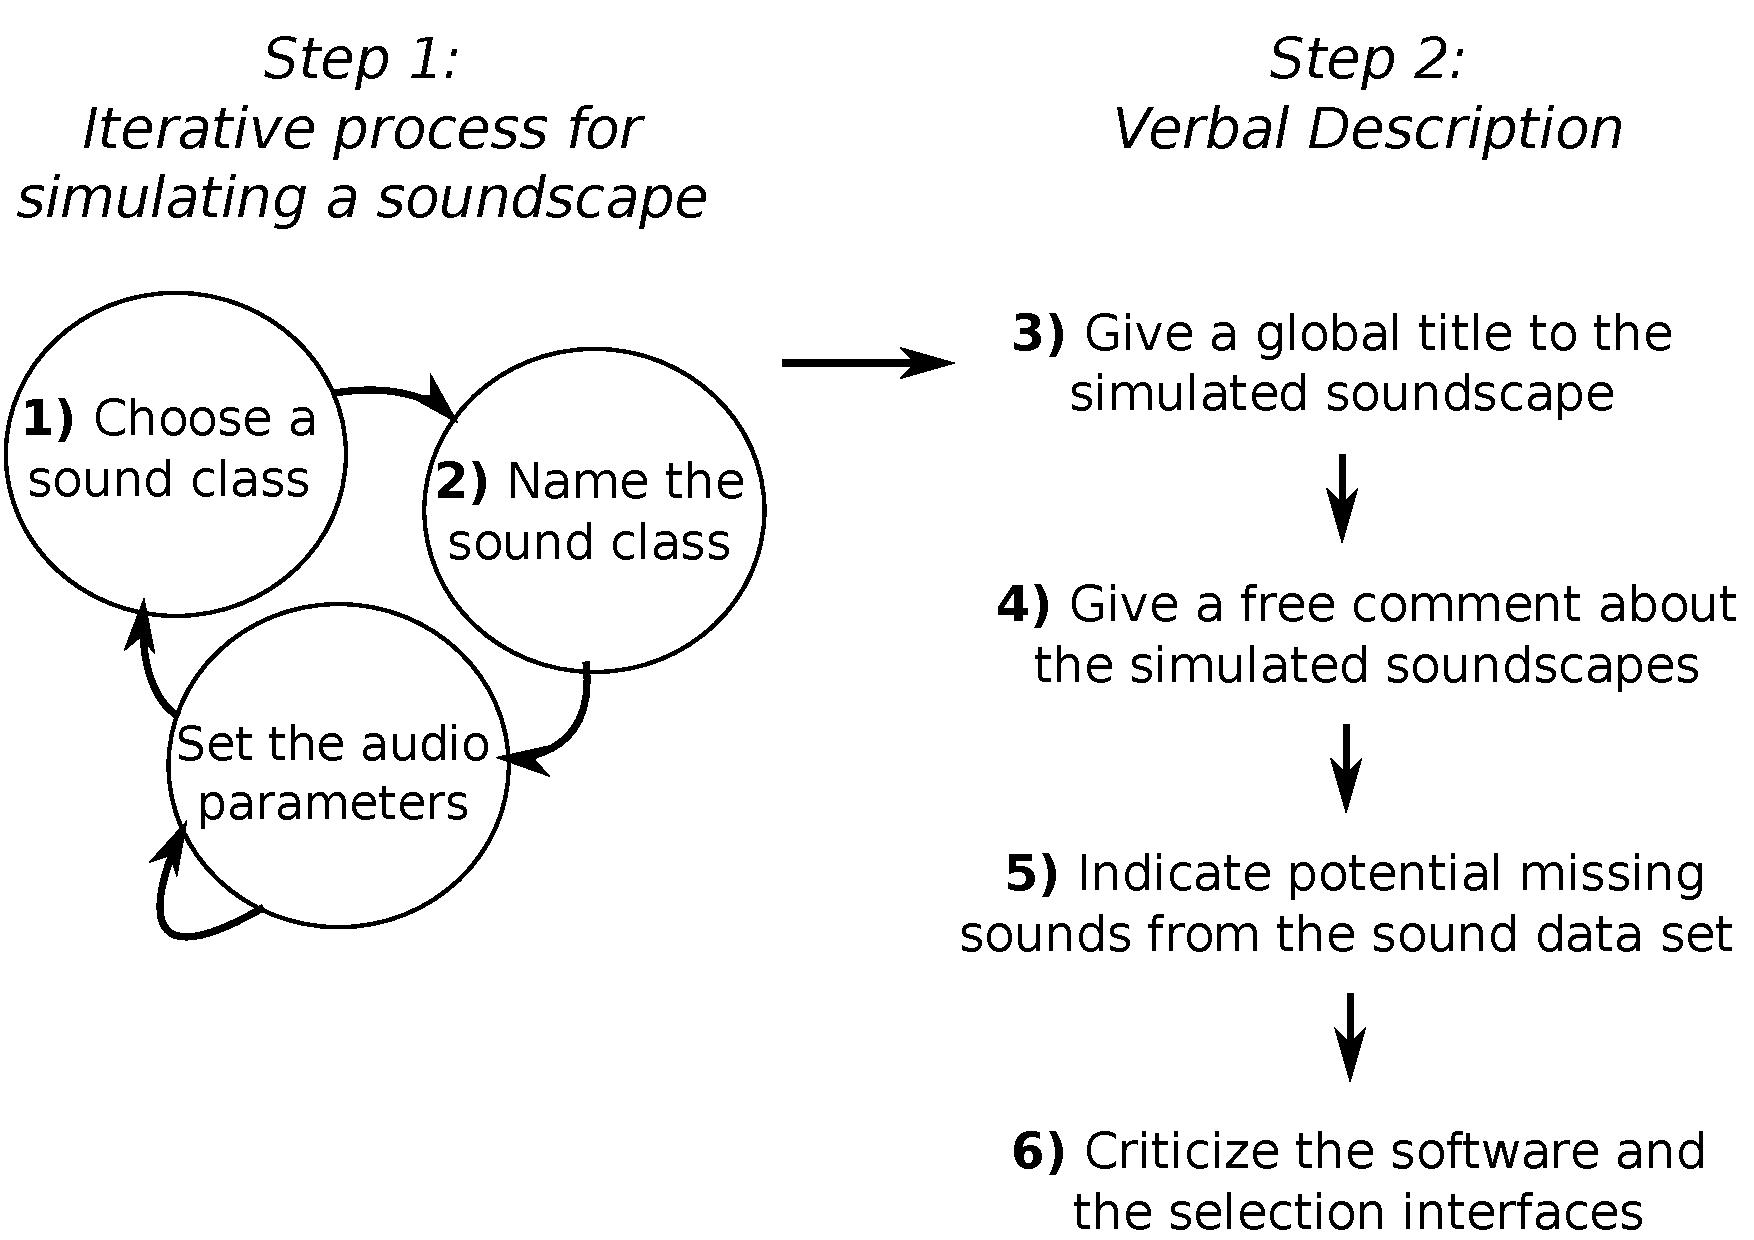
\includegraphics[width=.8\linewidth]{gfx/ch_4/4}
       \caption{Etape de processus de simulation pour l'analyse sensorielle}\label{fig:etapeSimu}
\end{figure}

Trois étapes composent le processus de simulation (\cf~Figure~\ref{fig:etapeSimu}):

\begin{itemize}
\item \emph{sélection} d'une classe de sons. Une fois une classe sélectionnée, une piste est générée; 
\item \emph{identification} de la classe de sons sélectionnée. Le sujet nomme la classe de sons qu'il a sélectionnée;
\item \emph{paramétrisation} de la piste liée à la classe de sons. Le sujet fixe les paramètres de la piste (pour plus de détails sur les paramètres proposés \cf~Section~\ref{sec:ch4_param}).
\end{itemize}

Ces étapes peuvent être répétées, et dans n'importe quel ordre, le sujet pouvant agir rétroactivement sur les pistes déjà crées. A la fin de la simulation, et afin d'accumuler le maximum de connaissances sur la scène simulée, le sujet peut: 

\begin{itemize}
\item nommer l'environnement simulé;
\item fournir un commentaire libre décrivant son processus de création, ainsi que le paysage sonore qu'il a voulu illustrer.
\end{itemize}

\subsubsection{Paramètres de contrôle}
\label{sec:ch4_param}

Les paramètres du modèle permettent au sujet de contrôler la structure de chaque piste. Ils agissent sur tous les samples à la fois, et non sur un en particulier.

Parmi ces paramètres, on retrouve ceux introduits pour le modèle initial de scène sonore (\cf~Section~\ref{sec:ch4_modelParam} et~\ref{sec:ch4_modelForm}), à savoir:

\begin{itemize}
\item \emph{niveau sonore} ($dB$): pour chaque sample, les niveaux sont tirés aléatoirement à partir d'une distribution normale, paramétrée par le sujet en terme de moyenne et de variance;
\item \emph{espacement inter-onset} (seconde): (piste d'événements seulement) comme pour les niveaux, les espacements sont tirés aléatoirement à partir d'une distribution normale, paramétrée par le sujet en terme de moyenne et de variance;
\item \emph{début et fin} (seconde): le sujet fixe le début et la fin de chaque piste.
\end{itemize}

Afin de faciliter la simulation, deux paramètres supplémentaires sont proposés:

\begin{itemize}
\item \emph{fondu par événement} (seconde): (piste d'événements seulement) le sujet fixe une durée de fondu (entrée et sortie), appliquée à chaque sample d'une piste d'événements;
\item \emph{fondu global} (seconde): le sujet fixe les durées de fondus séparément, pour l'entrée et la sortie de la piste. Ces fondus s'appliquent ainsi à l'ensemble des samples de la piste.
\end{itemize}

Deux de ces paramètres ne s’appliquent que pour les pistes d'événements (\emph{fondu par événement} et \emph{espacement inter-onset}), les samples des textures étant séquencés sans espacement (\cf~Section~\ref{sec:ch4_modelParam})

\subsubsection{Données produites par le processus de simulation}

\begin{figure}[t]
        \myfloatalign
        \includegraphics[width=.8\linewidth]{gfx/ch_4/schemaXP}
       \caption{Paradigme du protocole expérimental basé sur la simulation.}\label{fig:paradigmeSimu2}
\end{figure}

Ce protocole de simulation peut potentiellement produire un grand nombre de données. Ces dernières sont décrites à la figure~\ref{fig:paradigmeSimu2}.  Nous les résumons dans la liste suivante:

\begin{itemize}
\item données sémantiques objectives: la banque de données nous permet d'obtenir une information objective quant aux sources sonores présentes dans la scène. Les données sémantiques objectives sont les labels des classes sélectionnées;
\item données sémantiques subjectives: il s'agit des noms donnés par le sujet 1) à la scène simulée, 2) aux classes de sons sélectionnées;
\item données quantitatives issues de la partition: il s'agit de toutes les données relatives à la partition, \ie~pour chaque piste, le positionnement des samples et les paramètres (\cf~Section~\ref{sec:ch4_modelParam});
\item données quantitatives issues du signal: il s'agit d'indicateurs acoustiques extraits du signal, \eg~le niveau sonore global. Comme nous possédons les samples isolés utilisés pour la synthèse, il est possible de calculer ces descripteurs pour une classe, ou un ensemble de classes, en particulier.
\end{itemize}

Le protocole nous permet de caractériser avec précision une scène simulée, sur la base de données sémantiques, subjectives ou objectives, ainsi que quantitatives. Considérant l'ensemble des données générées, les potentiels d'analyse sont vastes.

\subsubsection{Interface de sélection aveugle des sons isolés}
\label{sec:ch4_ssf}

\begin{figure}[t]
        \myfloatalign
        \includegraphics[width=.8\linewidth]{gfx/ch_4/SSF}
       \caption{L'interface de sélection aveugle de l'outil de simulation \emph{Simscene}.}\label{fig:ssf}
\end{figure}

Pour limiter l’influence de l’interface sur le sujet, il nous paraît nécessaire de libérer sa recherche de toute information textuelle. Nous proposons à l'utilisateur une interface graphique lui permettant d’explorer la banque de sons exclusivement à partir de l’écoute.

Visuellement, les classes du dernier niveau (les seules accessibles par le sujet) sont représentées par des cercles, et positionnées sur un plan. La disposition des cercles dans l'espace dépend de l’organisation hiérarchique de la base de données: les sous-classes appartenant à la même classe sont proches les unes des autres, et ainsi de suite jusqu'à atteindre les classes des niveaux d'abstraction élevés.

La figure~\ref{fig:ssf} présente l'interface pour la banque de données d'événements sonores. Cette organisation visuelle à été pensée afin de:

\begin{enumerate}
\item faciliter le parcours de la banque de données, les sons similaires (au sens des classes) étant proches les uns des autres. L'organisation hiérarchique se fonde, en effet, sur des principes cognitifs. Les classes ont été établies à partir de la littérature traitant des catégories de sources sonores (\cf~Section~\ref{sec:ch4_collecSons}).
\item permettre aux sujets de rapidement appréhender toute l'étendue de la banque de données, \ie~l'ensemble des sons disponibles.
\end{enumerate}

Chaque classe possède un son prototype. Ces sons ont été choisis par les expérimentateurs. Lorsqu’on « clique » sur un cercle, le prototype associé à la classe est joué. Le sujet parcourt la banque de sons en cliquant sur les cercles. Cette interface a fait l'objet d'une étude approfondie dont les résultats sont publiés dans \citep{lafay2016JAES}.

%\gl{TODO: résumer les résultats JAES}

\subsubsection{Interface de simulation: l'outil \emph{Simscene}}
\label{sec:ch4_simscene}

\begin{figure}[t]
        \myfloatalign
        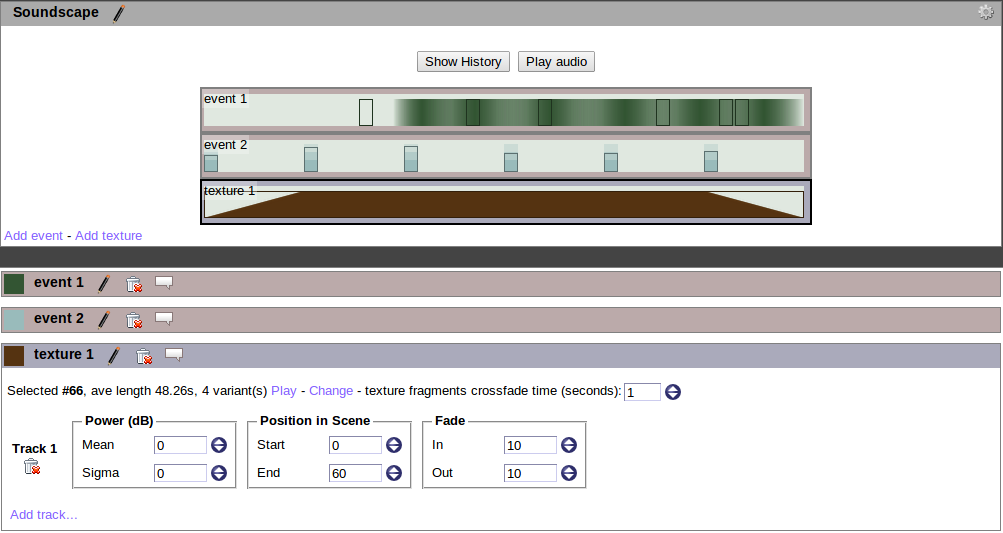
\includegraphics[width=\linewidth]{gfx/ch_4/simscene}
       \caption{L'outil de simulation \emph{Simscene}.}\label{fig:simscene}
\end{figure}

\emph{Simscene} est un environnement de travail audio-numérique, supporté par navigateur internet, et dont la première version a été développée dans le cadre du projet HOULE\footnote{Pour plus d’informations sur le Projet HOULE voir \url{http://houle.ircam.fr/}}. Il permet de simuler des paysages sonores à partir d'un corpus de sons. Il est prévu pour fonctionner sur les navigateurs internet \emph{Chrome} et \emph{Firefox}. L'outil a été développé en javascript à l'aide de la bibliothèque \emph{angular.js}\footnote{\emph{angular.js}: \cf~\url{https://angularjs.org/}} et du standard \emph{web-audio}\footnote{\emph{web-audio}: \cf~\url{http://www.w3.org/TR/webaudio/}}. L'interface de sélection (\cf~Section~\ref{sec:ch4_ssf}) a été développée à l'aide de la bibliothèque \emph{D3.js} \citep{d32011}.

\emph{Simscene} est présenté en détail dans \citep{rossignol2015simscene}. Nous résumons ici ses fonctionnalités d'importance pour notre étude. 

Le fonctionnement de \emph{Simscene} se rapproche de celui d'un séquenceur audio. Chaque utilisateur choisit une classe de sons via l'interface de sélection (\cf~Section~\ref{sec:ch4_ssf}). Une fois la classe de sons sélectionnée, une piste audio, liée à cette classe, est créée. L'utilisateur peut alors modifier certaines propriétés de la piste via un groupe de paramètres de contrôle propre à chacune (\cf~Section~\ref{sec:ch4_param}). Des champs de texte sont prévus afin de permettre à l'utilisateur 1) de nommer chaque piste, 2) de donner un titre à la scène simulée 3) de commenter la scène simulée.

L'interface propose un rendu graphique schématisé de la scène en cours de création (\cf~Figure~\ref{fig:simscene}). La piste est représentée par une bande possédant un axe temporel. Sur cette bande, chaque sample est représenté par un rectangle. L'espacement entre les rectangles est relatif à l'espacement entre les samples. De même, la hauteur des rectangles est proportionnelle au niveau sonore des samples. Dans le cas d'une piste de texture, un unique rectangle apparaît sur toute la longueur de la piste, un son de texture ne pouvant être entrecoupé de silences. Les caractéristiques des rectangles évoluent en fonction des changements de paramètres de la piste.

L'utilisateur a la possibilité, à tout moment, d'écouter la scène simulée.
 
%%%%%%%%%%%%%%%%%%%%%%%%%%%%%%%%%%%%%%%%%%%%%%%%%%%%%%%%%%%%%%%%%%%%%%%
%%%%%%%%%%%%%%%%%%%%%% XP 1      %%%%%%%%%%%%%%%%%%%%%%%%%%%%%%%%%%%%%%
%%%%%%%%%%%%%%%%%%%%%%%%%%%%%%%%%%%%%%%%%%%%%%%%%%%%%%%%%%%%%%%%%%%%%%%

\section[Agrément perçu et composition sémantique]{L'impact de la composition sémantique des scènes sur la perception de l'agrément}
\label{sec:xp1_2}

\subsection{Objectif}

L'objectif est d'étudier les influences spécifiques des différentes sources sonores qui composent les environnements urbains, sur la perception de l'agrément, en utilisant la simulation. Pour ce faire, nous planifions nos deux premières expériences (\cf~Figure~\ref{fig:xp1_2}):

\begin{itemize}
\item \emph{expérience de simulation}: au cours de cette expérience, les sujets doivent simuler des environnements sonores urbains, en utilisant l'outil et le protocole de simulation décrits à la section~\ref{sec:ch4_simscene}. Chacun compose deux environnements sonores urbains, le premier idéal/agréable et le deuxième non-idéal/désagréable. Cette épreuve de simulation a fait l'objet d'une expérience pilote \citep{lafay2013atiam,lafay2014new}; 

%\gl{TODO: préciser xp pilote}

\item \emph{expérience d'évaluation}: à l'issue de la simulation, nous n'avons, de fait, qu'une connaissance binaire des propriétés affectives des scènes simulées: idéale (i) et non-idéale (ni). Cette seconde étape a pour but d'affiner notre connaissance sur l'agrément. Pour ce faire, nous demandons à un deuxième groupe de sujets d'évaluer, à partir d'une échelle sémantique, l'agrément de chacune des scènes simulées. L'expérience d'évaluation sert deux buts:

\begin{enumerate}
\item évaluer l'influence respective des différentes sources sur l'agrément, pour chaque type d'environnement (i ou ni);
\item détecter la présence de cas extrêmes ou ambigus (\emph{outlier}) dans les scènes simulées. Pour le reste de notre étude, les qualités hédoniques imposées (i et ni) servent de référence, de vérité terrain. Il nous faut donc garantir qu'il n'y ait pas d’ambiguïté entre les cas extrêmes des i- et ni-scènes, \ie~que la note d'agrément la plus basse des i-scènes reste supérieure à la note la plus haute des ni-scènes.
\end{enumerate}

\end{itemize}

Notre analyse s'appuie sur les données produites par les deux expériences.

\begin{figure}[t]
        \myfloatalign
        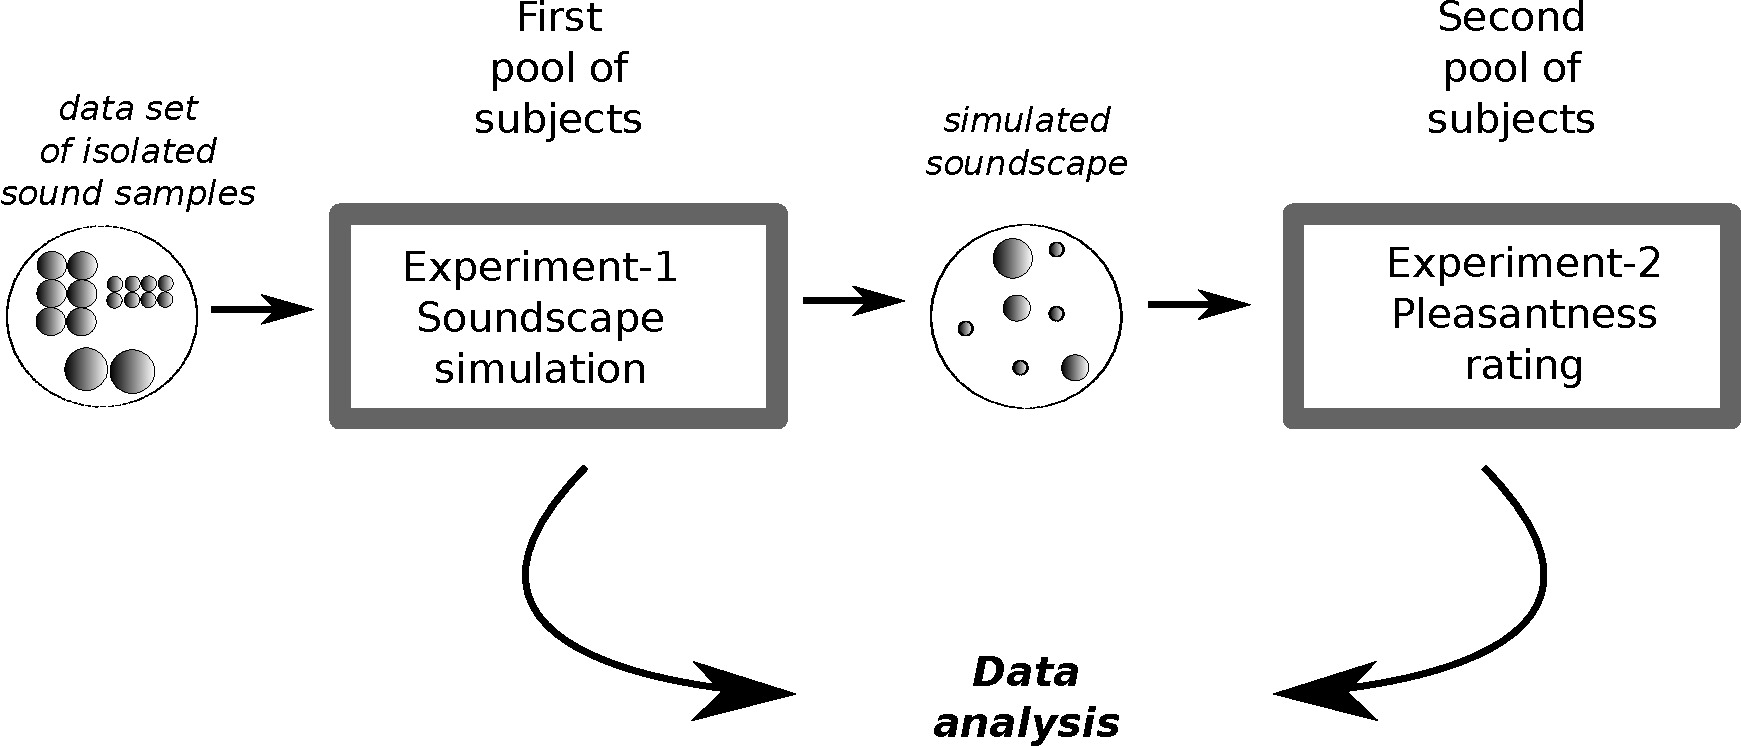
\includegraphics[width=.8\linewidth]{gfx/ch_5/5}
        \caption{Planification expérimentale des éxperiences de simulation et d'évaluation de l'agrément}\label{fig:xp1_2}
\end{figure}

\subsection{Banque de données de sons isolés}

Dans cette partie, nous présentons les processus de sélection et d'acquisition des sons utilisés comme matériau de base lors de la simulation des environnements sonores urbains. La banque de données est identique à celle utilisée dans le cadre de l'expérience pilote \citep{lafay2013atiam,lafay2014new}. 

Pour plus de détails sur l'organisation interne de la banque de données, ainsi que sur l'interface graphique permettant de sélectionner ces dernières, se référer aux sections~\ref{sec:ch4_dbEventTexture} et~\ref{sec:ch4_ssf}.

\subsection[Typologie des sources sonores]{Typologie des sources sonores présentes dans l'environnement urbain}

Afin de créer un corpus de sons isolés de référence pour la simulation, nous réalisons une typologie des sons environnementaux urbains. 

Pour ce faire, une étude bibliographique est effectuée, afin d'identifier les sources et ambiances sonores les plus souvent citées dans les publications. Cette étude porte sur 16 articles ou thèses. Chacun d'eux traite de la manière dont nous discriminons les paysages sonores urbains. Il ressort que plusieurs approches sont possibles:

\begin{itemize}
\item 9 articles abordent le problème par une approche perceptive, soit en identifiant ou répertoriant des catégories de sources sonores, soit en étudiant l'impact de classes de sons spécifiques sur la perception de l'environnement: \cite{maffiolo_caracterisation_1999,raimbault2002simulation,guastavino_etude_2003,defreville2004aactivity,raimbault2005urban,dubois2006cognitive,devergie_relations_2006,guastavino2006ideal,niessen2010categories}
\item 3 articles proposent une classification morpho-typologique, divisant l’environnement sonore urbain en « zones sonores » possédant une identité acoustique forte, selon la configuration et la pratique du site: \cite{maffiolo_caracterisation_1999,beaumont2004pertinence,polack2008perceptive}
\item 2 articles répertorient et classifient les sources sonores d’un point de vue expert: \cite{leobon_analyse_1986,brown2011towards}
\end{itemize}

La nature des classes est établie par rapport aux catégories perceptives, ou classes de sons, émergeant de cette littérature. À partir des éléments relevés, nous établissons deux taxonomies, une pour les événements (\cf~Figures~\ref{fig:taxonomieEventa} et~\ref{fig:taxonomieEventb}), une autre pour les textures (\cf~Figures~\ref{fig:taxonomieTexturea} et~\ref{fig:taxonomieTextureb}). Comme évoqué à la section~\ref{sec:ch4_sourceAction}, la structure taxonomique de ces deux ensembles s'inspire grandement de l'axe vertical de l'organisation catégorielle proposée par E. Rosch (\cf~Section~\ref{sec:ch3_categoEtAbstract}), \ie~plus le niveau d'abstraction de la classe est élevé, plus la description de la classe est précise, et plus les sources sonores incluses dans cette classe sont semblables (\cf~Figure~\ref{fig:orgDb}). Pour les événements, nous considérons quatre niveaux d'abstraction allant des classes les plus globalisantes (niveau d'abstraction 0), aux classes les plus spécifiques (niveau d'abstraction 3). Pour les textures, nous ne considérons que trois niveaux d'abstraction.

Pour les événements, les regroupements se font essentiellement par rapport à la source, et sont d’ordre sémantique. Pour les textures, nous considérons également la nature des lieux hébergeant ces sources (\eg~\emph{parc}, \emph{rue}). La typologie des classes d'événements suit la nomenclature source-action introduite à la section (\cf~Section~\ref{sec:ch4_sourceAction}). Elle est assez proche d'une autre typologie des sources sonores urbaines introduite ultérieurement \citep{Salamon14}.

Les réactions à la musique étant trop subjectives, et les jugements esthétiques ne pouvant qu'altérer les données d'évaluation, nous choisissons, dans cette étude, de ne pas considérer les sources musicales de type musiciens de rue, radios de voitures, d'appartements, \etc. 
 
\begin{figure}[t]
        \myfloatalign
        \subfloat[]
        {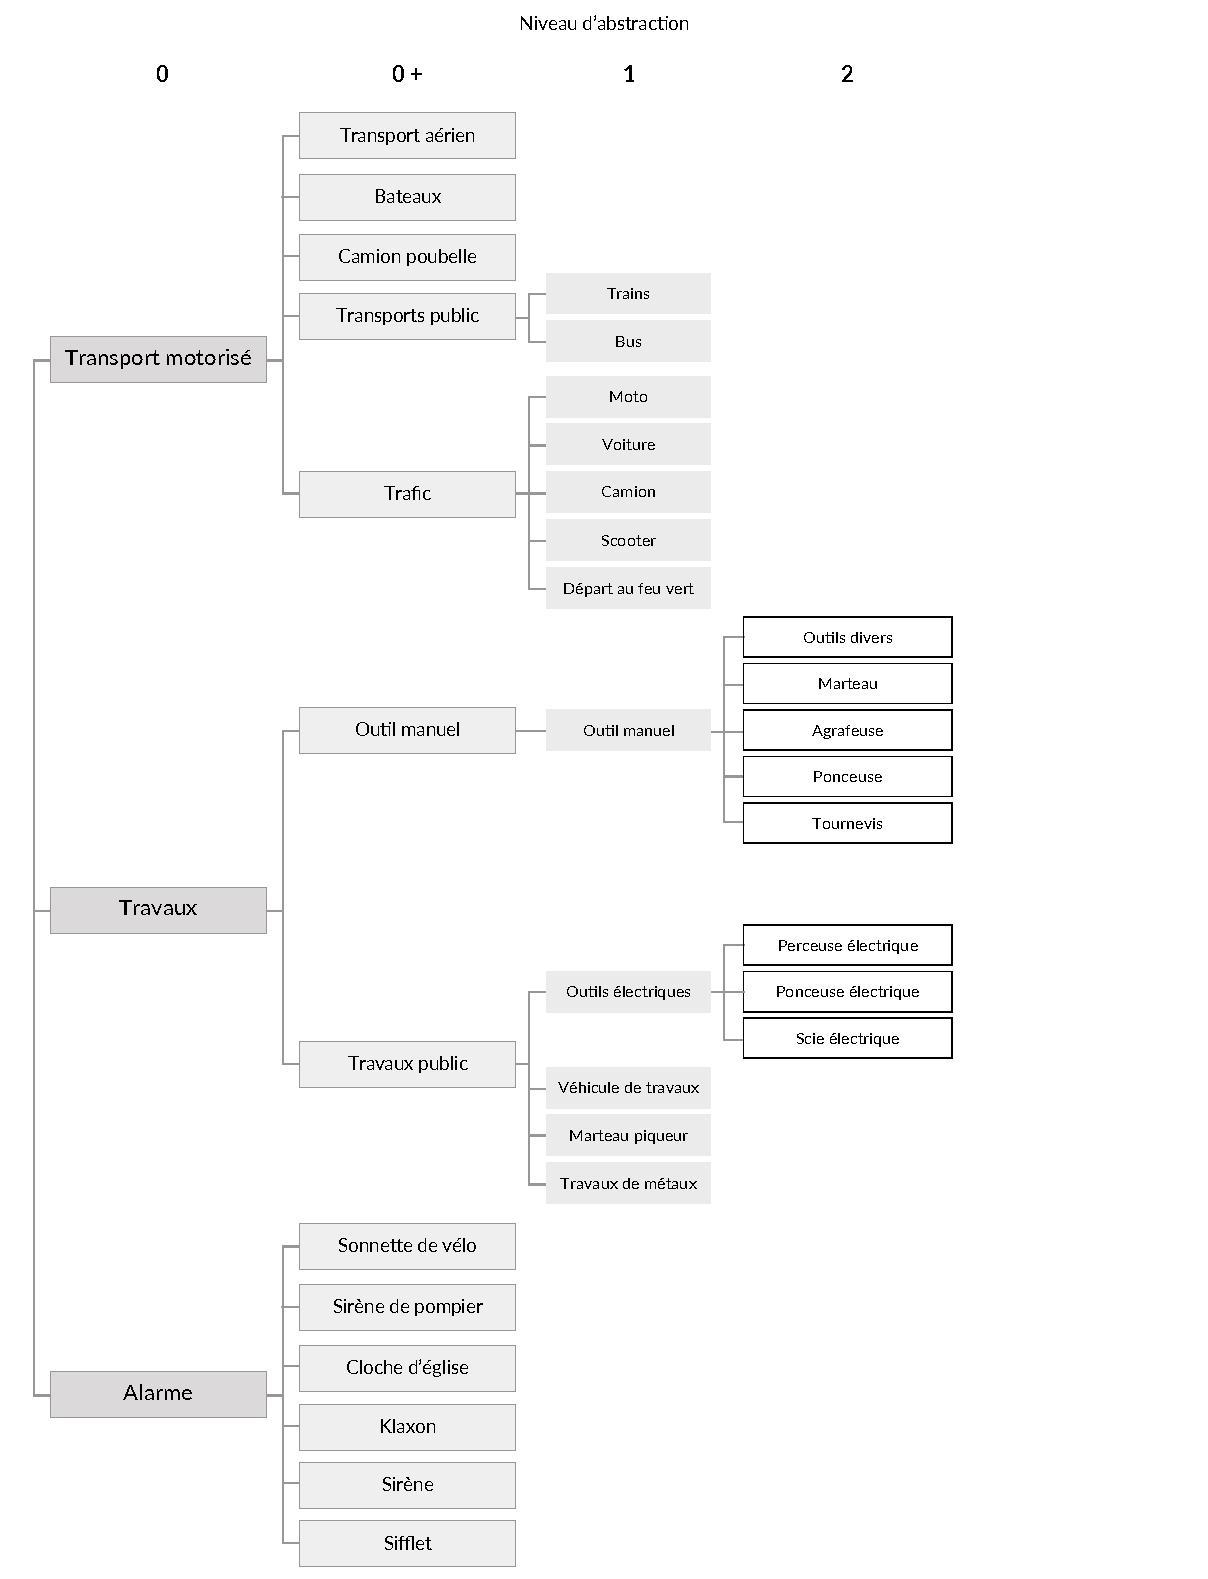
\includegraphics[width=.45\columnwidth]{gfx/ch_5/event_1}\label{fig:taxonomieEventa}}
        \subfloat[]
        {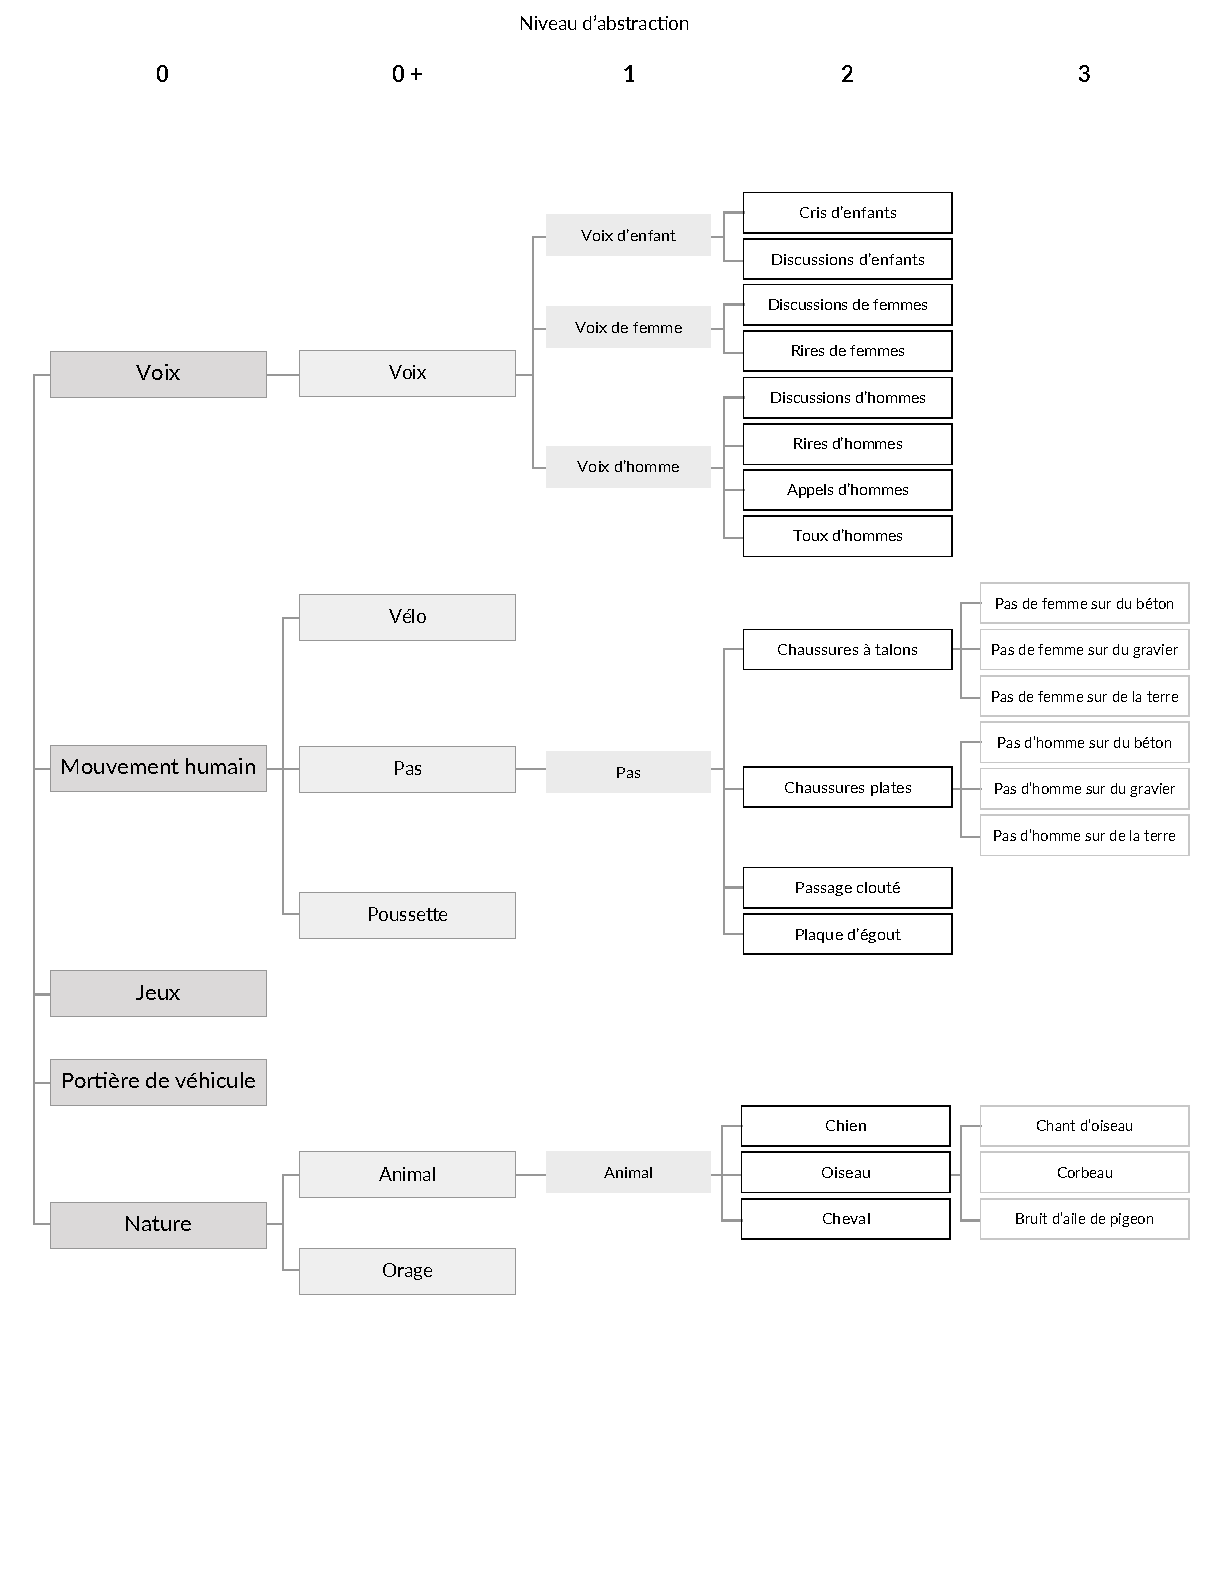
\includegraphics[width=.45\columnwidth]{gfx/ch_5/event_2}\label{fig:taxonomieEventb}}\par
        \subfloat[]
        {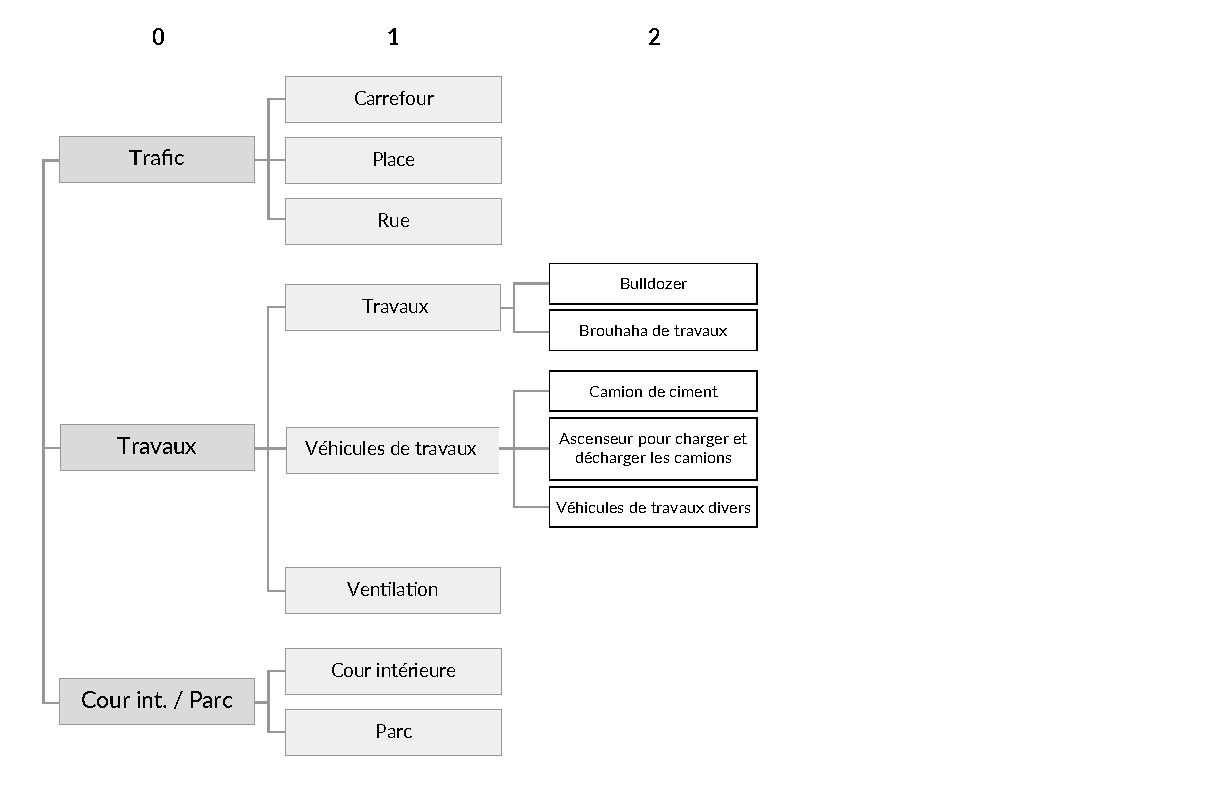
\includegraphics[width=.45\columnwidth]{gfx/ch_5/texture_1}\label{fig:taxonomieTexturea}}
        \subfloat[]
        {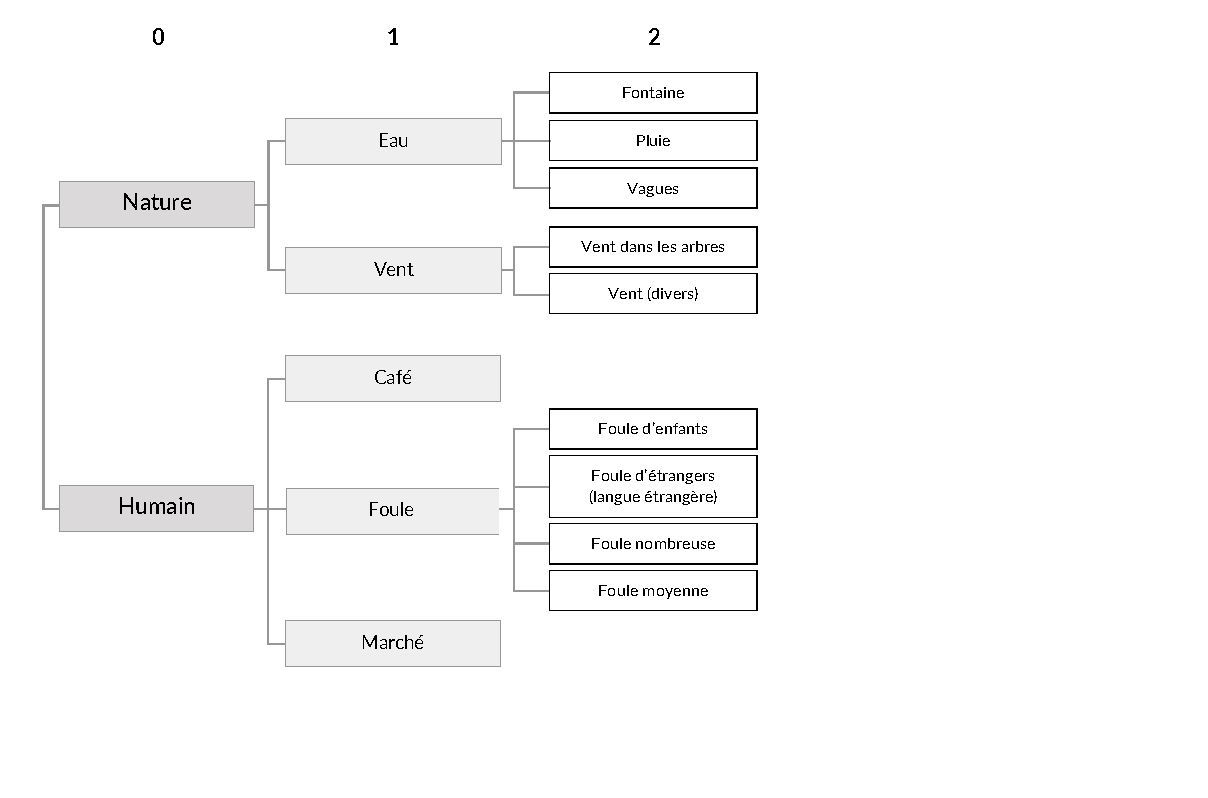
\includegraphics[width=.45\columnwidth]{gfx/ch_5/texture_2}\label{fig:taxonomieTextureb}}
       \caption[Taxonomies des classes de sons utilisées pour la simulation des environnements sonores urbains.]{Taxonomies des classes de sons utilisées pour la simulation des environnements sonores urbains pour (a,b) les événements sonores et (c,d) les textures sonores.}\label{fig:taxonomie}
\end{figure}

\subsection{Acquisition des sons isolés}
\label{sec:ch5_recordDataSet}

Sur la base des typologies précédemment établies, 483 sons ont été collectés, dont 381 événements, et 102 textures.

Parmi les événements:

\begin{itemize}
\item 260 sont issus d’enregistrements effectués pour l'étude;
\item 89 sont issus de la banque de sons \emph{SoundIdeas}\footnote{Pour plus de détails sur \emph{SoundIdeas} voir :\url{ http://www.sound-ideas.com/}};
\item 32 sont issus de la banque de sons \emph{Universal SoundBank}\footnote{Pour plus de détails sur \emph{Universal SoundBank} voir : \url{http://www.universal-soundbank.com/}}.
\end{itemize}

Parmi les textures:

\begin{itemize}
\item 72 sont issues d’enregistrements effectués pour l'étude;
\item 23 sont issues de la banque de sons \emph{SoundIdeas};
\item 7 sont issues de la banque de sons \emph{Universal SoundBank}.
\end{itemize}

Tous les enregistrements ont été effectués à l’aide d'un micro canon \emph{AT8035}\footnote{\cf~\url{http://eu.audio-technica.com/fr/products/product.asp?catID=1&subID=6&prodID=1845}} relié à un enregistreur \emph{ZOOM H4n}\footnote{\cf~\url{http://www.zoom.co.jp/english/products/h4n/}}. L’utilisation du micro canon nous permet d’isoler les événements sonores du brouhaha urbain. Pour les textures, il nous permet d’éviter les événements sonores proches du preneur de son. Nous pouvons ainsi pointer des "zones sonores", en nous tenant à une certaine distance de ces dernières, afin de capter uniquement le brouhaha émanant de la zone ciblée.

Tous les sons ont été normalisés au même niveau $RMS$ \footnote{Le niveau $RMS$, de l'anglais \emph{Root Mean Square} qui désigne la valeur efficace d'un signal. Formellement, le niveau $RMS$ $x_{RMS}$ d'un signal $x=(x_1,x_2,\ldots,x_n)$ s'obtient en calculant la moyenne quadratique de ce dernier $x_{RMS}=\sqrt{\dfrac{1}{n}\sum\limits_{i} x_i^2}$.} de $-12$ $dB$ (FS) \footnote{$dB$ (FS) est le sigle anglais désignant une valeur en décibels relative à la pleine échelle (\emph{relative to Full Scale}), \ie~le rapport entre le niveau du signal et sa valeur maximale. Dans notre cas, ce niveau pleine échelle est de 1 Volt.}.

\subsection{Planification expérimentale}

\subsubsection{Épreuve de simulation}
\label{sec:ch5_planExpSimu}

Nous nommons cette expérience: \emph{expérience 1.a}. \\

{\setlength{\parindent}{0cm}\textbf{Procédure}} \\

Les sujets doivent simuler deux environnements sonores urbains, chacune des scènes devant durer 1 minute. Pour ces simulations, les sujets doivent se conformer aux consignes suivantes:

\begin{itemize}
\item première simulation: simuler un paysage sonore \textbf{urbain plausible} qui, selon vous, est idéal (où vous aimeriez vivre);
\item deuxième simulation: simuler un paysage sonore \textbf{urbain plausible} qui, selon vous, est non-idéal (où vous n'aimeriez pas vivre).
\end{itemize}

Tous les sujets commencent par simuler l'environnement idéal. Les sujets ne prennent connaissance de la deuxième consigne qu'à la fin de la première simulation.

Les sujets sont totalement libres dans le choix des sons, et des paramètres (pour plus de détails sur les paramètres se référer à la section~\ref{sec:ch4_param}). Ils doivent cependant se soumettre à deux contraintes:

\begin{itemize}
\item le sujet doit prendre le point de vue d’un auditeur fixe;

\item le paysage sonore doit être réaliste, au sens de physiquement plausible. Autrement dit, le sujet à tout à fait le droit de placer 10 chiens dans son paysage sonore, mais il n’a pas le droit de placer un chien aboyant toutes les 10 millisecondes.

\end{itemize}

Ces contraintes font partie de la consigne. Aucun contrôle n'est fait \emph{a priori} dans l'interface de simulation.

Chaque processus de simulation comprend deux parties:

\begin{enumerate}
\item la réalisation de la simulation: cette étape peut, elle même, se décomposer en trois actions (\cf~Section~\ref{sec:ch4_processSimu}):
\begin{itemize}
\item sélectionner les classes de sons
\item nommer les classes de sons sélectionnées
\item paramétrer les pistes (\cf~Section~\ref{sec:ch4_seqSample}) relatives aux classes de sons sélectionnées
\end{itemize}
\item la production d'un commentaire libre du paysage sonore simulé
\end{enumerate}

En complément, et une fois les deux scènes sonores réalisées, les sujets sont invités à:

\begin{itemize}
\item indiquer les sources sonores qu'ils voulaient mettre, mais qu'ils n'ont pas trouvées;
\item commenter l’ergonomie du logiciel de simulation;
\item commenter l’ergonomie de l'interface de sélection.
\end{itemize}

Avant de commencer la première simulation, un tutoriel de 20 minutes est proposé aux sujets, afin qu'ils se familiarisent avec le logiciel de simulation, et la banque de données. Le tableau~\ref{tab:indSimu} résume les étapes de l’expérience, ainsi que leurs durées respectives. L'expérience est prévue pour durer 2h30. \\

\begin{table}[t]
\centering
\begin{tabular}{c c c} 
Index          & Tâche                               & Durée (min) \\                      
\hline
1 & Présentation de l'expérience                     & 10 \\
  & Lecture de la consigne                           &  \\
\hline
2 & Tutoriel (Réalisation d'une scène test)          & 20 \\
\hline
3 & Première simulation: scène idéale                & 40 \\
\hline
4  & Commentaire de la scène idéale                  & 15 \\
\hline
3 & Deuxième simulation: scène non-idéale            & 40  \\
\hline
4  & Commentaire de la scène non-idéale              & 15 \\
\hline
5 & Critique de l'interface de simulation            & 10 \\
  & et de l'interface de sélection                   & \\
\hline
\end{tabular}
\vspace{0.5mm}
\caption{Résumé des étapes de l’expérience de simulation.}
\label{tab:indSimu}
\end{table}

{\setlength{\parindent}{0cm}\textbf{Dispositif expérimental}} \\

Tous les sujets passent l'expérience sur des machines identiques. L'audio est diffusé en stéréophonie, par le biais de casques audio. Pendant le tutoriel, les sujets doivent ajuster le niveau sonore à un volume confortable. Ils ne peuvent le modifier par la suite.

Tous les sujets réalisent l'expérience simultanément. Ils sont répartis de manière égale dans trois pièces identiques, toutes possédant un environnement calme. Ils n'ont pas le droit de s'adresser la parole pendant l'expérience.

Trois expérimentateurs, un dans chaque pièce, sont présents durant la totalité de l'expérience, afin de contrôler le bon déroulement de cette dernière, et de répondre aux éventuelles questions des sujets.  \\

{\setlength{\parindent}{0cm}\textbf{Participants}} \\

44 étudiants (14 femmes) de L’École Centrale de Nantes ont participé à l'expérience. Ils ont tous sensiblement le même âge (moyenne: 21.6, écart-type: 2). Tous les sujets sont Nantais, et vivent dans cette ville depuis deux ans ou plus.

Sur les 44 sujets, 40 réalisent l'expérience avec succès, produisant au final 80 scènes sonores simulées, dont 40 scènes idéales, et 40 scènes non idéales. 4 sont éliminés pour non respect ou incompréhension des consignes, d'une part, et dépassement du temps, d'autre part.

\subsubsection{Épreuve d'évaluation de l'agrément}
\label{sec:ch5_planExpEvaA}

Nous nommons cette expérience: \emph{expérience 1.b}. \\

{\setlength{\parindent}{0cm}\textbf{Procédure}} \\

En raison de contraintes temporelles, les sujets n'évaluent que des séquences de 30 secondes des scènes simulées, chacune de ces séquences commençant à la seconde 15, et finissant à le seconde 45 de la scène d'une durée d'origine de 1 minute.

L'évaluation s'effectue sur une échelle sémantique bipolaire de 7 points, allant de -3 (non-idéale/très désagréable) à +3 (idéale/très agréable). Avant de noter une scène, les sujets doivent obligatoirement écouter les 20 premières secondes de cette dernière. Après la notation, ils sont libres de passer à la scène suivante.

Pour chaque sujet, les scènes sont présentées dans un ordre aléatoire. Les 10 premières scènes permettent au sujet de calibrer ses notes. Elles sont obligatoirement composées de 5 scènes idéales, et de 5 scènes non-idéales. Ces 10 premières scènes sont rejouées à la fin de l'expérience, et seules les notes données à la deuxième occurrence sont prises en compte. 

L'expérience est prévue pour durer 30 minutes. Les sujets ne connaissent pas la nature des scènes.\\

{\setlength{\parindent}{0cm}\textbf{Dispositif expérimental}} \\

Tous les sujets passent l'expérience sur des machines identiques. L'audio est diffusé en stéréophonie, par le biais de casques audio semi-ouverts \emph{Beyer-Dynamic DT 990 Pro}. Toutes les scènes sonores ont été re-simulées sur la base des partitions obtenues lors de l'expérience de simulation. Le niveau sonore de sortie est identique pour tous les sujets.

Tous les sujets réalisent l'expérience simultanément, dans un environnement calme. Ils n'ont pas le droit de s'adresser la parole pendant l'expérience. 

Un expérimentateur est présent durant la totalité de l'expérience, afin de contrôler le bon déroulement de celle-ci, et de répondre aux éventuelles questions des sujets.  \\

{\setlength{\parindent}{0cm}\textbf{Participants}} \\

10 étudiants (2 femmes) de L’École Centrale de Nantes ont participé à l'expérience. Aucun d'entre eux n'a réalisé l'expérience de simulation. Tous les sujets ont sensiblement le même âge (moyenne: 23.1, écart-type: 1.8). Tous les sujets sont Nantais, et vivent dans cette ville depuis deux ans ou plus.

Tous les sujets ont réalisé l'expérience avec succès.

\subsection{Données et méthodes d'analyses}

\subsubsection{Nature des données analysées}
\label{sec:ch5_dataType1}

A partir des données produites par l'épreuve de simulation, nous analysons:

\begin{itemize}
\item les partitions des scènes simulées;
\item les signaux des scènes simulées;
\item les commentaires sur les sons manquants, et l'ergonomie des interfaces de simulation et de sélection.
\end{itemize}

Chaque scène est décrite par un groupe de descripteurs. C'est sur ces descripteurs que nous pratiquons l'analyse. Un résumé des descripteurs, ainsi que des acronymes les désignant, est présenté dans le Tableau~\ref{tab:acronyme}. Afin de rester cohérent avec l'épreuve d'évaluation, les descripteurs issus des partitions, ou des signaux des scènes, ne sont pas calculés sur la durée totale de celles-ci, mais sur une version réduite de 30 secondes (\cf~Section~\ref{sec:ch5_planExpEvaA}). 

Pour chaque scène sonore, trois types de descripteurs sont considérés:

\begin{itemize}
\item \emph{perceptif}: il s'agit de l'agrément perçu de la scène simulée, évalué sur une échelle sémantique de 7 points. Nous notons $\mathcal{A}_{scene}$ l'agrément moyen d'une scène, obtenu en moyennant les notes de tous les sujets. De même, nous notons  $\mathcal{A}_{sujet}$ l'agrément par sujet, en moyennant l'ensemble de ses notes. Compte tenu du faible nombre de sujets, nous faisons le choix, dans cette étude, de ne pas normaliser les notes d'agrément;
\item \emph{sémantique}: il s'agit d'un vecteur booléen noté $S=(x_1,x_2,\ldots,x_n)$, indiquant les classes de sons présentes dans la scène. Chaque point $x$ de ce vecteur correspond à une classe de sons particulière: $x=1$ si la classe est présente dans la scène, et $x=0$ autrement. La dimension $n$ des vecteurs dépend du niveau d'abstraction considéré, \eg~pour le niveau d'abstraction 1, qui comprend $44$ classes de sons, cette dimension sera de $n=44$.
\item \emph{structurel}: les descripteurs structurels sont calculés à partir des partitions et des signaux des scènes simulées. Trois descripteurs structurels sont envisagés:
\begin{itemize}
\item \emph{diversité} ($DIV$): il s'agit d'un scalaire représentant la diversité des classes sonores utilisées pour simuler une scène. Nous calculons $DIV$ en comptant le nombre de classes de sons distinctes utilisées pour une simulation. Ce nombre dépend du niveau d'abstraction considéré. Par exemple, considérant les deux sous classes du niveau d'abstraction 2 \emph{passage de voiture} et \emph{démarrage de voiture}, toutes deux appartenant à la classe \emph{voiture} du niveau d'abstraction 1, nous comptons deux classes pour la diversité des niveaux d'abstraction 2, et 1, et seulement 1, pour les niveaux d'abstraction 0 et 1;
\item \emph{densité} ($D$): il s'agit d'un scalaire représentant le nombre de sources sonores présentes en moyenne. Pour obtenir $D$, nous calculons le logarithme du nombre d'éléments sonores par fenêtre de 125 millisecondes (sans recouvrement), et moyennons au cours du temps. Le calcul de $D$ peut inclure toutes les sources sonores de la scène, ou seulement une partie. Dans ce cas, les fenêtres ne contenant pas de sources sonores ne sont pas prises en compte. Nous notons $D(E)$ et $D(T)$ les densités calculées en considérant séparément les sources d'événements et de textures sonores;
\item \emph{niveau Sonore} ($L$): pour représenter le niveau sonore, nous nous inspirons de la mesure $L_{Aeq}$. Dans notre cas, il s'agit d'un scalaire, calculé sur le signal en volts, et non en pression, et donné en décibels, en prenant un référentiel de 1 Volt. Le niveau est obtenu en calculant, toutes les secondes, la moyenne quadratique du signal, et en moyennant sur la durée de la scène. Un filtrage de type A est opéré avant le calcul des moyennes quadratiques. D'autre descripteurs, inspirés eux aussi de descripteurs acoustiques classiques ($L_{Amin}$, $L_{Amax}$, $L_{A10-90}$), et utilisant un opérateur autre que la moyenne (minimum, maximum, les 10-90ème quantiles) pour intégrer les fenêtres de 1 seconde, ont été testés. Mais, ces derniers présentant tous une corrélation élevée avec $L$ ($r_{pearson}\geq0.76$, $p<0.01$), nous conservons le scalaire ci-devant mentionné comme unique descripteur objectif du niveau sonore.
\end{itemize}
\end{itemize}

\begin{table}[t]
\centering
\begin{tabular}{c c c c c} 
Descripteurs          & Acronymes   &   & Descripteurs            & Acronymes  \\                       
\cline{1-2} \cline{4-5}
Densité               & $D$         &   & Diversité               & $DIV$    \\
                      &             &   &                         &          \\
Densité               & $D(E)$      &   & Diversité               & $DIV(E)$ \\
(événements)          &             &   & (événements)            &          \\
Niveau                & $L$         &   & Diversité               & $DIV(T)$ \\
                      &             &   & (textures)              &          \\
Niveau                & $L(E)$      &   & Agrément moyen          & $\mathcal{A}_{scene}$     \\
(événements)          &             &   & (par scène)             &         \\
Niveau                & $L(T)$      &   & Agrément moyen          & $\mathcal{A}_{sujet}$        \\
(textures)            &             &   & (par sujet)             &      \\
                      &             &   &                         &      \\
\multicolumn{3}{c}{Termes} &  \multicolumn{2}{c}{Acronymes} \\ 
\hline
\multicolumn{3}{c}{Idéal/agréable}                 & \multicolumn{2}{c}{i}       \\
\multicolumn{3}{c}{non-idéale/désagréable}         & \multicolumn{2}{c}{ni}      \\
\multicolumn{3}{c}{Scène idéale/agréable}          & \multicolumn{2}{c}{i-scène} \\
\multicolumn{3}{c}{Scène non-idéale/désagréable}   & \multicolumn{2}{c}{ni-scène} \\
\hline
\end{tabular}
\vspace{0.5mm}
\caption{Acronyme des variables utilisées dans le cadre des expériences sensorielles.}
\label{tab:acronyme}
\end{table}


\subsubsection{Méthodologie et Outils statistiques}
\label{sec:ch5_methodoEtStat1}

Afin d'évaluer l'impact spécifique des différentes sources sonores sur l'agrément perçu, nous soumettons nos travaux aux 6 tests/études de significativité présentés ci-après:

\begin{itemize}
\item \emph{étude qualitative}: afin de vérifier la validité écologique de 1) la banque de données et 2) l'interface de sélection, nous réalisons une étude qualitative des critiques ergonomiques effectuées par les sujets;
\item \emph{Vérification de l'agrément des scènes simulées}: afin de vérifier que la distinction affective imposée entre les i- et ni-scènes se retrouve au niveau de l'agrément perçu, nous observons s'il existe des différences entre les deux types de scène au niveau de $\mathcal{A}_{scene}$ et $\mathcal{A}_{sujet}$. La significativité est évaluée par un test de Student à deux populations indépendantes pour $\mathcal{A}_{scene}$, et par un test de Student à deux populations appariées pour $\mathcal{A}_{sujet}$ (\cf~Annexe~\ref{app:student});
\item \emph{étude comparative entre les descripteurs structurels}: afin d'évaluer si la distinction affective imposée entre les i- et ni-scènes impacte de manière significative la nature des scènes, \ie~s'il existe des différences significatives entre les descripteurs structurels et/ou l'agrément perçu, nous évaluons cette significativité à partir d'un test de Student à deux populations (\cf~Annexe~\ref{app:student});
\item \emph{étude de l'influence des descripteurs structurels sur l'agrément perçu}: afin d'évaluer l'impact potentiel des descripteurs structurels sur l'agrément perçu, nous étudions l'existence de corrélations linéaires entre ces deux types de descripteurs. Pour mesurer la corrélation, nous utilisons le coefficient de Pearson (\cf~Annexe~\ref{app:corr}). Nous adoptons ici une méthodologie couramment utilisée dans l'approche dimensionnelle;
\item \emph{étude comparative entre les descripteurs sémantiques}: afin d'apprécier si la distinction affective imposée a eu un impact sur la composition des scènes en termes de sources sonores, ou, pour être plus précis, s'il existe des classes de sons qui ont été particulièrement utilisées pour simuler un type d'environnement, nous utilisons le V-test. Nous vérifions si la présence d'une classe de sons est typique d'un environnement (i ou ni). Le test est effectué pour chaque niveau d'abstraction, et séparément, pour les classes d'événements et de textures. Pour chaque classe $j$ et chaque type d'environnements $k$ ($k={i,ni}$), la valeur $V_{jk}$ du V-test se calcule comme suit: 

\begin{equation*}
V_{jk}=\dfrac{c_{jk}-c_k\frac{c_j}{c}}{\sqrt{c_k\frac{c-c_k}{c-1}\frac{c_j}{c}(1-\frac{c_j}{c})}}
\end{equation*}

où $c$ est le nombre de classes utilisées, $c_k$ le nombre de classes utilisées pour un type d'environnement $k$, $c_j$ le nombre de classes $j$ utilisées, et $c_{jk}$ le nombre de classes $j$ utilisées pour un type d'environnement $k$. Le V-test teste l'hypothèse nulle que la proportion $\frac{c_{jk}}{c}$ ne diffère pas significativement de la proportion $\frac{c_{jk}}{c_k}$. Si pour un environnement $k$, et une classe $j$, l'hypothèse est rejetée, la classe $j$ est alors typique de l'environnement $k$. Les classes typiques sont nommées \textbf{marqueurs sonores};

\item \emph{étude des espaces de représentations induits par les descripteurs sémantiques}: afin d'étudier si une représentation basée uniquement sur la présence ou l'absence des classes de sons permet de séparer les deux types d'environnement, nous considérons l'espace induit par les descripteurs sémantiques $S$. $S$ étant un vecteur booléen, nous calculons les distances entre les scènes à partir de la distance de Hamming. Considérant les deux vecteurs $S_1=(x_{1,1},x_{1,2},\ldots,x_{1,n})$, et $S_2=(x_{2,1},x_{2,2},\ldots,x_{2,n})$ de dimension $n$, avec $x={0,1}$, la distance de Hamming $d_{ham}$ mesure le pourcentage de coordonnées qui diffèrent entre les deux vecteurs:   


\begin{equation*}
d_{ham}(S_1,S_2)=\dfrac{1}{n}\sum_{i=1}^{n} (x_{1,i} \bigoplus x_{2,i})
\end{equation*}

où $\bigoplus$ désigne l'opérateur du \emph{ou-exclusif}. Plus la composition des deux scènes est similaire, et plus ces deux scènes sont proches. L'utilisation de la distance de Hamming permet de prendre en compte de manière égale les classes présentes et absentes. Pour mesurer la capacité intrinsèque de l'espace à séparer les i- et ni-scènes, nous utilisons une métrique de \emph{clustering} nommée précision au rang $k$ ($P@k$). La $P@k$ mesure la précision obtenue après que $k$ items ont été retrouvés. Formellement, pour chaque scène $s_i$, nous calculons le rapport entre le nombre de scènes $s_j$ prises parmi les $k$ plus proches voisines de $s_i$, et  partageant le même label que $s_i$, sur le nombre d'items à retrouver ($k$). La $P@k$ est alors la moyenne des rapports pour tous les items;

\item \emph{étude de l'influence spécifique des marqueurs sonores sur l'agrément perçu}: afin d'évaluer les contributions spécifiques de certaines sources sonores, nous évaluons une nouvelle fois l'impact potentiel des descripteurs structurels sur l'agrément perçu, mais en ne tenant compte, cette fois, que des marqueurs sonores pour calculer ces descripteurs.
\end{itemize}

Excepté le V-test, tous les tests de significativité sont effectués avec un seuil critique $\alpha=0.05$. Pour le V-test, étant donné que nous testons beaucoup de classes, une correction de Bonferroni (\cf~Annexe~\ref{app:anova}) est appliquée. Pour les valeurs $p$, dans le cas où $p\geq0.05$, nous indiquons sa valeur. Dans le cas où $0.01\leq p<0.05$, nous indiquons seulement $p<0.05$. Dans le dernier cas nous indiquons $p<0.01$.

Concernant l'interprétation du coefficient de corrélation de Pearson adoptée dans ce document, nous invitons le lecteur à se référer à l'annexe~\ref{app:corr}.

\subsection{Validité écologique de l'expérience}

\subsubsection{Diversité de la banque de sons}

Afin de vérifier que la diversité des classes de sons proposées est suffisante pour pouvoir simuler un environnent sonore, nous analysons les commentaires des sujets sur la banque de données. 63\% d'entre eux indiquent avoir été, au moins une fois, dans l'incapacité de trouver un son, avec un maximum de 4 sons par sujet. Parmi les sons manquants relevés, nous identifions 26 classes de sons dont:

\begin{itemize}
\item 16 sont bien présentes dans la banque de données, l'incapacité des sujets à les trouver n'étant donc pas imputable à la diversité de la base;
\item 1 fait référence à des sons de musique, que nous avons choisi délibérément d'occulter;
\item 9 sont effectivement absentes.  
\end{itemize}

Concernant ces dernières, nous observons qu'il s'agit de classes très spécifiques (\eg~\emph{voiture de sport} ou \emph{voix d'adolescent}), et qui peuvent être remplacées par des classes similaires (\eg~\emph{voiture}, \emph{voix d'enfant} ou \emph{voix d'adulte}). Nous en concluons que la diversité proposée par la banque de sons est satisfaisante, et suffisante, dans le cadre de notre étude.

\subsubsection{Ergonomie de l'interface de sélection}

Nous voulons vérifier l'efficience de l'interface de sélection. Nous analysons les retours des sujets. $32.5\%$ d'entre eux indiquent spontanément que l'interface est un moyen « simple et efficace » de sélectionner des sons sans l'aide de texte. $57.5\%$ ne font pas mention de difficultés particulières, $10\%$ signalent enfin avoir rencontré des difficultés avec l'interface, sans toutefois que la simulation en ait été affectée.

Nous en concluons que l'interface de sélection, sans texte, ne perturbe pas les sujets outre mesure. Un même constat avait été tiré de l'expérience pilote \citep{lafay2013atiam,lafay2014new}. 

\subsubsection{Ergonomie de l'interface de simulation}

Aucun sujet n'a rapporté de problèmes majeurs concernant l'interface de simulation. Plusieurs sujets l'ont par ailleurs spontanément décrite comme étant ludique.

\subsection{Vérification de l'agrément des scènes simulées}

Nous analysons ici l'agrément perçu des $80$ scènes sonores simulées. La Figure~\ref{fig:xp2_Aa} affiche l'agrément moyen $\mathcal{A}_{scene}$ pour les i- et ni-scènes. 

Dans un premier temps, et afin de garantir la cohérence de nos données, nous voulons nous assurer qu'aucune ni-scène n'ait un $\mathcal{A}_{scene}$ supérieur à celui d'une i-scène. Quatre des scènes ne respectent pas la contrainte. Elles et leurs correspondantes i ou ni sont retirées. 36 i-scènes et 36 ni-scènes restent donc dans le champ de l'analyse.

Dans un deuxième temps, nous voulons tester si les sujets ont bien perçu une différence d'agrément entre les i- et ni-scènes. Pour ce faire, nous observons l'agrément moyen de chaque sujet $\mathcal{A}_{sujet}$, calculé séparément, pour chaque type d'environnement (\cf~Figure~\ref{fig:xp2_Ab}). Il apparaît que les i-scènes ont bien été perçues comme significativement plus agréables ($p<0.01$) que les ni-scènes.

\begin{figure}[t]
        \myfloatalign
        \subfloat[]
        {\includegraphics[width=.4\linewidth]{gfx/ch_5/xp2_1}\label{fig:xp2_Aa}}
        \subfloat[]
        {\includegraphics[width=.4\linewidth]{gfx/ch_5/xp2_2}\label{fig:xp2_Ab}}
       \caption{Dispersion des notes données par les sujets lors de l'expérience 1.b moyennées suivant les sujets ($\mathcal{A}_{sujet}$: a), et suivant les scènes ($\mathcal{A}_{scene}$: b), en fonction du type de scènes (i ou ni).}\label{fig:xp2_A}
\end{figure}
 
\subsection{Étude comparative entre les descripteurs structurels}

En premier lieu, nous nous concentrons sur le niveau sonore. Les figures~\ref{fig:soundlevela},~\ref{fig:soundlevelb} et~\ref{fig:soundlevelc} affichent les distributions des niveaux $L$, $L(E)$ et $L(T)$. Il existe bien une différence de niveau  significative entre les i- et ni-scènes ($L$: $p<0.01$), avec un écart des moyennes de -7 $dB$. Cette différence affecte aussi bien les événements ($L(E)$: $p<0.01$, écart moyen: -7 $dB$) que les textures ($L(T)$: $p<0.01$, écart moyen: -6 $dB$). 

Nous vérifions, sans surprise, que le niveau des sources sonores est bien un indicateur d'agrément, les ni-scènes ayant tendance à être plus fortes, fait rapporté dans un grand nombre d'études. Nous constatons encore que cette différence de niveaux s'observe de manière égale pour les événements et les textures sonores. 

%\gl{TODO: fait reporté dans un grand nombre d'études: citation}

Il apparaît que ce sont les événements qui impactent le plus le niveau global des scènes, l'écart entre $L$ et $L(E)$ n'étant que de 1 $dB$ pour les i-scènes et les ni-scènes. Cette observation fait écho aux résultats obtenus par Kuwano~\al \citep{kuwano_memory_2003}. Au cours de leur expérience, les auteurs demandent à leurs sujets d'évaluer une série d'environnements sonores de manière globale, dans un premier temps, puis d'en évaluer le niveau aux instants où chacun identifie une source sonore. L'étude montre qu'il n'y a pas de différences significatives entre les jugements globaux et les moyennes des jugements instantanés. Pour en revenir à notre expérience, c'est comme si nos sujets avaient inconsciemment tenu compte de cette réalité perceptive lors de la simulation, en faisant porter le niveau sonore global par des sons courts et bien identifiés, \ie~les événements.

Nous observons, enfin, que le niveau seul ne permet pas de clairement faire la distinction entre les différents types d'environnements. En effet, $20\%$ des i-scènes ont un niveau supérieur au niveau minimal des ni-scènes, alors qu'il n'y a pas de recouvrement, si l'on considère l'agrément perçu $\mathcal{A}_{scene}$.

En second lieu, nous nous penchons sur les densités de sources sonores. Les Figures~\ref{fig:densitya} et~\ref{fig:densityb} affichent les distributions de $D$ et $D(E)$. Que l'on prenne en compte toutes les sources, ou uniquement les événements, la densité est significativement plus élevée pour les ni-scènes ($D$: $p<0.01$, $D(E)$: $p<0.05$). Nous observons un écart moyen de $+0.36$ pour $D$ (soit en moyenne 2.3 sources sonores par fenêtre de plus pour les ni-scènes), et de $+0.32$ pour $D(E)$ (soit en moyenne 2.1 sources sonores par fenêtre de plus pour les ni-scènes). Si ces écarts sont très similaires, c'est que la densité des textures $D(T)$ ne varie pas de manière significative entre les i- et ni-scènes ($D(T)$: $p=0.15$), l'écart des moyennes étant de $+0.17$ (soit en moyenne 0.7 sources sonores par fenêtre de plus pour les ni-scènes), et l'écart médian étant, quant à lui, nul. Considérant  ce résultat, nous ne tenons plus compte de $D(T)$ dans la suite de l'analyse.

Nous constatons ici que la densité peut être un indicateur global de qualité, que l'on considère toutes les classes de sons, ou uniquement les événements sonores. Comme pour les niveaux sonores, la densité ne permet pas de clairement séparer les i- et ni-scènes,  $43\%$ des i-scènes ayant un $D(E)$ supérieur à la densité d'événements minimale des ni-scènes.

En dernier lieu, nous nous intéressons à la diversité. Nous affichons sur la figure~\ref{fig:diversity} $DIV(E)$ et $DiV(T)$, en séparant les différents niveaux d'abstractions. Excepté pour le niveau d'abstraction 0, la diversité des classes d'événements sonores est plus élevée pour les ni-scènes ($DIV(E)$ niveaux 1,2 et 3: $p<0.01$ ), avec en moyenne 2 classes présentes en plus. Aucune différence significative n'est observée pour les textures.

Les tendances globales observées montrent, d'une part, qu'un environnement sonore non-idéal est plus fort, plus dense, et composé d'une plus grande variété d'événements sonores ---en un mot, plus « chargé »--- qu'un environnement sonore idéal. Elles montrent, d'autre part, que ce sont les caractéristiques des événements, plus que celles des textures, qui semblent porter la distinction entre les i- et ni-scènes. Cependant, aucun des descripteurs ne permet, à lui seul, de faire une distinction nette entre les deux types d'environnement, distinction pourtant perçue de manière non ambiguë par les sujets.

\begin{figure}[t]
        \myfloatalign
        \subfloat[]
        {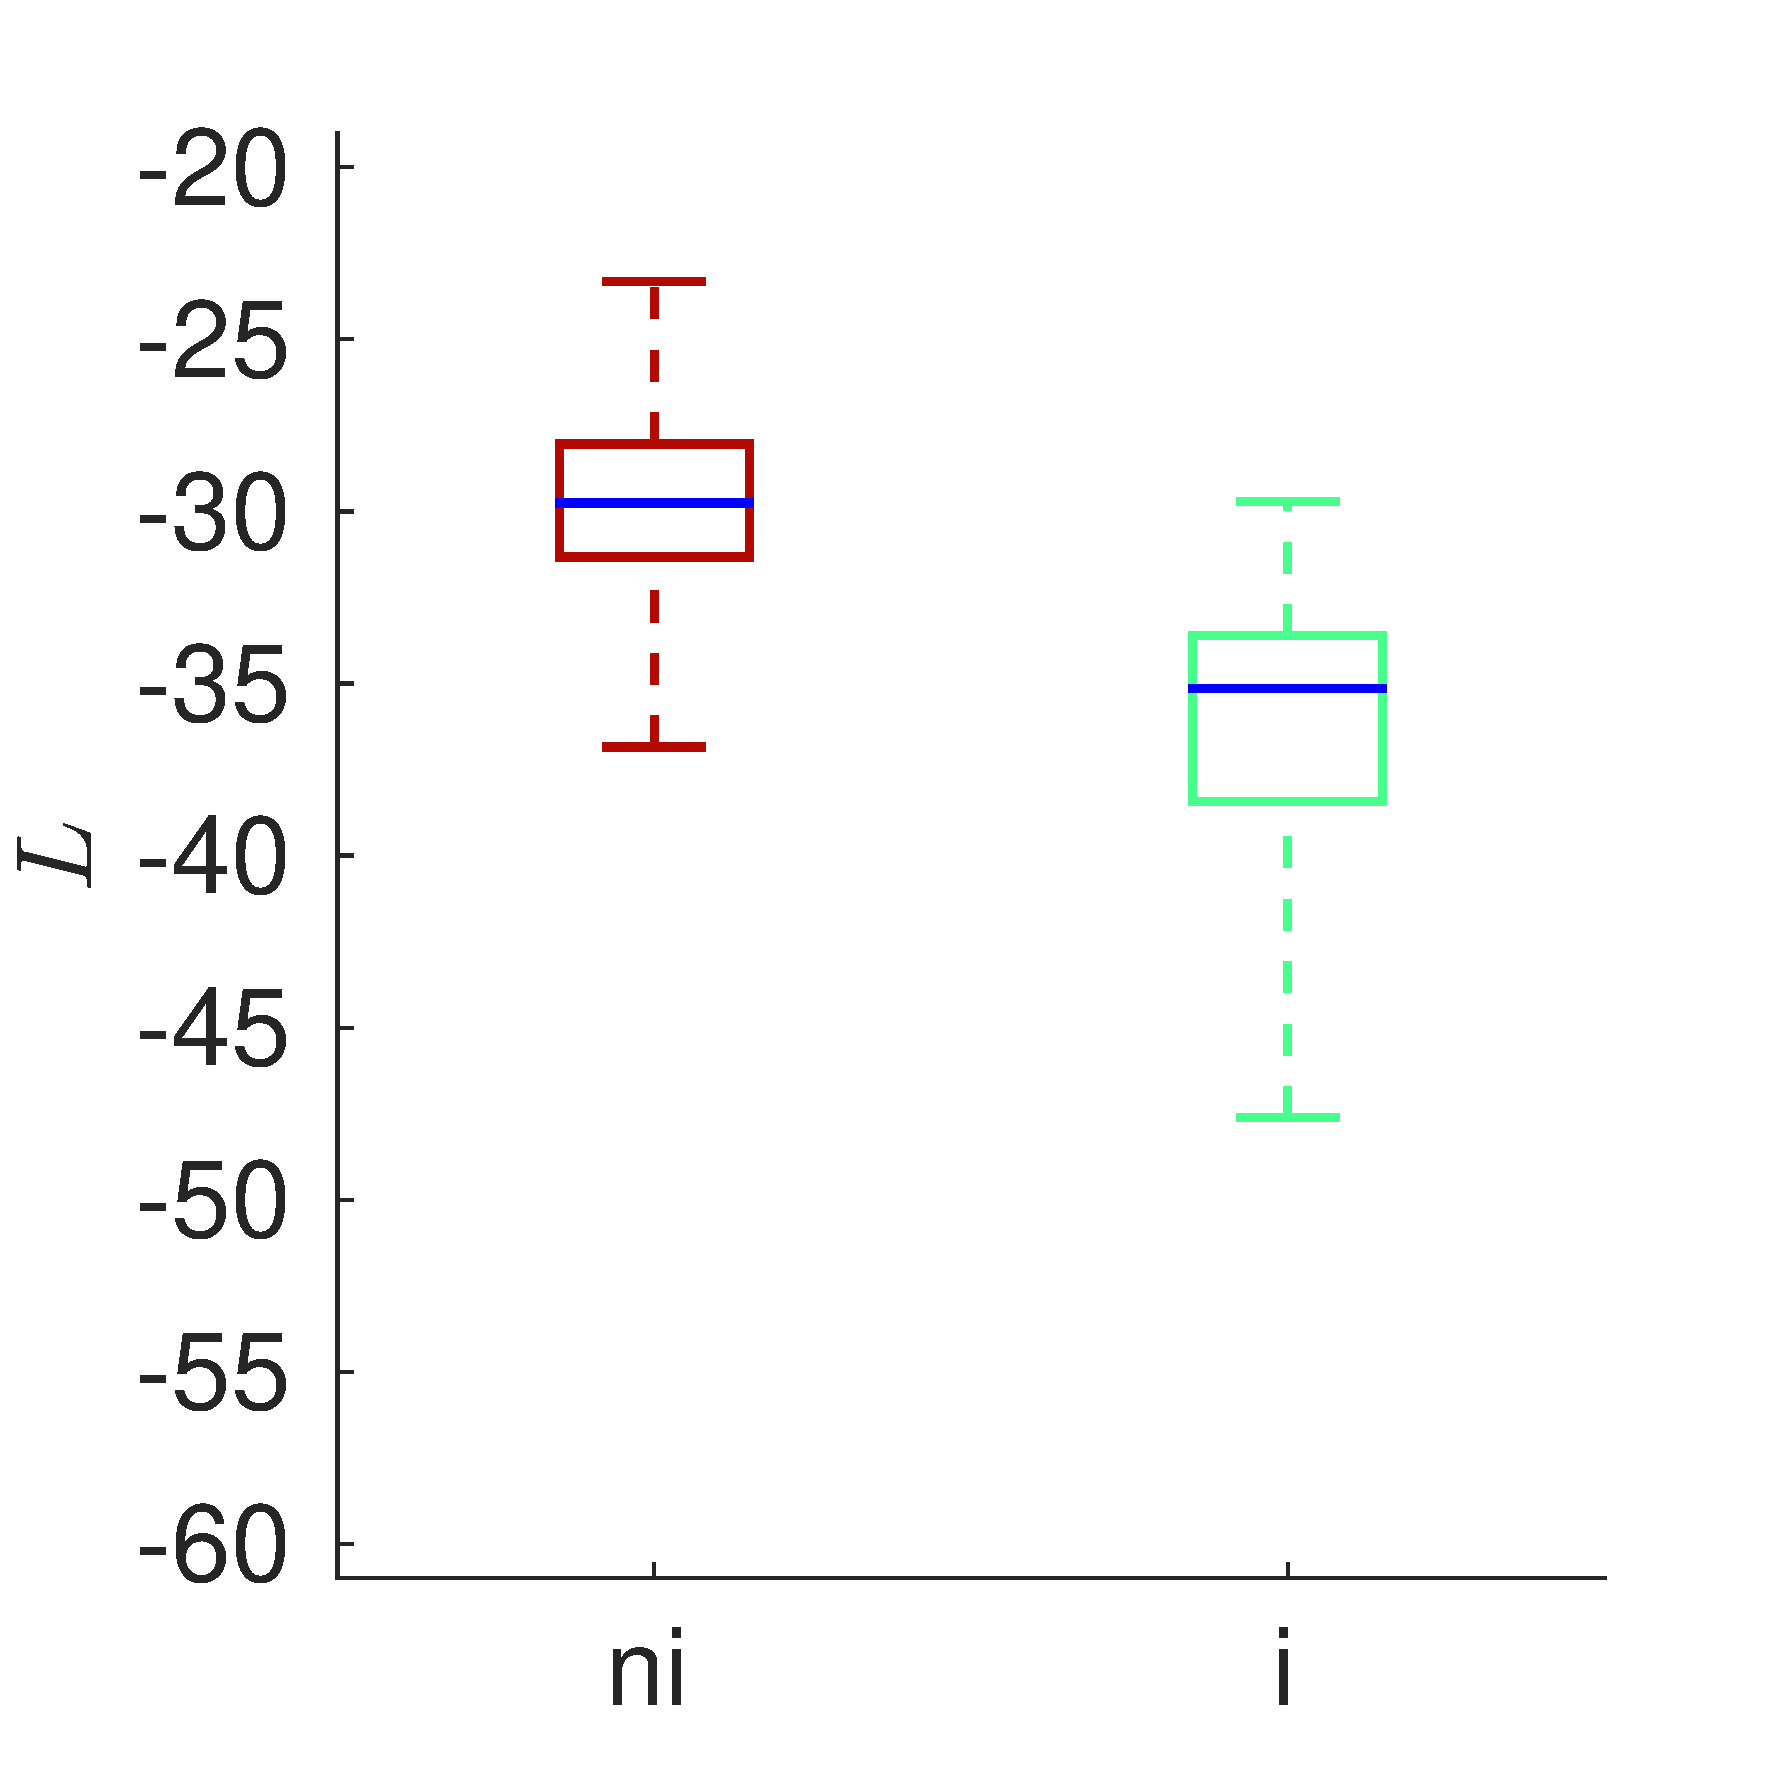
\includegraphics[width=.33\linewidth]{gfx/ch_5/xp_soundlevel_1}\label{fig:soundlevela}}
        \subfloat[]
        {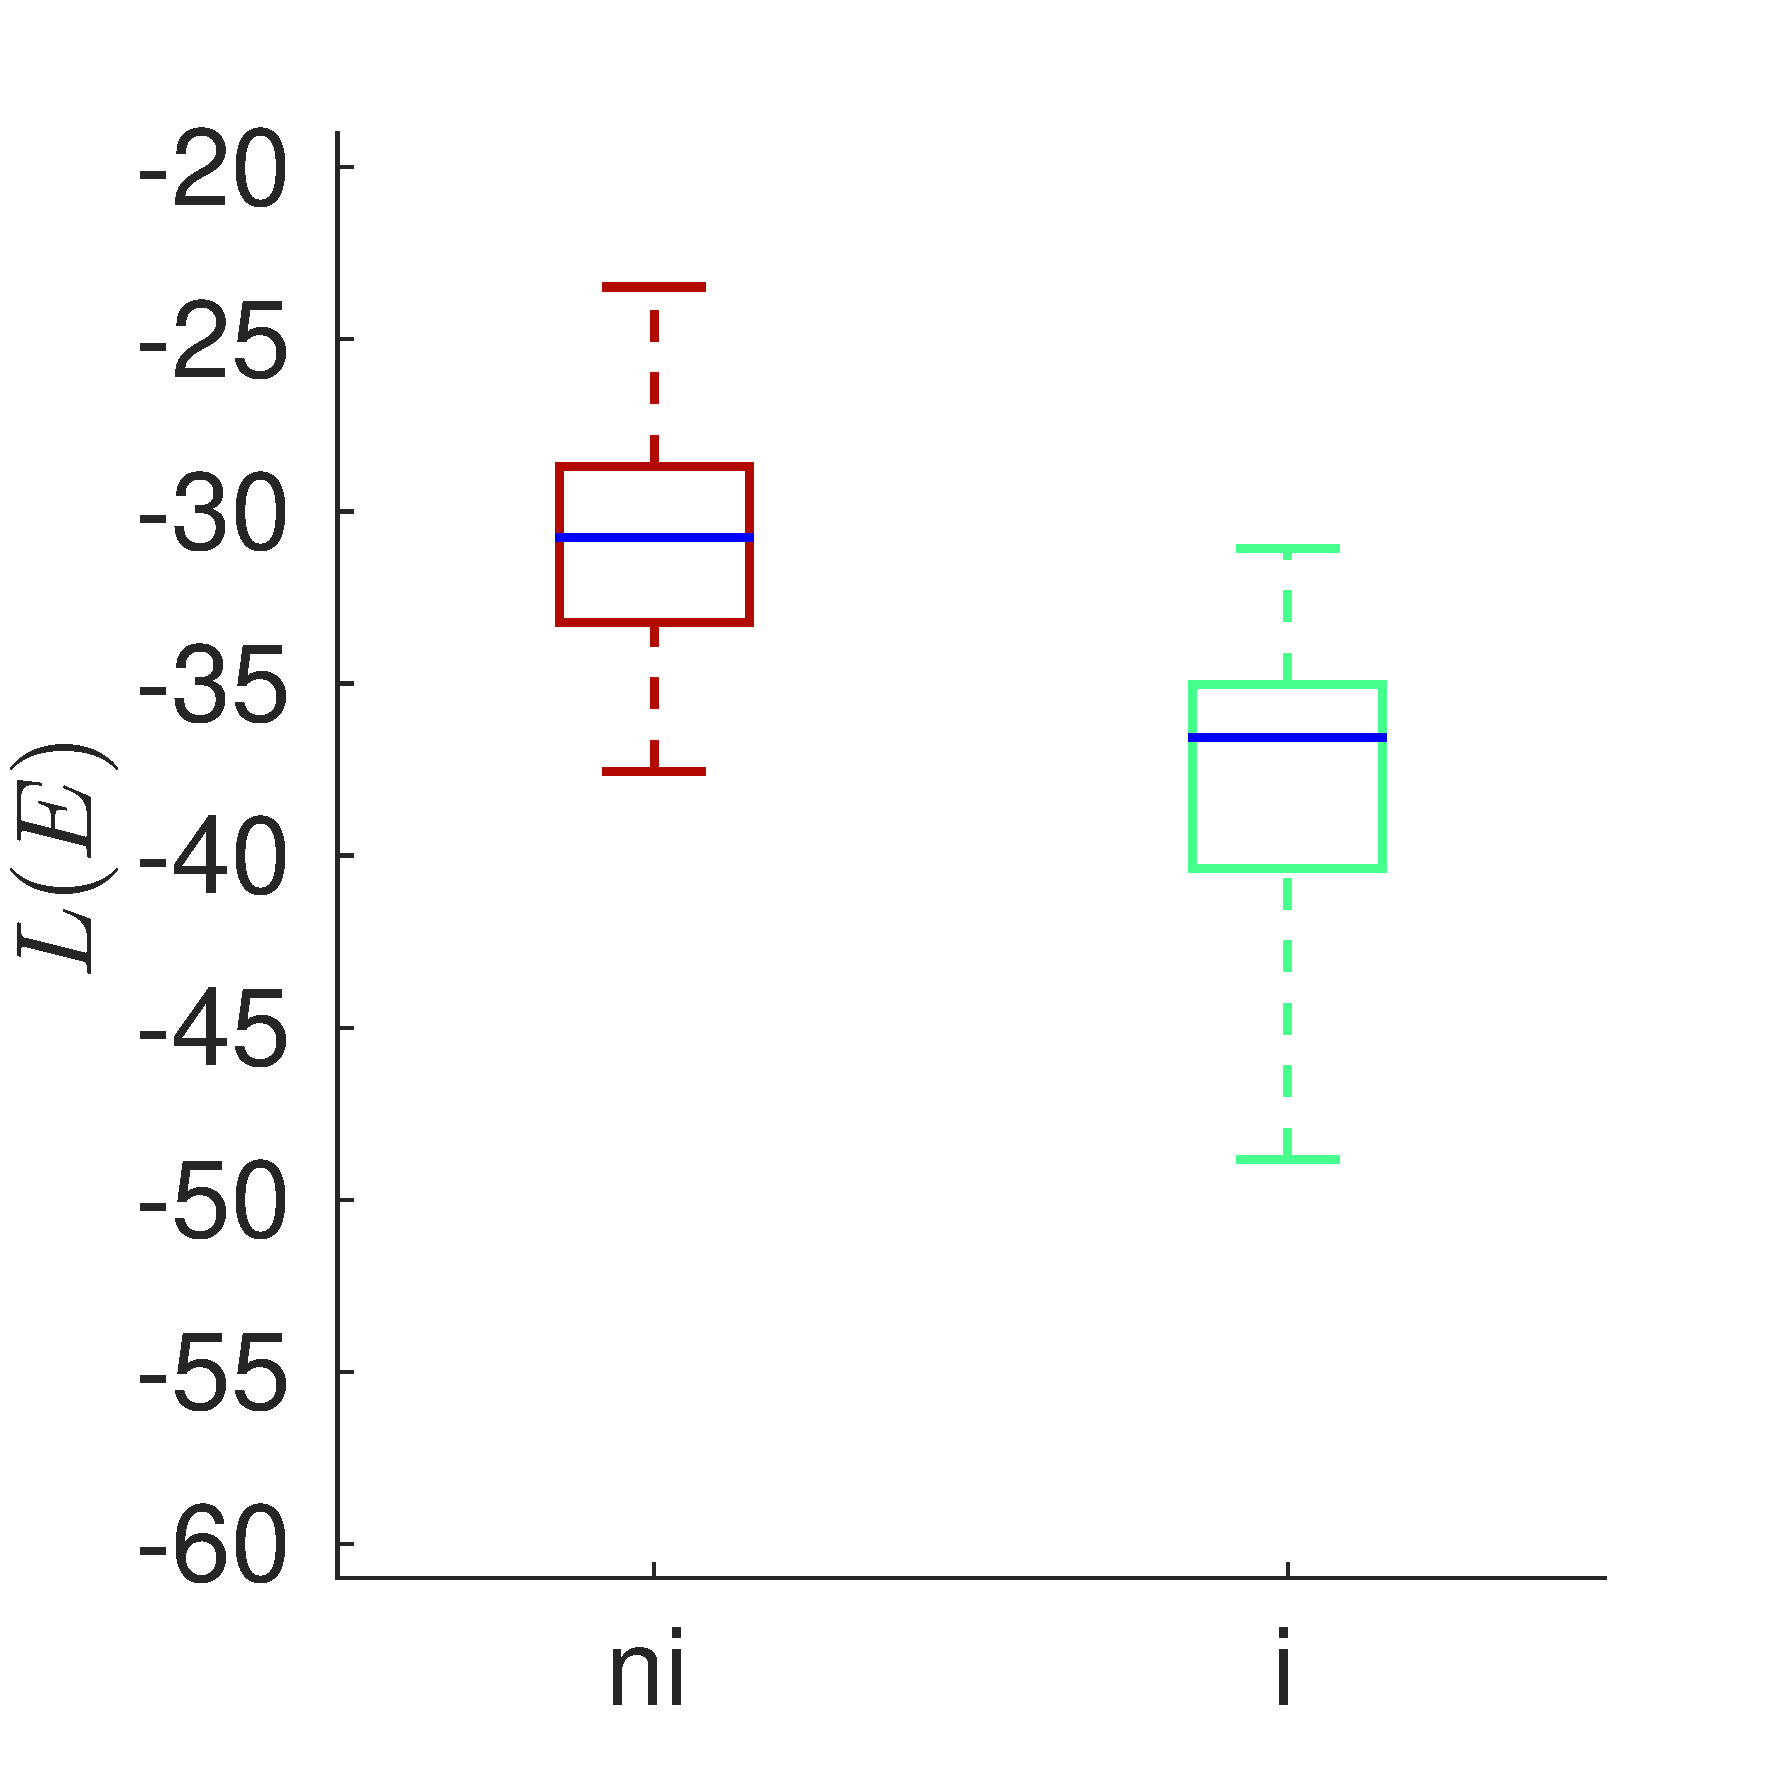
\includegraphics[width=.33\linewidth]{gfx/ch_5/xp_soundlevel_3}\label{fig:soundlevelb}}
        \subfloat[]
        {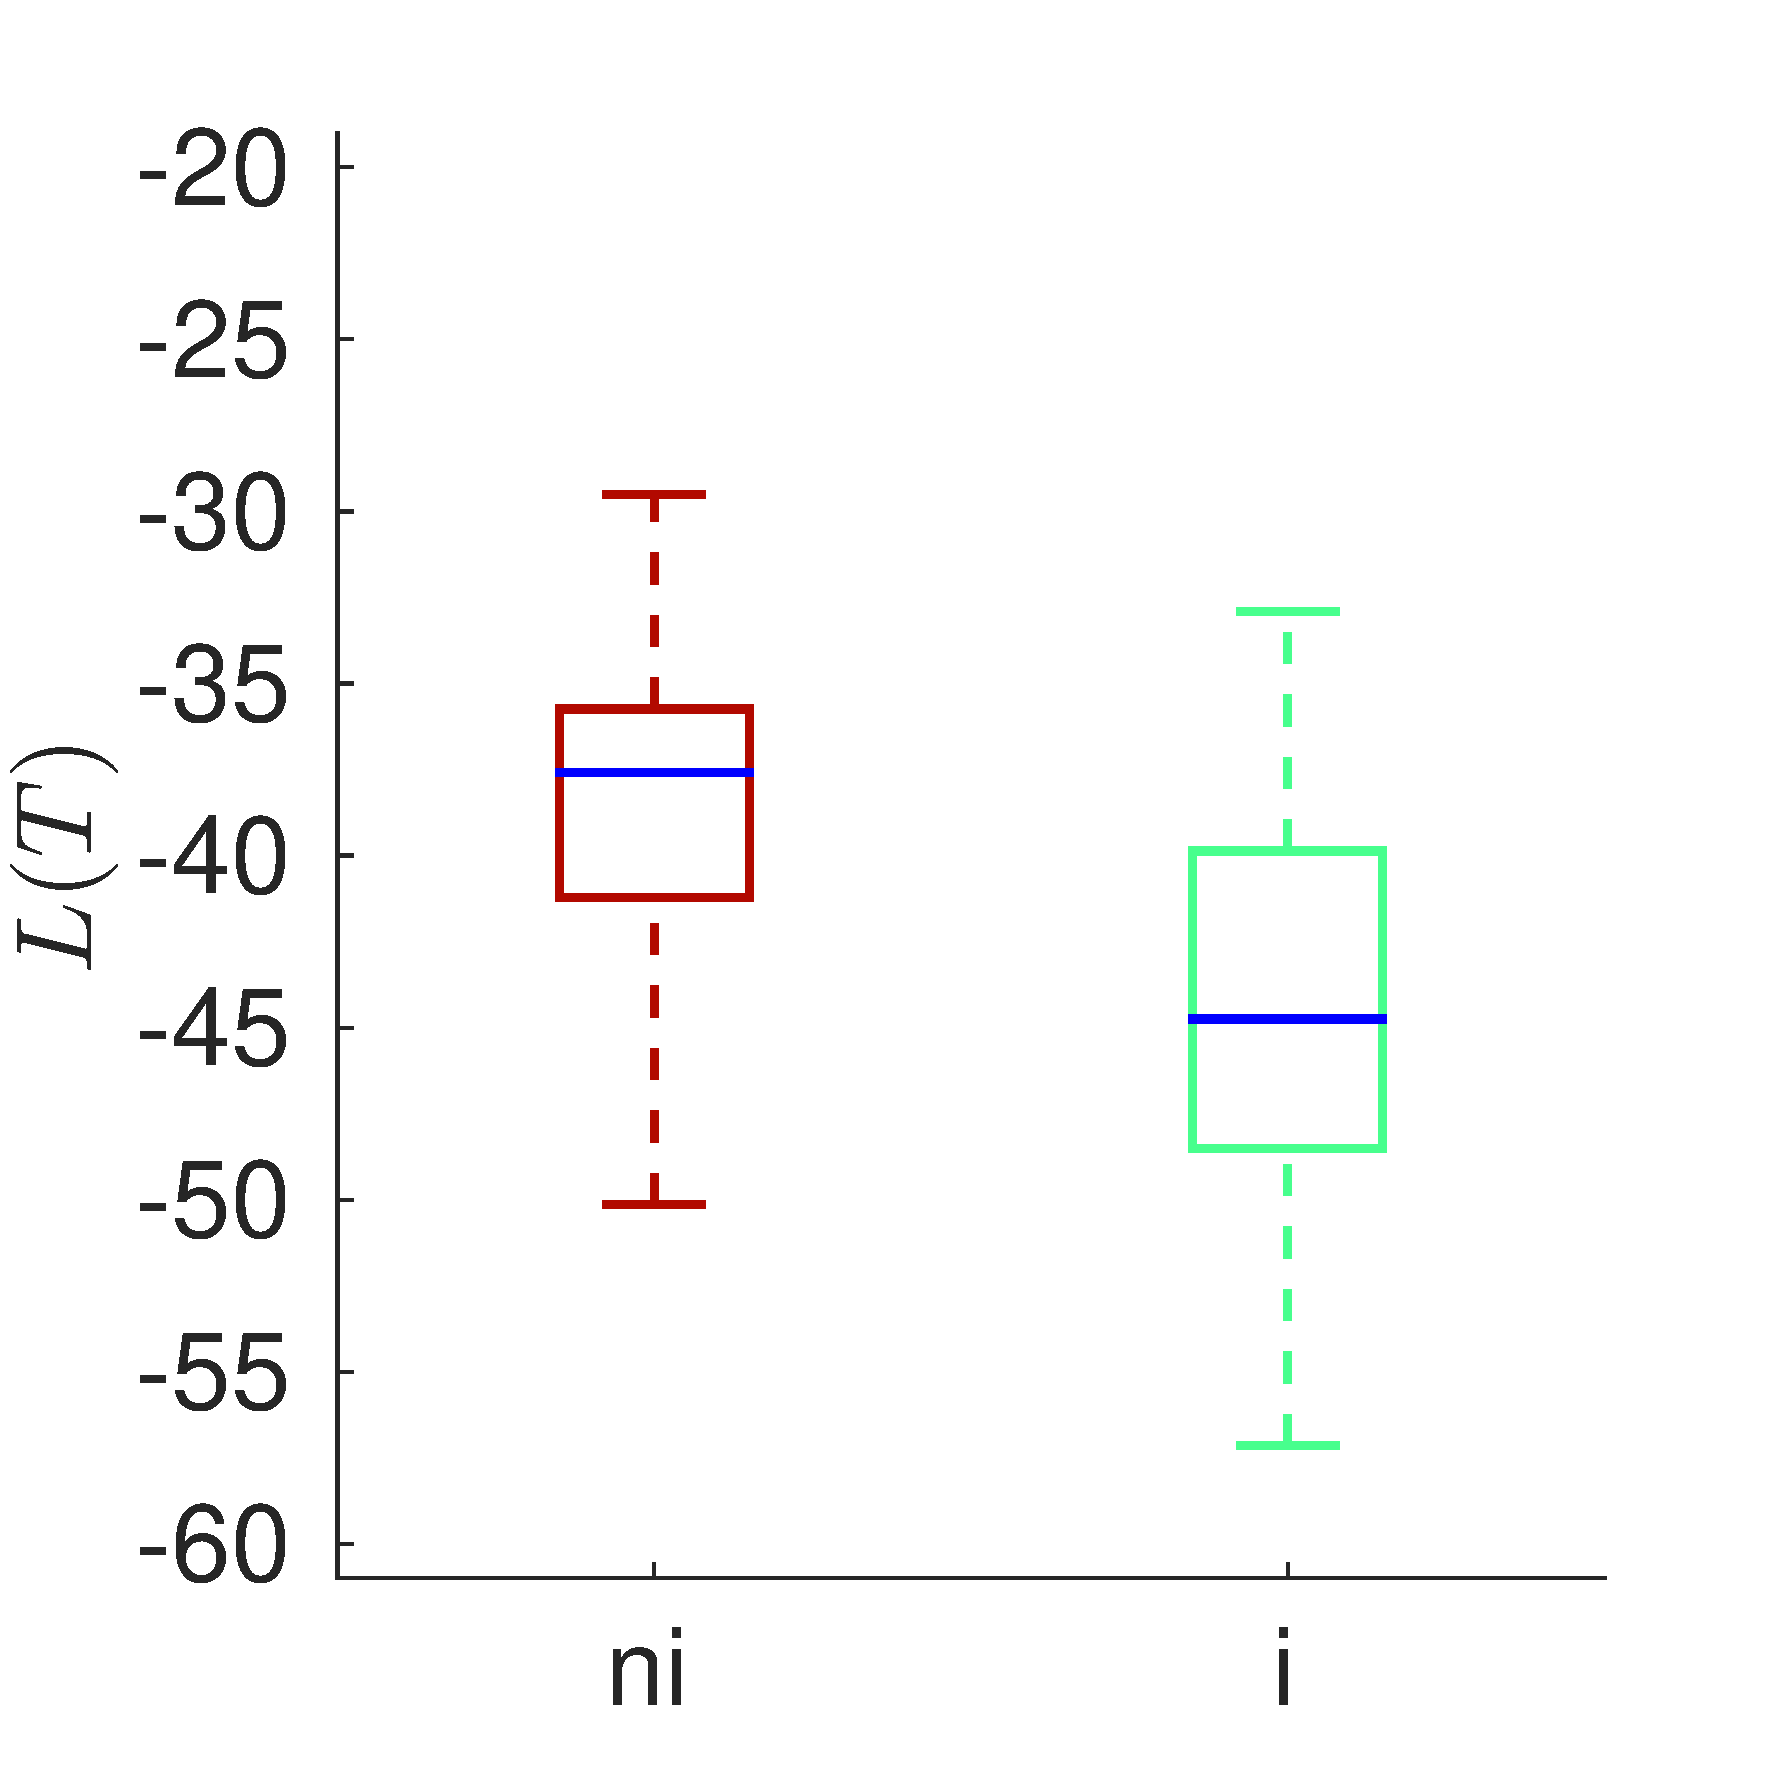
\includegraphics[width=.33\linewidth]{gfx/ch_5/xp_soundlevel_5}\label{fig:soundlevelc}}\par
        \subfloat[]
        {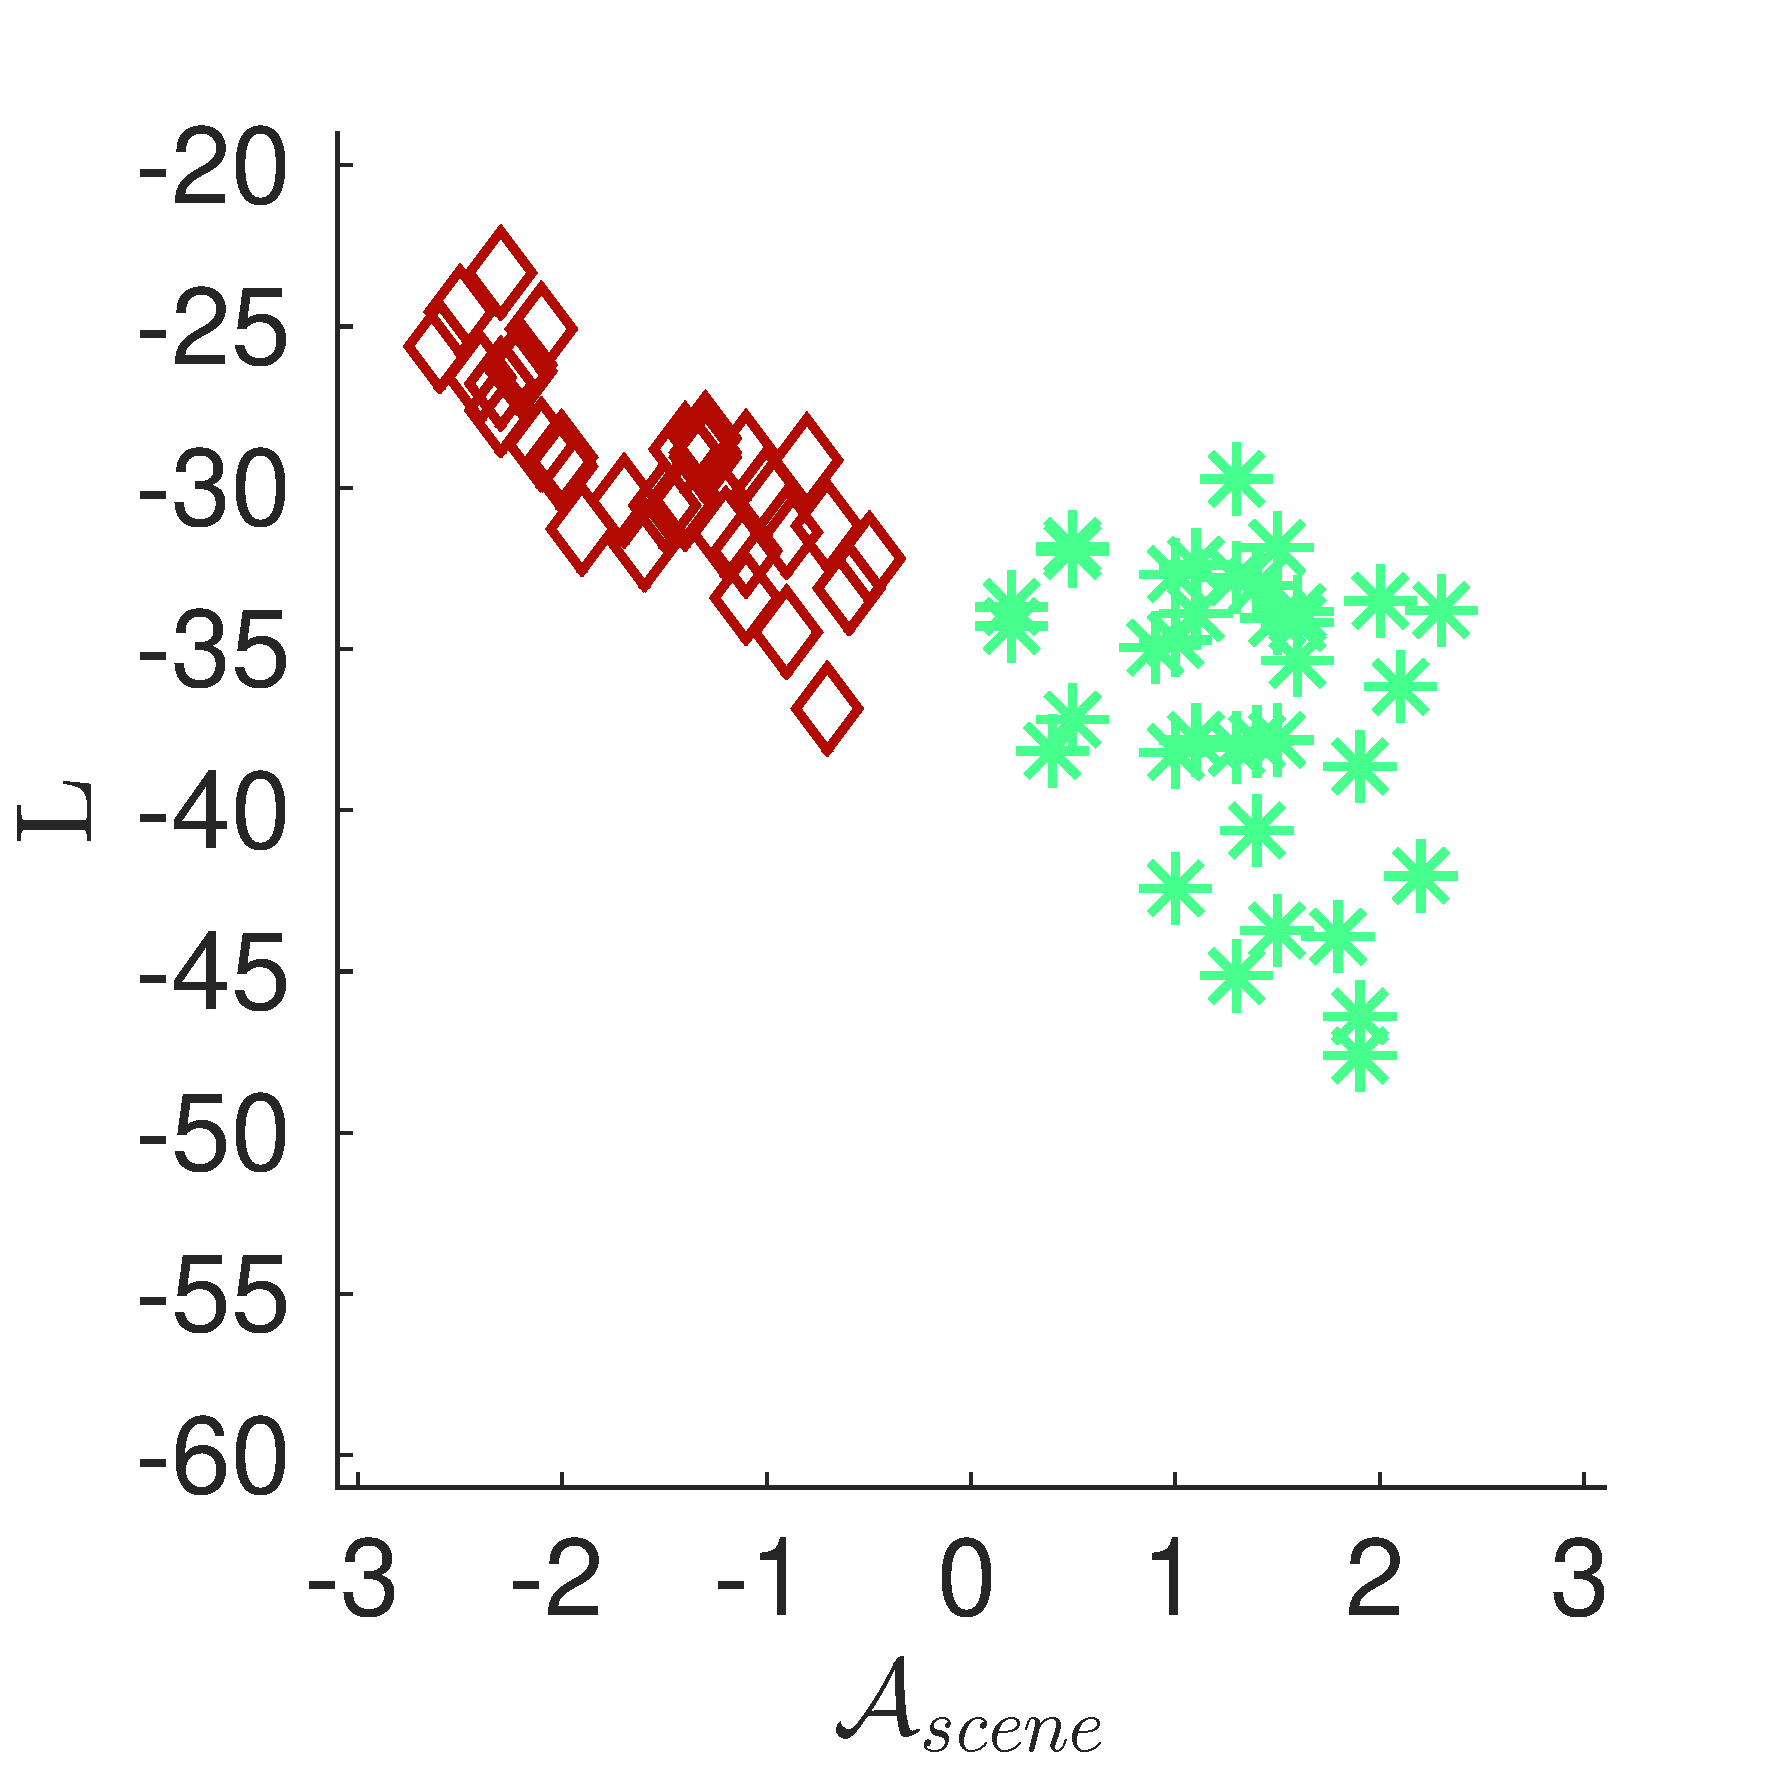
\includegraphics[width=.33\linewidth]{gfx/ch_5/xp_soundlevel_2}\label{fig:soundleveld}}
        \subfloat[]
        {\includegraphics[width=.33\linewidth]{gfx/ch_5/xp_soundlevel_4}\label{fig:soundlevele}}
        \subfloat[]
        {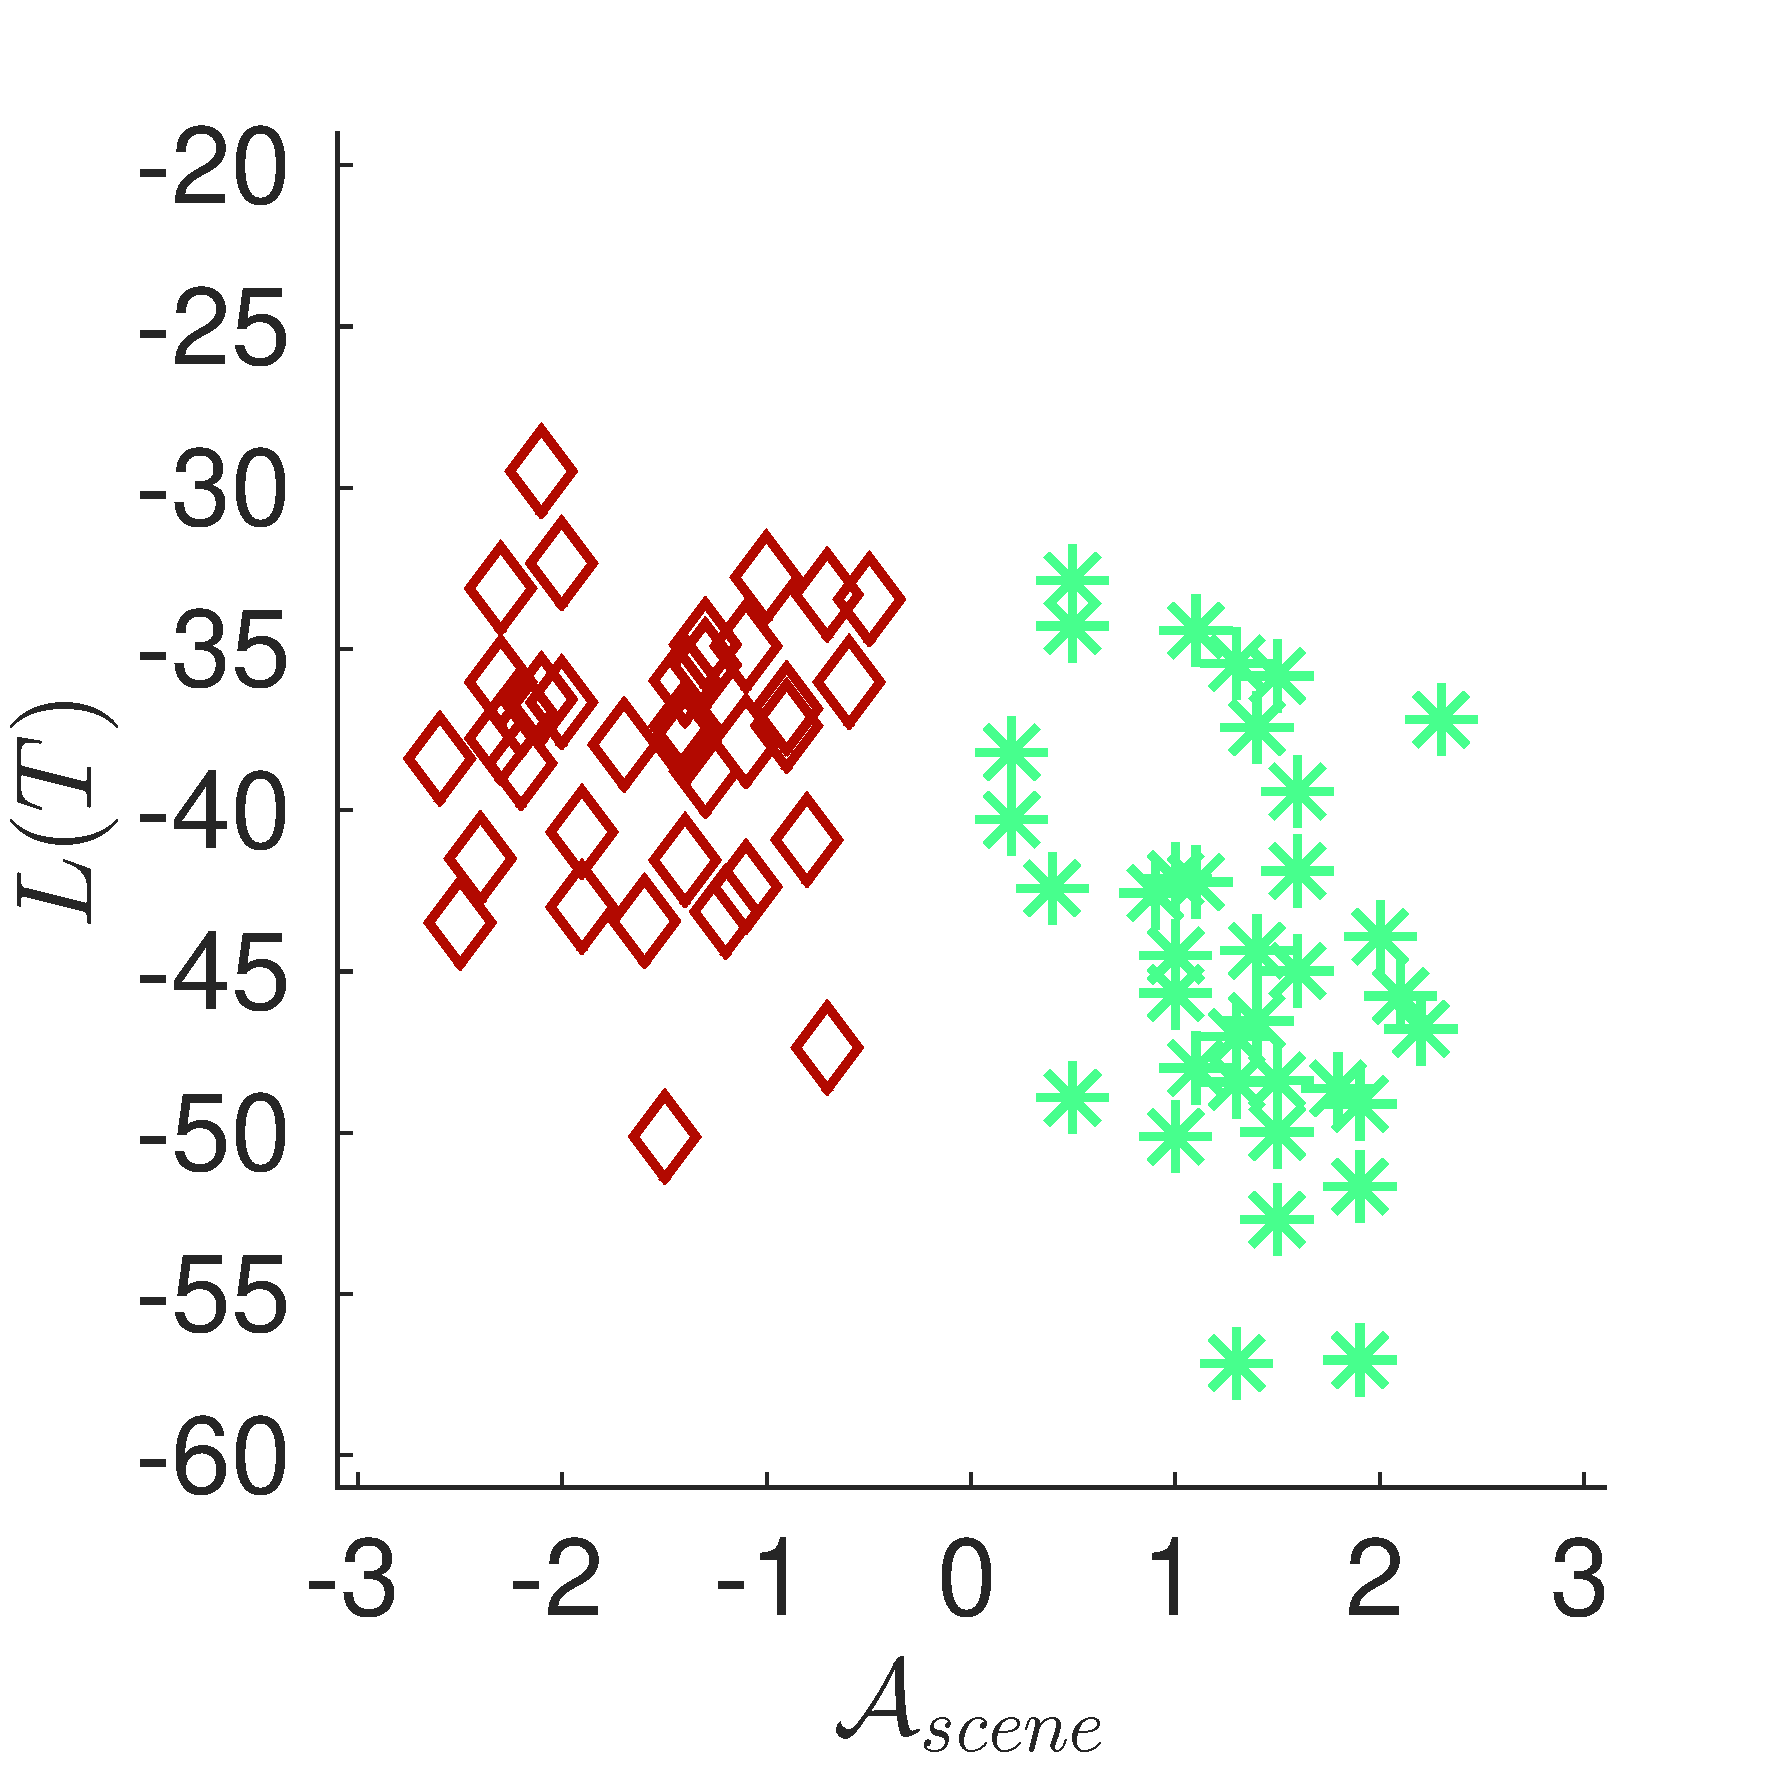
\includegraphics[width=.33\linewidth]{gfx/ch_5/xp_soundlevel_6}\label{fig:soundlevelf}}
       \caption{Dispersions des descripteurs structurels de niveaux sonores $L$ (a, d), $L(E)$ (b, e) et $L(T)$ (c, f), en fonction du type de scènes (a, b, c) et de l'agrément perçu $\mathcal{A}_{scene}$ de l'expérience 1.b (d, e, f).}\label{fig:soundlevel}
\end{figure}


\begin{figure}[t]
        \myfloatalign
        \subfloat[]
        {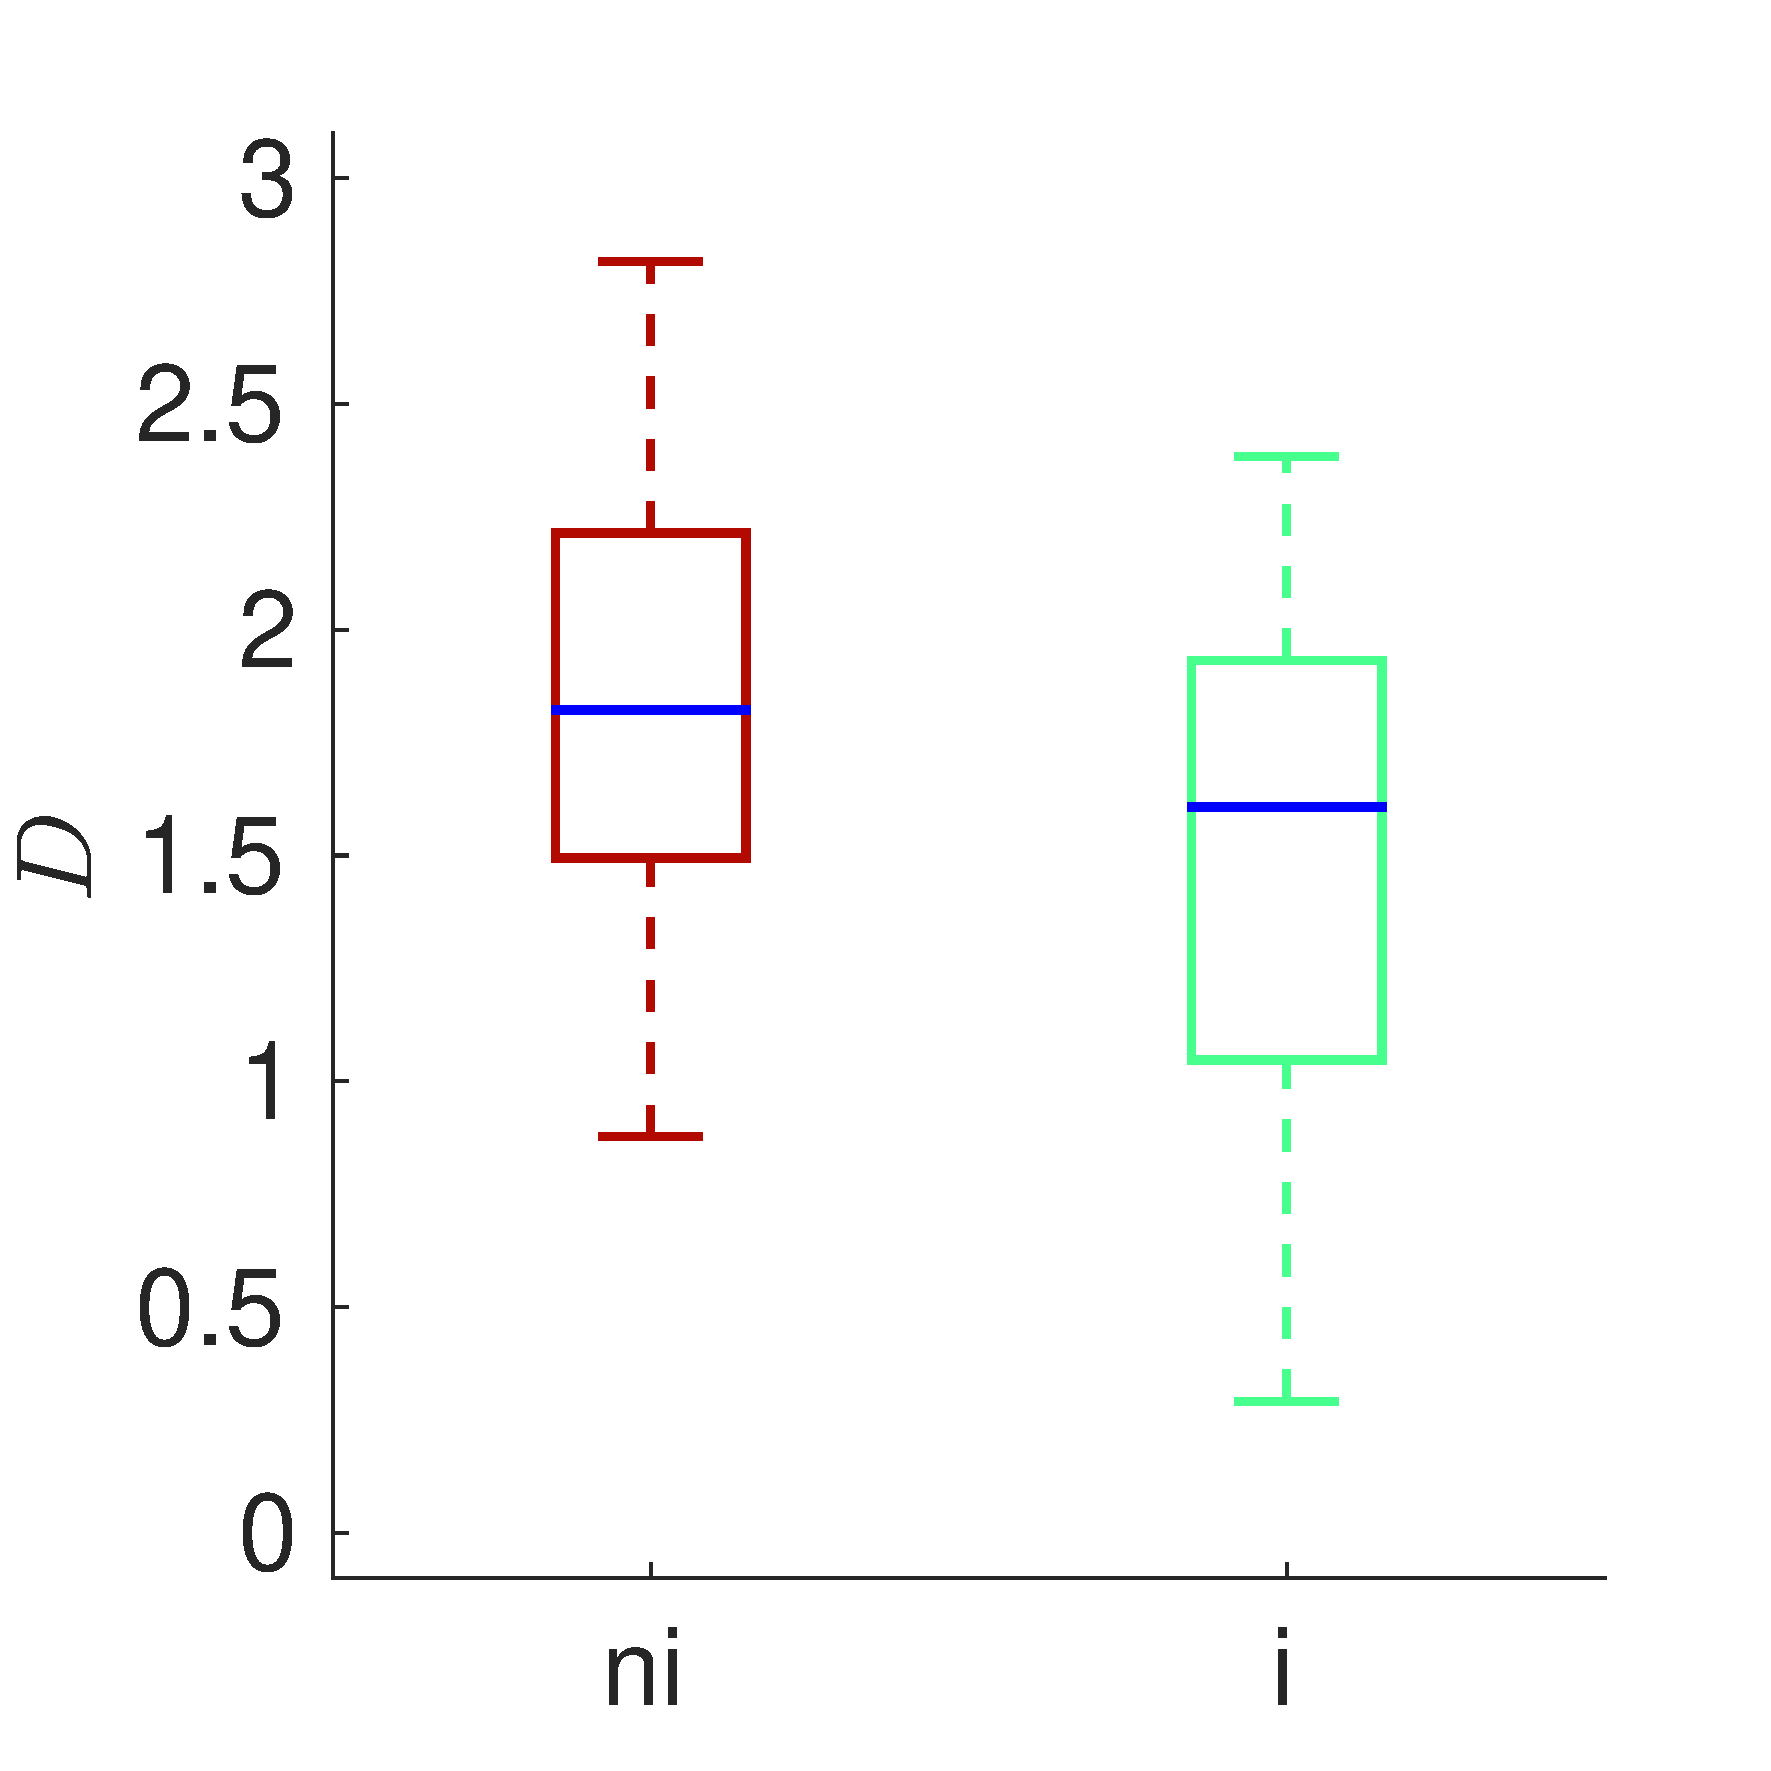
\includegraphics[width=.33\linewidth]{gfx/ch_5/xp_density_1}\label{fig:densitya}}
        \subfloat[]
        {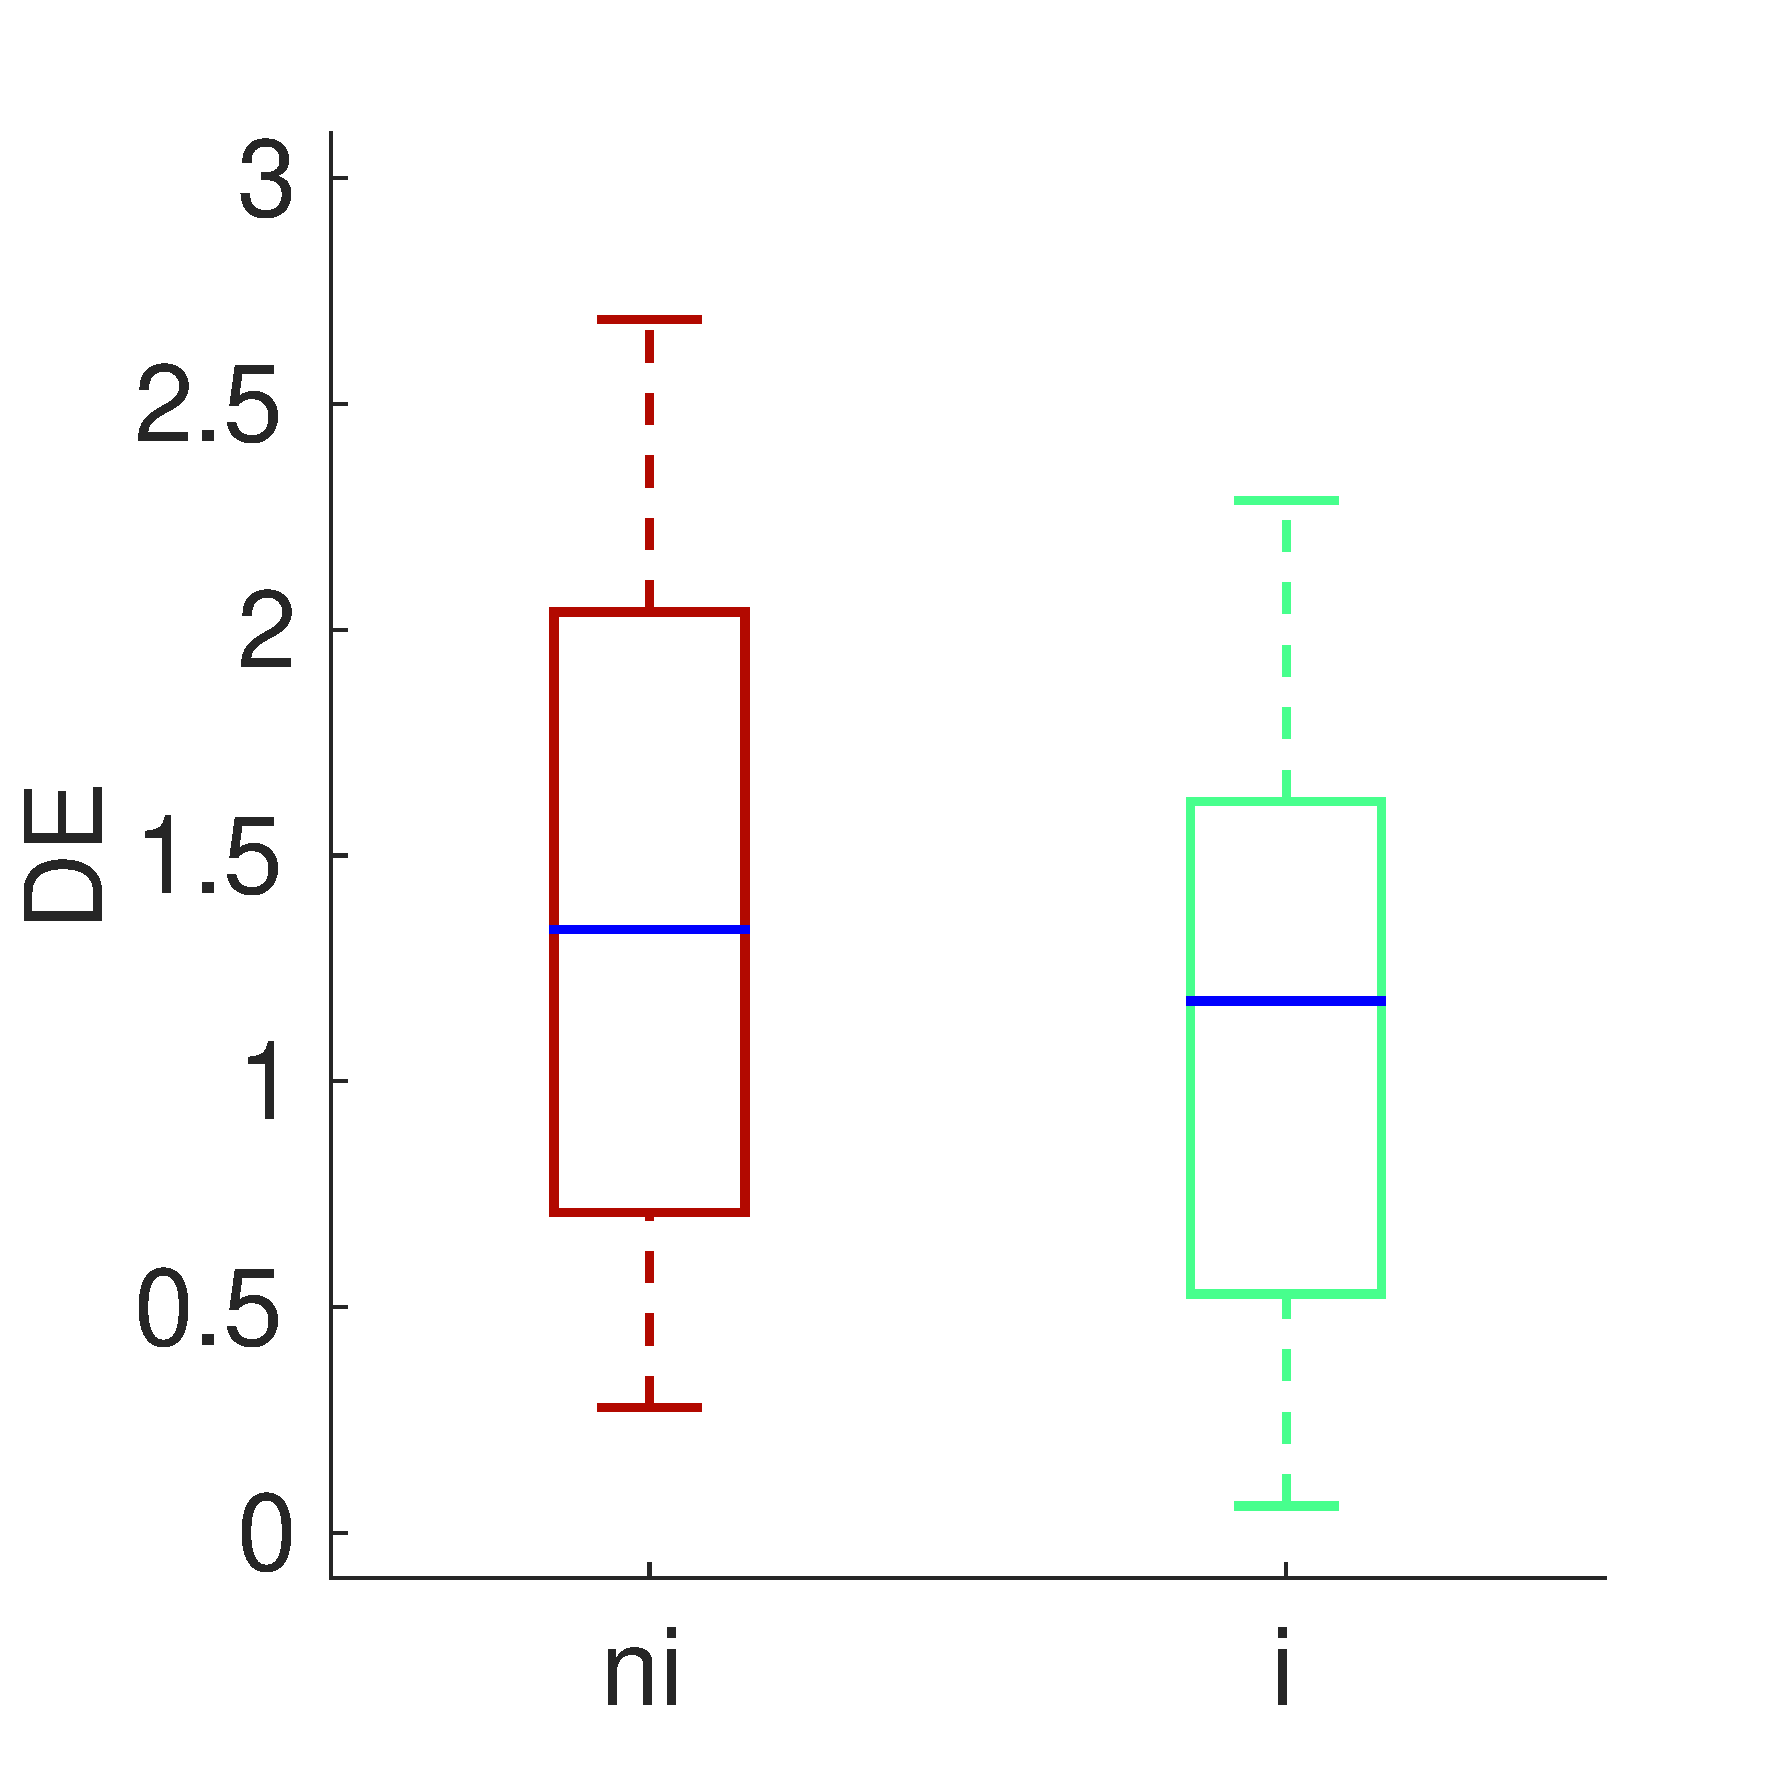
\includegraphics[width=.33\linewidth]{gfx/ch_5/xp_density_3}\label{fig:densityb}}\par
        \subfloat[]
        {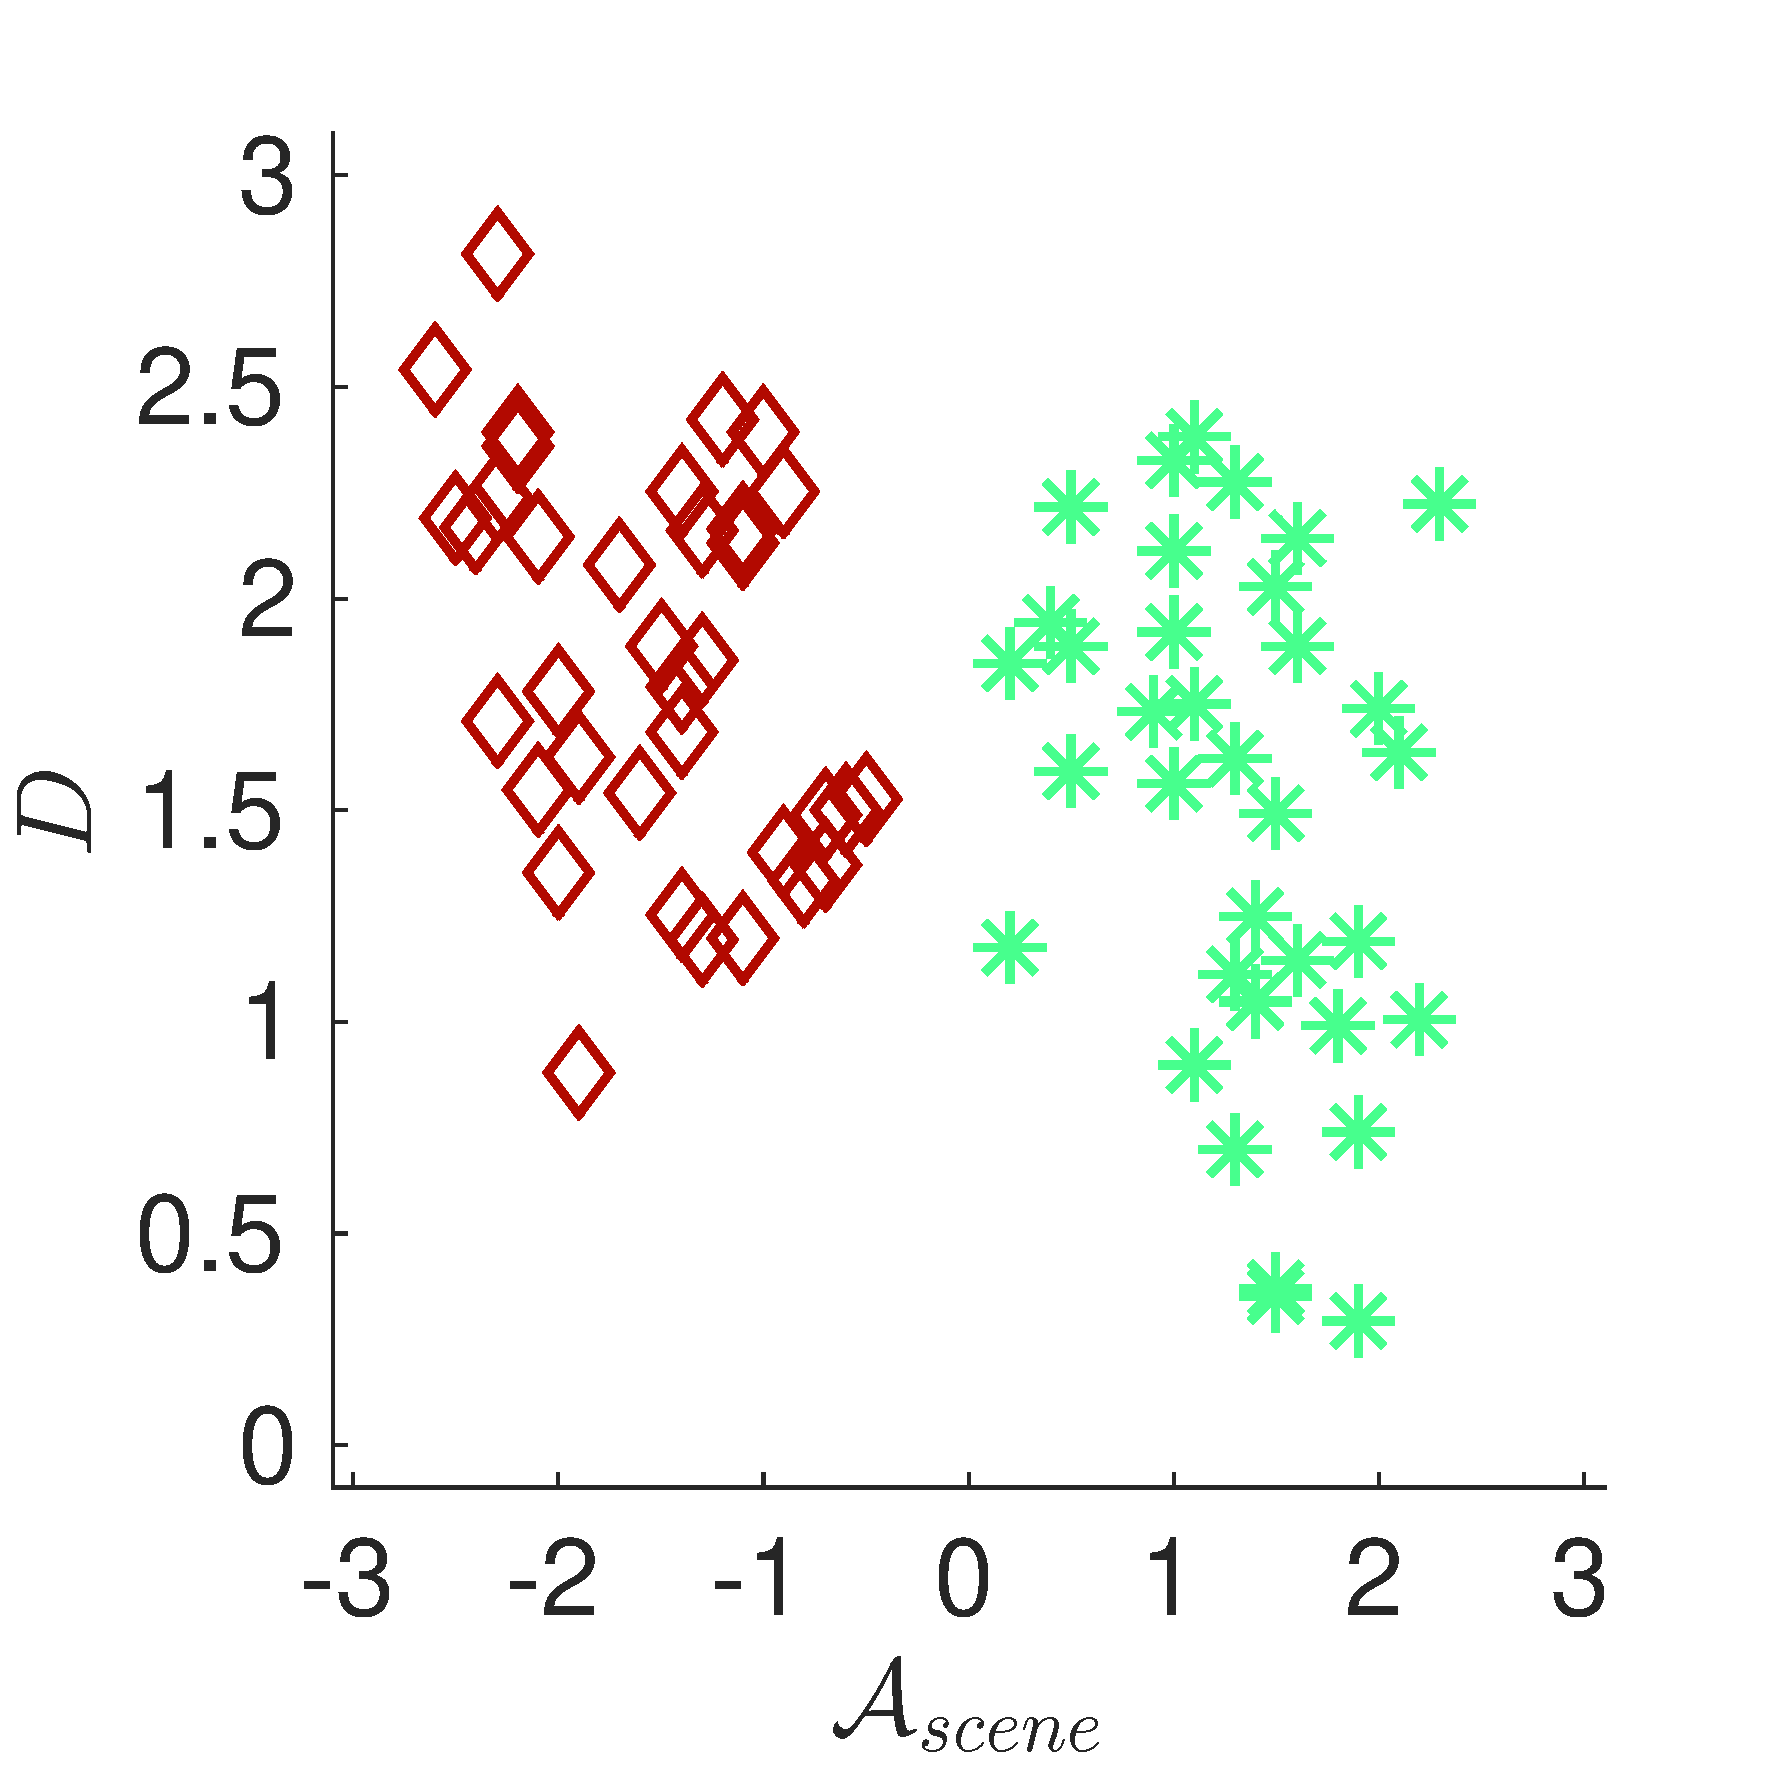
\includegraphics[width=.33\linewidth]{gfx/ch_5/xp_density_2}\label{fig:densityc}}
        \subfloat[]
        {\includegraphics[width=.33\linewidth]{gfx/ch_5/xp_density_4}\label{fig:densityd}}
       \caption{Dispersions des descripteurs structurels de densité $D$ (a, c) et $D(E)$ (b, d), en fonction du type de scènes (a, b) et de l'agrément perçu $\mathcal{A}_{scene}$ de l'expérience 1.b (c, d).}\label{fig:density}
\end{figure}

\begin{figure}[t]
        \myfloatalign
        \includegraphics[width=.8\linewidth]{gfx/ch_5/xp1_div_1}
       \caption{Moyenne et écart type de la diversité des classes utilisées en considérant l'ensemble des classes ($DIV$), les classes d'événements ($DIV(E)$) et les classes de textures ($DIV(T)$), en considérant séparément les i- et ni-scènes ainsi que les différents niveaux d'abstraction.}\label{fig:diversity}
\end{figure}

\subsection{Influence des descripteurs structurels sur l'agrément perçu}
\label{sec:ch5_corrDesStruct}

Dans cette partie nous analysons les relations fines qui peuvent exister entre les descripteurs structurels, d'une part, et l'agrément perçu, d'autre part. Contrairement à la section précédente, où la qualité affective des scènes est représentée de manière binaire (i \vs~ni), nous considérons, ici, l'agrément moyen $\mathcal{A}_{scene}$ comme descripteur perceptif. Il s'agit d'étudier l'existence de potentielles corrélations entre les descripteurs structurels et $\mathcal{A}_{scene}$. Les coefficients de corrélations linéaires calculés entre $\mathcal{A}_{scene}$ \vs~$L$, $L(E)$, $L(T)$, $D$, $D(E)$ et $DIV(E)$ sont présentés dans le tableau~\ref{tab:corrStructA}. Les relations entre $\mathcal{A}_{scene}$ et les descripteurs structurels sont illustrées par les figures~\ref{fig:soundleveld},~\ref{fig:soundlevele} et ~\ref{fig:soundlevelf}, pour les niveaux sonores, et les figures~\ref{fig:densityc} et~\ref{fig:densityd}, pour les densités. 

Concernant $L$, on observe une forte corrélation négative ($r=-0.77$, $p<0.01$) avec $\mathcal{A}_{scene}$, indiquant que plus le niveau sonore est élevé, plus la scène est désagréable. Cependant, la figure~\ref{fig:soundleveld} suggère que cette relation ne s'opère pas de la même manière pour les i- et ni-scènes. En effet, la corrélation entre $L$ et $\mathcal{A}_{scene}$, pour les ni-scènes, reste élevée ($r=-0.78$, $p<0.01$), mais est inexistante pour les i-scènes. 

Cette corrélation élevée, considérant l'ensemble des scènes, résulte du fait que les i-scènes ont tendance à être moins fortes que les ni-scènes, donnant ainsi l'illusion de prolonger la corrélation négative observée pour les ni-scènes.  

Nous en concluons que $L$:

\begin{itemize}
\item permet bien de faire la distinction entre les i- et ni-scènes,
\item permet de finement caractériser l'agrément perçu des ni-scènes,
\item n'est pas un indicateur pertinent de l'agrément perçu pour des environnements a priori agréables.
\end{itemize}

Les mêmes observations sont faites concernant $L(E)$ (\cf~\ref{fig:soundlevele}). Pour $L(T)$ (\cf~\ref{fig:soundlevelf}), bien que, à considérer l'ensemble des scènes, on observe une corrélation modérée, cela n'est pas vérifié quand on regarde séparément les i-scènes ($r=-0.33$, $p=0.05$) et les ni-scènes ($r=-0.00$, $p=0.99$). Là encore on peut penser que la corrélation négative observée pour l'ensemble des scènes est un artefact, résultant du fait que le niveau des textures des i-scènes a tendance à être plus bas que celui des ni-scènes. Ainsi, si les événements sonores conservent une certaine capacité de prédiction de l'agrément pour les ni-scènes, le niveau des textures n'apporte, lui, que peu d'informations, quel que soit l'environnement.

Considérant l'ensemble des scènes, nous observons une corrélation négative faible pour $D$ ($r=-0.43$, $p<0.01$) et $D(E)$ ($r=-0.34$, $p<0.01$). Une relation semblable est observée pour les ni-scènes ($D$: $r=-0.38$, $p<0.05$; $D(E)$: $r=-0.46$, $p<0.01$), mais aucune corrélation n'est observée pour les i-scènes. La densité de sources sonores semble donc avoir un faible impact sur l'agrément perçu, si l'on considère les ni-scènes, mais, comme pour les niveaux, cette densité ne semble pas avoir d'impact pour les i-scènes.

En ce qui concerne la diversité des classes d'événements, une corrélation négative faible est observée pour les niveaux d'abstraction 1, 2 et 3, en tenant compte de l'ensemble des scènes. Si l'on considère les i- et ni-scènes séparément, aucune corrélation significative n'est trouvée. Les conclusions sont similaires à celles faites pour $L(T)$: la diversité permet uniquement de faire la distinction entre les deux types d'environnements, mais ne permet pas de caractériser précisément l'agrément perçu.

En résumé, en présence d'un environnement désagréable, les niveaux sonores, en particulier ceux des événements, ainsi que, dans une moindre mesure, la densité de sources présentes, ont un impact négatif sur l'agrément. En présence d'un environnement agréable, en revanche, aucun des descripteurs structurels considérés ici ne semble influer sur la perception de l'agrément. 

Ces premiers résultats pourraient montrer qu'il existe deux modes de perception, mobilisant chacun des descripteurs indépendants, modes qui s'activent en fonction de la nature de l'environnement (i ou ni).

Le fait qu'aucun des descripteurs globaux ne permettent de caractériser l'agrément des i-scènes peut nous amener à penser que toutes les sources sonores ne contribuent pas de manière égale à la perception de l'agrément, mais, que seules les caractéristiques de certaines d'entre elles ont une réelle influence. Afin d'approfondir ce point, nous analysons, dans la section suivante, les scènes d'un point de vue sémantique, \ie~en nous intéressant à la nature des sources qui les composent. \\


\begin{table}[t]
\centering
\begin{tabular}{l c c c} 
               & ensemble                     & i-scènes                   & ni-scènes    \\
\hline
$L$            & \textbf{-0.77} ($p<0.01$)    & -0.32 ($p=0.06$)           & \textbf{-0.78} ($p<0.01$)\\
$L(E)$         & \textbf{-0.75} ($p<0.01$)    & -0.20 ($p=0.24$)           & \textbf{-0.75} ($p<0.01$)\\
$L(T)$         & \textbf{-0.53} ($p<0.01$)    & -0.33 ($p=0.05$)           &  -0.00 ($p=0.99$) \\
$D$            & \textbf{-0.43} ($p<0.01$)    & -0.31 ($p=0.07$)           & \textbf{-0.38} ($p<0.05$)\\
$D(E)$         & \textbf{-0.34} ($p<0.01$)    & -0.22 ($p=0.21$)           & \textbf{-0.46} ($p<0.01$)\\
$DIV(E)$ 0     &          -0.07 ($p=0.52$)    & -0.25 ($p=0.15$)           & -0.23 ($p=0.23$)\\
$DIV(E)$ 1     & \textbf{-0.47} ($p<0.01$)    & -0.25 ($p=0.14$)           & -0.26 ($p=0.13$)\\
$DIV(E)$ 2     & \textbf{-0.41} ($p<0.01$)    & -0.21 ($p=0.22$)           & -0.25 ($p=0.14$)\\
$DIV(E)$ 3     & \textbf{-0.37} ($p<0.01$)    & -0.18 ($p=0.30$)           & -0.18 ($p=0.16$)\\
\hline
\end{tabular}
\vspace{0.5mm}
\caption{Coefficients de corrélation linéaire calculés entre l'agrément perçu moyen $\mathcal{A}_{scene}$ de l'expérience 1.b et les descripteurs structurels.}
\label{tab:corrStructA}
\end{table}

\subsection{Étude comparative entre les descripteurs sémantiques}

\subsubsection{Analyse qualitative}
\label{sec:ch5_anaQualiSem}

Nous analysons la composition des scènes en comptant le nombre de sujets ayant utilisé une classe de sons pour simuler un type d'environnement. Les résultats sont présentés à la figure~\ref{fig:soundsourcea} pour les événements, et à la figure~\ref{fig:soundsourceb} pour les textures. Par souci d'espace, nous choisissons un niveau d'abstraction intermédiaire entre le niveau 0 et 1, noté $0+$, pour représenter les classes (\cf~Figure~\ref{fig:taxonomie}).

Nous observons une différence notable dans le choix des classes entre les i- et ni-scènes. La répartition des classes est très proche de celle obtenue dans une étude similaire sur les environnements sonores urbains idéaux \citep{guastavino2006ideal}, \ie~les classes suggérant la présence humaine et la nature sont très présentes dans les i-scènes, a contrario, les classes désignant des sons mécaniques et/ou de travaux sont principalement utilisées pour les ni-scènes.

Ces résultats confirment un fait déjà observé: la nature sémantique des sources sonores joue un rôle prédominant dans l'appréciation de l'environnement \citep{raimbault2005urban,dubois2006cognitive}.

Nous notons quelques différences avec \citep{guastavino2006ideal}: les résultats obtenus par Guastavino montrent que les sons de \emph{transports publics} sont caractéristiques des environnements sonores urbains idéaux. Les auteurs attribuent cela au fait que la perception de l'agrément est, entre autre, soumise à un contexte socio-culturel. Dans notre représentation du monde, les sons de transports publics sont positivement connotés, et ont ainsi tendance à être mieux acceptés que les sons de véhicules privés.

Dans une certaine mesure, nos résultats contredisent ce fait. La figure~\ref{fig:soundsourcea} montre, en effet, que les classes d'événements de \emph{transports publics} (\emph{bus} et \emph{train}, \cf~Figure~\ref{fig:soundsourcec}) ont été utilisées par les sujets, pour des i-scènes, dans $28\%$ des cas, et pour des ni-scènes, dans $42\%$ des cas. Les résultats ne remettent pas en question le fait que les sons de \emph{transports publics} soient bien acceptés: $25\%$ des sujets ont utilisé la classe \emph{bus} pour les i-scènes, un chiffre comparable à celui de la classe \emph{Vélo}, et bien supérieur à celui de toute autre classe de véhicules privés. Cependant les classes \emph{transports publics} sont également bien présentes dans les ni-scènes, plus que les classes \emph{voiture} ou \emph{camion} par exemple. La classe \emph{transports publics} ne peut donc pas être considérée comme typique d'un environnement sonore urbain idéal.

Cette différence peut s'expliquer par la nature des deux protocoles expérimentaux utilisés. Comme nous l'avons fait, Guastavino demande à ses sujets de décrire un environnement en se basant sur leurs mémoires. Mais, contrairement à nous, ils ne disposent pas de supports sonores. Le fait que nos sujets soient confrontés à la réalité acoustique des sons, pour recréer leurs environnements, peut avoir pour effet de diminuer l'impact du contexte socio-culturel. D'autres études utilisant des sons comme stimuli montrent que la classe \emph{bus} peut avoir un effet négatif sur l'appréciation de l'environnement \citep{lavandier2006contribution}.

\begin{figure}[t]
        \myfloatalign
        \subfloat[]
        {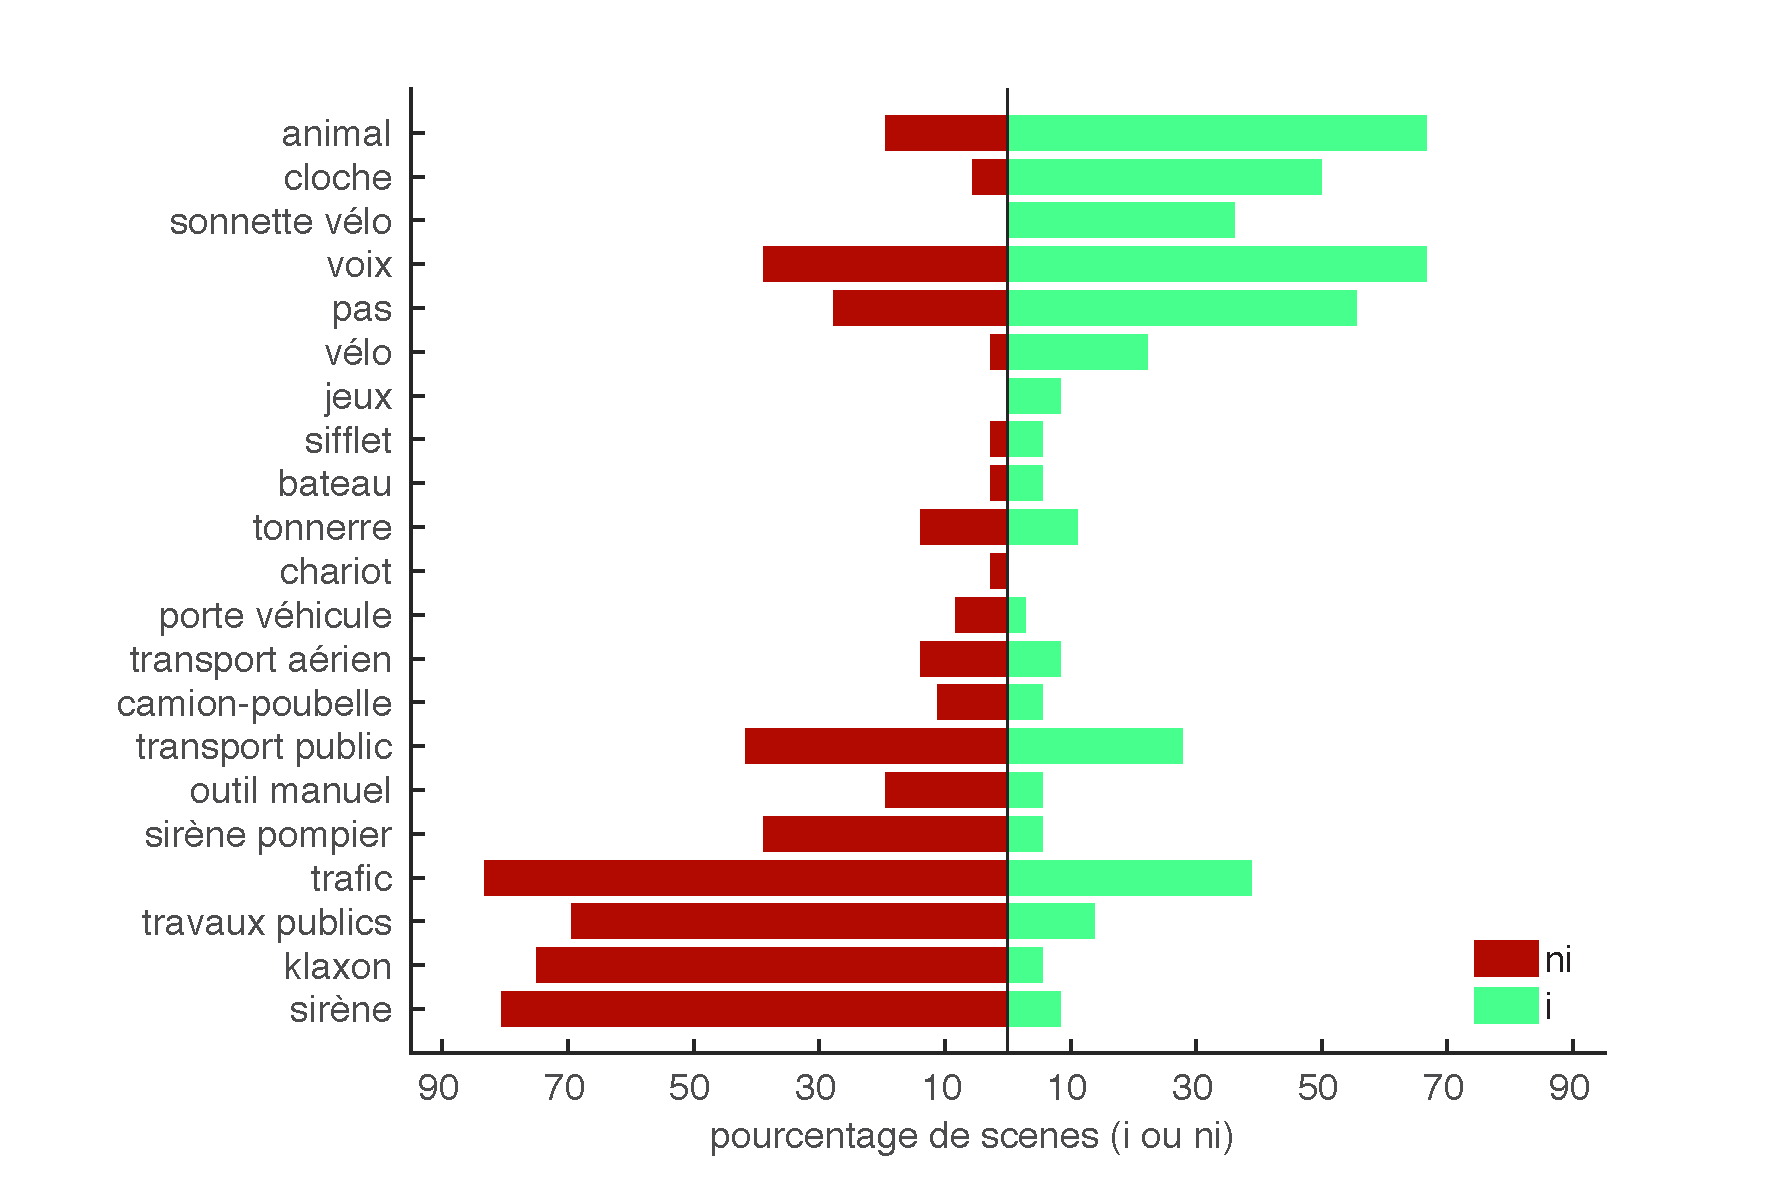
\includegraphics[width=1\linewidth]{gfx/ch_5/xp1_class_1_cam}\label{fig:soundsourcea}} \par
        \subfloat[]
        {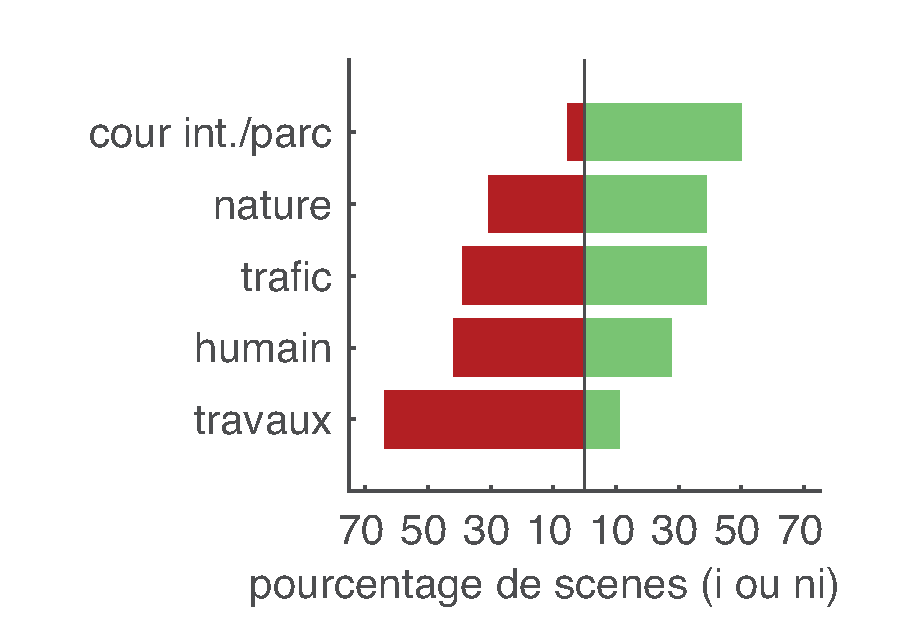
\includegraphics[width=.4\linewidth]{gfx/ch_5/xp1_class_2_cam}\label{fig:soundsourceb}} 
        \subfloat[]
        {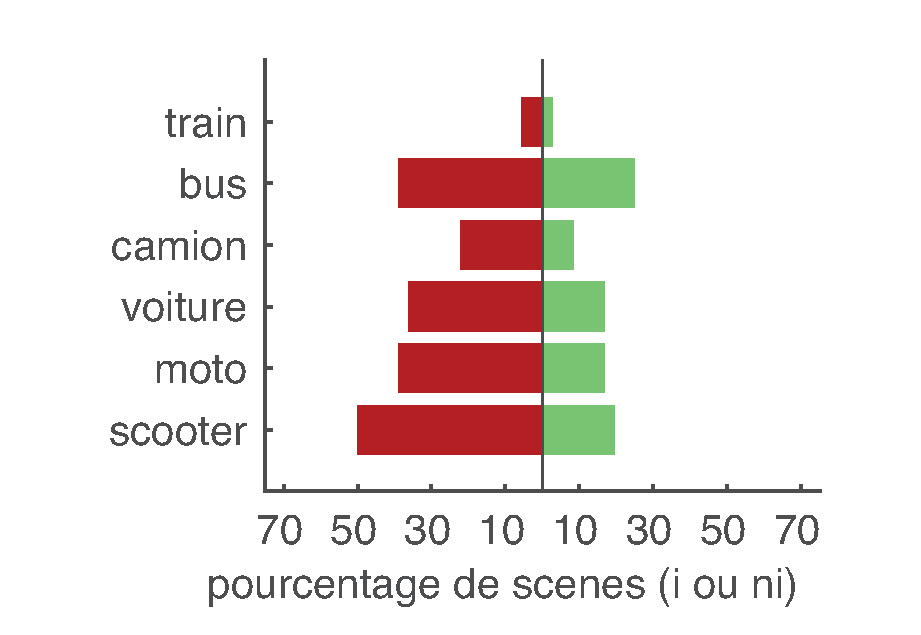
\includegraphics[width=.4\linewidth]{gfx/ch_5/xp1_class_3_cam}\label{fig:soundsourcec}} 
       \caption[Pourcentage de scènes simulées comportant une classe de son particulière.]{Pourcentage de scènes simulées (i ou ni) comportant une classe de son particulière: (a) classes d'événements du niveau d'abstraction $0+$, (b) classes de textures du niveau d'abstraction $0$, (c) sous classes d'événements du niveau d'abstraction 1 des classes \emph{trafic} et \emph{transport public} du niveau d'abstraction 0.}\label{fig:soundsource}
\end{figure}

\subsubsection{Marqueurs sonores}
\label{sec:ch5_marqueurXp1}

Nous avons mis en évidence que, qualitativement, la composition des sources sonores des scènes diffère selon les types d'environnement (i ou ni). Nous essayons de voir maintenant si, parmi ces classes, certaines sont typiques d'un environnement en particulier. Pour ce faire, nous utilisons le V-test (\cf~Section~\ref{sec:ch5_methodoEtStat1}), en considérant séparément chaque niveau d'abstraction. Les résultats sont présentés dans le tableau~\ref{tab:markers}.

Concernant les événements sonores, 9 marqueurs sont identifiés sur l'ensemble des niveaux d'abstraction. Comme la figure~\ref{fig:soundsource} le laissait présager, les classes relatives à l'activité humaine (\emph{pas homme béton}, \emph{sonnette vélo}), et à la nature (\emph{animaux, oiseaux}, \emph{chants d'oiseaux}) sont des marqueurs de i-scènes. Nous notons également la présence de la classe \emph{cloche} dans les marqueurs d'un environnement idéal. Ce fait est possiblement dû au \emph{background} socio-culturel des sujets, dans leur grande majorité, des citoyens européens. En effet, selon Schafer, un son reconnu par un individu comme faisant partie intégrante de son environnement est bien accepté. Les marqueurs de ni-scènes sont des classes faisant référence à des sons de travaux (\emph{travaux}), ou suggérant un trafic dense (\emph{klaxon}, \emph{sirène}).

Concernant les textures sonores, 5 marqueurs sont identifiés. Pour les i-scènes, il s'agit de classes faisant référence à des ambiances amorphes, calmes, (\emph{cour-intérieur/parc} et \emph{parc}). Pour les ni-scènes, il s'agit, comme pour les événements, de classes faisant référence à des bruits de travaux (\emph{travaux} et \emph{véhicule de travaux}), ainsi que d'une classe faisant référence au trafic (\emph{carrefour}).

Bien que l'ensemble des marqueurs identifiés soient intuitifs, aucune des classes d'événements faisant directement référence aux bruits de véhicules motorisés n'est un marqueur, exception faite de la classe de textures \emph{carrefour}. Pour représenter un trafic désagréable, les sujets ont porté leurs choix sur les classes \emph{klaxon} et \emph{sirène}. On peut supposer que les sons isolés de véhicules sont compris comme faisant partie intégrante de l'environnement urbain, et ne sont donc pas particulièrement associés à un environnement désagréable. \\ 

%\gl{TODO: ici analyse des caractéristiques des classes trafics} \\
%\gl{TODO: ici reprendre les conclusions de \citep{lavandier2006contribution} et \citep{ricciardi2015sound}}

\begin{table}[t]
 \setlength{\tabcolsep}{0.2pt}
 \centering
  {\renewcommand{\arraystretch}{0.9}
\begin{tabular}{c c c c} 
Niveau        & \multicolumn{2}{c}{Marqueurs sonores événements} \\
d'abstraction & i-scènes & ni-scènes \\
\hline
0  &                          &  travaux (3.78)  \\
\hline
  & cloche  (4.5)             & klaxon  (3.9) \\
1 & sonnette vélo  (4.3)      & sirène (3.9)\\
  & animal (4.2)              &       \\
   \hline
  & oiseau        (4.8)       & klaxon  (4.0)\\
2 & cloche  (4.4)             & sirène (4.0)\\
  & sonnette vélo    (4.2)             &       \\
   \hline
  & chant oiseau (4.8)        & klaxon  (4.1)\\
3 & cloche   (4.3)            & sirène (4.0)\\
  & sonnette vélo     (4.2)   &       \\
  & pas chaussure  (3.6)      &  \\
  &                           & \\ 
  & \multicolumn{2}{c}{Marqueurs sonores textures}      \\
  & i-scènes & ni-scènes \\
\hline
0 &     cour int./parc (4.1) &  travaux (3.9)  \\
\hline
1 &     parc (3.65)          &  carrefour (3.6)  \\
  &                          &  travaux véhicule (3.3)  \\
\hline
2 &     parc (3.64)          &  carrefour (3.56)  \\
\hline
\end{tabular}
} 
\vspace{0.5mm}
\caption[Classes d'événements et de textures identifiées comme étant des marqueurs sonores.]{Classes d'événements et de textures identifiées comme étant des marqueurs sonores. Dans chaque cellule, les marqueurs sont ordonnés par ordre décroissant de valeur $V$.}
\label{tab:markers}
\end{table}

\subsection{Étude des espaces de représentation induits par les descripteurs sémantiques}

Dans cette partie, nous évaluons la capacité d'une représentation sémantique à séparer les deux types d'environnements. Pour ce faire, nous calculons une précision au rang 5 ($p@5$) sur l'espace induit par les descripteurs sémantiques $S$, et ce pour chaque niveau d'abstraction (\cf~Section~\ref{sec:ch5_methodoEtStat1}). Les vecteurs $S$ sont construits en utilisant toutes les classes ($ET$), les classes d'événements ($E$), les classes de textures ($T$), les classes d'événements ne considérant que les marqueurs sonores ($E_m$), les classes d'événements ne considérant pas les marqueurs sonores $E_{w/o,m}$. Nous ne considérons pas les classes de marqueurs de textures, ces dernières étant trop peu nombreuses. Pour les mêmes raisons nous ne considérons pas les classes de marqueurs d'événements du niveau d'abstraction 0. Les résultats sont affichés sur la figure~\ref{fig:pa5}.

En ce qui concerne $ET$, la $p@5$ est de $76\%$ pour le niveau d'abstraction 0, et reste supérieure à $86\%$ à partir du niveau d'abstraction 1. Ces résultats confirment qu'il est possible de clairement distinguer les deux types d'environnements en se basant seulement sur la présence ou l'absence des classes de sons. Nous notons également que, plus le niveau d'abstraction est élevé, plus la capacité de séparer les environnements est importante. En d'autres termes, plus nous sommes précis dans notre description de la composition des scènes, plus nous sommes à même d'établir une distinction claire entre les i- et ni-scènes.

En considérant séparément $E$ et $T$, il apparaît que 1) la $p@5$ obtenue avec $E$ est similaire à celle obtenue avec $ET$, et 2) que la $p@5$ obtenue avec $T$ est systématiquement inférieure d'environ $10$ à $15\%$ à celle de $E$. Ces résultats indiquent que l'information sémantique permettant de séparer les deux environnements est principalement portée par les événements. Ces résultats font, par ailleurs, écho aux travaux de  \citep{maffiolo_caracterisation_1999}, qui montrent que nous analysons de manière descriptive (en identifiant les sources) les scènes événementielles, \ie~composées d'événements sonores (\cf~Section~\ref{sec:ch3_catsoundscape}).

Enfin, il apparaît que la $p@5$ obtenue avec $E_{m}$ est égale, voire supérieure à celles de $E$ et $ET$, et ce bien qu'une information partielle soit utilisée dans ce cas pour décrire les scènes. La dimension des vecteurs de description $S$ pour $E_m$ est en effet inférieure à la dimension des vecteurs $S$ pour $E$, qui est elle même inférieure à celle obtenue dans le cas où toutes les classes sont utilisées ($ET$). De plus, dans le cas où les marqueurs ne sont pas pris en compte pour la description ($E_{w/o,m}$), les résultats chutent, passant même en dessous de ceux obtenus en ne considérant que les textures. Cela confirme que la majorité de l'information sémantique permettant de faire la distinction entre i-scènes et ni-scènes est incluse dans les marqueurs.

En résumé, nous déduisons de cette analyse les points suivants:

\begin{enumerate}
\item contrairement à ce que nous avions constaté avec les descripteurs structurels, une description sémantique de la composition des scènes, en terme de présence/absence de sources sonores, permet de bien distinguer les deux types d'environnements (i ou ni);
\item l'information sémantique est majoritairement portée par les classes d'événements sonores;
\item parmi les classes d'événements, seule une partie, \ie~les marqueurs sonores, est nécessaire pour faire la distinction entre les i- et ni-scènes.
\end{enumerate}

Maintenant que nous avons isolé les classes typiques des i- et ni-scènes, et vérifié que la distinction entre ces environnements dépendait de la présence de ces classes, il reste à voir si une description structurelle des scènes, basée uniquement sur ces marqueurs sonores, permet de caractériser l'agrément perçu, mieux qu'une description structurelle globale. 

\begin{figure}[t]
        \myfloatalign
        \includegraphics[width=.8\linewidth]{gfx/ch_5/pa5_1}
       \caption[$P@5$ obtenues en considérant la matrice de dissimilarité résultant des distances par paires de Hamming calculées entre les vecteurs des descripteurs sémantiques des scènes.]{$P@5$ obtenues en considérant la matrice de dissimilarité résultant des distances par paires de Hamming calculées entre les vecteurs des descripteurs sémantiques des scènes. Les vecteurs sont construits en utilisant toutes les classes ($ET$), les classes d'événements ($E$), les classes de textures ($T$), les classes d'événements ne considérant que les marqueurs sonores ($E_m$), les classes d'événements ne considérant pas les marqueurs sonores $E_{w/o,m}$.}\label{fig:pa5}
\end{figure}

\subsection{L'influence spécifique des marqueurs sonores sur l'agrément perçu}

\begin{table}[t]
\centering
\begin{tabular}{l r r} 
                  &   i-scenes                  & ni-scenes \\
\hline
$L_m$              & 0.03  ($p=0.88$)           & \textbf{-0.75} ($p<0.01$) \\
$L(E)_m$           & 0.08  ($p=0.66$)           & \textbf{-0.71} ($p<0.01$) \\
$L(T)_m$           & -0.11 ($p=0.66$)           & -0.17 ($p=0.37$) \\
$L_b$              & \textbf{-0.52} ($p<0.01$)  & -0.32 ($p=0.06$) \\
$L(E)_b$           & \textbf{-0.51} ($p<0.01$)  & -0.30 ($p=0.07$) \\
$L(T)_b$           & -0.32 ($p=0.05$)           & \textbf{-0.73} ($p<0.01$) \\
$L_m-L_b$          & \textbf{0.67} ($p<0.01$)   & -0.31 ($p=0.07$) \\
$L(E)_m-L(E)_b$    & \textbf{0.66} ($p<0.01$)   & -0.28 ($p=0.10$) \\
$L(T)_m-L(T)_b$    & 0.16 ($p=0.54$)            & 0.21 ($p=0.28$) \\
$D_m$              & 0.03 ($p=0.87$)            & -0.31 ($p=0.07$) \\
$D(E)_m$           & 0.14 ($p=0.41$)            & \textbf{-0.44} ($p<0.01$) \\
\hline
\end{tabular}
\vspace{0.5mm}
\caption{Coefficients de corrélation linéaire calculés entre l'agrément perçu moyen $\mathcal{A}_{scene}$ de l'expérience 1.b et les descripteurs structurels relatifs à la présence des marqueurs sonores.}
\label{tab:corrMarkers}
\end{table}

Comme pour la  section~\ref{sec:ch5_corrDesStruct}, nous évaluons les corrélations entre $\mathcal{A}_{scene}$ et les descripteurs structurels. Pour cette section, les descripteurs structurels sont calculés en tenant compte des marqueurs sonores précédemment identifiés. Nous définissons $X_m$ le descripteur $X$ calculé en ne prenant en compte que les sons des marqueurs. A l'inverse, nous définissons $X_b$ ($b$: pour « bruit ») le descripteur $X$ calculé en prenant en compte toutes les classes de sons excepté les marqueurs. Lorsque le descripteur caractérise une i-scène (idem pour une ni-scène), nous ne considérons, pour le calcul, que les marqueurs identifiés pour les i-scènes (ou pour les ni-scènes), que nous nommons i-marqueurs (ou ni-marqueurs). Les résultats sont affichés sur le tableau~\ref{tab:corrMarkers}.

Considérons dans un premier temps les densités (\cf~Figures~\ref{fig:densityMarker}). Les résultats pour $D_m$ et $D(E)_m$ sont similaires à ceux observés précédemment pour $D$ et $D(E)$, a l'exception de $D_m$ qui ne présente plus une corrélation significative pour les ni-scènes. Ces résultats tendent à confirmer que la densité est un indicateur d'agrément de faible importance, qu'on la considère globalement, ou en prenant en compte les contributions séparées de différentes sources. \\

%\gl{TODO: Rajouter $D_b$ + comparaison par pair des descripteurs de marqueurs} \\

Concernant les niveaux sonores (\cf~Figures~\ref{fig:soundlevelMarker}), là encore les mêmes tendances sont observées entre $L_m$, $L(E)_m$ et $L(T)_m$, d'une part, et $L$, $L(E)$ et $L(T)$, d'autre part. Que l'on considère uniquement les marqueurs, ou l'ensemble des classes, il s'avère que :

\begin{enumerate}
\item il existe une différence significative entre les niveaux des i- et ni-scènes ($L_m$, $L(E)_m$ et $L(T)_m$: $p<0.01$);
\item le niveau sonore des scènes est majoritairement porté par les événements sonores, comparé aux textures sonores;
\item le niveau sonore des événements a une influence sur la perception de l'agrément pour les ni-scènes, mais pas pour les i-scènes;
\item le niveau sonore des textures ne joue aucun rôle dans la perception de l'agrément.
\end{enumerate}

En conclusion, le niveau des ni-marqueurs a une influence négative sur l'agrément pour les ni-scènes. En revanche le niveau des i-marqueurs n’impacte pas l'agrément perçu pour les i-scènes.

En considérant maintenant les classes non marqueurs  (\cf~Figures~\ref{fig:soundlevelNoise}), nous remarquons, sur les i-scènes, une corrélation négative modérée/faible pour $L_b$  ($r=-52$, $p<0.01$) et $L(E)_b$ ($r=-51$, $p<0.01$). C'est la première fois qu'un indicateur objectif nous permet de préciser l'agrément des environnements agréables. Ceci nous amène à conclure que le niveau des classes de sons n'étant pas typiques d'un environnement agréable a un impact négatif sur l'agrément. 

Par ailleurs, alors que $L(T)$ ne présentait pas de corrélation pour les ni-scènes, une corrélation négative forte est observée pour $L(T)_b$ ($r-0.73$, $p<0.01$). Ce fait indique que les niveaux des classes de textures n'étant pas des marqueurs n'affectent pas l'agrément perçu de la même manière pour les i- et ni-scènes. Les niveaux semblent avoir un effet négatif pour les ni-scènes, alors que pour les i-scènes, aucun effet n'est relevé.

Pour finir, nous considérons un dernier groupe de descripteurs, nommément $L_m-L_b$, $L(E)_m-L(E)_b$ et $L(T)_m-L(T)_b$ (\cf~Figures~\ref{fig:soundlevelMarkerDiff}). Ces descripteurs expriment la différence entre les niveaux des marqueurs, et ceux des autres classes de sons. Ils traduisent l'émergence des marqueurs par rapport à la mixture sonore.

Pour les i-scènes, une corrélation modérée et positive est observée pour $L_m-L_b$ ($r=0.67$, $p<0.01$) et $L(E)_m-L(E)_b$ ($r=0.66$, $p<0.01$). Pour les ni-scènes, aucune corrélation n'est observée. Dans le cas des i-scènes, ce n'est donc pas le niveau absolu des marqueurs qui importe, mais leur niveau relatif, par rapport aux autres sons qui composent la scène. On observe donc pour les environnements idéaux un double mécanisme perceptif: 

\begin{itemize}
\item plus le niveau absolu des sons n'étant pas des i-marqueurs est élevé, plus l'agrément est faible,
\item plus le niveau relatif des i-marqueurs, par rapport aux autres sons, est élevé, plus l'agrément est élevé.
\end{itemize}

Pour les ni-scènes, le fait que nous observions des corrélations pour $L_m$ et $L(E)_m$, et aucune pour $L_m-L_b$ et $L(E)_m-L(E)_b$, montre que c'est bien le niveau absolu qui importe.

\begin{figure}[t]
        \myfloatalign
        \subfloat[]
        {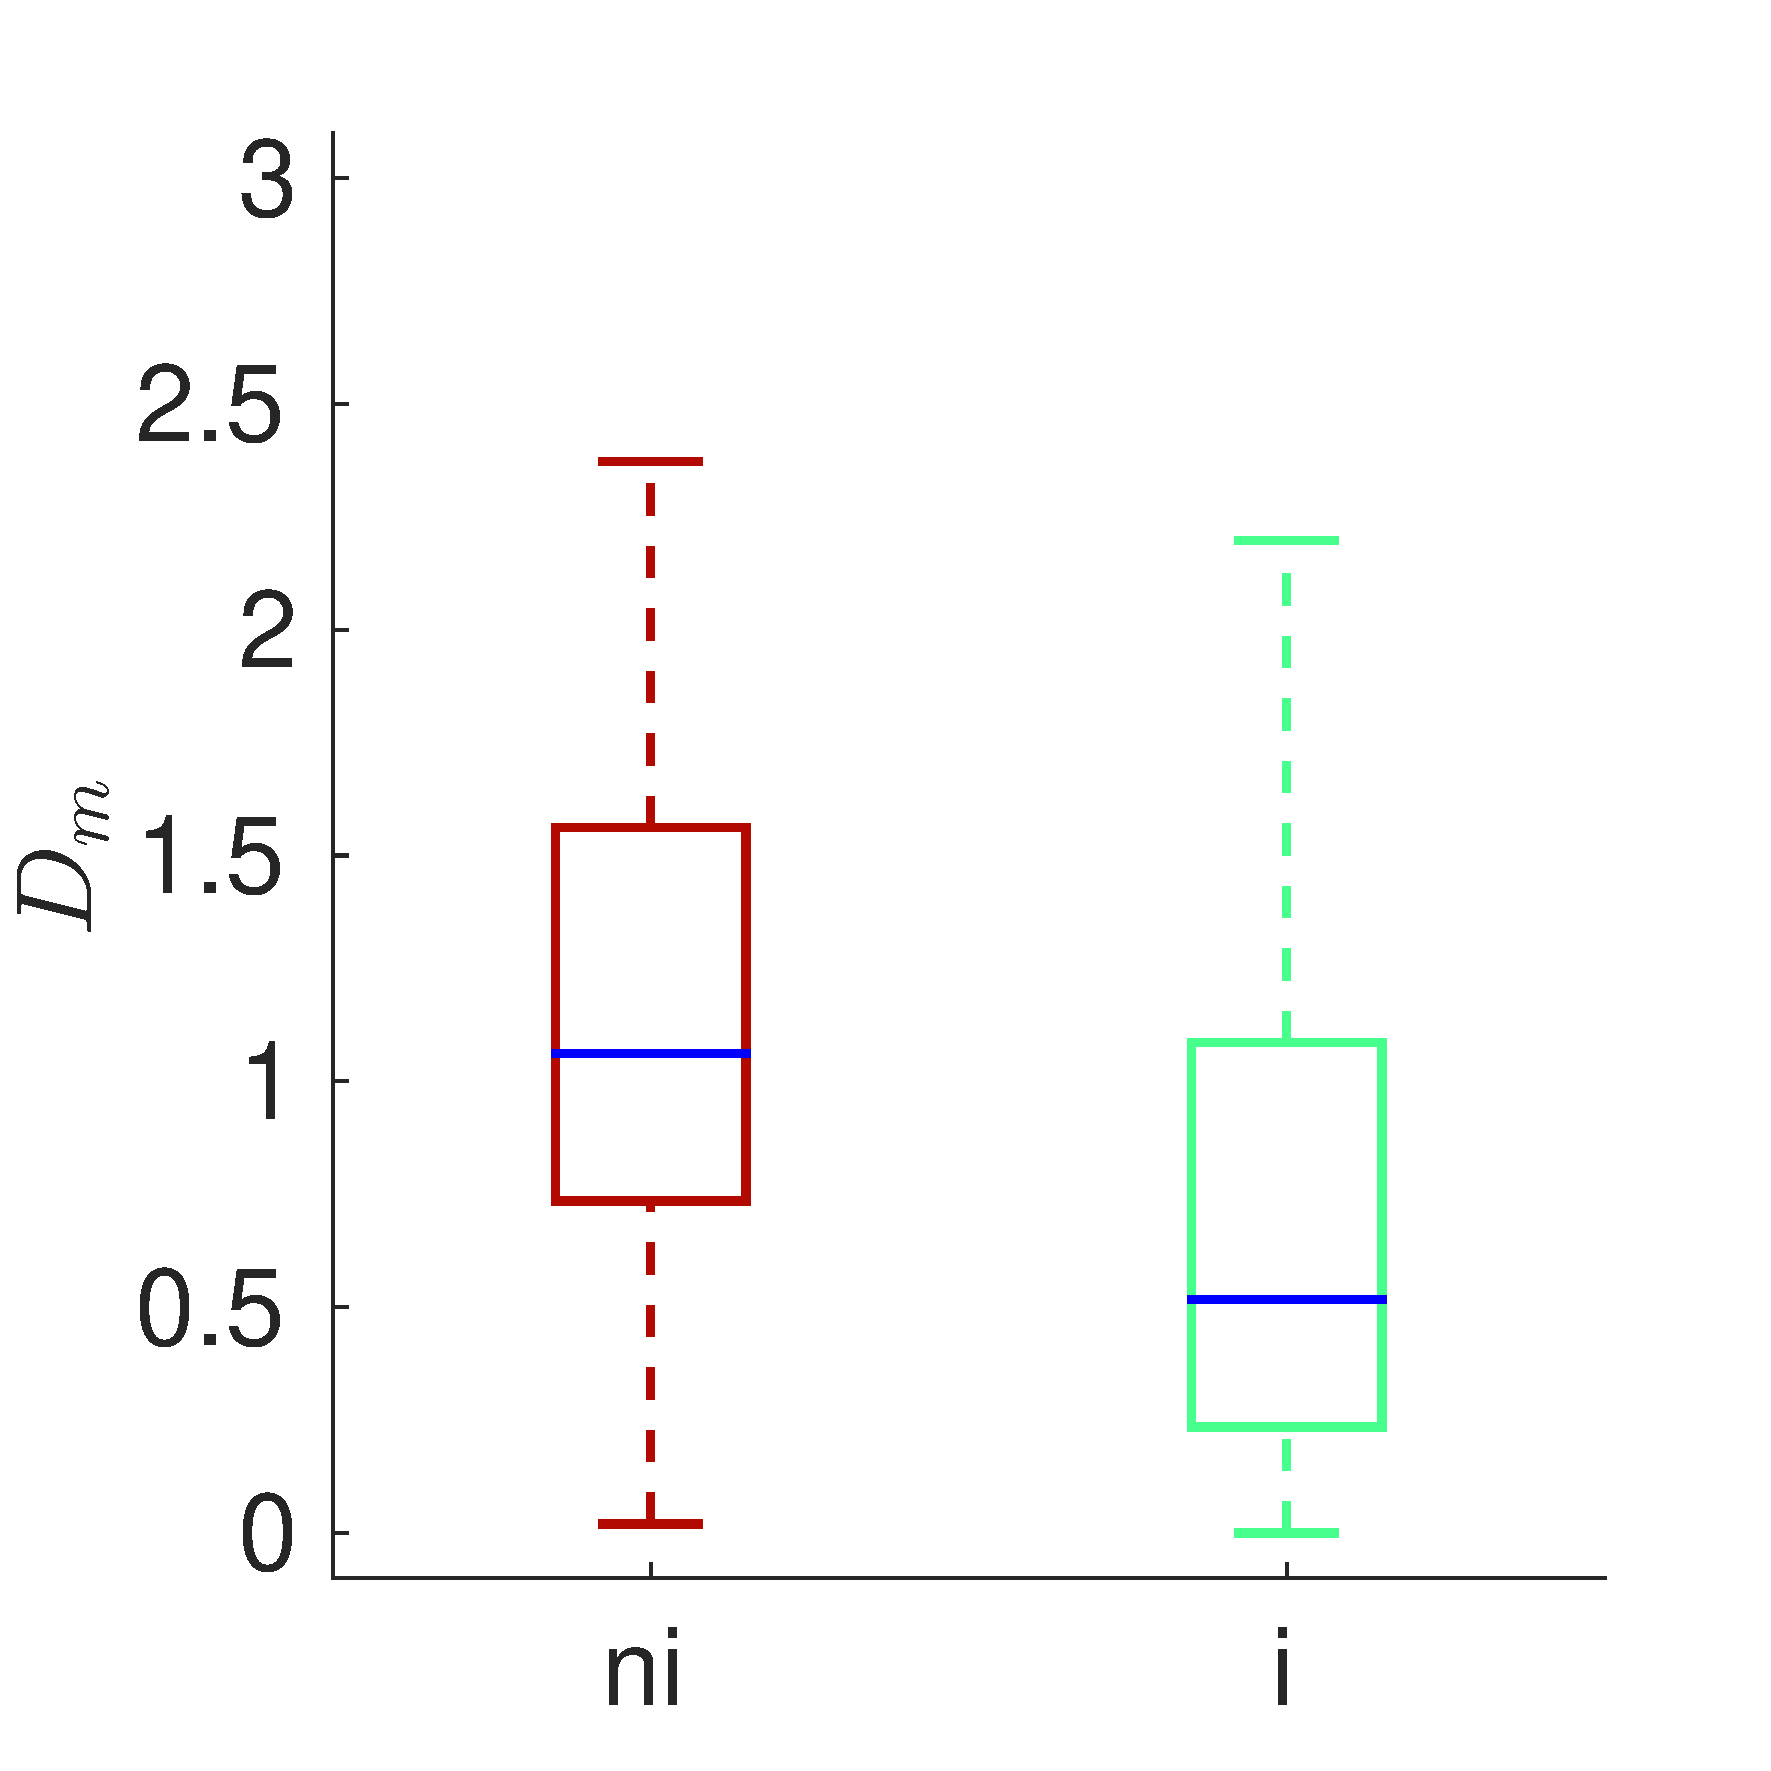
\includegraphics[width=.33\linewidth]{gfx/ch_5/xp_density_7}\label{fig:densityMarkera}}
        \subfloat[]
        {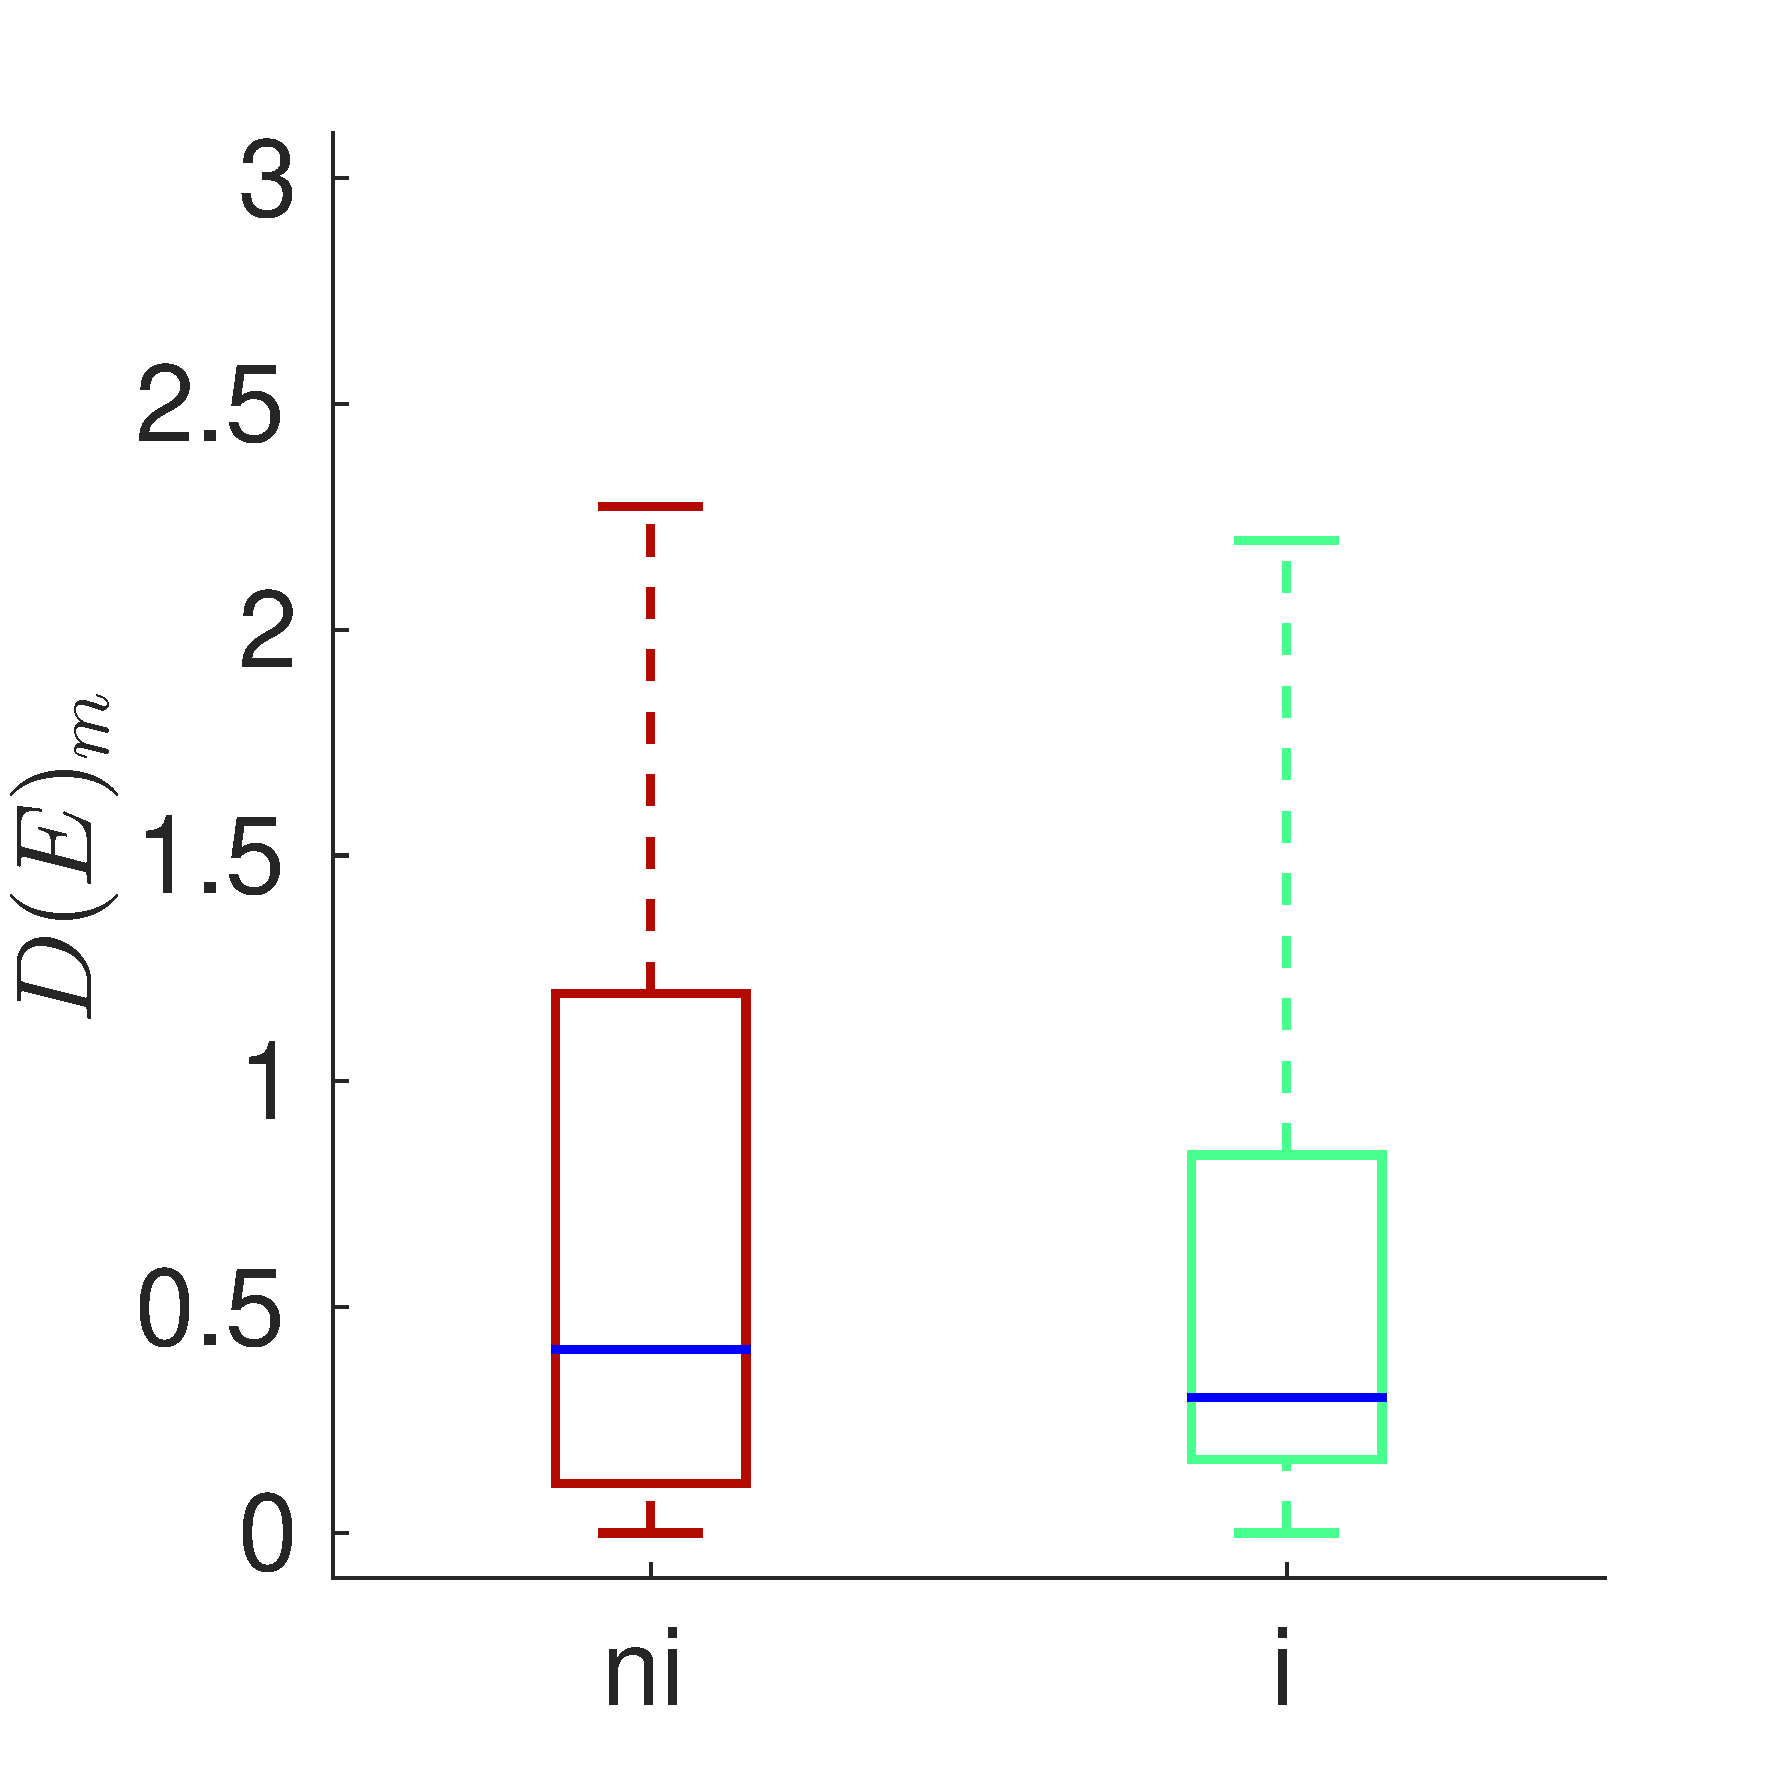
\includegraphics[width=.33\linewidth]{gfx/ch_5/xp_density_9}\label{fig:densityMarkerb}}\par
        \subfloat[]
        {\includegraphics[width=.33\linewidth]{gfx/ch_5/xp_density_8}\label{fig:densityMarkerc}}
        \subfloat[]
        {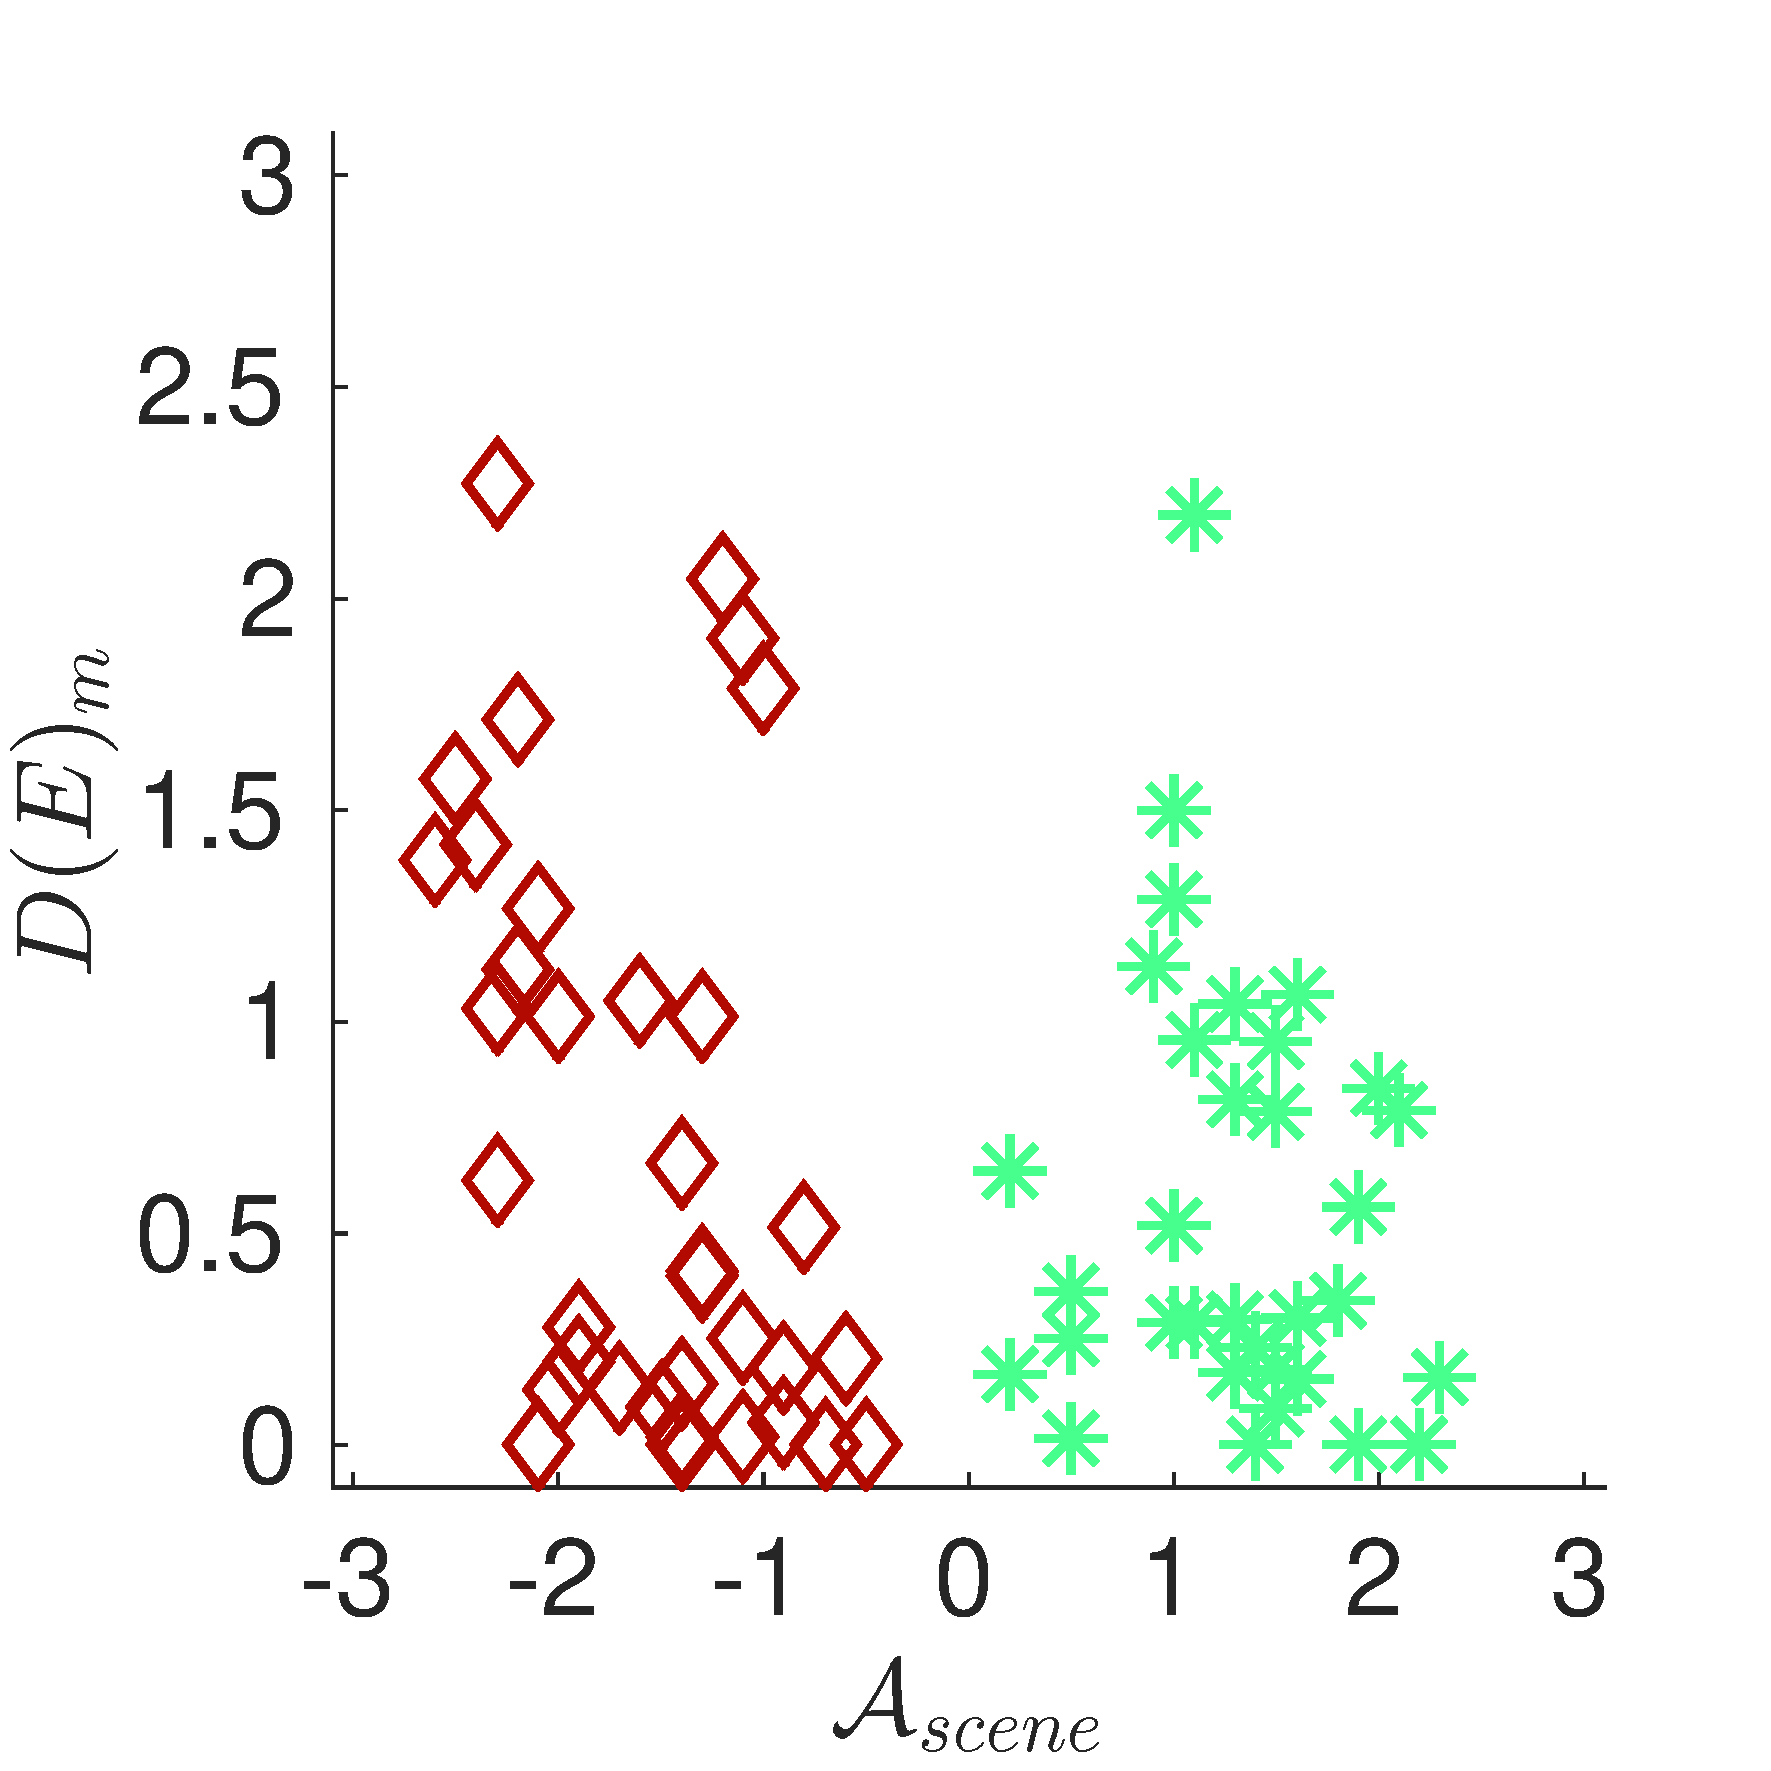
\includegraphics[width=.33\linewidth]{gfx/ch_5/xp_density_10}\label{fig:densityMarkerd}}
       \caption{Dispersions des descripteurs structurels de densité relatif à la présence des marqueurs $D_m$ (a, c) et $D(E)_m$ (b, d), en fonction du type de scènes (a, b) et de l'agrément perçu $\mathcal{A}_{scene}$ de l'expérience 1.b (c, d).}\label{fig:densityMarker}
\end{figure}

\begin{figure}[t]
        \myfloatalign
        \subfloat[]
        {\includegraphics[width=.33\linewidth]{gfx/ch_5/xp_soundlevel_7}\label{fig:soundlevelMarkera}}
        \subfloat[]
        {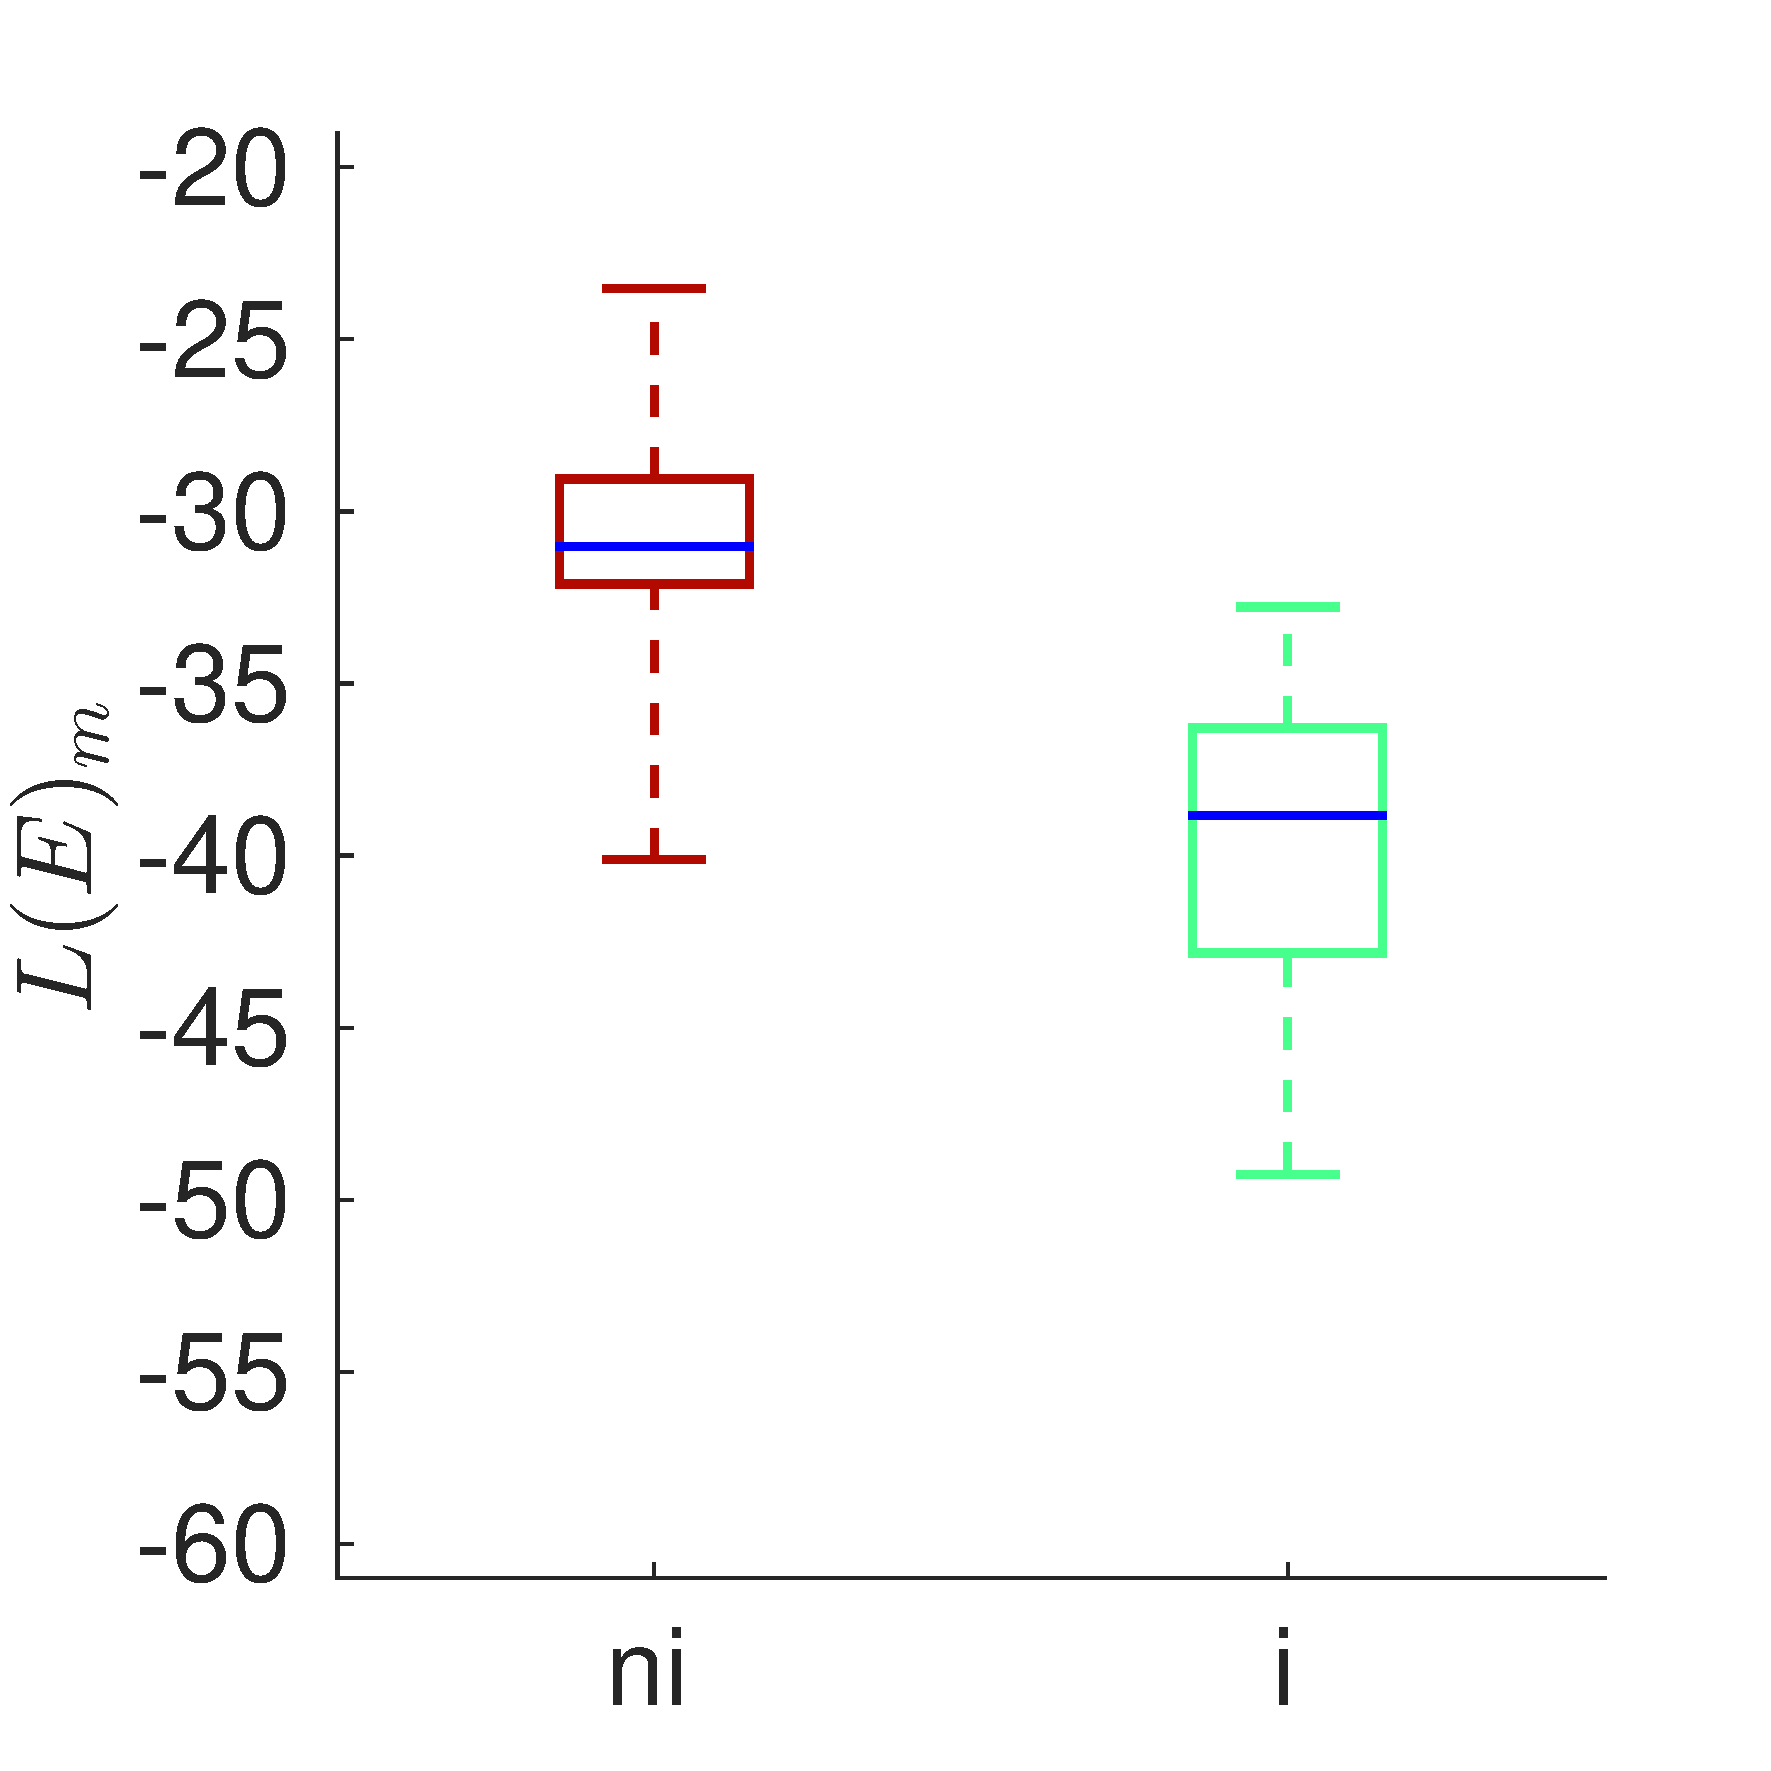
\includegraphics[width=.33\linewidth]{gfx/ch_5/xp_soundlevel_11}\label{fig:soundlevelMarkerb}}
        \subfloat[]
        {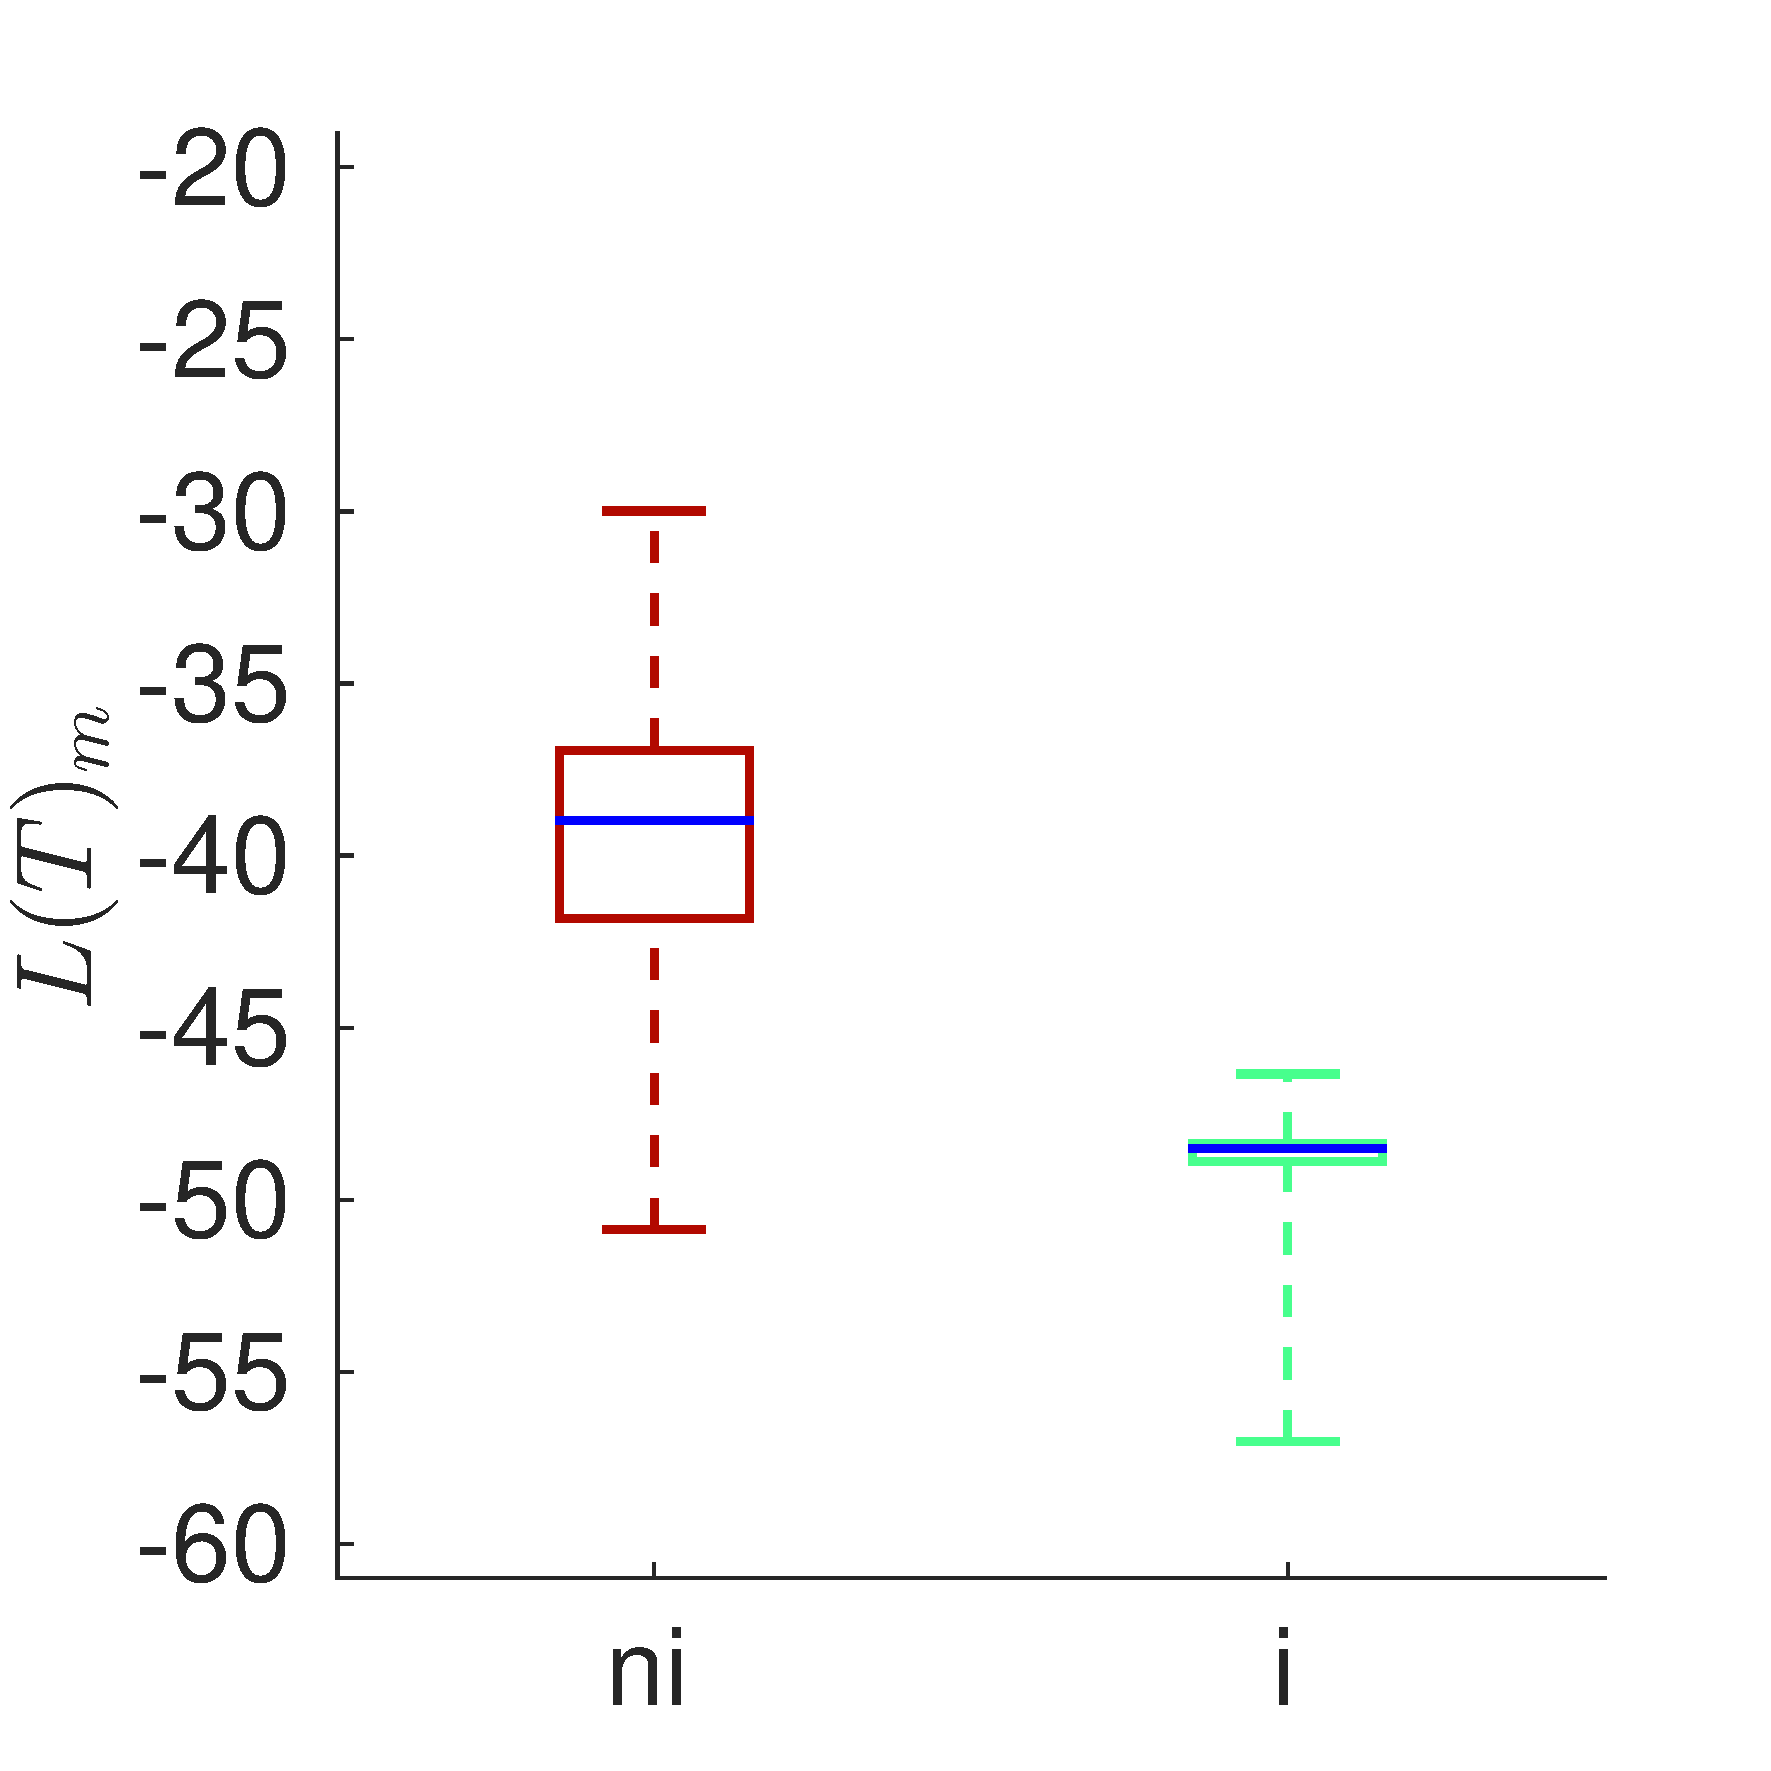
\includegraphics[width=.33\linewidth]{gfx/ch_5/xp_soundlevel_15}\label{fig:soundlevelMarkerc}}\par
        \subfloat[]
        {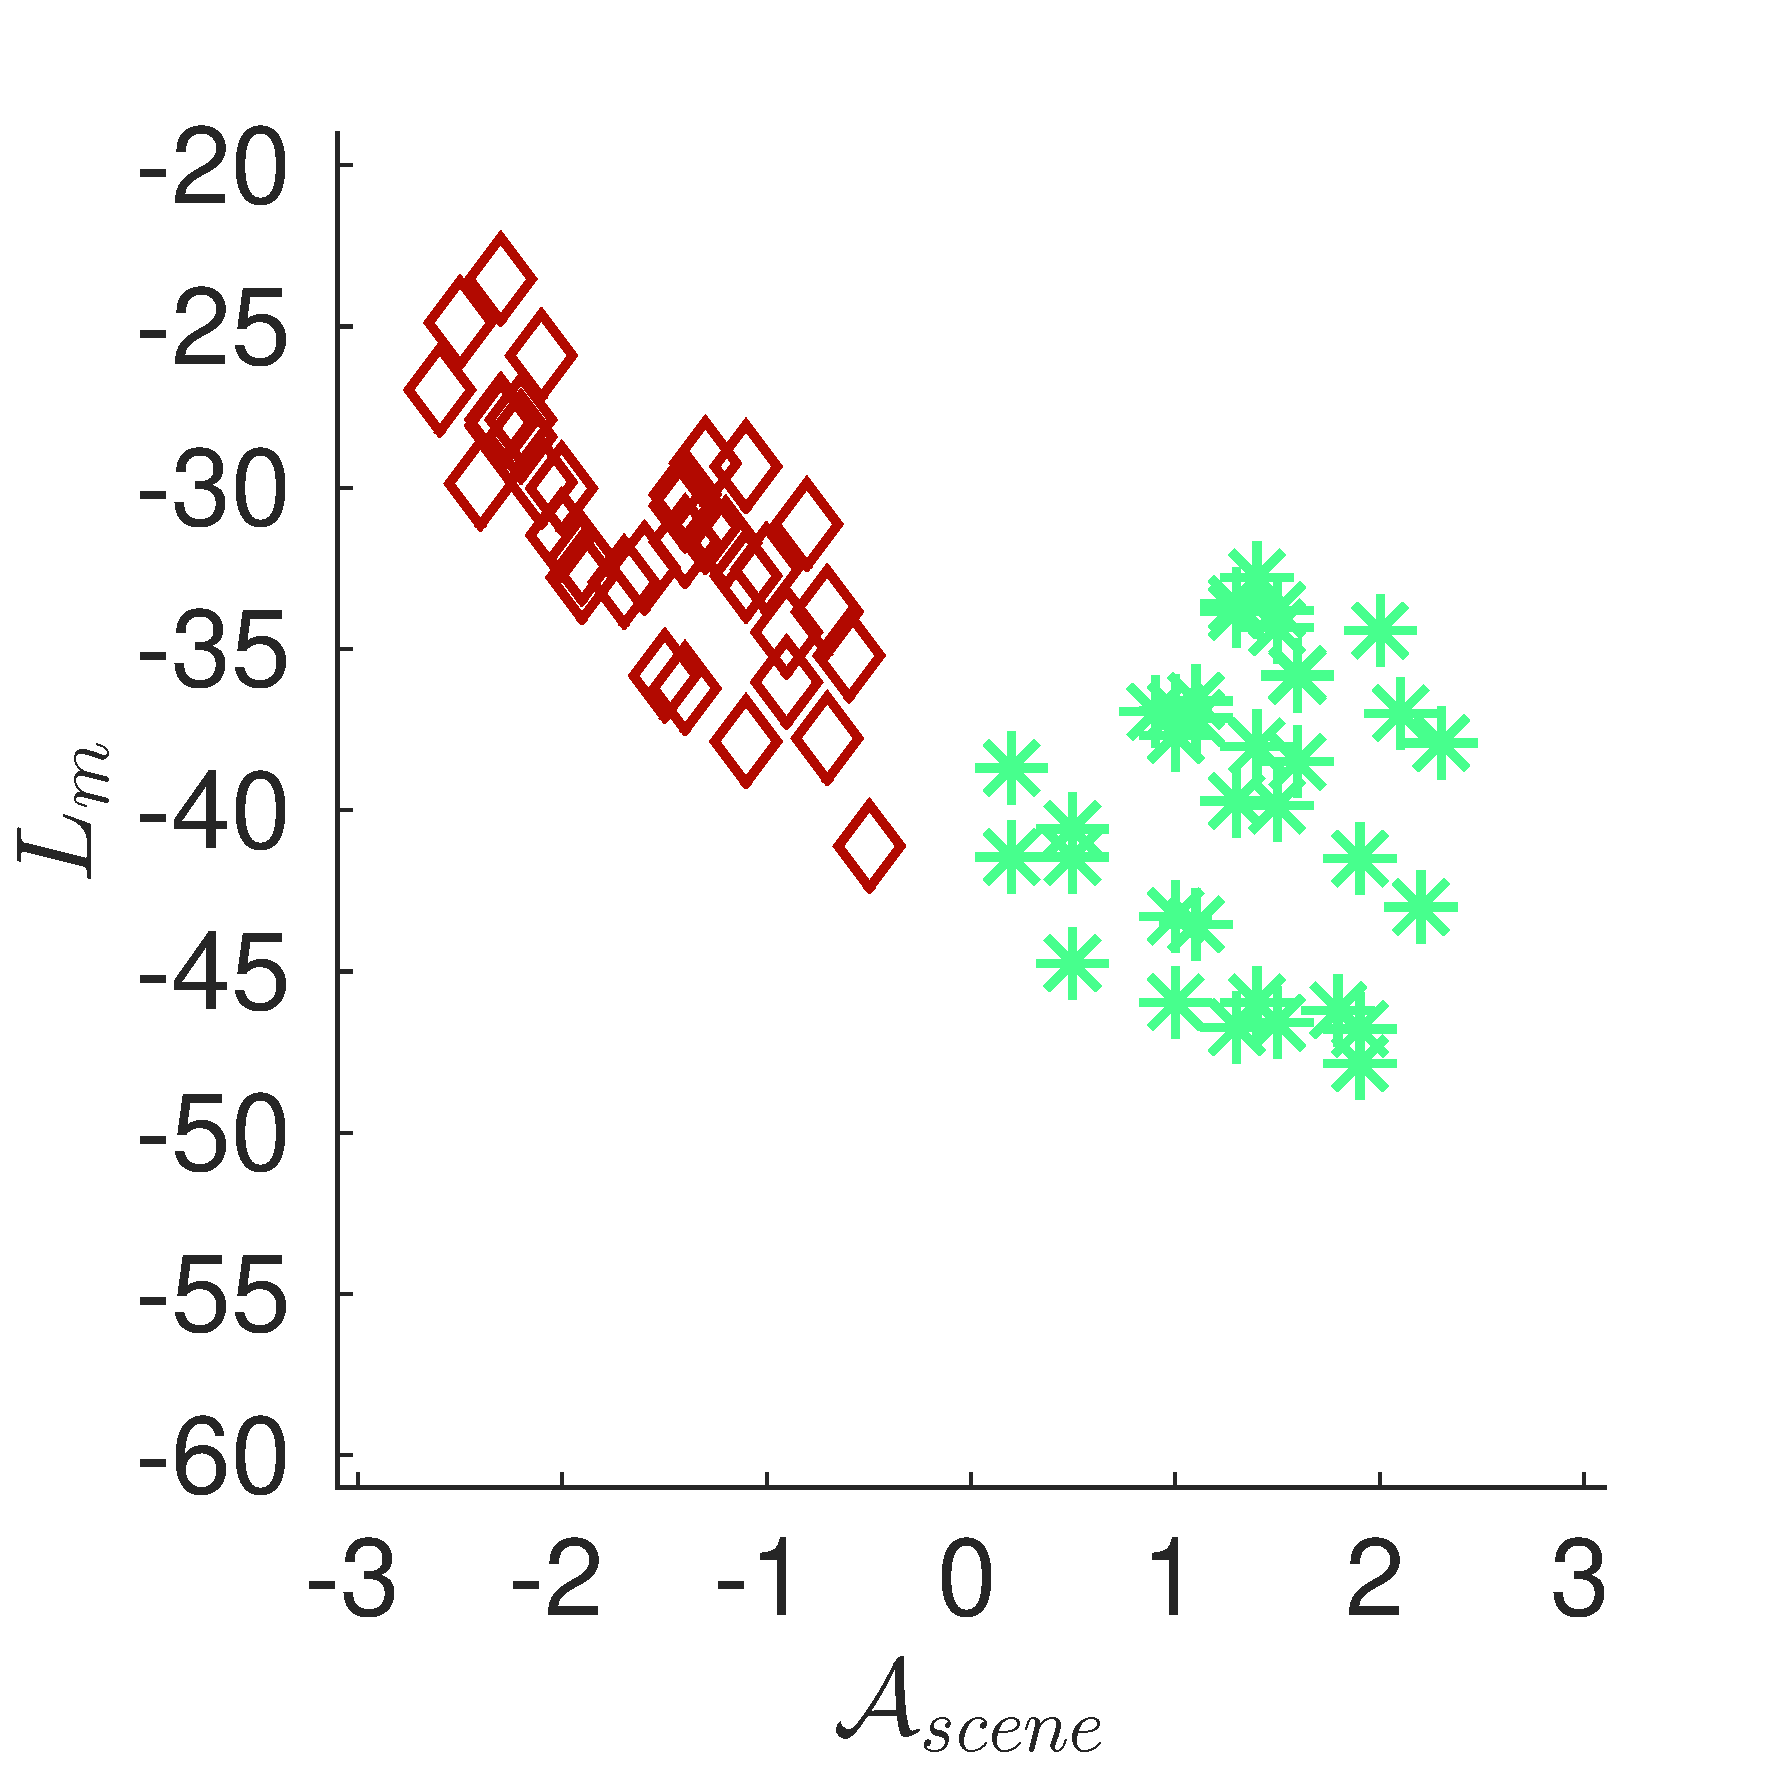
\includegraphics[width=.33\linewidth]{gfx/ch_5/xp_soundlevel_8}\label{fig:soundlevelMarkerd}}
        \subfloat[]
        {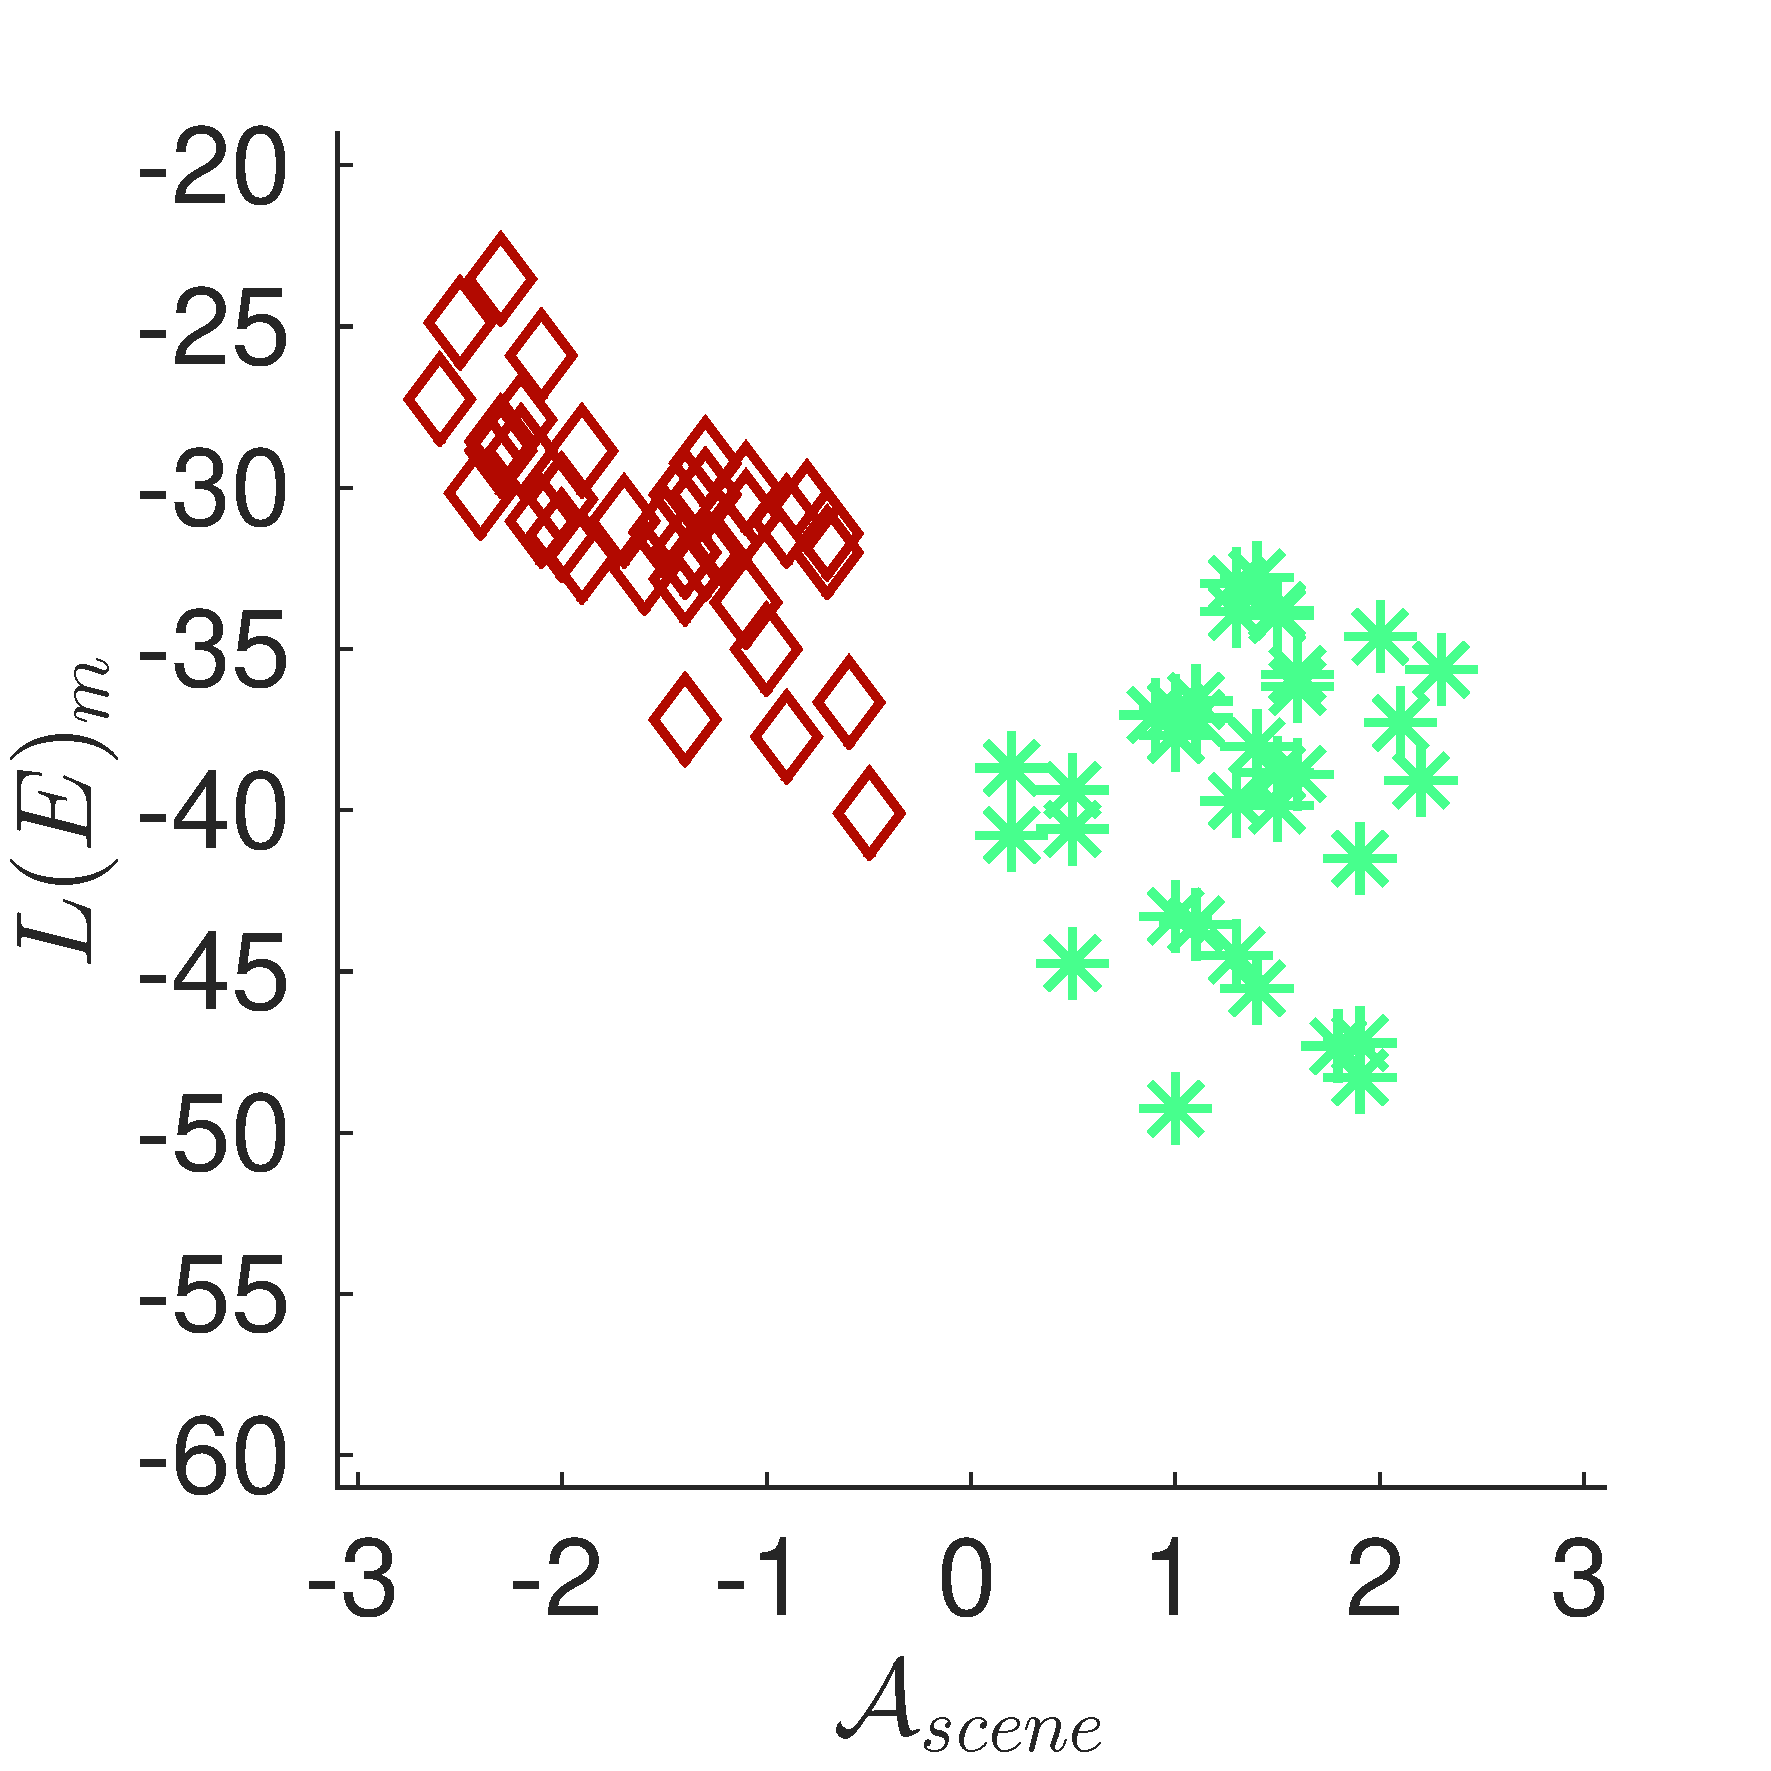
\includegraphics[width=.33\linewidth]{gfx/ch_5/xp_soundlevel_12}\label{fig:soundlevelMarkere}}
        \subfloat[]
        {\includegraphics[width=.33\linewidth]{gfx/ch_5/xp_soundlevel_16}\label{fig:soundlevelMarkerf}}       
        \caption{Dispersions des descripteurs structurels de niveaux sonores relatifs à la présence des marqueurs $L_m$ (a, d), $L(E)_m$ (b, e) et $L(T)_m$ (c, f), en fonction du type de scènes (a, b, c) et de l'agrément perçu $\mathcal{A}_{scene}$ de l'expérience 1.b (d, e, f).}\label{fig:soundlevelMarker}
\end{figure}

\begin{figure}[t]
        \myfloatalign 
        \subfloat[]
        {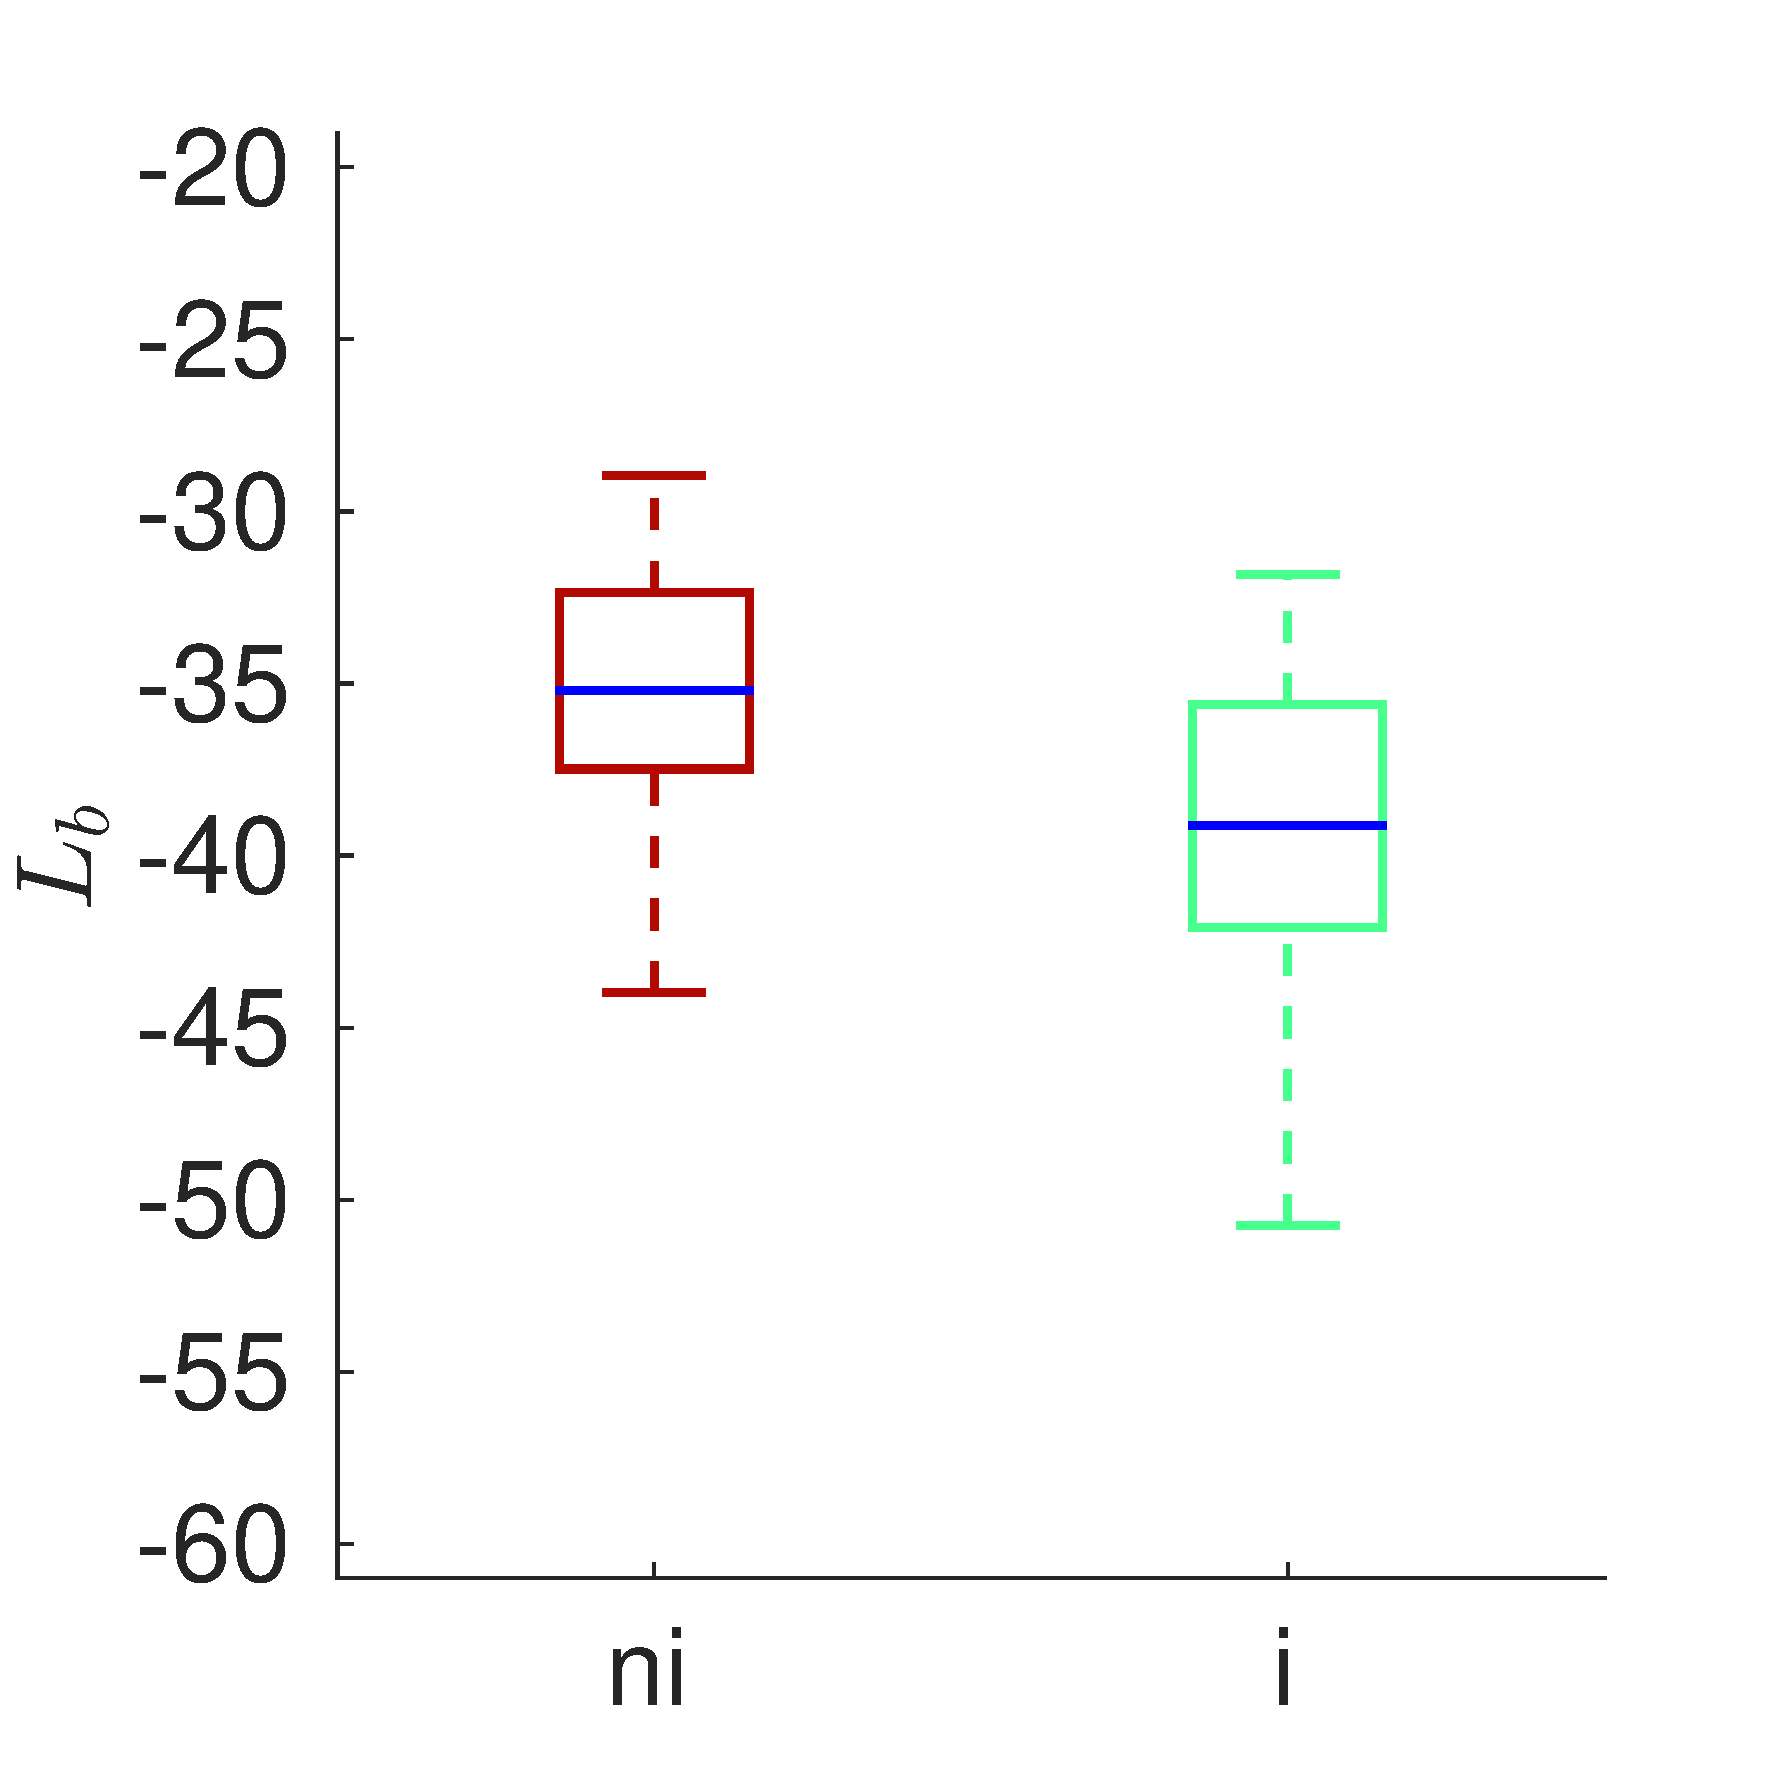
\includegraphics[width=.33\linewidth]{gfx/ch_5/xp_soundlevel_9}\label{fig:soundlevelNoisea}}
        \subfloat[]
        {\includegraphics[width=.33\linewidth]{gfx/ch_5/xp_soundlevel_13}\label{fig:soundlevelNoiseb}}
        \subfloat[]
        {\includegraphics[width=.33\linewidth]{gfx/ch_5/xp_soundlevel_17}\label{fig:soundlevelNoisec}}\par
        \subfloat[]
        {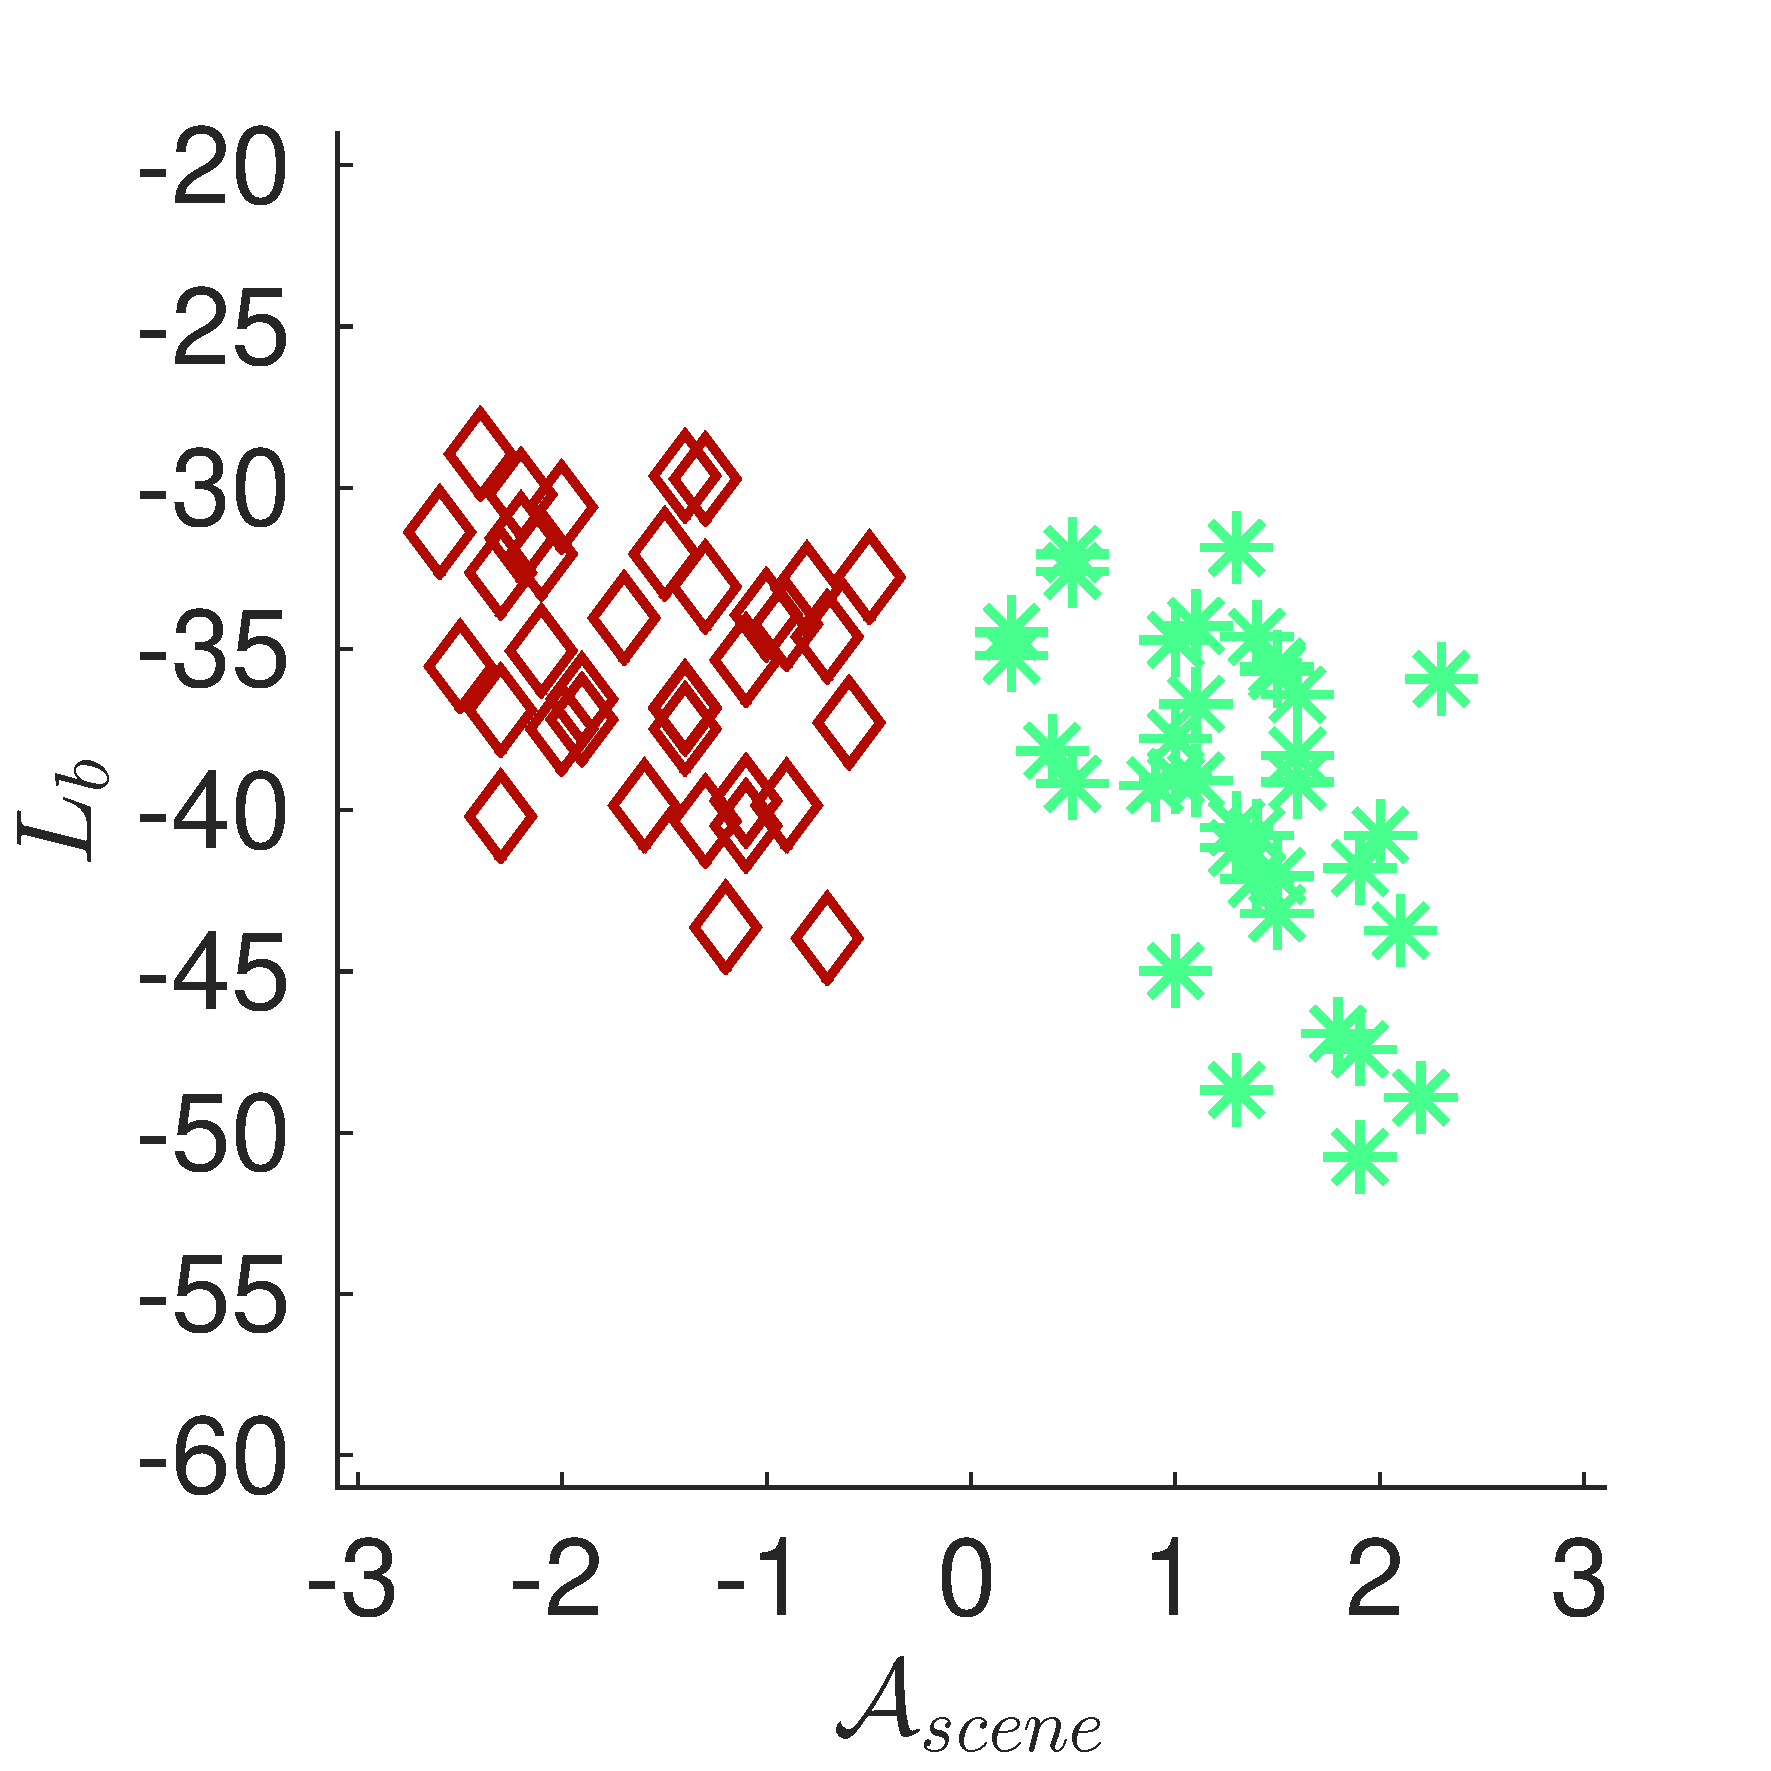
\includegraphics[width=.33\linewidth]{gfx/ch_5/xp_soundlevel_10}\label{fig:soundlevelNoised}}
        \subfloat[]
        {\includegraphics[width=.33\linewidth]{gfx/ch_5/xp_soundlevel_14}\label{fig:soundlevelNoisee}}
        \subfloat[]
        {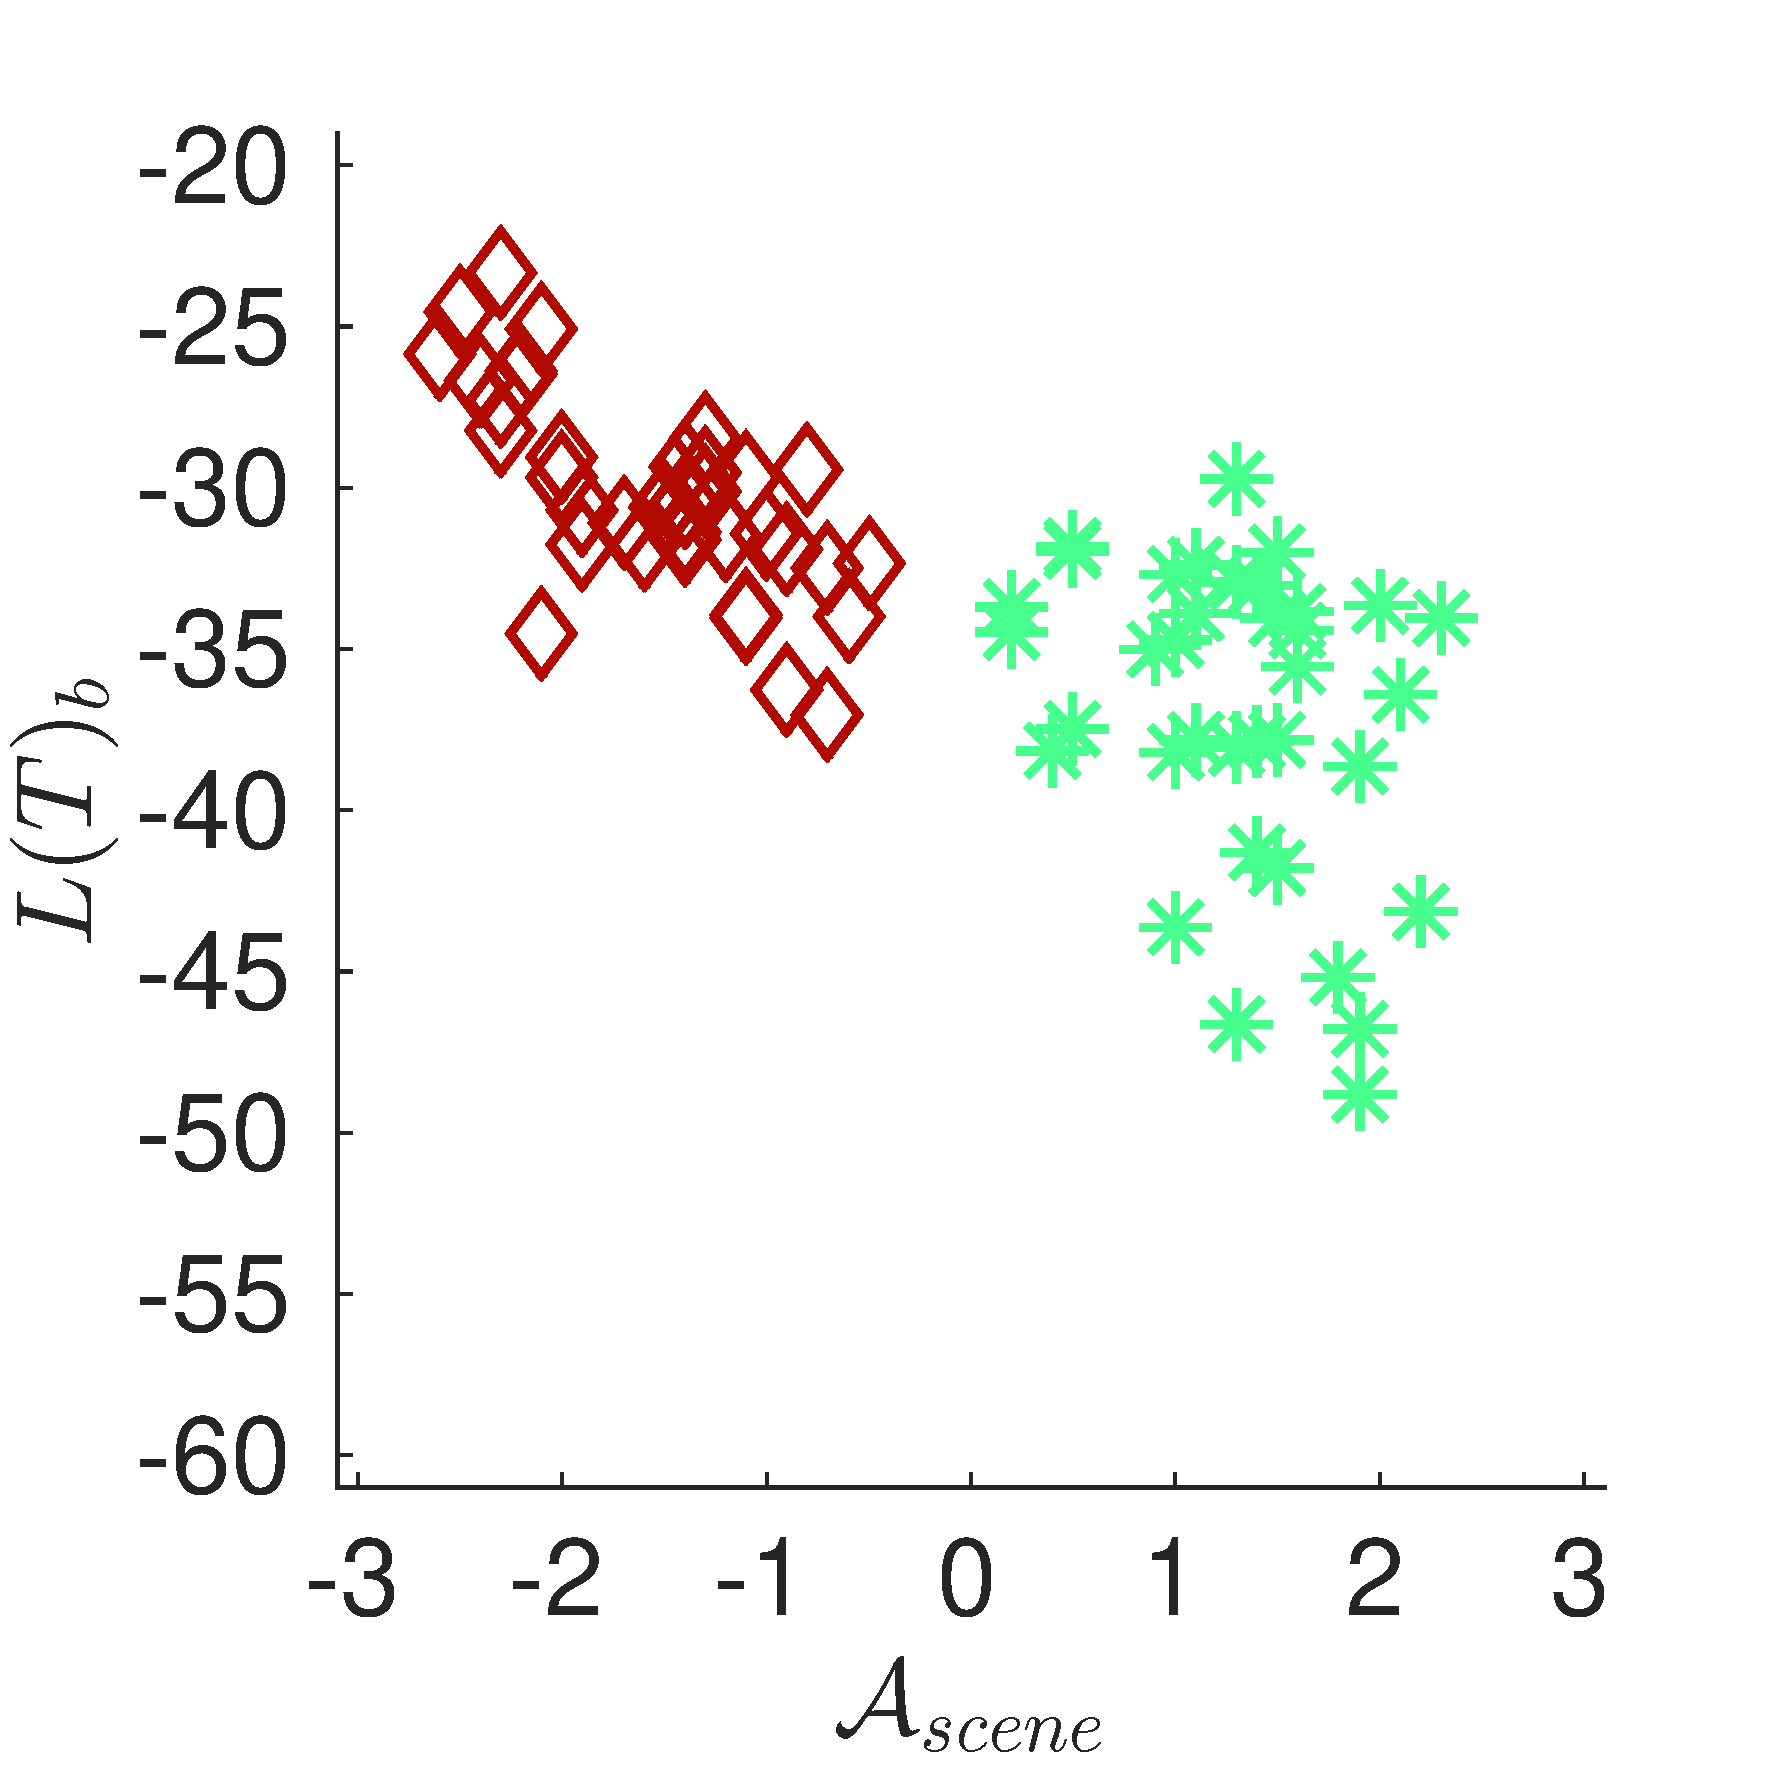
\includegraphics[width=.33\linewidth]{gfx/ch_5/xp_soundlevel_18}\label{fig:soundlevelNoisef}}
       \caption{Dispersions des descripteurs structurels de niveaux sonores relatifs à la présence des marqueurs $L_b$ (a, d), $L(E)_b$ (b, e) et $L(T)_b$ (c, f), en fonction du type de scènes (a, b, c) et de l'agrément perçu $\mathcal{A}_{scene}$ de l'expérience 1.b (d, e, f).}\label{fig:soundlevelNoise}
\end{figure}

\begin{figure}[t]
        \myfloatalign 
        \subfloat[]
        {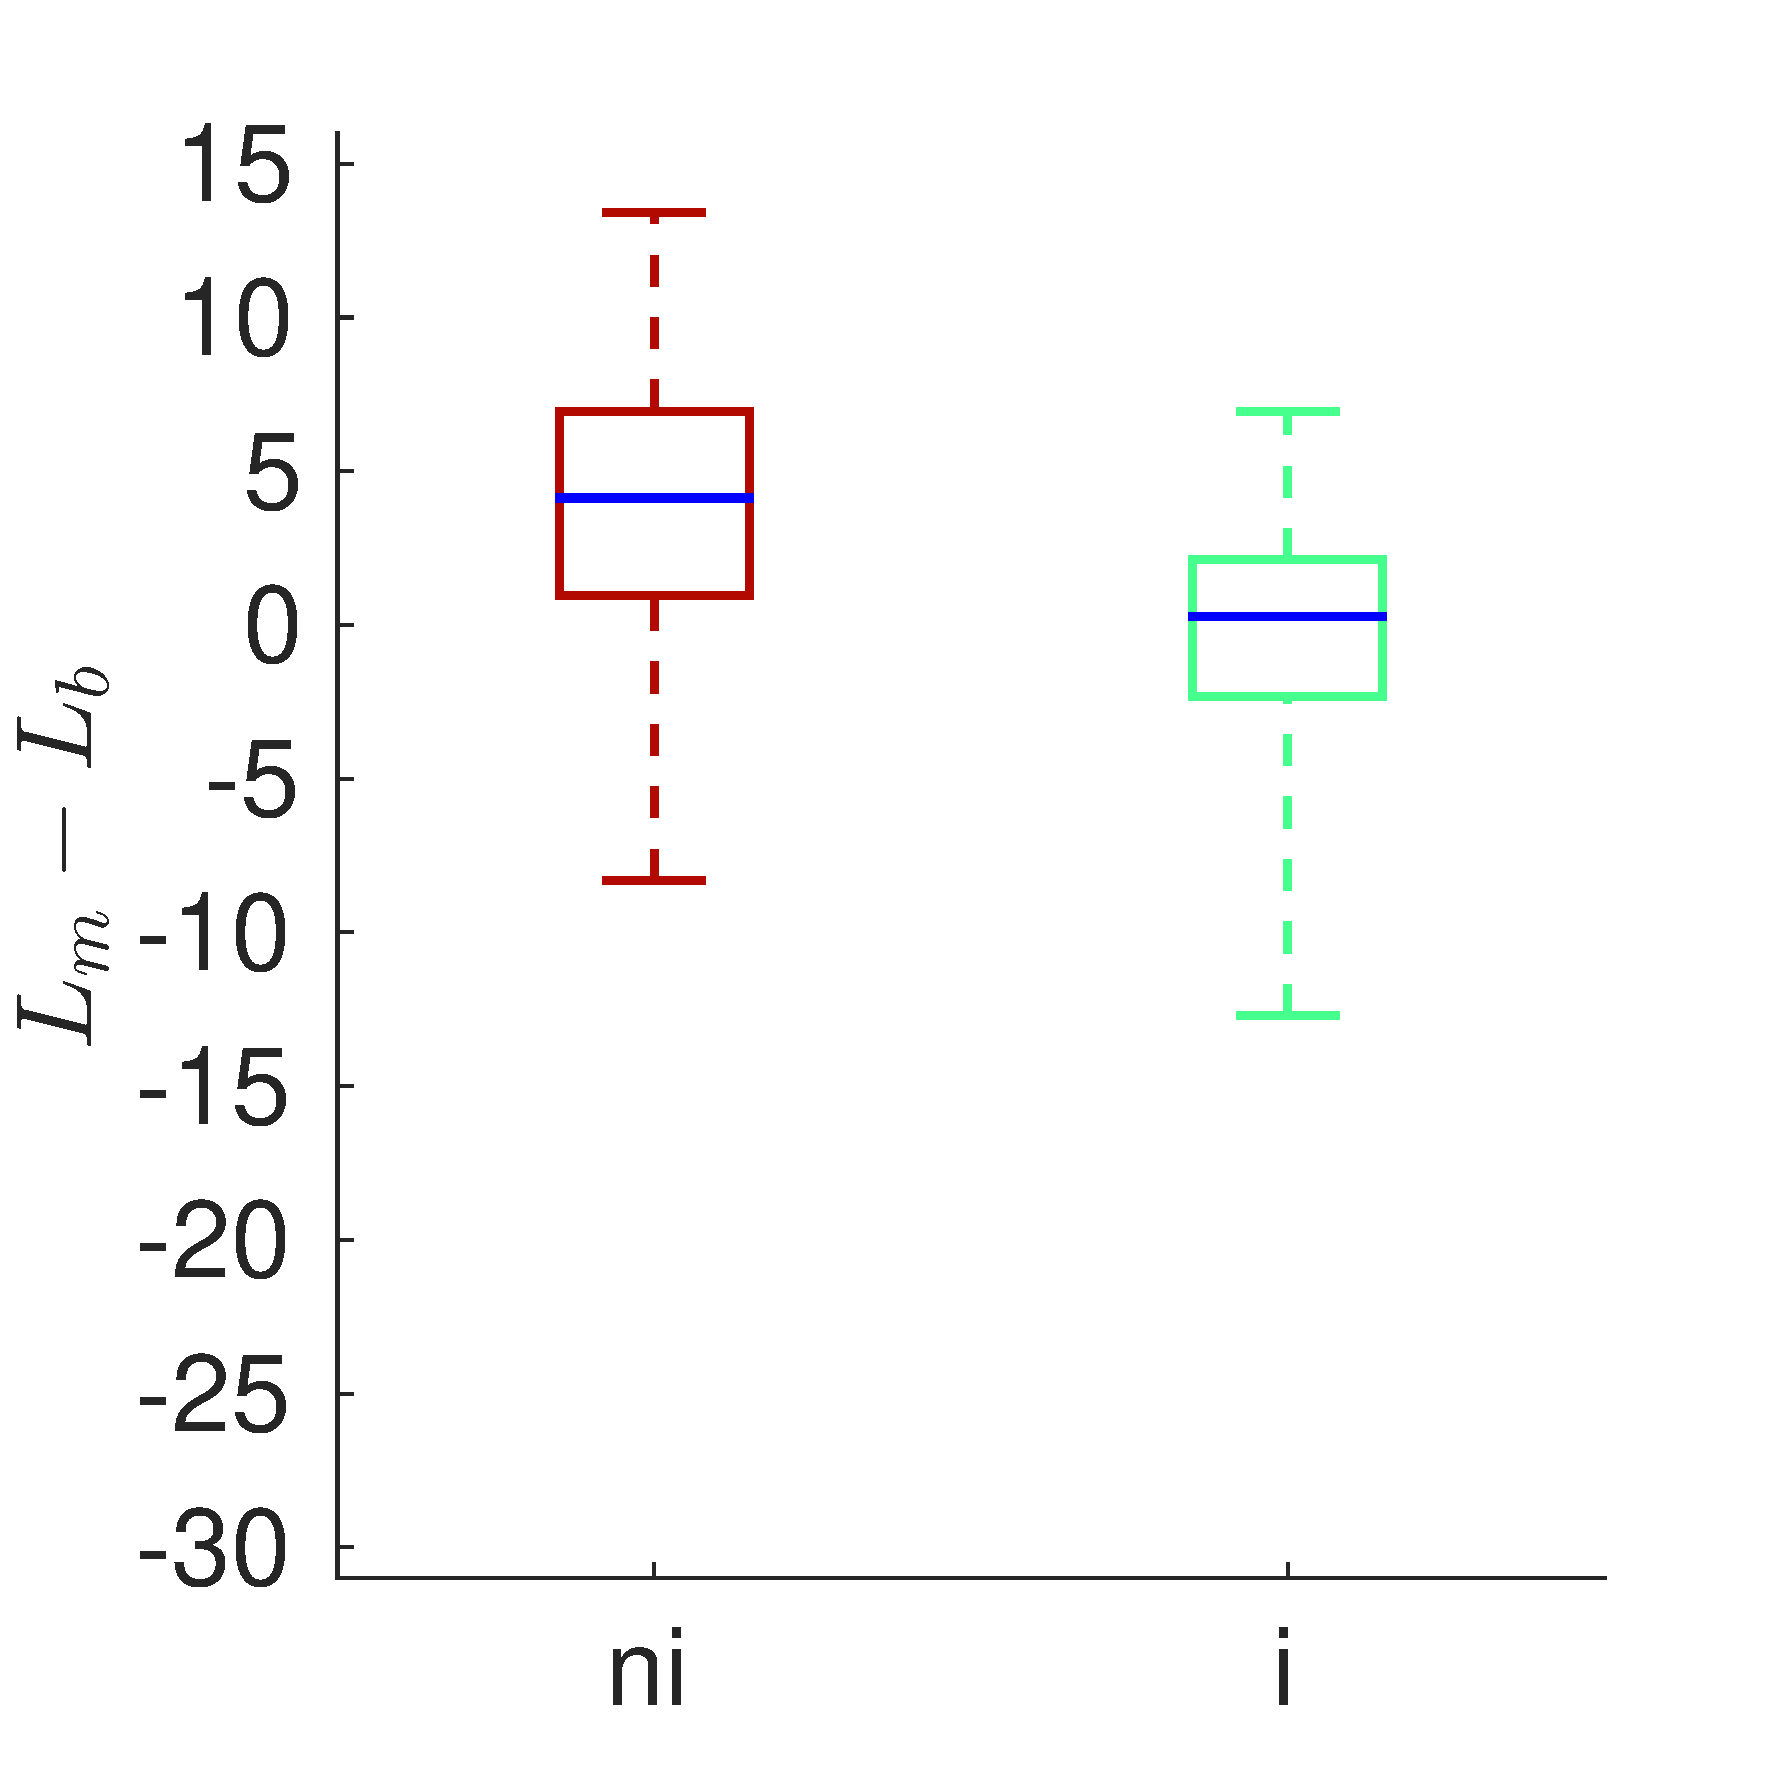
\includegraphics[width=.33\linewidth]{gfx/ch_5/xp_soundlevel_19}\label{fig:soundlevelMarkerDiffa}}
        \subfloat[]
        {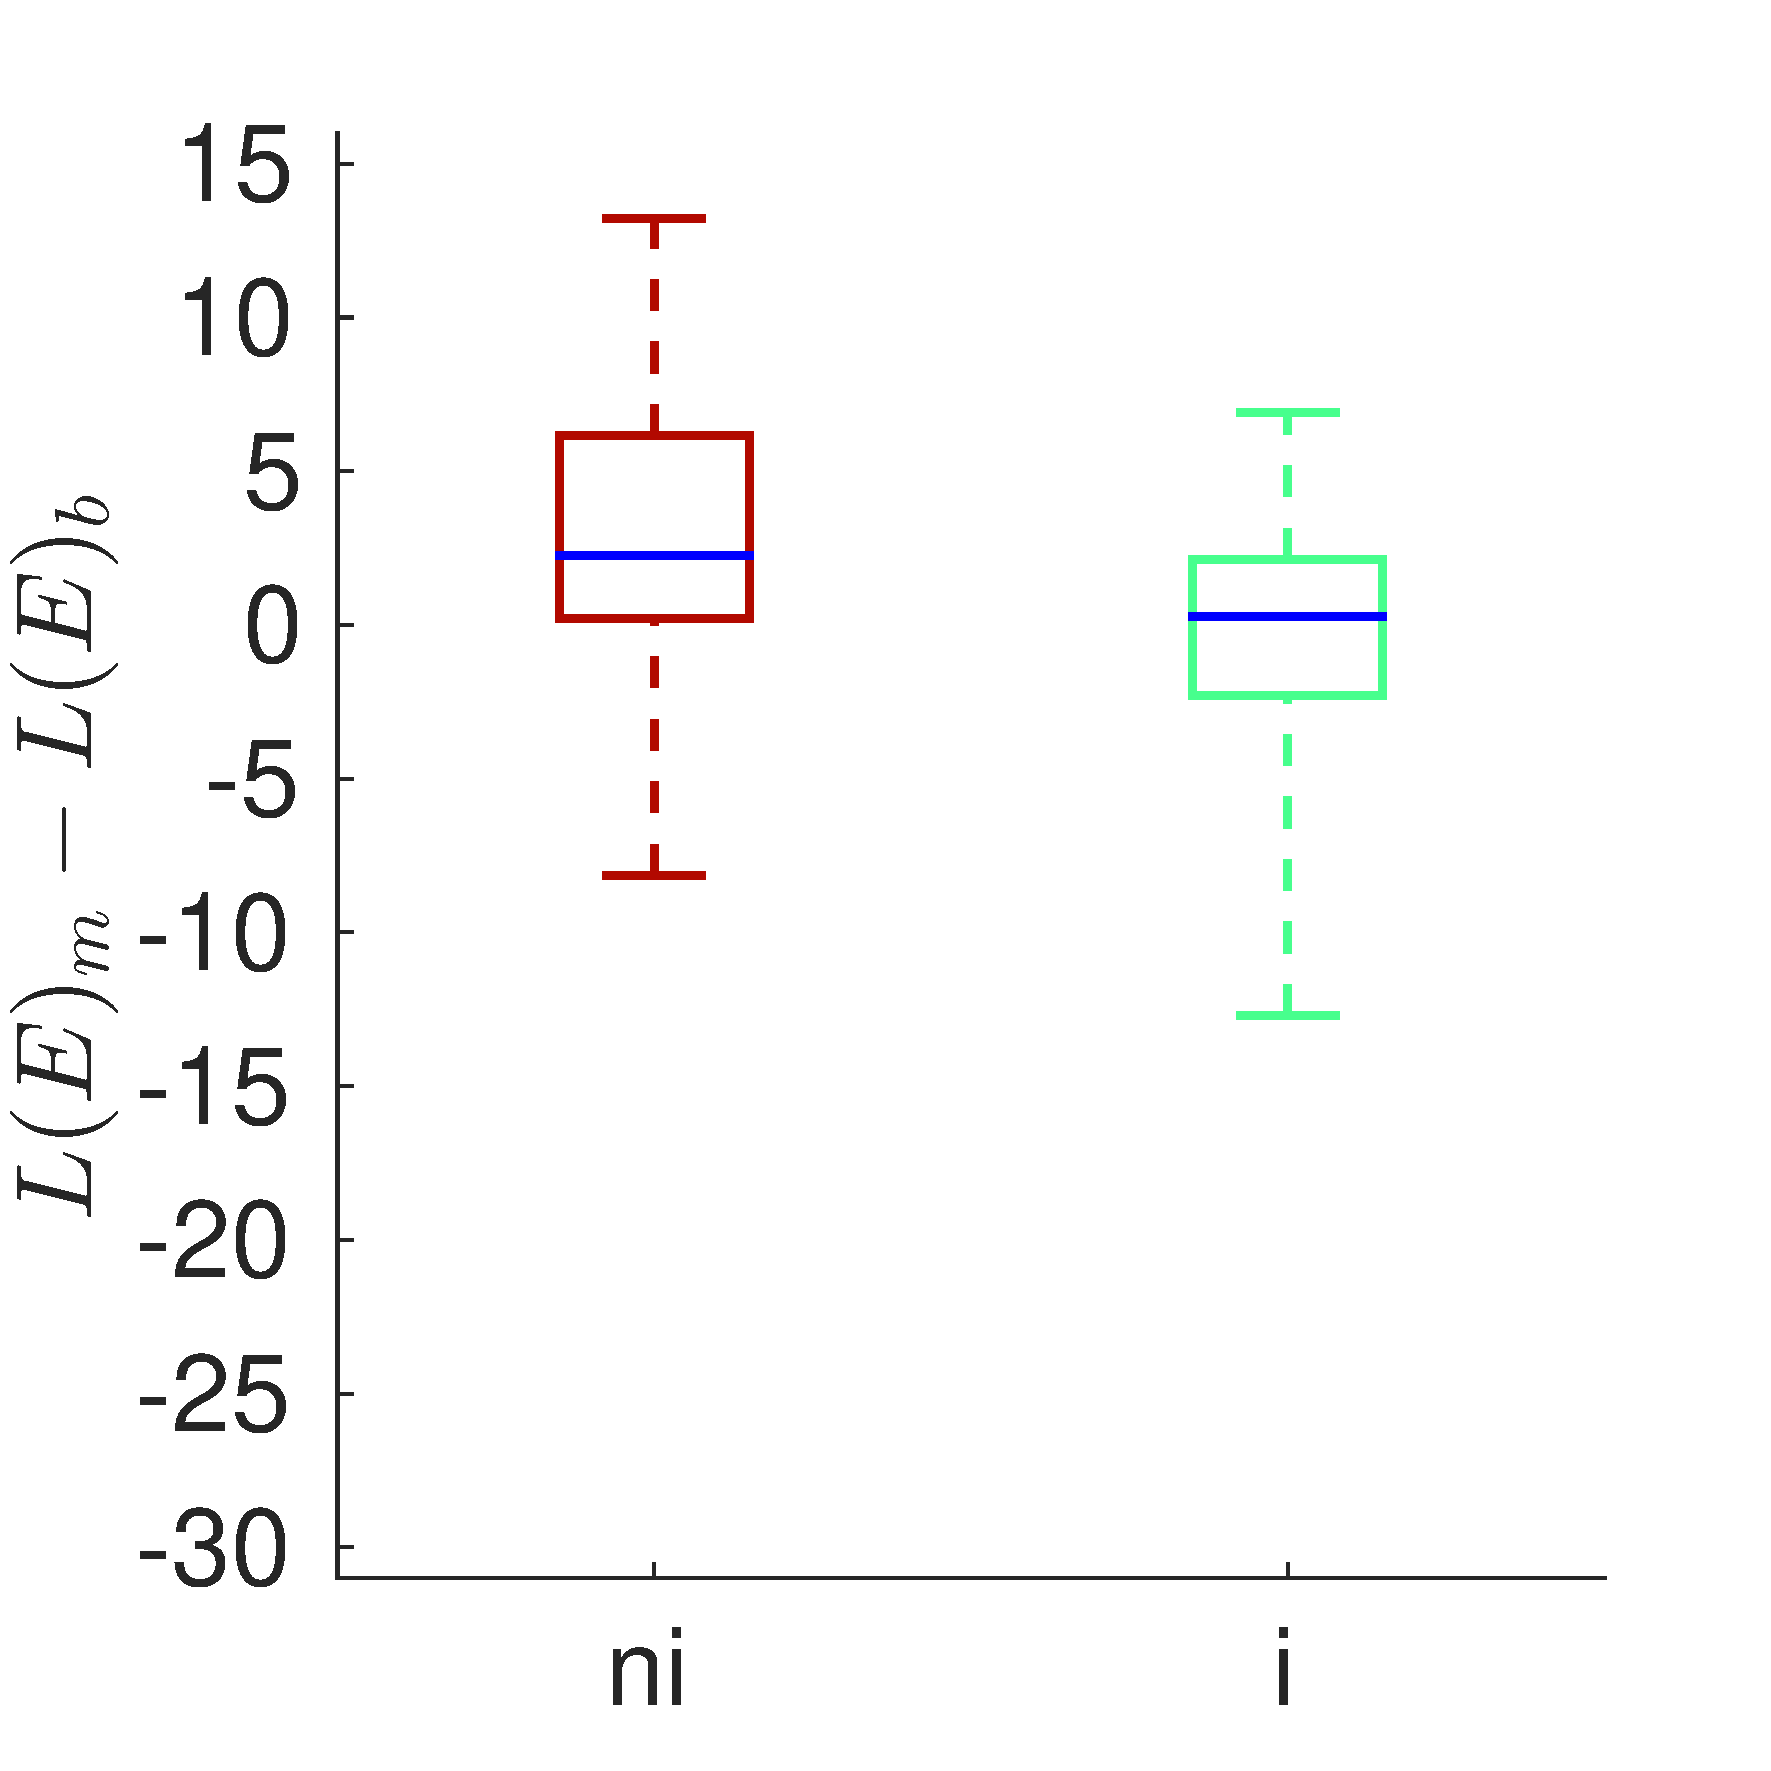
\includegraphics[width=.33\linewidth]{gfx/ch_5/xp_soundlevel_21}\label{fig:soundlevelMarkerDiffb}}
        \subfloat[]
        {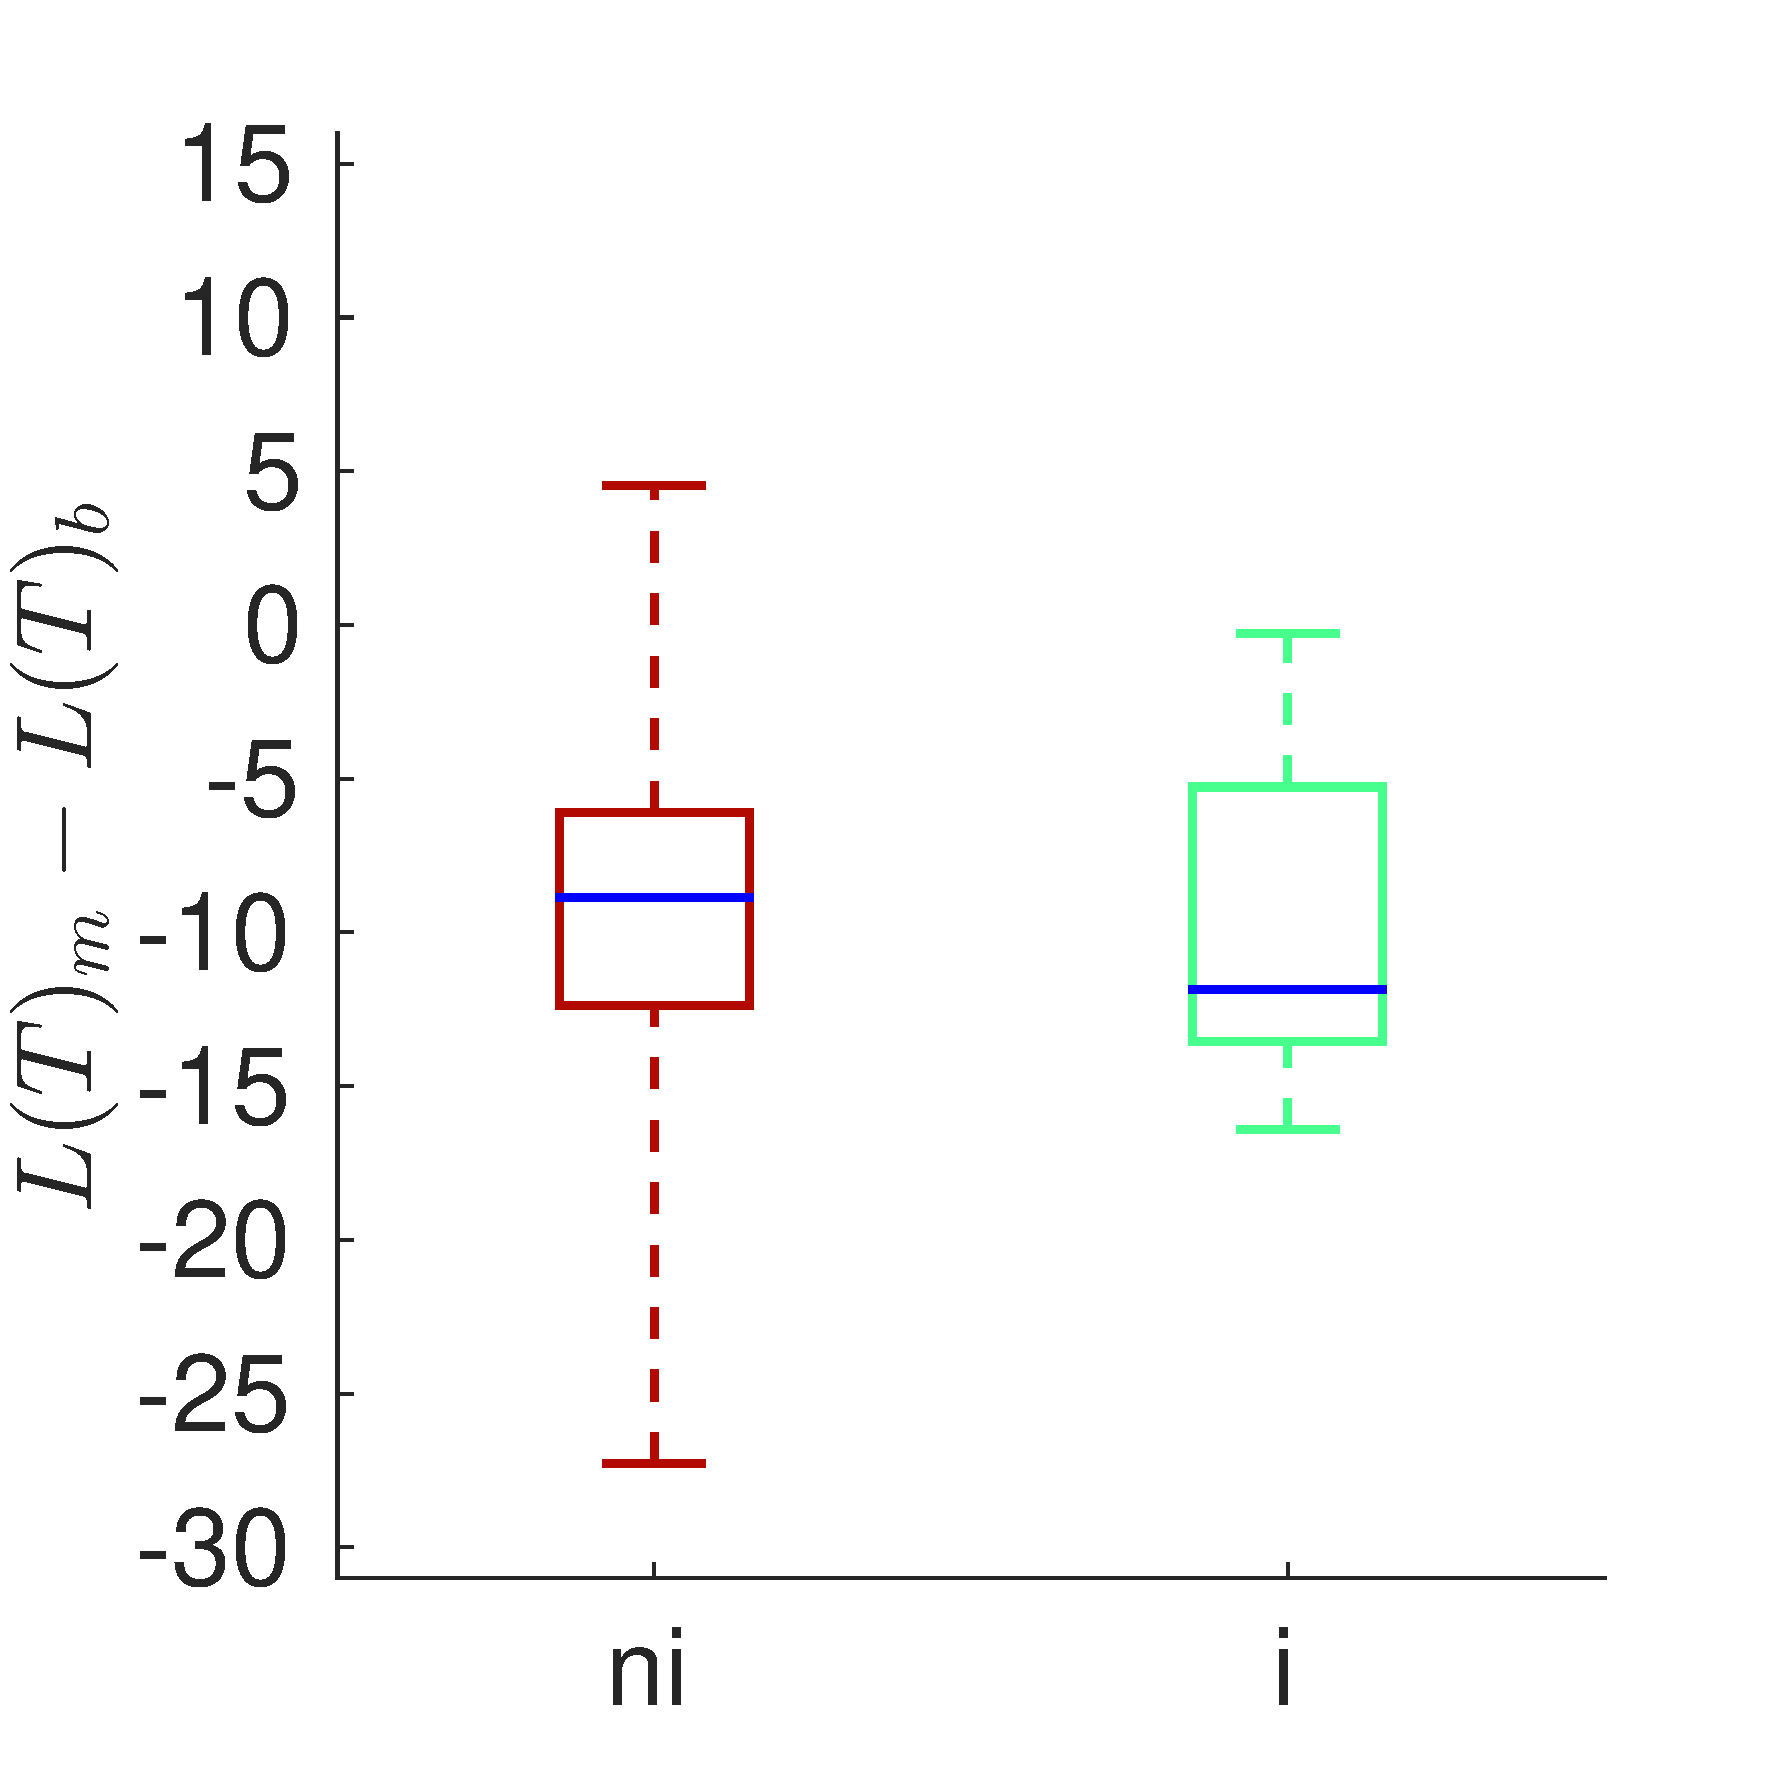
\includegraphics[width=.33\linewidth]{gfx/ch_5/xp_soundlevel_23}\label{fig:soundlevelMarkerDiffc}}\par
        \subfloat[]
        {\includegraphics[width=.33\linewidth]{gfx/ch_5/xp_soundlevel_20}\label{fig:soundlevelMarkerDiffd}}
        \subfloat[]
        {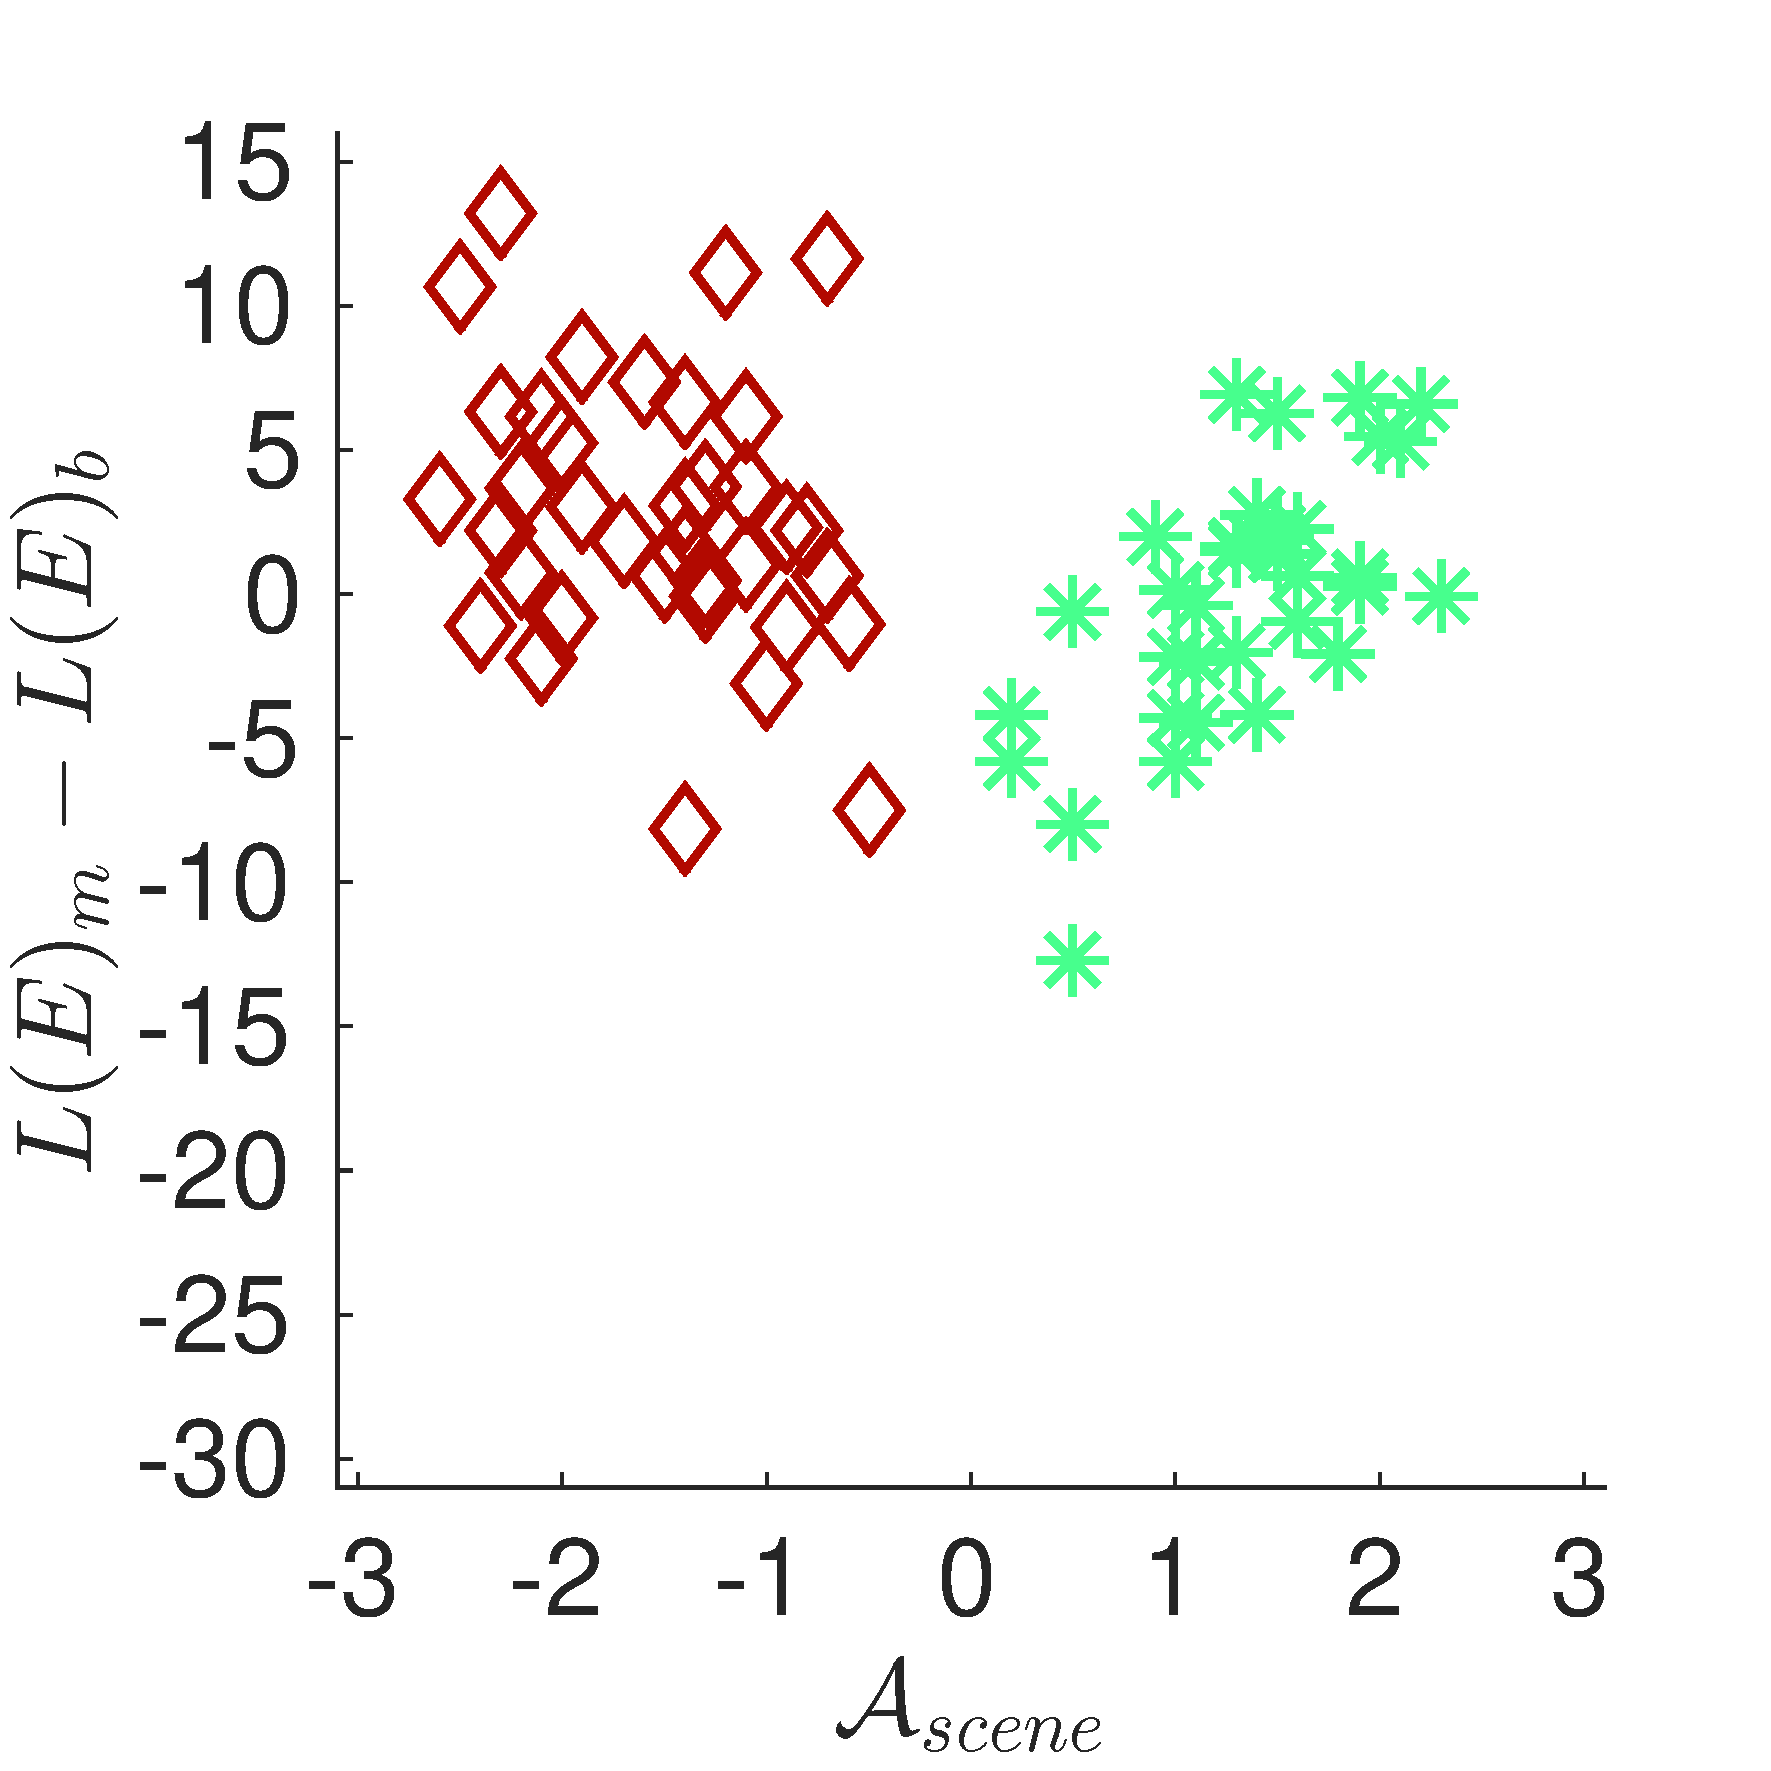
\includegraphics[width=.33\linewidth]{gfx/ch_5/xp_soundlevel_22}\label{fig:soundlevelMarkerDiffe}}
        \subfloat[]
        {\includegraphics[width=.33\linewidth]{gfx/ch_5/xp_soundlevel_24}\label{fig:soundlevelMarkerDifff}}
       \caption{Dispersions des descripteurs structurels de niveaux sonores relatifs à la présence des marqueurs $L_m-L_b$ (a, d), $L(E)_m-L(E)_b$ (b, e) et $L(T)_m-L(T)_b$ (c, f), en fonction du type de scènes (a, b, c) et de l'agrément perçu $\mathcal{A}_{scene}$ de l'expérience 1.b (d, e, f).}\label{fig:soundlevelMarkerDiff}
\end{figure}

\subsection{Discussions}

Dans cette expérience, nous identifions 6 indicateurs structurels globaux permettant de distinguer les environnements sonores idéaux et non-idéaux.

\begin{itemize}
\item niveau sonore: calculé sur tous les sons $L$, les événements $L(E)$ et les textures $L(T)$; 
\item densité: calculée de manière globale $D$ et sur les événements $D(E)$;
\item diversité: calculée uniquement sur les événements $DIV(E)$.
\end{itemize}

Parmi ces indicateurs structurels, seuls $L$ et $LE$ permettent de prédire l'agrément. Nous notons cependant que cette prédiction ne vaut que pour les ni-scènes. 

Nous observons qu'une description sémantique des scènes, basée sur la présence/absence des classes de sons, permet de bien prédire la nature de l'environnement. Par ailleurs, il apparaît qu'il est possible d'obtenir une prédiction similaire, voire meilleure, en ne considérant qu'un sous groupe de classes d'événements,\ie~les marqueurs sonores.

Parmi les descripteurs structurels spécifiques, calculés en tenant compte des marqueurs sonores, plusieurs permettent maintenant de faire la distinction entre les i-scènes et ni-scènes:

\begin{itemize}
\item niveau sonore: $L_m$, $L_{b}$, $L(E)_{m}$, $L(E)_{b}$, $L(T)_{m}$, $L(T)_{b}$, $L_{m}-L_{b}$ et $L(E)_{m}-L(E)_{b}$;
\item densité: $D_{m}$.
\end{itemize}

Parmi ces descripteurs, 8 semblent impacter l'agrément perçu: 

\begin{itemize}
\item $L_b$ et $L(E)_b$ ont un impact négatif sur les i-scènes;
\item $L(E)_m-L(E)_b$ et $L_m-L_b$ ont un impact positif sur les i-scènes;
\item $L_m$, $L(E)_m$, $L(T)_b$ et $D(E)_m$ ont un impact négatif les ni-scènes.
\end{itemize}

De cette analyse, nous retenons les points suivants:

\begin{itemize}
\item \emph{distinguer les i- et ni-scènes}: les descripteurs sémantiques, ainsi que certains descripteurs structurels globaux, permettent de faire la distinction entre les i-scènes et les ni-scènes. La description sémantique semble être plus performante;
\item \emph{événements ou textures}: que ce soit pour les descripteurs sémantiques ou structurels, ce sont majoritairement les événements qui permettent de distinguer les deux types d'environnements, les textures n'apportant, au mieux, qu'une information limitée;
\item \emph{prédire l'agrément}: si l'on considère une description fine de l'agrément, il semble que la manière de percevoir la qualité de l'environnement diffère en fonction de la nature de ce dernier (i ou ni). Il n'apparaît pas envisageable de considérer un même jeu de descripteurs pour prédire, à la fois, l'agrément des i-scènes, et l'agrément des ni-scènes. Pour les ni-scènes, ce sont le niveau global ($L$ et $L(E)$), la densité globale ($D$ et $D(E)$), ou le niveau des marqueurs sonores ($L_m$ et $L$), qui impactent négativement l'agrément. On note ici que prendre en compte les contributions de différentes sources n'améliore pas la capacité de prédiction de l'agrément, par rapport à une analyse holistique de l'environnement. Pour les i-scènes, par contre, prédire l'agrément requiert d'étudier, de manière séparée, les caractéristiques des marqueurs sonores, et celles de l'ensemble des autres sons. Ainsi, le niveau des marqueurs relatifs au bruit est positivement corrélé à l'agrément, alors que le niveau du bruit est, lui, négativement corrélé.  
\end{itemize}

Le fait que l'agrément des scènes agréables ne se corrèlent pas avec des descripteurs physique holistiques, contrairement à l'agrément des scènes désagréable, a récemment été déjà observé \citep{gozalo2015relationship}.

L'existence de deux modes de perception, mobilisant différents types de descripteurs, et dépendant de la nature (dans notre cas hédonique) des stimuli, est un phénomène qui se rapproche de celui observé pour la perception des textures (\cf~Section~\ref{sec:ch3_eventTexture}). Le cerveau adapte sa manière de traiter l'information (résumé statistique pour les textures, description fine pour les événements) suite à une prise de décision antérieure quant à la nature du stimulus (à savoir « est-ce un événement ou une texture ? »). De la même manière, les indicateurs actifs dans le jugement de l'agrément dépendent, eux aussi, d'une identification préalable de la nature hédonique globale de l'environnement (idéale ou non idéale).

Ces résultats peuvent potentiellement influer sur les stratégies à adopter pour améliorer la qualité de l’environnement sonore:

\begin{itemize}
\item dans le cadre de scènes non-idéales, il s'agit de diminuer le niveau sonore, soit de manière globale, soit en agissant sur certaines sources (\emph{sirène}, \emph{klaxon});
\item dans le cadre de scènes idéales, il s'agit 1) d'identifier les sons agréables, \ie~les marqueurs sonores, 2) de baisser le niveau des autres sons, 3) voire, en restant dans la limite du raisonnable, d'augmenter le niveau des marqueurs par rapport aux autres sons.
\end{itemize}

Nous montrons que les descripteurs à utiliser dépendent de la nature de l'environnement, et que cette nature est elle même dépendante de la composition sémantique, \ie~des sources sonores présentes. Dans une certaine mesure, nous pouvons donc dire que les descripteurs dépendent des sources sonores présentes. 

%\gl{TODO: "Mais nous observons également que le type de descripteurs à utiliser, pour une même source, varie en fonction de la nature de l'environnement." : développer sur le contexte environnemental pour l'agrément, reprendre l'exemple de \emph{foule}} \\
%\gl{TODO: Reprendre la conclusion de l'article et Proposer un modèle perceptif sur la base du modèle prédictif}\\
%\gl{TODO, l'utilisation de trafic reprendre les conclusions de \citep{lavandier2006contribution}}\\
%\gl{TODO, les résultats (2 modes d'obs) concordent avec les observations faites pas \citep{ricciardi2015sound}.}\\

%%%%%%%%%%%%%%%%%%%%%%%%%%%%%%%%%%%%%%%%%%%%%%%%%%%%%%%%%%%%%%%%%%%%%%%
%%%%%%%%%%%%%%%%%%%%%%%%%%% XP 2 %%%%%%%%%%%%%%%%%%%%%%%%%%%%%%%%%%%%%%
%%%%%%%%%%%%%%%%%%%%%%%%%%%%%%%%%%%%%%%%%%%%%%%%%%%%%%%%%%%%%%%%%%%%%%%

\section[Modification de la composition sémantique]{Agir sur l'agrément perçu en modifiant la composition sémantique}
\label{sec:xp3}

\subsection{Objectif}

L'expérience précédente à montré que, parmi les classes de sons peuplant le monde sonore, celles regroupant les marqueurs sont caractéristiques de certains types d'environnements. Ces marqueurs sonores semblent avoir un impact particulier sur la perception de leurs environnements. C'est ce dernier point qui est étudié dans cette expérience.

Afin de vérifier que l'agrément des scènes idéales et non-idéales dépend de la présence des marqueurs, les scènes sonores précédemment simulées sont régénérées, sans les classes de marqueurs. Pour les i-scènes, les i-marqueurs sont retirés. Pour les ni-scènes, les ni-marqueurs. Une épreuve d'évaluation de l'agrément, dont le protocole se rapproche de celui de l'expérience 1.b, est alors conduite.

L'objectif est de vérifier si l'absence des marqueurs a un impact sur l'agrément perçu. Deux hypothèses sont formulées:

\begin{itemize}
\item \emph{pour les ni-scènes} nous faisons l'hypothèse que l'absence des ni-marqueurs va \textbf{augmenter} la valeur de l'agrément perçu;
\item \emph{pour les i-scènes} nous faisons l'hypothèse que l'absence des i-marqueurs va \textbf{diminuer} la valeur de l'agrément perçu.
\end{itemize}

Si la première hypothèse est intuitive, la deuxième l'est moins. En effet, il n’apparaît pas évident que la suppression des i-marqueurs, bien que s'agissant de sons positivement connotés, diminue la qualité globale d'un environnement. Cette suppression aura, de surcroît, pour effet de diminuer le niveau sonore global de la scène. 

Néanmoins, comme nous l'avons vu, le niveau global n'est qu'un indicateur partiel de l'agrément pour les environnements sonores idéaux. Qui plus est, cet indicateur, lorsque qu'il décrit le niveau des i-marqueurs, impacte de manière positive la qualité de la scène. L'hypothèse mérite donc d'être vérifiée.

\subsection{Planification expérimentale}

Nous nommons cette expérience: \emph{expérience 2}. \\

{\setlength{\parindent}{0cm}\textbf{Banque de données}} \\

La banque de données de stimuli compte 144 séquences de 30 secondes. Ces 144 séquences comprennent:

\begin{itemize}
\item \emph{72 am-scènes}: les 72 scènes précédemment simulées, incluant les classes de marqueurs (am). Nous notons i/am-scenes, les 36 scènes idéales avec marqueurs, et ni/am-scènes les 36 scènes non-idéales avec marqueurs;
\item \emph{72 sm-scènes}: les 72 scènes précédemment simulées, régénérées sans les classes de marqueurs (sm). Nous notons i/sm-scenes, les 36 scènes idéales sans marqueurs, et ni/sm-scènes les 36 scènes non-idéales sans marqueurs.
\end{itemize}

Nonobstant l'absence des marqueurs, les am- et sm-scènes sont en tout point semblables. 

Nombre de am-scènes sont composées, en majorité, de samples de marqueurs. Afin de pas abusivement dénaturer ces scènes, en créant notamment des temps de « vide », \ie~ne comprenant aucun sample, nous ne supprimons que les marqueurs des classes d'événements du premier niveau d'abstraction (\cf~Tableau~\ref{tab:markers}). Ces classes sont: 

\begin{itemize}
\item \emph{cloche}, \emph{sonnette de vélo}, \emph{animaux} pour les i/sm-scenes;
\item \emph{sirène}, \emph{klaxon} pour les ni/sm-scenes.
\end{itemize}
 
Il est important de noter ici que tous les i- et ni-marqueurs ne sont donc pas supprimés dans les sm-scènes. \\
 
{\setlength{\parindent}{0cm}\textbf{Procédure}} \\

Les sujets évaluent les 144 scènes. L'évaluation s'effectue sur une échelle sémantique bipolaire de 11 points allant de -5 (non-idéale/très désagréable) à +5 (idéale/très agréable). Avant de noter une scène, les sujets doivent obligatoirement en écouter les 20 premières secondes. Après la notation, ils sont libres de passer à la scène suivante.

Pour chaque sujet, les scènes sont présentées dans un ordre aléatoire. Les 10 premières scènes permettent au sujet de calibrer ses notes. Elles sont obligatoirement composées de 5 i/am-scènes et de 5 ni/am-scènes. Ces 10 premières scènes sont rejouées à la fin de l'expérience, et seules les notes données à la deuxième occurrence sont prises en compte. 

L'expérience est prévue pour durer 1 heure. Les sujets ne connaissent pas la nature des scènes.\\

{\setlength{\parindent}{0cm}\textbf{Dispositif expérimental}} \\

Tous les sujets passent l'expérience sur des machines identiques. L'audio est diffusé en monophonie, par le biais de casques audio semi-ouverts \emph{Beyer-Dynamic DT 990 Pro}. Toutes les scènes sonores ont été re-simulées sur la base des partitions obtenues lors de l'expérience de simulation. Le niveau sonore de sortie est identique pour tous les sujets.

%\gl{TODO: description des machines}
 
Tous les sujets réalisent l'expérience simultanément, dans un environnement calme. Ils n'ont pas le droit de s'adresser la parole pendant l'expérience. 

Un expérimentateur est présent durant la totalité de l'expérience, afin de contrôler le bon déroulement de cette dernière, et de répondre aux éventuelles questions des sujets.  \\

{\setlength{\parindent}{0cm}\textbf{Participants}} \\

12 sujets (4 femmes) participent à l'expérience. Aucun d'entre eux n'a réalisé l'expérience de simulation, ni la première expérience d'évaluation. Les sujets sont âgés de 22 à 61 ans (moyenne: 29.5, écart-type: 14). Tous les sujets vivent dans un milieu urbain.

Tous les sujets ont réalisé l'expérience avec succès.

\subsection{Données et méthodes d'analyses}

\subsubsection{Nature des données analysées}

Les données analysées sont les mêmes que pour la première expérience. Nous invitons le lecteur à se référer à la section~\ref{sec:ch5_dataType1} pour plus de détails.
 
\subsubsection{Méthodologie et Outils statistiques}
\label{sec:ch5_methodoEtStat2}

L'expérience aborde trois problématiques:

\begin{itemize}
\item \emph{influence des descripteurs structurels des scènes avec marqueurs sur l'agrément perçu: une analyse comparative}: les 72 am-scènes utilisées par l'expérience 1.b étant ré-évaluées lors de cette expérience, il est donc possible de réaliser une étude comparative entre les expériences 1.b et 2, afin de vérifier la cohérence des résultats obtenus lors de l'expérience 1.b. Les méthodes d'analyse appliquées sont identiques à celles de l'expérience 1.b (\cf~Section~\ref{sec:ch5_methodoEtStat1});
\item \emph{influence de la présence des marqueurs sur l'agrément perçu}: il s'agit ici de vérifier que la suppression des i- et ni-marqueurs impacte l'agrément perçu. Pour ce faire, nous utilisons l'analyse de variance (\cf~Annexe~\ref{app:anova}). Nous considérons, comme variable dépendante,  $\mathcal{A}_{sujet}$, et, comme variables indépendantes, le type d'environnement (i/ni), et la présence/absence de marqueurs (am/sm). Chaque sujet devant évaluer la totalité des stimuli, une ANOVA à mesures répétées à deux facteurs (\cf~Annexe~\ref{app:anova}) est utilisée afin vérifier s'il existe des différences significatives d'agrément perçu. Les deux variables indépendantes sont considérées comme des facteurs intra-sujet (\emph{within-subject}, \cf~Annexe~\ref{app:anova}). Les facteurs n'étant composés que de deux niveaux chacun (type: i/ni; marqueur: am/sm), l'hypothèse de sphéricité n'a pas besoin d'être vérifiée. Les analyses \emph{post hoc} sont conduites en appliquant la procédure de Tukey-Kramer (\cf~Annexe~\ref{app:anova});
\item \emph{influence des descripteurs structurels des sm-scènes sur l'agrément perçu}: il s'agit là d'étudier l'agrément en fonction des indicateurs structurels des scènes. Dans un premier temps, nous vérifions que l'agrément moyen de chaque type de scènes (i, ni, am et sm) varie significativement. Une analyse de variance est pratiquée, avec, comme variable dépendante, $\mathcal{A}_{scene}$, et, comme variables indépendantes, le type d'environnement (i/ni), et la présence/absence de marqueurs (am/sm). Dans cette analyse, les observations considérées sont les scènes. Comme il existe une dépendance entre les am et sm-scènes, une ANOVA à mesures répétées est utilisée, comprenant, comme facteur intra-sujet (\emph{within-subject}), la présence/absence de marqueurs, et comme facteur inter-sujet (\emph{between-subject}), le type d'environnement. Les analyses \emph{post hoc} sont conduites en appliquant la procédure de Tukey-Kramer. Dans un second temps, comme pour l'expérience 1.b, nous étudions l'existence de relations linéaires entre les descripteurs structurels des sm-scènes et $\mathcal{A}_{scene}$. Pour mesurer la corrélation, nous utilisons le coefficient de Pearson (\cf~Annexe~\ref{app:statuni}).
\end{itemize}

Tous les tests de significativité sont effectués avec un seuil critique $\alpha=0.05$.

\subsection{Détection de valeurs extrêmes}

Considérons $\mathcal{A}_{sujet}$ pour les am-scènes (\cf~Figure~\ref{fig:xp4_note_2}). Il apparaît que les réponses du sujet 7 diffèrent des autres. Comme observé sur la figure~\ref{fig:xp4_note_1} (\cf~Figure~\ref{fig:xp4_note_1g} pour le sujet 7), ce dernier a évalué positivement près de la moitié des ni/am-scènes. Le sujet 7 a donné à 58\% des ni/am-scènes une note supérieure à 0, contre une moyenne de 11\% pour les autres sujets. De plus, le sujet 7 a utilisé l'ambitus maximal (-5 à 5) pour noter à la fois les i/ et ni/am-scènes. Ces faits n'ayant pas été observés pour les autres sujets, que l'on considère les expériences 2 ou 1.b, le sujet 7 est éliminé de l'analyse. 

\begin{figure}[t]
        \myfloatalign
        \subfloat[sujet 1]
        {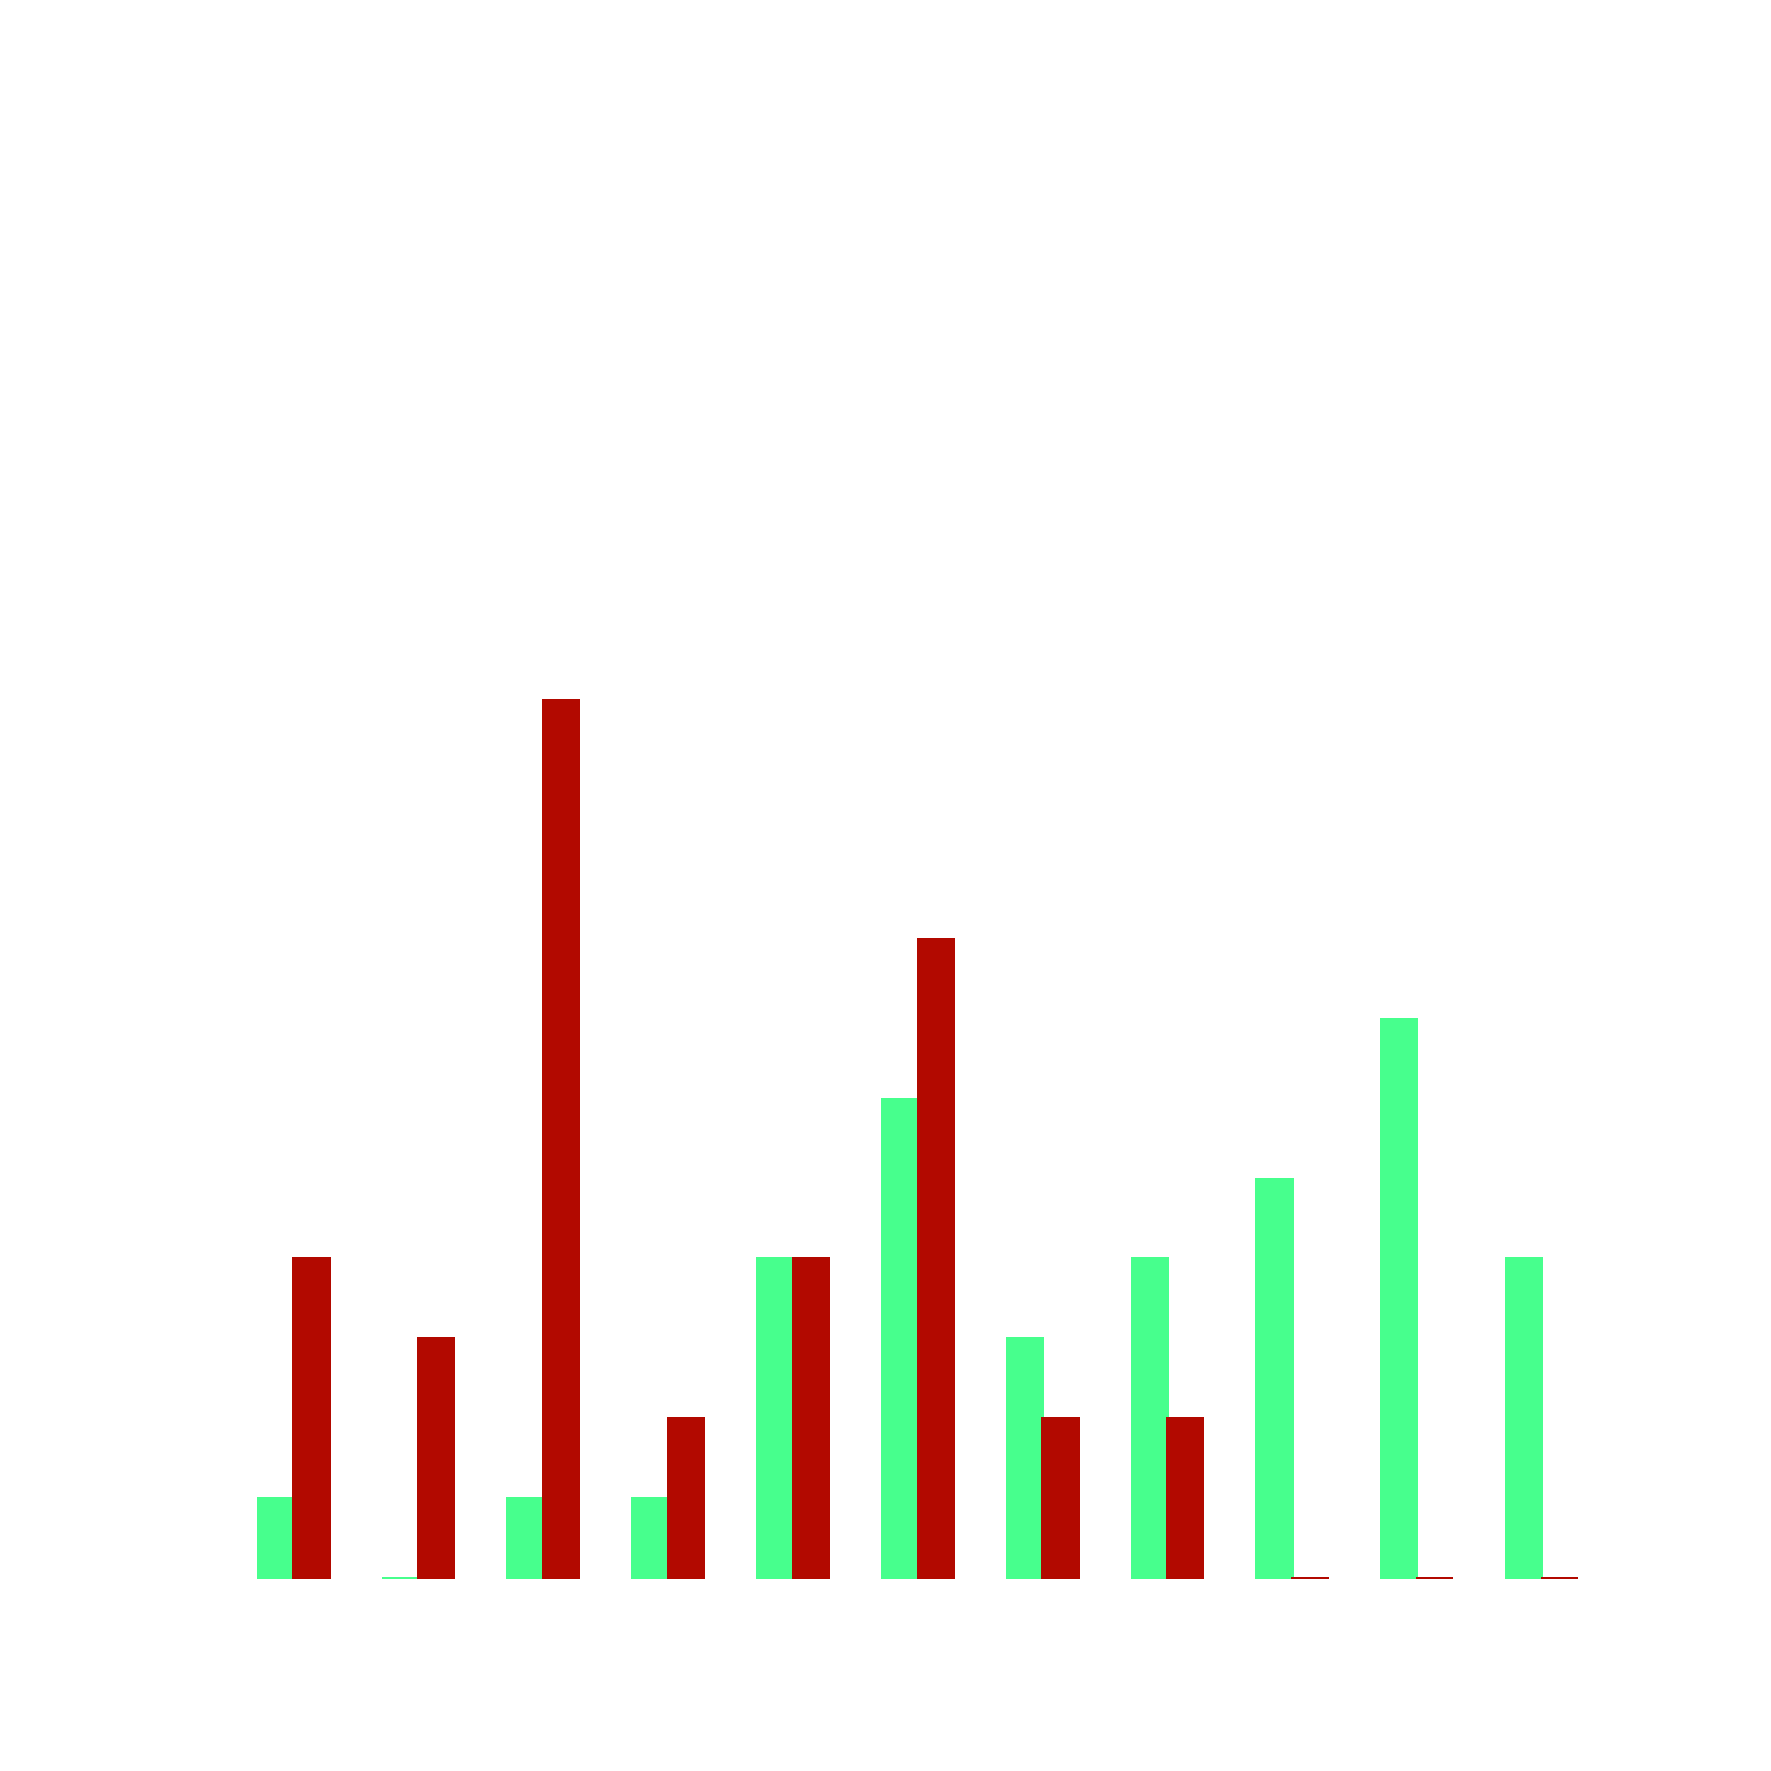
\includegraphics[width=.16\linewidth]{gfx/ch_5/xp4_note_1}\label{fig:xp4_note_1a}}
        \subfloat[sujet 2]
        {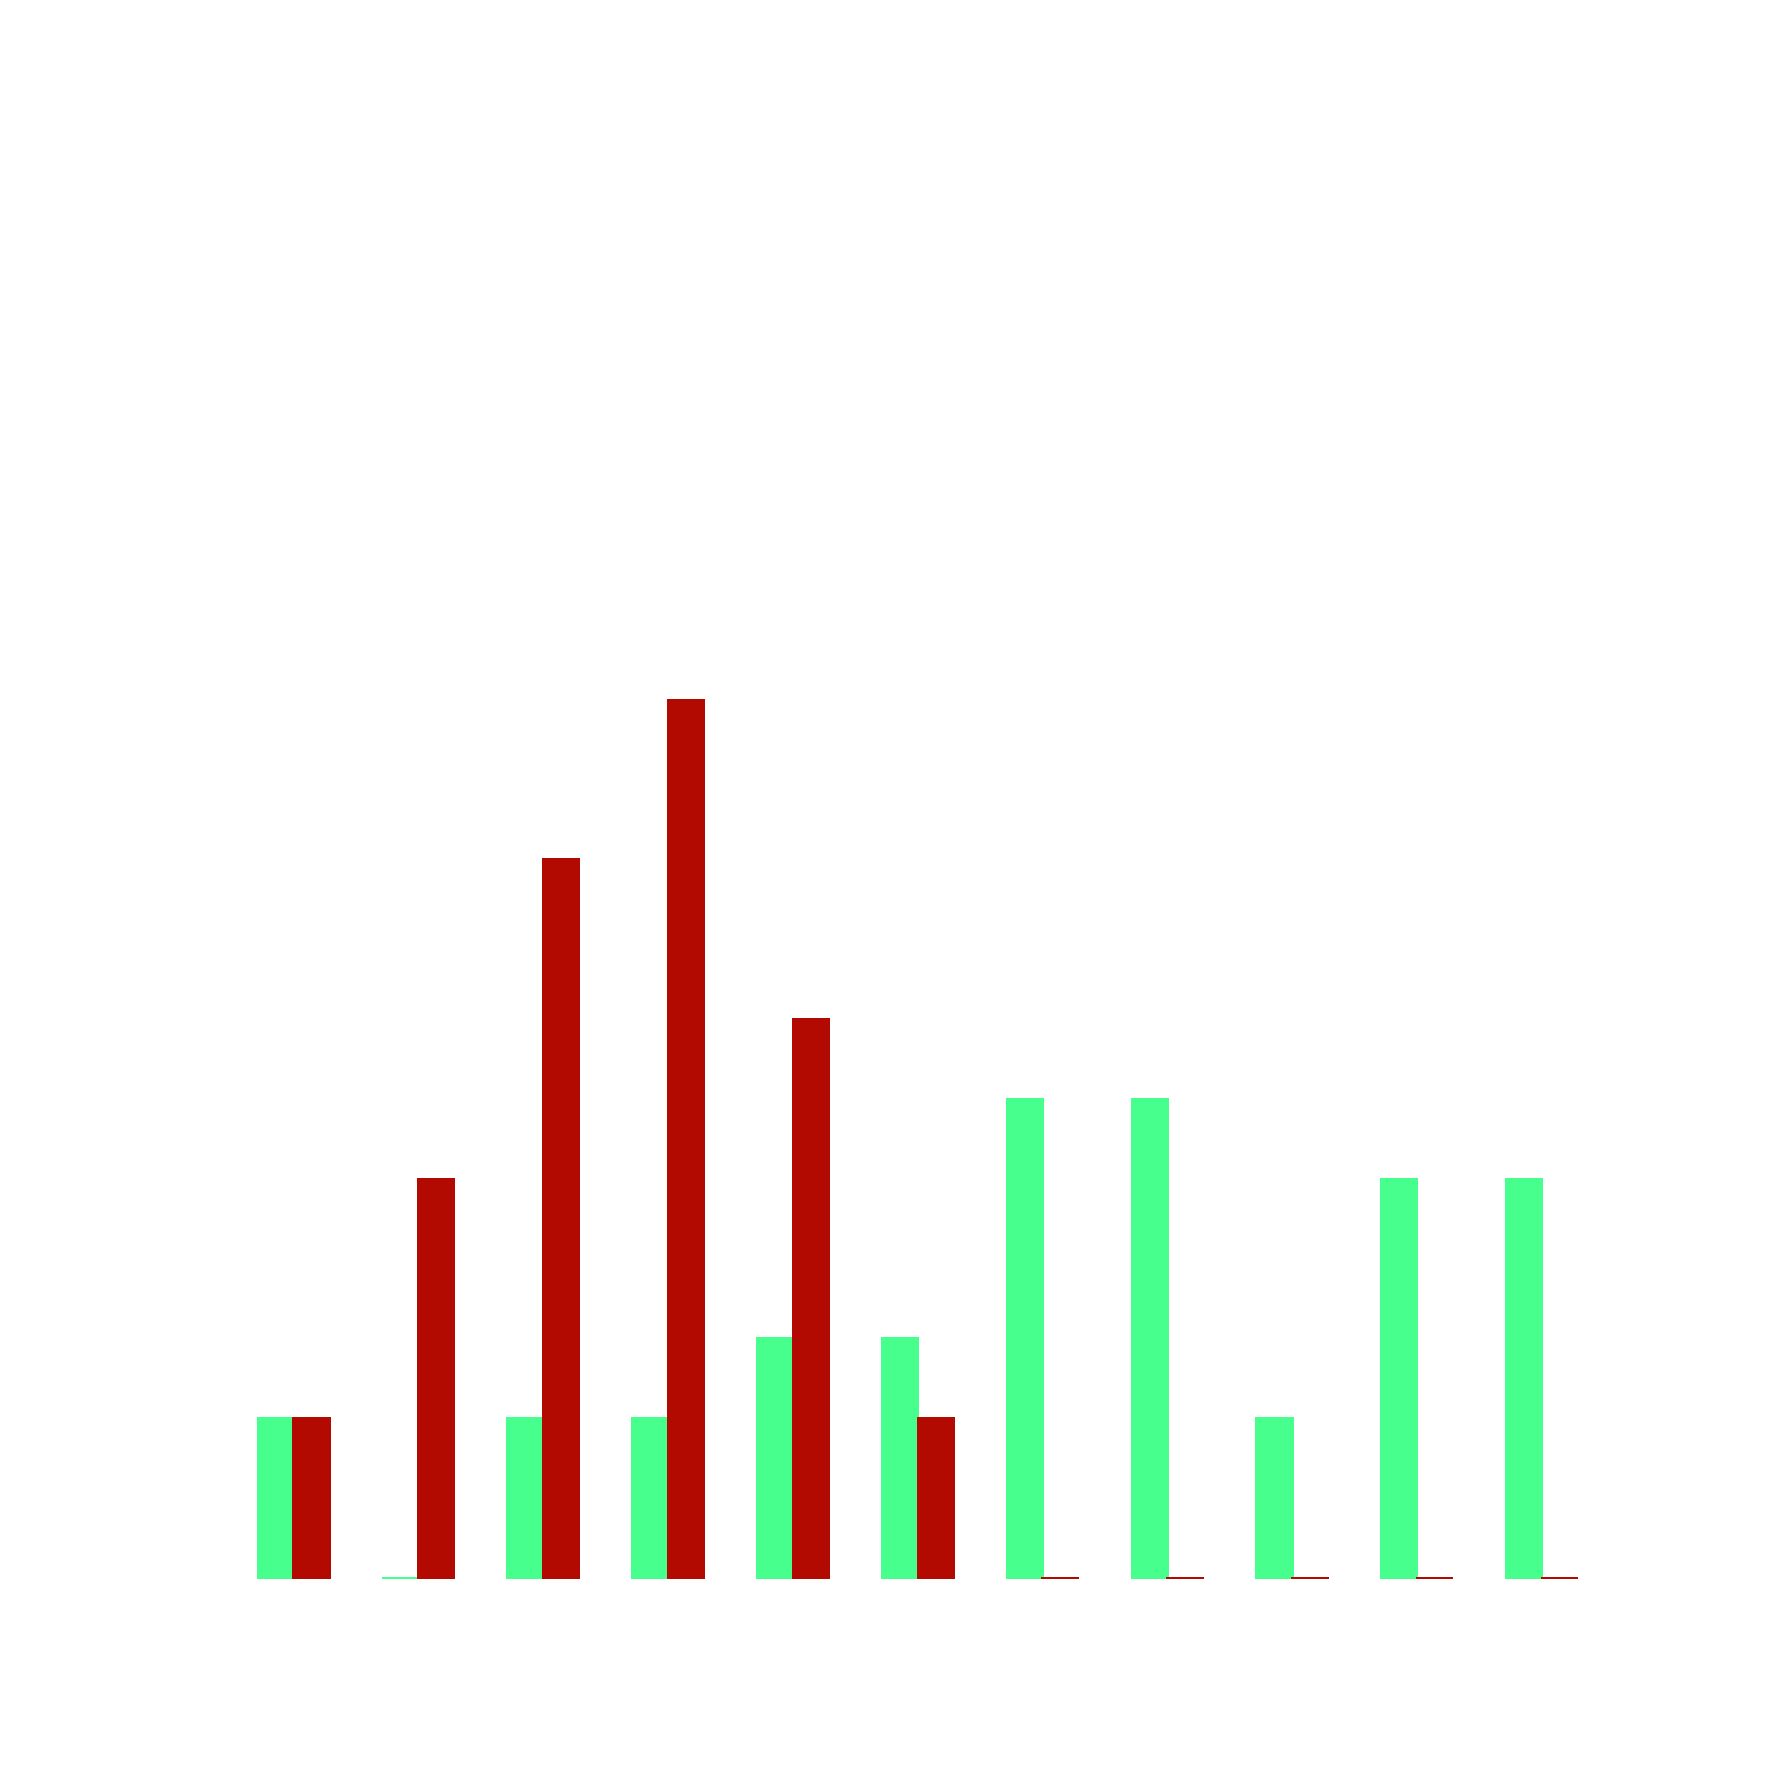
\includegraphics[width=.16\linewidth]{gfx/ch_5/xp4_note_2}\label{fig:xp4_note_1b}}
        \subfloat[sujet 3]
        {\includegraphics[width=.16\linewidth]{gfx/ch_5/xp4_note_3}\label{fig:xp4_note_1c}}
        \subfloat[sujet 4]
        {\includegraphics[width=.16\linewidth]{gfx/ch_5/xp4_note_4}\label{fig:xp4_note_1d}}
        \subfloat[sujet 5]
        {\includegraphics[width=.16\linewidth]{gfx/ch_5/xp4_note_5}\label{fig:xp4_note_1e}}
        \subfloat[sujet 6]
        {\includegraphics[width=.16\linewidth]{gfx/ch_5/xp4_note_6}\label{fig:xp4_note_1f}}\par       
        \subfloat[sujet 7]
        {\includegraphics[width=.16\linewidth]{gfx/ch_5/xp4_note_7}\label{fig:xp4_note_1g}}
        \subfloat[sujet 8]
        {\includegraphics[width=.16\linewidth]{gfx/ch_5/xp4_note_8}\label{fig:xp4_note_1h}}
        \subfloat[sujet 9]
        {\includegraphics[width=.16\linewidth]{gfx/ch_5/xp4_note_9}\label{fig:xp4_note_1i}}
        \subfloat[sujet 10]
        {\includegraphics[width=.16\linewidth]{gfx/ch_5/xp4_note_10}\label{fig:xp4_note_1j}}
        \subfloat[sujet 11]
        {\includegraphics[width=.16\linewidth]{gfx/ch_5/xp4_note_11}\label{fig:xp4_note_1h}}
        \subfloat[sujet 12]
        {\includegraphics[width=.16\linewidth]{gfx/ch_5/xp4_note_12}\label{fig:xp4_note_1l}}       
        \caption{Dispersion des notes données par les sujets lors de l'expérience 2 aux i/am-scènes (vert) et ni/am-scènes (rouge).}\label{fig:xp4_note_1}
\end{figure}


\begin{figure}[t]
        \myfloatalign
        \subfloat[]
        {\includegraphics[width=.33\linewidth]{gfx/ch_5/xp4_note_13}\label{fig:xp4_note_2}}
        \subfloat[]
        {\includegraphics[width=.33\linewidth]{gfx/ch_5/xp4_note_15}\label{fig:xp4_note_4}}
        \subfloat[]
        {\includegraphics[width=.33\linewidth]{gfx/ch_5/xp4_note_16}\label{fig:xp4_note_5}}
       \caption{Dispersion des notes données par les sujets lors de l'expérience 2 moyennées suivant les sujets ($\mathcal{A}_{sujet}$: a), suivant les scènes ($\mathcal{A}_{scene}$: b et c), en fonction du type de scènes (a et b) et des $\mathcal{A}_{scene}$ relevés à l'expérience 1.b.}\label{fig:xp4_note_245}
\end{figure}

\subsection{Influence des descripteurs structurels des scènes avec marqueurs sur l'agrément perçu: une analyse comparative}

\begin{table}[t]
\centering
\begin{tabular}{l r r} 
                   &   i/am-scènes                   & ni/am-scènes \\
\hline
$L$                & \textbf{-0.46$^{*}$} ($p<0.01$) & \textbf{-0.83} ($p<0.01$)\\
$L(E)$             & -0.33 ($p=0.05$)                & \textbf{-0.84} ($p<0.01$)\\
$L(T)$             & \textbf{-0.42$^{*}$} ($p<0.05$) &  0.04 ($p=0.81$) \\
$D$                & \textbf{-0.42$^{*}$} ($p<0.05$) & \textbf{-0.47} ($p<0.01$)\\
$D(E)$             & \textbf{-0.36$^{*}$} ($p<0.05$) & \textbf{-0.57} ($p<0.01$)\\
$DIV(E)$ 0         & -0.26 ($p=0.13$)                & -0.32 ($p=0.06$)\\
$DIV(E)$ 1         & -0.29 ($p=0.10$)                & -0.31 ($p=0.06$)\\
$DIV(E)$ 2         & -0.24 ($p=0.17$)                & -0.32 ($p=0.06$)\\
$DIV(E)$ 3         & -0.20 ($p=0.25$)                & -0.31 ($p=0.06$)\\
$L_m$              & 0.16  ($p=0.36$)                & \textbf{-0.75} ($p<0.01$) \\
$L(E)_m$           & 0.08  ($p=0.64$)                & \textbf{-0.73} ($p<0.01$) \\
$L(T)_m$           & -0.05 ($p=0.86$)                & -0.06 ($p=0.76$) \\
$L_b$              & \textbf{-0.64} ($p<0.01$)       & \textbf{-0.40$^{*}$} ($p<0.05$) \\
$L(E)_b$           & \textbf{-0.57} ($p<0.01$)       & -0.33 ($p=0.05$) \\
$L(T)_b$           & \textbf{-0.46$^{*}$} ($p<0.01$) & \textbf{-0.83} ($p<0.01$) \\
$L_m-L_b$          & \textbf{0.60} ($p<0.01$)        & -0.25 ($p=0.14$) \\
$L(E)_m-L(E)_b$    & \textbf{0.56} ($p<0.01$)        & -0.27 ($p=0.11$) \\
$L(T)_m-L(T)_b$    & 0.43 ($p=0.07$)                 & 0.36 ($p=0.05$) \\
$D_m$              & -0.17 ($p=0.34$)                & -0.33 ($p=0.05$) \\
$D(E)_m$           & -0.25 ($p=0.15$)                & \textbf{-0.53} ($p<0.01$) \\
\hline
\end{tabular}
\vspace{0.5mm}
\caption{Coefficients de corrélation linéaire calculés entre l'agrément perçu moyen $\mathcal{A}_{scene}$ de l'expérience 2, et les descripteurs structurels globaux relatifs à la présence des marqueurs sonores pour les i/am-scenes et ni/am-scenes.}
\label{tab:corrAmXP4}
\end{table}

Cette section présente une étude comparative entre les résultats de l'expérience 1.b, et ceux obtenus, pour les am-scènes,dans l'expérience ci-après. 

Nous commençons par évaluer la corrélation entre les $\mathcal{A}_{scene}$ obtenus par les deux études. Les résultats sont affichés sur la figure~\ref{fig:xp4_note_5}. La corrélation est élevée, que l'on considère l'ensemble des scènes ($r=0.98$, $p<0.01$), ou séparément les i-scènes ($r=0.82$, $p<0.01$) ou ni-scènes ($r=0.91$, $p<0.01$).

Concernant les différences de $\mathcal{A}_{sujet}$ entre les i/am- et ni/am-scènes, nous observons un delta net et significatif ($p<0.01$), avec une différence moyenne des écarts de 4.5. Ces résultats sont en accord avec ceux de l'expérience 1.b.

Comme pour l'expérience 1.b, une analyse des relations entre les descripteurs structurels et $\mathcal{A}_{scene}$ est réalisée. Les résultats sont affichés dans le tableau~\ref{tab:corrAmXP4}. Ce tableau fait apparaître des différences. 

Considérons les niveaux ($L$, $L(E)$ et $L(T)$) pour les i-scènes. Une corrélation modérée négative est observée entre ces descripteurs et $\mathcal{A}_{scene}$, alors qu'aucune n'était observée pour l'expérience 1.b. Il apparaît, dans l'expérience 2, que ces descripteurs ont joué un rôle (négatif) plus important dans l'évaluation des qualités affectives des scènes, que dans l'expérience 1.b. Cependant, l'observation précédemment faite, sur le fait que ces descripteurs n'impactent pas de la même manière la perception des i et ni-scènes, se maintient. En effet les corrélations pour les niveaux restent modérées pour les i-scènes ($r<-0.46$), alors que celles observées pour les ni-scènes sont toutes élevées ($r>-0.81$). Le niveau est donc bien pris en compte dans l'évaluation des i-scènes, mais moins que dans l'évaluation des ni-scènes. Cette recrudescence de l'importance du niveau est également observée sur $L_b$ pour les ni-scènes ($r=-0.40$, $p<0.05$), et sur $L(T)_b$ ($r=-0.46$, $p<0.01$) pour les i-scènes, mais là encore les corrélations restent modérées voire faibles.

Deux différences concernant les densités sont relevées. Nous observons une corrélation modérée sur $D$ pour les i-scènes ($r=-0.42$, $p<0.05$) et une corrélation faible pour $D(E)$ ($r=-0.42$, $p<0.05$). Comme pour le niveau, la densité semble avoir une influence plus importante dans l'expérience 2. 

La majorité des différences concerne les descripteurs des i-scènes. Pour tous ces descripteurs, les corrélations observées pour les ni-scènes sont plus importantes pour l'expérience 2 que pour l'expérience 1.b. Considérant les différences d'appréciation entre les i- et ni-scènes, les résultats restent donc consistants. Il apparaît que les descripteurs structurels de niveaux et de densités ont globalement plus influé sur l'agrément perçu dans l'expérience 2 que dans l'expérience 1.b.

Excepté ces points, tous les résultats observés dans les deux études concordent, notamment:

\begin{itemize}
\item l'effet bénéfique de l'émergence des i-marqueurs d'événements pour les i-scènes ($L_m-L_b$: $r=0.60$, $p<0.01$; $L(E)_m-L(E)_b$: $r=0.56$, $p<0.01$);
\item l'effet négatif des ni-marqueurs d'événements pour les ni-scènes ($L_m$: $r=0.75$, $p<0.01$; $L(E)_m$: $r=0.73$, $p<0.01$);
\item l'impact nul des marqueurs de textures pour les i- ($L(T)_m$: $r=-0.05$, $p=0.86$) et ni-scènes ($L(T)_m$: $r=-0.06$, $p=0.76$).
\end{itemize}

%\gl{TODO: compléter}

\subsection{Influence de la présence des marqueurs sur l'agrément perçu}
\label{sec:ch5_Asujet}

\begin{table}[t]
\centering
\begin{tabular}{l c c c} 
               & sm-scènes                    & i/sm-scènes                & ni/sm-scènes    \\
\hline
$L$            & \textbf{-0.79} ($p<0.01$)    & \textbf{-0.49} ($p<0.01$)  & \textbf{-0.74} ($p<0.01$)\\
$L(E)$         & \textbf{-0.76} ($p<0.01$)    & \textbf{-0.44} ($p<0.01$)  & \textbf{-0.70} ($p<0.01$)\\
$L(T)$         & \textbf{-0.41} ($p<0.01$)    & -0.17 ($p=0.36$)           & -0.44 ($p=0.80$) \\
$D$            & \textbf{-0.49} ($p<0.01$)    & -0.31 ($p=0.07$)           & -0.29 ($p=0.08$)\\
$D(E)$         & \textbf{-0.45} ($p<0.01$)    & -0.29 ($p=0.09$)           & \textbf{-0.39} ($p<0.05$)\\
$DIV(E)$ 0     &         -0.10  ($p=0.40$)    & -0.26 ($p=0.13$)           & -0.32 ($p=0.06$)\\
$DIV(E)$ 1     & \textbf{-0.49} ($p<0.01$)    & -0.29 ($p=0.09$)           & -0.31 ($p=0.06$)\\
$DIV(E)$ 2     & \textbf{-0.43} ($p<0.01$)    & -0.24 ($p=0.17$)           & -0.32 ($p=0.06$)\\
$DIV(E)$ 3     & \textbf{-0.39} ($p<0.01$)    & -0.20 ($p=0.25$)           & -0.32 ($p=0.06$)\\
\hline
\end{tabular}
\vspace{0.5mm}
\caption{Coefficients de corrélation linéaire calculés entre l'agrément perçu moyen $\mathcal{A}_{scene}$ de l'expérience 2 et les descripteurs structurels pour les i/sm-scènes et ni/sm-scènes.}
\label{tab:corrSmXP4}
\end{table}

Dans cette section nous étudions comment les sujets ont perçu les différents types de scènes, nommément: i/am-, ni/am-, i/sm- et ni/sm-scène. L'ANOVA à mesures répétées pratiquée sur $\mathcal{A}_{sujet}$ (\cf~Figure~\ref{fig:xp4_note_2}) montre un effet significatif du type d'environnement (i/ni: $F[1,10]=175$, $p<0.01$), de la présence/absence des marqueurs (am/sm: $F[1,10]=7$, $p<0.05$) , ainsi que de l'interaction entre les deux facteurs ($F[1,10]=67$, $p<0.01$).

L'analyse \emph{post hoc} montre, quant à elle, des différences significatives entre tous les groupes d'observations, notamment entre les i/am- et i/sm-scenes ($p<0.05$) et les ni/am- et ni/sm-scenes ($p<0.01$).

Ces résultats indiquent que la suppression des événements a effectivement modifié la perception des scènes par les sujets. Nos deux hypothèses sont ainsi vérifiées:

\begin{itemize}
\item la suppression des ni-marqueurs a amélioré les qualités perçues des ni-scènes;
\item la suppression des i-marqueurs a diminué les qualités perçues des i-scènes.
\end{itemize}

L'interaction significative montre que l'effet du type d'environnement influe sur l'effet de l'absence/présence des marqueurs. En effet la moyenne des écarts entre les am- et sm-scènes est plus importante pour les ni-scènes (1.1) que pour les i-scènes (0.5). 

% \gl{TODO: citation}

\subsection{Influence des descripteurs structurels des scènes sans marqueurs sur l'agrément perçu}

L'ANOVA à mesures répétées pratiquée sur $\mathcal{A}_{scene}$ (\cf~Figure~\ref{fig:xp4_note_4}) montre un effet significatif du type d'environnement (i/ni: $F[1,70]=222$, $p<0.01$), de la présence/absence des marqueurs (am/sm: $F[1,70]=5$, $p<0.05$) , ainsi que de l'interaction entre les deux facteurs ($F[1,70]=35$, $p<0.01$).

L'analyse \emph{post hoc} montre des différences significatives entre tous les groupes d'observations, notamment, là encore, entre les i/am- et i/sm-scenes ($p<0.05$) et les ni/am- et ni/sm-scenes ($p<0.01$).

Ainsi, les quatre types de scènes, considérant $\mathcal{A}_{scene}$ comme indicateur, forment bien quatre groupes distincts. L'interaction montre que le type d'environnement impacte l'effet provoqué par la suppression des marqueurs, les moyennes d'écart étant identiques à celles de l'analyse de la section précédente (ni-scènes: 1.1,  i-scènes: 0.5, \cf~Section~\ref{sec:ch5_Asujet}). 

Comparons maintenant les corrélations relevées entre les descripteurs structurels et $\mathcal{A}_{scene}$ pour les am- et sm-scènes.

Concernant les i/sm-scènes, nous obtenons des corrélations significatives et modérées pour $L$ ($r=-0.49$; $p<0.01$) et  $L(E)$ ($r=-0.44$; $p<0.01$). Ces corrélations sont plus importantes que celles relevées pour les i/am-scènes (\cf~Tableau~\ref{tab:corrAmXP4}). Aucune corrélation n'est observée sur $D$ et $D(E)$, alors que c'est le cas pour les i/am-scènes.

Concernant les ni/sm-scènes, nous obtenons des corrélations significatives fortes pour $L$ ($r=-0.74$; $p<0.01$) et  $L(E)$ ($r=-0.70$; $p<0.01$). Elles sont cependant plus faibles que celles observées pour les ni/am-scènes. Aucune corrélation n'est observée sur $D$, et une corrélation faible est observée sur $D(E)$, alors que ces deux descripteurs montrent des corrélations modérées pour les ni/am-scènes.
 
Concernant les descripteurs relatifs aux densités, la suppression des marqueurs a amoindri les corrélations entre ces descripteurs et l'agrément perçu, pour les i- et ni-scènes. Néanmoins, on peut raisonnablement supposer que ce fait est une conséquence directe de la réduction du nombre d'événements dans les sm-scènes.

Concernant les descripteurs de niveau sonore, on observe deux tendances contraires: pour les i-scènes, la suppression des marqueurs a renforcé les liens entre le niveau et l'agrément; à l'inverse, pour les ni-scènes, cette suppression a amoindri les corrélations observées.

Ainsi, il apparaît que supprimer les marqueurs rapproche les manières dont sont perçues les i- et ni/sm-scènes, et ce, tant au niveau de l'agrément qu'elles suscitent, qu'au niveau des descripteurs semblant rendre compte de cet agrément.

\begin{figure}[t]
        \myfloatalign
        \includegraphics[width=.8\linewidth]{gfx/ch_5/xp4_div_1}
        \caption{Moyenne et écart types de la diversité des classes utilisées en considérant l'ensemble des classes ($DIV$), les classes d'événements ($DIV(E)$) et les classes de textures ($DIV(T)$), en considérant séparément les i/sm- et ni/sm-scènes ainsi que les différents niveaux d'abstraction.}\label{fig:diversitySansMarker}
\end{figure}

\begin{figure}[t]
        \myfloatalign
        \subfloat[]
        {\includegraphics[width=.33\linewidth]{gfx/ch_5/xp4_density_13}\label{fig:densitySansMarkera}}
        \subfloat[]
        {\includegraphics[width=.33\linewidth]{gfx/ch_5/xp4_density_15}\label{fig:densitySansMarkerb}}\par
        \subfloat[]
        {\includegraphics[width=.33\linewidth]{gfx/ch_5/xp4_density_14}\label{fig:densitySansMarkerc}}
        \subfloat[]
        {\includegraphics[width=.33\linewidth]{gfx/ch_5/xp4_density_16}\label{fig:densitySansMarkerd}}
       \caption{Dispersions des descripteurs structurels de densité $D$ (a, c) et $D(E)$ (b, d), relevés sur les i/sm- et ni/sm-scènes, en fonction du type de scènes (a, b) et de l'agrément perçu $\mathcal{A}_{scene}$ de l'expérience 2 (c, d).}\label{fig:densitySansMarker}
\end{figure}

\begin{figure}[t]
        \myfloatalign
        \subfloat[]
        {\includegraphics[width=.33\linewidth]{gfx/ch_5/xp4_soundlevel_25}\label{fig:soundlevelSansMarkera}}
        \subfloat[]
        {\includegraphics[width=.33\linewidth]{gfx/ch_5/xp4_soundlevel_27}\label{fig:soundlevelSansMarkerb}}
        \subfloat[]
        {\includegraphics[width=.33\linewidth]{gfx/ch_5/xp4_soundlevel_29}\label{fig:soundlevelSansMarkerc}}\par
        \subfloat[]
        {\includegraphics[width=.33\linewidth]{gfx/ch_5/xp4_soundlevel_26}\label{fig:soundlevelSansMarkerd}}
        \subfloat[]
        {\includegraphics[width=.33\linewidth]{gfx/ch_5/xp4_soundlevel_28}\label{fig:soundlevelSansMarkere}}
        \subfloat[]
        {\includegraphics[width=.33\linewidth]{gfx/ch_5/xp4_soundlevel_30}\label{fig:soundlevelSansMarkerf}}       
        \caption{Dispersions des descripteurs structurels de niveaux sonores $L$ (a, d), $L(E)$ (b, e) et $L(T)$ (c, f), relevés sur les i/sm- et ni/sm-scènes, en fonction du type de scènes (a, b, c) et de l'agrément perçu $\mathcal{A}_{scene}$ de l'expérience 2 (d, e, f).}\label{fig:soundlevelSansMarker}
\end{figure}

\subsection{Discussions}

De cette expérience nous retenons principalement deux points.

Premièrement, il apparaît que la présence, dans une scène, des marqueurs relevés à l'expérience 1 impacte bien l'agrément perçu. La suppression des ni-marqueurs a un effet bénéfique sur le ressenti, tandis que, plus surprenant, la suppression des i-marqueurs dégrade légèrement la qualité. Ce dernier point est d'autant plus marquant que, du fait de la suppression des marqueurs, le niveau des i/am-scènes est supérieur à celui des i/sm-scènes.

Les i-marqueurs ont donc bien un effet bénéfique sur la perception d'un environnement. Le fait que leur suppression diminue $\mathcal{A}_{scene}$ montre clairement qu'il est possible d'améliorer la qualité sonore d'un lieu en ajoutant des sons bien acceptés comme \emph{oiseau}. Ces conclusions vont dans le sens de l'approche positive comme introduite par Schafer \citep{schafer1977tuning} (\cf~Section~\ref{sec:ch3_urbanNoiseSoundscape}).

Deuxièmement, il apparaît que la suppression des marqueurs modifie les liens existant entre niveaux sonores et agrément perçu. Pour les i-scènes ce lien est renforcé, tandis que pour les ni-scènes, il est dégradé. Ces résultats vont dans le sens de ceux obtenus lors de l'expérience 1, à savoir que l'influence d'un descripteur sur la perception d'une scène est conditionnée par la qualité hédonique de cette dernière. En l'occurrence, nous observons que plus l'agrément d'une scène est élevé, moins les descripteurs structurels influent sur la perception.

Enfin, si l'on considère les représentations mentales, ces observations nous incitent à conjecturer les points suivants:
 
\begin{itemize}
\item  il existe un lien entre le concept concret relatif à une source sonore (\emph{oiseau}), et le concept abstrait relatif à une qualité sonore (\emph{agrément});
\item  il existe un lien entre l'information modale que nous extrayons d'un environnement, et le concept abstrait relatif à sa qualité sonore (\emph{agrément}).
\end{itemize}
%%%%%%%%%%%%%%%%%%%%%%%%%%%%%%%%%%%%%%%%%%%%%%%%%%%%%%%%%%%%%%%%%%%%%%%
%%%%%%%%%%%%%%%%%%%%%%%%%%% XP 3 %%%%%%%%%%%%%%%%%%%%%%%%%%%%%%%%%%%%%%
%%%%%%%%%%%%%%%%%%%%%%%%%%%%%%%%%%%%%%%%%%%%%%%%%%%%%%%%%%%%%%%%%%%%%%%

\section[Composition sémantique et catégorisation]{Influence de la composition sémantique sur les processus de catégorisation des scènes}
\label{sec:xp4}

\subsection{Objectif de l'expérience}
\label{sec:ch5_objXp3}

Cette  expérience s'éloigne de la problématique de l'agrément perçu pour considérer celle, plus générale, de la catégorisation des environnements urbains en général. 

L'objectif est, entre autres, de montrer que l’utilisation de scènes simulées permet d'aboutir à des résultats similaires à ceux obtenus avec des scènes enregistrées.

Nous considérons notamment les résultats obtenus par \citep{maffiolo_caracterisation_1999} (\cf~Section~\ref{sec:ch3_catsoundscape}), qui montrent que des scènes événementielles\footnote{Les scènes simulées de l'expérience 1.a peuvent être toutes considérées comme des scènes événementielles et non scènes amorphes} sont catégorisées suivant:

\begin{itemize}
\item les sources sonores présentes;
\item la qualité de l'environnement.
\end{itemize}

Notons que la catégorisation est un processus dépendant du contexte sensoriel, \ie~de la nature des objets à catégoriser (\cf~Section~\ref{sec:ch3_categoEtContexte}). En tenant compte du fait que les stimuli sont objectivement composés de deux sous-groupes caractérisés chacun par des agréments antinomiques (i et ni), il est raisonnable de présupposer que l'agrément perçu est considéré par les sujets comme une stratégie de catégorisation.

\subsection{Planification expérimentale}

Nous nommons cette expérience: \emph{expérience 3}. \\

{\setlength{\parindent}{0cm}\textbf{Banque de données}} \\ 

La banque de données de stimuli est composée des 72 scènes simulés (36 i-scènes et 36 ni-scènes) lors de l'expérience 1.a. \\ 

{\setlength{\parindent}{0cm}\textbf{Procédure}} \\

Les sujets doivent catégoriser les 72 scènes en fonction de la consigne suivante:

\begin{quote}
« Regrouper entre elles les scènes qui vous semblent similaires. »
\end{quote}

La catégorisation est libre, les sujets peuvent former autant de groupes qu'ils le souhaitent, avec un minimum de deux. 

Pour faciliter l'épreuve de catégorisation, une interface à été développée pour l'expérience. Sur cette interface, les scènes sont représentées par des points sur une surface plane. Lorsque le sujet clique sur un point, la scène est jouée.

Les sujets peuvent bouger les points, et leur affecter des couleurs afin de former des groupes. Le positionnement initial des points sur le plan est aléatoire et différent pour chaque sujet.

À la fin de l'expérience, les sujets doivent décrire les groupes ainsi formés. Afin de faciliter l'analyse lexicale des descriptions, il leur est demandé de se limiter à une liste de mots isolés, où à des phrases simples et courtes.

L'expérience est prévue pour durer entre 1h et 1h30. \\

{\setlength{\parindent}{0cm}\textbf{Dispositif expérimental}} \\

Le dispositif expérimental est identique à celui de l'expérience 1.b (\cf~Section~\ref{sec:ch5_planExpEvaA}) \\

{\setlength{\parindent}{0cm}\textbf{Participant}} \\

Les 10 sujets réalisant cette expérience sont les mêmes que ceux ayant participé à l'expérience 1.b (\cf~Section~\ref{sec:ch5_planExpEvaA}). L'expérience 3 a été réalisée une semaine après l'expérience 1.b. 

Le fait que les sujets soient déjà familiarisés avec les scènes à catégoriser permet de simplifier l'épreuve. En effet, catégoriser 72 stimuli peut se révéler une tâche laborieuse, surtout si ces stimuli sont des sons longs (30 secondes).

1 sujet est éliminé pour incompréhension des consignes.

\subsection{Données et méthodes d'analyses}

\subsubsection{Nature des données analysées}
\label{sec:ch5_dataXp3}

Dans un premier temps nous considérons de manière qualitative les stratégies de groupement suivies par les sujets. Ces stratégies sont objectivées en analysant les descriptions des groupes faites par les sujets.

Pour décrire chaque scène, nous considérons les trois descripteurs utilisés pour les expériences 1 et 2 (\cf~Section~\ref{sec:ch5_dataType1}) à savoir:

\begin{itemize}
\item \emph{descripteur perceptif};
\item \emph{descripteur sémantique (objectif)};
\item \emph{descripteur structurel}.
\end{itemize}

A partir des descriptions verbales utilisées spontanément par les sujets pour décrire les groupes, nous isolons 2 nouveaux descripteurs, appelés descripteurs subjectifs, en opposition à ceux (objectifs), relatifs à la composition des scènes:

\begin{itemize}
\item \emph{descripteur sémantique subjectif}: relatif aux termes faisant référence à des sources sonores;
\item \emph{descripteur de qualité subjectif}: relatif aux termes faisant référence aux qualités affectives des scènes (\eg~calme, plaisant).
\end{itemize}

Chaque sujet peut avoir utilisé un vocabulaire différent pour décrire les groupes. Afin d'établir un vocable de labels génériques, une analyse lexicale est pratiquée dans un premier temps sur l'ensemble des labels donnés par les sujets afin de :

\begin{enumerate}
\item identifier les différents types de descriptions (\eg~sources, qualité affective, intensité sonore $\ldots$);
\item rassembler les labels dont le sens est proche sous une seule appellation (\eg~\emph{trafic} et \emph{car} $\Longrightarrow$ \emph{trafic} \cf~Section~\ref{sec:ch5_xp3AnalyseLexicale}).
\end{enumerate}

La liste des labels liés à une scène forme le descripteur subjectif de cette scène. Afin d'affecter un label à une scène, celle-ci hérite des labels génériques des groupes auxquels elle a été affectée, en considérant l'ensemble des sujets. 

\subsubsection{Méthodologie et outils statistiques}

\begin{figure}[t]
        \myfloatalign
        \includegraphics[width=.8\linewidth]{gfx/ch_5/dendrogram}
        \caption[Partitions $P$ établies suivant la classification ascendante hiérarchique.]{Partitions $P$ établies suivant la classification ascendante hiérarchique pratiquée sur la matrice de similarité $\Theta$ en utilisant un critère de Ward; les ronds verts indiquent les i-scènes, et les croix rouges les ni-scènes.}\label{fig:dendrogram}
\end{figure}

Dans un premier temps, il s'agit d'obtenir une vision globale des groupements effectués par les sujets. Pour ce faire, pour chaque sujet $n$ une matrice de cooccurrence $\delta^n_{i,j}$ est obtenue comme suit:

\begin{itemize}
\item $\delta^n_{i,j}=0$ si le sujet $n$ a groupé les scènes $i$ et $j$;
\item $\delta^n_{i,j}=1$ autrement.
\end{itemize}

Une matrice de dissimilarité globale $\Theta_{i,j}$ est alors obtenue en moyennant les matrices $\delta^n_{i,j}$:

\begin{equation}
\Theta_{i,j}= \dfrac{1}{N} \sum_{n=1}^{N}  \delta^n_{i,j}
\end{equation}

avec $N$ le nombre total de sujets. Il est a noter que les dissimilarités contenues dans $\Theta$ respectent l'inégalité triangulaire ($\Theta_{a,c}\leq\Theta_{a,b}+\Theta_{b,c}$). Ces dissimilarités peuvent donc être considérées comme des métriques au sens mathématique du terme \citep{parizet2012application}. 

Une représentation arborée est utilisée afin de représenter les dissimilarités ainsi obtenues. Une Classification Ascendante Hiérarchique (CAH), utilisant le critère d’agrégation de Ward est pratiquée sur $\Theta$  afin de faire émerger les tendances de groupement globales. Le dendrogramme résultant est affiché sur la Figure~\ref{fig:dendrogram}. 

Plusieurs partitionnements peuvent être effectués à partir du dendrogramme. Au lieu de considérer une partition particulière, 6  partitions distinctes sont analysées. Ces partitions sont nommées respectivement $P(1)$,$P(2)$ $\ldots$ $P(6)$ et sont composées respectivement de 2,3 $\ldots$ 7 groupes. Nous notons $X_{P(Y)}$ le groupe $X$ de la partition $Y$ (\cf~Figure~\ref{fig:dendrogram}).

Pour chaque partition, il s'agit d'observer les descripteurs rendant compte des groupements effectués. 

La capacité des classes (respectivement labels) de descripteurs sémantiques objectifs (respectivement subjectifs) à caractériser un groupe est évaluée via un V-test en appliquant une correction de Bonferroni pour tenir compte du nombre de classes (respectivement labels) élevé (\cf~Section~\ref{sec:ch5_methodoEtStat1}). Contrairement à l'expérience 1, le seuil de significativité est fixé à $\alpha=0.01$.

Pour les descripteurs structurels et perceptifs, l'existence de différences significatives entre les groupes est testée à l'aide d'une ANOVA à un facteur (\cf~Annexe~\ref{app:anova}), le nombre de niveaux du facteur étant égale au nombre de groupes. Le seuil de significativité est fixé à $\alpha=0.01\%$. L'analyse \emph{post hoc} est effectuée en suivant la procédure de Tukey-Kramer. Notons que pour la partition 1, composée des groupes ($1_{P(1)}$ et $2_{P(1)}$), le test se ramène à un test de Student à deux populations(\cf~Annexe~\ref{app:student}).

\subsection{Stratégie de catégorisation}

\begin{table}[t]
\centering
\begin{tabular}{l|cccc|l} 
sujet    & source & qualité & intensité & fréquence & \# Groupes \\
\hline
    1    &   x    &         &        &           & 5  \\
    $2^*$&        &         &    x   &     x     & 7  \\
    3    &   x    &    x    &        &           & 6  \\
    4    &   x    &    x    &        &           & 11 \\        
    5    &        &    x    &        &           & 6  \\
    6    &   x    &         &    x   &           & 8  \\
    7    &        &    x    &        &           & 6  \\
    8    &   x    &         &        &           & 7  \\
    9    &   x    &         &        &           & 7  \\
\hline
\end{tabular}
\vspace{0.5mm}
\caption[Stratégies de catégorisation et nombre de groupements effectués.]{Stratégies de catégorisation et nombre de groupements effectués. L'indice $*$ indique les sujets étant supprimés de l'analyse.}
\label{tab:StratSate}
\end{table}

En fonction des descriptions des sujets, nous relevons 5 stratégies de catégorisation (\cf~Tableau~\ref{tab:StratSate}), opérant respectivement suivant les sources, les qualités affectives, l'intensité sonore (« fort »/« faible » ou « silence ») et enfin le contenu fréquentiel (« haute fréquence » / « basse fréquence »). 

Les termes « parc » et « marché » ont également été utilisés. Ces derniers font références à des lieux plutôt qu'à des sources. Néanmoins, ils sont les seuls dans ce cas. De plus, il est possible de les relier à un groupe de sources. Enfin, ils correspondent directement à deux classes de sons de textures des scènes simulées. Ainsi, nous considérons ici ces termes comme des descriptions de sources sonores.

La stratégie la plus utilisée est celle des sources (6 sujets). Viennent ensuite dans l'ordre la qualité (4 sujets), l'intensité (2) et le contenu fréquentiel (1). Ces résultats concordent avec ceux de \cite{maffiolo_caracterisation_1999} (\cf~Section~\ref{sec:ch5_objXp3}).

Avant d'aller plus loin dans l'analyse, nous notons que la stratégie de groupement adoptée par le sujet 2 est singulière. Il est le seul a avoir employé le contenu fréquentiel, et n'a utilisé ni les sources présentes, ni les qualités affectives. Afin de conserver des résultats cohérents, il est supprimé de l'analyse\footnote{La matrice de similarité globale $\Theta$ ainsi que le dendrogramme résultant de la CAH présenté figure~\ref{fig:dendrogram} ne tiennent pas compte du sujet 2}. 

\subsection{Analyse lexicale des descriptions}
\label{sec:ch5_xp3AnalyseLexicale}

\begin{table}[t]
\centering
\tiny 
\begin{tabular}{cc|cc}
\multicolumn{2}{c|}{labels des sources}         & \multicolumn{2}{c}{labels des qualités}      \\
originaux             & génériques              & originaux & génériques       \\
\hline
alarme (2)            & ---                     &  très calme            & --- \\
klaxon  (2)           & ---                     &  calme (4)             & ---   \\ 
sirène (3)            & ---                     &  moyennement calme     & ---  \\ 
parc                  & ---                     &  bucolique             & ---   \\
nature (3)            & ---                     &  supportable           & ---  \\
marché                & ---                     &  oppressant            & ---\\
oiseau (4)            & ---                     &  imprévisible         & ---  \\ 
bruit$^*$ (2)         & ---                     &  agité                 & --- \\ 
pas (2)               & ---                     &  fatiguant             & --- \\
foule                 & ---                     &  énervant (2)          & --- \\
\cline{1-2}         
bruit de fond$^*$     & background$^*$          &  déplaisant (2)        & ---   \\ 
fond sonore$^*$       &                         &  très déplaisant       & ---    \\ 
\cline{1-2}
cloche (4)            & cloche                  &  insupportable         & --- \\  \cline{3-4}
église (2)            &                         &  apaisant              & relaxant    \\ 
\cline{1-2}
mécanique             &                         &  reposant              &  \\ \cline{3-4}
travaux publiques (4) & travaux                 &  normal                & habituel     \\ 
outils                &                         &  habituel              & \\  	
\cline{1-2}			                                                             
humain (4)            & humain                  &                        &  \\  
people                &                         &                        & \\       
\cline{1-2}
trafic (2)            & trafic                  &                        & \\
car (2)               &                         &                        &  \\                   
\cline{1-2}
eau                   & eau                     &                        & \\ 
pluie (2)             &                         &                        & \\
\end{tabular}
\vspace{0.5mm}
\caption{Labels relevés sur les descriptions verbales des groupements effectués par les sujets, en considérant séparément ceux relatifs aux descripteurs de qualité subjectifs, et ceux relatifs aux descripteurs sémantiques subjectifs.}
\label{tab:association}
\end{table}

\begin{figure}[t]
        \myfloatalign
        \subfloat[]
        {\includegraphics[width=.45\linewidth]{gfx/ch_5/xp3_categorie_1_cam}\label{fig:countLabelSourceTot}}
        \subfloat[]
        {\includegraphics[width=.45\linewidth]{gfx/ch_5/xp3_categorie_2_cam}\label{fig:countLabelQualiTot}} \par
        \subfloat[]
        {\includegraphics[width=.45\linewidth]{gfx/ch_5/xp3_categorie_4_cam}\label{fig:countLabelSourceIni}}
        \subfloat[]
        {\includegraphics[width=.45\linewidth]{gfx/ch_5/xp3_categorie_5_cam}\label{fig:countLabelQualiIni}} 
       \caption{Pourcentage de scènes étant décrites par un label sémantique subjectif donné (a, c), un label de qualité subjectif donné (b, d), en considérant l'ensemble des scènes (a, b) ou les i- et ni-scènes séparément (c, d).}\label{fig:countLabel}
\end{figure}

L'intensité n'ayant été considérée que par un seul sujet (sujet 6), seules les stratégies basées sur les sources et les qualités affectives perçues sont considérées plus avant.

Pour chacune de ces stratégies, nous relevons les termes utilisés par les sujets pour décrire les groupes. En ce qui concerne les sources, plusieurs termes semblent faire référence à une même entité. Ces termes sont regroupés sous une seule appellation. Les termes relevés, ainsi que les groupements effectués suite à l'analyse des champs lexicaux des sources sonores identifiées, sont affichés sur le tableau~\ref{tab:association}.

Comme évoqué à la section~\ref{sec:ch5_dataXp3}, chaque scène hérite des labels utilisés pour décrire le groupe auquel elle appartient. La liste de l'ensemble des labels attachés à une scène, en considérant l'ensemble des sujets, forme un descripteur subjectif. Au vu des stratégies de catégorisation utilisées par les sujets, 2 descripteurs subjectifs sont considérées:

\begin{itemize}
\item descripteurs sémantiques subjectifs ($S$): les sources;
\item descripteurs de qualité subjectifs ($Q$): les qualités affectives perçues.
\end{itemize}

La figure~\ref{fig:countLabel} affiche le nombre de scènes décrites par chaque label, en considérant respectivement $S$ (\cf~Figure~\ref{fig:countLabelSourceTot} et~\ref{fig:countLabelSourceIni}) et $Q$ (\cf~Figure~\ref{fig:countLabelQualiTot} et~\ref{fig:countLabelQualiIni}).

Considérons en premier lieu les labels des sources sonores (\cf~Figure~\ref{fig:countLabelSourceTot}). Les sujets décrivent les sources en considérant plusieurs niveaux d'abstractions, allant de plus concret (« pas », « oiseau ») au plus abstrait (« humain », « nature »). 2 labels font référence à des classes de sons ambiguës, ne pouvant être directement liées à une source en particulier: « bruit » et « fond sonore ». 2 labels sont utilisés pour décrire plus de 50\% du corpus: « trafic » et « travaux ». 

Les labels de sources font clairement la distinction entre les i- et ni-scènes (\cf~Figure~\ref{fig:countLabelQualiIni}). Nous notons cependant quelques différences entre ces labels et la répartition des classes de sons utilisées pour simuler les scènes (\cf~Figure~\ref{fig:soundsource}).  En effet les labels « humain » et « pas » sont majoritairement utilisés pour décrire les i-scènes, alors les classes \emph{pas} et \emph{voix} sont bien présentes dans les ni-scènes, et que ces dernières ne présentent pas de différences notables entre les i- et ni- scènes au niveau de leurs descripteurs structurels. 

% (\gl{TODO: "leurs descripteurs structurels" chiffre}). 
 
Il est remarquable de constater que 44\% des labels utilisés (50\% si l'on fait l'association entre le label « trafic » et la classe \emph{carrefour}) font directement référence aux marqueurs sonores établis dans l'expérience 1 (\cf~Section~\ref{sec:ch5_marqueurXp1}). Les marqueurs étant les classes de sons les plus représentées dans les i- et ni-scènes, ce fait était prévisible.

Considérons maintenant les labels des qualités affectives perçues (\cf~Figure~\ref{fig:countLabelQualiTot}). Ces derniers font directement référence aux indicateurs perceptifs habituellement utilisés par la communauté travaillant sur les paysages sonores pour caractériser les environnements sonores (\cf~Section~\ref{sec:descripteursPercetifs}), à savoir:

\begin{itemize}
\item l'agrément (désagréable, très désagréable);
\item le calme / la tranquillité (medium calme, calme, très calme, relaxant);
\item la gêne (supportable, énervant, fatiguant, oppressant, insupportable).
\end{itemize}

Deux derniers groupes de termes semblent faire référence à la nature prédictible de l'environnement (« habituel », « imprévisible »), ainsi qu'à la structure temporelle de ce dernier (« agité »). 

Nous notons que les labels liés à l'agrément, au calme et à la gêne font clairement la distinction entre les i- et ni-scènes (\cf~Figure~\ref{fig:countLabelQualiIni}). Cette distinction est moins marquée en ce qui concerne les labels « habituel » (5.5\% de ni-scènes~\vs 11\% de i-scènes) et « imprévisible » (33\% de ni-scènes~\vs 53\% de i-scènes).

\subsection{Descripteurs sémantiques subjectifs}

\begin{table}[t]
\centering
\tiny
\begin{tabular}{c|c|c|c|c|c|c}
\multicolumn{3}{l|}{$1_{P(1)}$}  & \multicolumn{4}{l}{$2_{P(1)}$} \\
\multicolumn{3}{c|}{nature}      & \multicolumn{4}{c}{travaux} \\
\multicolumn{3}{c|}{cloche}      & \multicolumn{4}{c}{sirène} \\
\multicolumn{3}{c|}{oiseau}      & \multicolumn{4}{c}{trafic} \\
\multicolumn{3}{c|}{pas}         & \multicolumn{4}{c}{alarme} \\
\multicolumn{3}{c|}{parc}        & \multicolumn{4}{c}{klaxon} \\          
\multicolumn{3}{c|}{marché}      & \multicolumn{4}{c}{} \\   
\multicolumn{3}{c|}{humain}      & \multicolumn{4}{c}{} \\                                    
\hline
\multicolumn{2}{l|}{$1_{P(2)}$}  & \multicolumn{1}{l|}{$2_{P(2)}$} & \multicolumn{4}{l}{$3_{P(2)}$} \\
\multicolumn{2}{c|}{cloche}      & parc   & \multicolumn{4}{c}{travaux} \\
\multicolumn{2}{c|}{pas}         & oiseau  & \multicolumn{4}{c}{sirène} \\
\multicolumn{2}{c|}{marché}      & nature & \multicolumn{4}{c}{trafic} \\
\multicolumn{2}{c|}{humain}      &        & \multicolumn{4}{c}{alarme} \\	
\multicolumn{2}{c|}{foule}       &        & \multicolumn{4}{c}{klaxon} \\	
\hline
\multicolumn{2}{l|}{$1_{P(3)}$}  & \multicolumn{1}{l|}{$2_{P(3)}$} & \multicolumn{3}{l|}{$3_{P(3)}$} & \multicolumn{1}{l}{$4_{P(3)}$} \\ 
\multicolumn{2}{c|}{cloche}      & parc     & \multicolumn{3}{c|}{travaux}      & alarme \\         
\multicolumn{2}{c|}{pas}         & oiseau   & \multicolumn{3}{c|}{trafic}       & sirène\\ 
\multicolumn{2}{c|}{marché}      & nature   & \multicolumn{3}{c|}{}             &  \\ 
\multicolumn{2}{c|}{humain}      &          & \multicolumn{3}{c|}{}             &  \\            
\multicolumn{2}{c|}{foule}       &          & \multicolumn{3}{c|}{}             &  \\      
\hline
\multicolumn{1}{l|}{$1_{P(4)}$} & \multicolumn{1}{l|}{$2_{P(4)}$} & \multicolumn{1}{l|}{$3_{P(4)}$}  & \multicolumn{3}{l|}{$4_{P(4)}$} & \multicolumn{1}{l}{$5_{P(4)}$} \\
cloche         & pas      & parc    & \multicolumn{3}{c|}{travaux} & alarme\\
               & marché   & oiseau  & \multicolumn{3}{c|}{trafic}  & sirène\\
               & nature   & nature  & \multicolumn{3}{c|}{sirène}  & \\
               & humain   &         & \multicolumn{3}{c|}{}        & \\
\hline
\multicolumn{1}{l|}{$1_{P(5)}$} & \multicolumn{1}{l|}{$2_{P(5)}$} & \multicolumn{1}{l|}{$3_{P(5)}$}  & \multicolumn{2}{l|}{$4_{P(5)}$} & \multicolumn{1}{l|}{$5_{P(5)}$} & \multicolumn{1}{l}{$6_{P(5)}$}\\ 
cloche          & pas      & parc    & \multicolumn{2}{c|}{travaux}     &     & alarme\\     
                & marché   & oiseau  & \multicolumn{2}{c|}{trafic}      &     & sirène\\  
                & nature   & nature  & \multicolumn{2}{c|}{}            &     &  \\  
                & humain   &         & \multicolumn{2}{c|}{}            &     &  \\                  
\hline
\multicolumn{1}{l|}{$1_{P(6)}$} & \multicolumn{1}{l|}{$2_{P(6)}$} & \multicolumn{1}{l|}{$3_{P(6)}$}  & \multicolumn{1}{l|}{$4_{P(6)}$} & \multicolumn{1}{l|}{$5_{P(6)}$} & \multicolumn{1}{l|}{$6_{P(6)}$} & \multicolumn{1}{l}{$7_{P(6)}$} \\  
cloche          & pas         & parc    & klaxon     &      &     & alarme \\        
                & marché      & oiseau  & alarme     &      &     & sirène \\  
                & nature      & nature  &            &      &     & \\  
                & humain      &         &            &      &     & \\  
\hline
\end{tabular}
\vspace{0.5mm}
\caption{Répartitions des labels relatifs aux sources sonores relevées par les sujets en fonction des partitions établies par la classification ascendante hiérarchique (\cf~Figure~\ref{fig:dendrogram}).}
\label{tab:markerHacSource}
\end{table}

\begin{table}[t]
\centering
\tiny
\begin{tabular}{c|c|c|c|c|c|c}
\multicolumn{3}{l|}{$1_{P(1)}$}   & \multicolumn{4}{l}{$2_{P(1)}$} \\
\multicolumn{3}{c|}{calme}        & \multicolumn{4}{c}{énervant} \\
\multicolumn{3}{c|}{relaxant}     & \multicolumn{4}{c}{désagréable} \\
\multicolumn{3}{c|}{medium calme} & \multicolumn{4}{c}{oppressant} \\
\multicolumn{3}{c|}{bucolique}      & \multicolumn{4}{c}{insupportable} \\
\multicolumn{3}{c|}{}             & \multicolumn{4}{c}{très désagréable} \\                                            
\hline
\multicolumn{2}{l|}{$1_{P(2)}$}   & \multicolumn{1}{l|}{$2_{P(2)}$} & \multicolumn{4}{l}{$3_{P(2)}$} \\
\multicolumn{2}{c|}{calme}        & bucolique   & \multicolumn{4}{c}{énervant} \\
\multicolumn{2}{c|}{medium calme} & relaxant  & \multicolumn{4}{c}{désagréable} \\
\multicolumn{2}{c|}{}             &           & \multicolumn{4}{c}{oppressant} \\
\multicolumn{2}{c|}{}             &           & \multicolumn{4}{c}{insupportable} \\	
\multicolumn{2}{c|}{}             &           & \multicolumn{4}{c}{très désagréable} \\	
\hline
\multicolumn{2}{l|}{$1_{P(3)}$} & \multicolumn{1}{l|}{$2_{P(3)}$} & \multicolumn{3}{l|}{$3_{P(3)}$} & \multicolumn{1}{l}{$4_{P(3)}$} \\ 
\multicolumn{2}{c|}{calme}        & bucolique  & \multicolumn{3}{c|}{désagréable} & très désagréable \\         
\multicolumn{2}{c|}{medium calme} & relaxant & \multicolumn{3}{c|}{agité}   & insupportable\\ 
\multicolumn{2}{c|}{}            &          & \multicolumn{3}{c|}{}           & fatiguant \\ 
\multicolumn{2}{c|}{}            &          & \multicolumn{3}{c|}{}           & oppressant \\ 
                
\hline
\multicolumn{1}{l|}{$1_{P(4)}$} & \multicolumn{1}{l|}{$2_{P(4)}$} & \multicolumn{1}{l|}{$3_{P(4)}$}  & \multicolumn{3}{l|}{$4_{P(4)}$} & \multicolumn{1}{l}{$5_{P(4)}$} \\
medium calme         & calme       & bucolique  & \multicolumn{3}{c|}{désagréable} & très désagréable\\
calme                & relaxant   & relaxant & \multicolumn{3}{c|}{agité}   & insupportable\\
                     & très calme  &          & \multicolumn{3}{c|}{}           & fatiguant\\
                     &            &          & \multicolumn{3}{c|}{}           & oppressant\\                                      
\hline
\multicolumn{1}{l|}{$1_{P(5)}$} & \multicolumn{1}{l|}{$2_{P(5)}$} & \multicolumn{1}{l|}{$3_{P(5)}$}  & \multicolumn{2}{l|}{$4_{P(5)}$} & \multicolumn{1}{l|}{$5_{P(5)}$} & \multicolumn{1}{l}{$6_{P(5)}$}\\ 
medium calme          & calme      & bucolique  & \multicolumn{2}{c|}{désagréable} & oppressant & très désagréable\\     
calme                 & relaxant   & relaxant   & \multicolumn{2}{c|}{agité}       &            & insupportable\\  
                      & très calme &            & \multicolumn{2}{c|}{}            &            & fatiguant \\  
                      &            &            & \multicolumn{2}{c|}{}            &            & oppressant \\               
\hline
\multicolumn{1}{l|}{$1_{P(6)}$} & \multicolumn{1}{l|}{$2_{P(6)}$} & \multicolumn{1}{l|}{$3_{P(6)}$}  & \multicolumn{1}{l|}{$4_{P(6)}$} & \multicolumn{1}{l|}{$5_{P(6)}$} & \multicolumn{1}{l|}{$6_{P(6)}$} & \multicolumn{1}{l}{$7_{P(6)}$} \\  
medium calme          & calme      & bucolique  & supportable    & désagréable  & oppressant & très désagréable \\        
calme                 & relaxant   & relaxant  & désagréable     & habituel     &            & insupportable \\  
                      & très calme &           &                 &              &            & fatiguant\\  
                      &            &           &                 &              &            & oppressant \\  
\hline
\end{tabular} 
\vspace{0.5mm}
\caption{Répartitions des labels relatifs aux qualités affectives perçues en fonction des partitions établies par la classification ascendante hiérarchique (\cf~Figure~\ref{fig:dendrogram}).}
\label{tab:markerHacQualite}
\end{table}

Les résultats de la CAH pratiquée sur $\Theta$ sont affichés à la figure~\ref{fig:dendrogram}. Pour chaque partition ($P(1)$,$P(2)$ $\ldots$ $P(6)$) un V-test est pratiqué en considérant séparément les deux descripteurs sémantiques subjectifs ($S$ et $Q$). Les résultats sont affichés sur le tableau~\ref{tab:markerHacSource} pour $S$ et le tableau~\ref{tab:markerHacQualite} pour $Q$.

Concernant les groupements effectués, on constate que $P(1)$ correspond largement à la distinction entre les i et ni-scènes. $1_{P(1)}$ ne comporte que des i-scènes, tandis que $2_{P(1)}$ est majoritairement composé de ni-scènes.

Considérons le descripteur $S$ (\cf~Tableau~\ref{tab:markerHacSource}). La première partition $P(1)$ fait la distinction entre, d'un coté, les sons humains, les sons naturels et les sons de cloches ($1_{P(1)}$) et, de l'autre, les sons de travaux, de trafic et les alarmes ($2_{P(1)}$). Dans $P(2)$, le groupe des i-scènes $1_{P(1)}$ est subdivisé entre, d'un coté, les sons humains et sons de cloches ($1_{P(2)}$), et, de l'autre, les sons naturels ($2_{P(2)}$). Dans $P(3)$, c'est le groupe des ni-scènes $3_{P(2)}$ (similaire à $2_{P(1)}$) qui est subdivisé entre, d'un coté, les sons de travaux et de trafic ($3_{P(3)}$), et de l'autre les sons de sirène et d'alarme ($3_{P(4)}$). Dans $P(4)$, le groupe $1_{P(3)}$ (similaire à $1_{P(2)}$) est subdivisé entre les sons de cloches et les sons humains.

Pour $P(5)$ et $P(6)$, seul le groupe $4_{P(4)}$, relatif aux ni-scènes, et représenté par les labels « travaux » et « trafic » est subdivisé. Cependant, aucune de ces subdivisions ne semblent s'appuyer sur un label en particulier. En effet, aucun label n'est reconnu par le V-test comme étant caractéristique des groupes $5_{P(5)}$, $5_{P(6)}$ et $5_{P(6)}$. Seul le groupe $4_{P(6)}$ semble dépendre du label « klaxon ». 

Le descripteur sémantique subjectif relatif aux sources ne rend ainsi compte du partitionnement que jusqu'à $P(4)$.

Considérons maintenant le descripteur $Q$ (\cf~Tableau~\ref{tab:markerHacSource}). $P(1)$ fait la distinction entre, d'un coté, les qualités positives, dominées par les labels « calme » et « relaxant » ($1_{P(1)}$), et, de l'autre, les qualités négatives, dominées par les labels « énervant » et « désagréable » ($2_{P(1)}$). La partition $P(2)$ subdivise les qualités positives ($1_{P(1)}$) en faisant la distinction entre celles relatives au calme et à la tranquillité ($1_{P(2)}$), et celles relatives à l'aspect régénératif (relaxant, reposant) des scènes ($2_{P(2)}$). Par ailleurs le terme bucolique de $2_{P(2)}$ fait directement écho aux labels de sources de ce même groupe, labels décrivant des sons naturels.  La distinction opérée à la partition $P(3)$ est principalement fonction de l'agrément, les scènes de $3_{P(3)}$ étant caractérisées par « désagréable », et celles de  $3_{P(4)}$ par « très désagréable ».  $3_{P(4)}$ conserve par ailleurs les qualités  « insupportable »,« fatiguant » et « oppressant ». Enfin, c'est à ce niveau que l'impression de la structure temporelle des scènes fait son apparition,  « agité » étant caractéristique de $3_{P(3)}$. Au niveau $P(4)$, la qualité « calme » des scènes de $1_{P(3)}$ (similaire à $1_{P(2)}$) se subdivise entre, d'un coté, les scènes moyennement calmes/calmes ($1_{P(4)}$), et, de l'autre, les scènes calmes/très calmes ($2_{P(4)}$). Le label relaxant est également associé au groupe $2_{P(5)}$.

Au niveau $P(5)$, le groupe $4_{P(4)}$ se subdivise entre les groupes $4_{P(5)}$ et $5_{P(5)}$. Les qualités de $4_{P(4)}$  (« désagréable » et « agité ») sont cependant entièrement conservées par $4_{P(5)}$,  $5_{P(5)}$ étant caractérisé par « oppressant ».

Nous pouvons synthétiser ces résultats comme suit:

\begin{itemize}
\item $P(1)$ fait la distinction entre les qualités positives et celles négatives;
\item les qualités positives se séparent ensuite suivant le caractère régénératif des scènes, et enfin suivant la notion de calme;
\item les qualités négatives se séparent d'abord en fonction de l'agrément, entre, d'un coté, les scènes « déplaisantes » et, de l'autre, les scènes « très déplaisantes ». Une distinction est enfin opérée sur les scènes « déplaisantes » suivant qu'elles sont « supportables », « usuelles » ou « oppressantes ». Notons enfin que la notion d'agitation est liée au vocable « déplaisant » plutôt qu'au vocable « très déplaisant », alors que les qualités « insupportable » et « fatigante » sont toutes deux attachées à « très déplaisant ».
\end{itemize}

Comparons maintenant $Q$ et $S$. Contrairement à $S$, le descripteur $Q$ permet de caractériser l'ensemble des groupes,  $5_{P(5)}$,  $5_{P(6)}$ et  $6_{P(6)}$ n'étant décrits que par les qualités perçues. Au vu de la co-occurence des labels, il est possible de faire des liens entre les qualités perçues, et les sources sonores utilisées pour décrire les scènes:

% \gl{TODO: "décrits que par les qualités perçues": citation de résultats similaires}

\begin{itemize}
\item « calme » ($1_{P(2)}$) \vs~« relaxant » ($2_{P(2)}$): la qualité « relaxant » semble liée aux sons naturels et la qualité « calme » aux sons d'origine humaine, ainsi qu'aux sons de cloches. Notons que la qualité « relaxant » apparaît également dans $2_{P(4)}$, simultanément à l'apparition du label « nature »;
\item « medium calme »/« calme » ($1_{P(4)}$) \vs~« calme »/« très calme » ($2_{P(4)}$): la qualité « medium calme »/« calme » semble liée aux sons de cloches, et la qualité « calme »/« très calme » aux sons d'origine humaine;
\item « désagréable » ($3_{P(3)}$) \vs~« très désagréable » ($4_{P(3)}$): les sources « travaux » et « trafic » semblent liées à « désagréable », alors que les sources « alarme » et « sirène » semblent correspondre à « désagréable ». Notons cependant que les sons « klaxon » et « alarme » ($4_{P(6)}$) sont également liés aux qualités « désagréable » et « supportable ».
\end{itemize}

\subsection{Descripteurs sémantiques objectifs}

Nous analysons les descripteurs sémantiques objectifs, \ie~les classes utilisées pour simuler les scènes. Le tableau~\ref{tab:markerHacClass} affiche les résultats des V-tests pratiqués sur les descripteurs sémantiques objectifs pour chaque partition.

Sans surprise, la distinction opérée par $P(1)$ dépend des i et ni-marqueurs relevés à l'expérience 1 (\cf~Section~\ref{sec:ch5_marqueurXp1}), exception faite de la classe marqueurs d'événements \emph{pas chaussure} qui n'apparaît dans aucun groupe. Notons par ailleurs la présence de la classe d'événements \emph{vélo} dans le groupe $1_{P(1)}$, classe n'étant pas un marqueur.

Considérons en premier les groupes relatifs aux i-scènes. S'agissant des classes d'événements, le partitionnement entre $1_{P(2)}$ et $2_{P(2)}$ sépare, d'un coté, les classes de sons de cloches et d'origine humaine ($1_{P(2)}$), et, de l'autre, les classes de sons naturels, de \emph{bateau} et de \emph{sonnette vélo} ($2_{P(2)}$). Notons l'apparition du marqueur \emph{pas chaussure} dans $1_{P(2)}$. S'agissant des textures, les classes \emph{parc} (sons naturels) et \emph{cour int.} sont caractéristiques de $1_{P(2)}$. Le partitionnement entre  $1_{P(4)}$ et $2_{P(4)}$ sépare, lui, les classes d'événements de cloches des classes d'événements d'origine humaine. Les classes textures \emph{cour int. parc} et \emph{foule étrangère} sont caractéristiques de $2_{P(4)}$.

Considérons maintenant les groupes relatifs aux ni-scènes. Seule la classe de textures \emph{travaux} semble déterminer les partitionnements $P(3)$ et $P(4)$, les autres classes étant équitablement réparties entre les groupes ($3_{P(3)}$/$4_{P(3)}$ et $4_{P(4)}$/$5_{P(4)}$). Considérant les partitionnements  $P(5)$ et $P(6)$, seuls les groupes $5_{P(5)}$ et $6_{P(6)}$ semblent être caractérisés par la présence de classes, ces dernières étant relatives à des outils mécaniques (\emph{outils électriques} et \emph{perceuse}), pour les événements, et \emph{café} pour les textures.

Comparons maintenant ces résultats à ceux obtenus par les descripteurs sémantiques subjectifs. Pour les groupes relatifs aux i-scènes, il existe une correspondance remarquable entre les labels donnés par les sujets et les classes utilisées pour simuler les scènes. Les différences sont:

\begin{itemize}
\item les classes \emph{bateau} et \emph{sonnette vélo} ($2_{P(2,3)}$ et $3_{P(4,5,6)}$) qui n’apparaissent pas dans les labels;
\item le label « marché » ($1_{P(1,2,3)}$ et $2_{P(4,5,6)}$) qui n'apparaît pas dans les classes.
\end{itemize} 

Notons que si le label « nature » ($2_{P(4,5,6)}$) peut faire référence aux classes de textures \emph{cour int./parc} et \emph{parc}, la classe correspondant au label « parc » ($2_{P(2,3)}$, $3_{P(4,5,6)}$) est moins évidente. On peut penser que ce label est le résultat de l'interprétation de la présence de la classe \emph{oiseau}.

Pour les groupes relatifs aux ni-scènes, les correspondances sont évidentes pour les partitions $P(1)$ et $P(2)$. Cependant à partir de la partition $P(3)$, les relations entre classes et labels sont plus ténues. Pour les labels « alarme » et « sirène » ($4_{P(3)}$, $5_{P(4)}$, $6_{P(5)}$ et $7_{P(6)}$), aucune classe n'est présente. A l'inverse, aucun label n'est présent pour les classes « outils électriques », « perceuse » et  « café » ($5_{P(5)}$ et $6_{P(6)}$). Cependant, il est possible maintenant de faire le lien entre ces classes et la qualité « oppressant » ($5_{P(5)}$ et $6_{P(6)}$).

Notons enfin le groupe $5_{P(6)}$ pour lequel aucune classe et aucun label ne sont relevés, le groupe étant seulement caractérisé par les qualités « désagréable » et « habituel ».

Le fait que les labels et les classes concordent jusqu'à la partition $P(2)$ nous permet de conclure que les premiers groupements s'opèrent bien suivant la présence des sources. Cette stratégie perdure pour les groupes relatifs aux i-scènes. Pour ces dernières, les qualités affectives ne semblent qu'être une conséquence de la présence des classes (sons naturels $\Rightarrow$ environnement relaxant et bucolique). Pour les groupes relatifs aux ni-scènes, les résultats obtenus soulèvent trois questions:
outils électriques
\begin{enumerate} 
\item présence des labels et absence des classes ($4_{P(3)}$, $5_{P(4)}$, $6_{P(5)}$ et $7_{P(6)}$): pourquoi les sujets ont-ils relevé des classes qui ne sont pas caractéristiques des scènes à décrire, \ie~des classes qui sont également présentes sur d'autres scènes ? Une hypothèse est que les caractéristiques structurelles de ces classes (intensité sonore, densité d'événements), sont saillantes pour les scènes du groupe décrit;
\item présence des classes et absence des labels ($5_{P(5)}$ et $6_{P(6)}$): pourquoi les sujets n'ont-ils pas relevé les classes caractéristiques des scènes à décrire, \ie~majoritairement présentes sur ces dernières ? Ce cas n’apparaît que pour les classes \emph{outils électriques}, \emph{perceuse} et  \emph{café}. Pour les deux premières, on peut supposer que le niveau d'abstraction des classes est trop précis, les sujets interprétant « outils électriques » et « perceuse » comme appartenant à la classe travaux, sans faire de distinction particulière. Cette classe n'étant plus caractéristique des groupes relatifs aux ni-scènes à partir de la partition $P(3)$, il est normal que les sujets ne s'appuient plus sur la présence des classes \emph{outils électriques}, \emph{perceuse} pour décrire des groupes;
\item présence des qualités et absence des labels et des classes ($5_{P(6)}$): à partir de quels descripteurs les sujets ont pu reconnaître des qualités affectives particulières aux scènes du groupe $5_{P(6)}$ ? Comme pour la question 1, on peut supposer que cette distinction s'opère suivant les descripteurs structurels de ces scènes. Cependant, notons que parmi les deux qualités affectées au groupe $5_{P(6)}$, la première, « désagréable », est également caractéristique des classes des partitions supérieures de $5_{P(6)}$ ($4_{P(5)}$ et $4_{P(4)}$), ainsi que d'une des classes du même niveau ($4_{P(6)}$), soulignant \emph{de facto} la faible capacité de ce descripteur à particulariser $5_{P(6)}$. La deuxième, « habituel » illustre l'aspect normal, voire standard des scènes urbaines du groupe $5_{P(6)}$. Il est potentiellement difficile de rendre compte d'une telle qualité neutre à partir de descripteurs structurels.
\end{enumerate}

Enfin, nous relevons que, comme observé pour les expériences 1 et 2, la perception des scènes est fonction de leur qualité (i/ni).

\subsection{Descripteurs perceptifs et structurels}

\subsubsection{Descripteur perceptif}

\begin{table}[t]
\centering
\begin{tabular}{lcccccc}
                      & $P(3)$       & $P(4)$        & $P(5)$        & $P(6)$  \\
\hline
$\mathcal{A}_{scene}$ & $F[3,68]=88$ & $F[4,67]=65$  & $F[5,66]=51$  & $F[6,65]=42$  \\
                      & $p<0.01$     & $p<0.01$      & $p<0.01$      & $p<0.01$   \\
$L$                   & $F[3,68]=16$ & $F[4,67]=12$  & $F[5,66]=10$  & $F[6,65]=8$  \\
                      & $p<0.01$     & $p<0.01$      & $p<0.01$      & $p<0.01$   \\
$L(E)$                & $F[3,68]=15$ & $F[4,67]=12$  & $F[5,66]=10$  & $F[6,65]=8$  \\
                      & $p<0.01$     & $p<0.01$      & $p<0.01$      & $p<0.01$   \\
$L(T)$                & $F[3,68]=8$  & $F[4,67]=6$   & $F[5,66]=5$   & $F[6,65]=4$   \\
                      & $p<0.01$     & $p<0.01$      & $p<0.01$      & $p<0.01$   \\
$D$                   & $F[3,68]=3$  & $F[4,67]=3$   & $F[5,66]=2.5$ & $F[6,65]=2.1$  \\
                      & $p<0.05$     & $p<0.05$      & $p<0.05$      & $p=0.07$   \\
$D(E)$                & $F[3,68]=2$  & $F[4,67]=2.5$ & $F[5,66]=2.1$ & $F[6,65]=1.8$  \\
                      & $p=0.13$     & $p=0.05$      & $p=0.07$      & $p=0.12$   \\
\hline
\end{tabular}
\vspace{0.5mm}
\caption{Résultats des ANOVA à mesures répétées pratiquées sur les différents descripteurs structurelles en tenant compte du partitionnement des scènes.}
\label{tab:ANOVAhac}
\end{table}

Nous considérons dans un premier temps le descripteur perceptif $\mathcal{A}_{scene}$. Les résultats des ANOVA pratiquées sur les différentes partitions sont affichés sur le tableau~\ref{tab:ANOVAhac}. Nous ne considérons que les groupements effectués à partir de la partition $P(3)$, les partitions supérieures étant entièrement déterminées par les descripteurs subjectifs sémantiques $S$ et $Q$. 

Pour les partitions $P(3)$, $P(4)$, $P(5)$ et $P(6)$, les ANOVA montrent un effet significatif des groupes sur $\mathcal{A}_{scene}$. Concernant l'analyse \emph{post hoc}:

\begin{itemize}
\item groupes relatifs aux i-scènes: aucune différence significative n'est relevée entre ces groupes pour toutes les partitions;
\item groupes relatifs aux ni-scènes: une différence significative est relevée entre $3_{P(3)}$ \vs~$4_{P(3)}$ (\emph{idem} pour $P(4)$: $4_{P(4)}$ \vs~$5_{P(4)}$); 
\item groupes relatifs aux i- et ni-scènes: toutes les comparaisons entre les groupes relatifs aux i- et ni-scènes sont significatives, et ce pour toutes les partitions. 
\end{itemize}

Les résultats montrent que la distinction observée sur $Q$, pour les partitions $P(3)$ et $P(4)$, entre les qualités « désagréable » ($3_{P(3)}$ et $4_{P(4)}$) et « très désagréable » ($4_{P(3)}$ et $5_{P(4)}$), se retrouvent si l'on considère l'agrément perçu. \\

\subsubsection{Descripteurs structurels}

Nous considérons 5 descripteurs structurels, respectivement $L$, $L(E)$, $L(T)$, $D$ et $D(E)$. Les résultats des ANOVA sont présentés sur le tableau~\ref{tab:ANOVAhac}. Pour les niveaux sonores ($L$, $L(E)$ et $L(T)$), les ANOVA montrent un effet significatif des groupes sur les variables considérées, pour toutes les partitions. Pour $D$, on observe un effet significatif jusqu’à la partition $P(5)$. Pour $D(E)$, aucun effet significatif n'est trouvé, nous ne considérons ainsi plus cette variable.

Concernant l'analyse \emph{post hoc}:

\begin{itemize}
\item $L$, $L(T)$ et $D$: on observe des différences significatives uniquement en comparant des groupes relatifs aux i-scènes à ceux des groupes relatifs aux ni-scènes;
\item $L(E)$: deux différences significatives sont relevées entre deux paires de groupes relatifs aux ni-scènes, à savoir $3_{P(3)}$ \vs~$4_{P(3)}$ et $4_{P(5)}$ \vs~$6_{P(5)}$.
\end{itemize}

Ainsi, $L(E)$ est le seul descripteur structurel à véhiculer une information permettant de discriminer des groupes relatifs à un même type d'environnement. Cette discrimination n'est cependant effective que pour les groupes relatifs aux ni-scènes. Elle s'accompagne d'un changement de qualité, les groupes ayant les niveaux sonores les plus faibles étant ceux possédant les labels « désagréable », « agité » et « supportable » ($3_{P(3)}$ et $4_{P(5)}$), tandis que ceux affichant des niveaux élevés ($4_{P(3)}$ et $6_{P(5)}$) sont qualifiés par les termes « très désagréable », « insupportable »,« fatiguant » et « oppressant ».

Concernant le groupe $5_{P(6)}$, qui n'est pas caractérisé par une classe de sons ou un label de sources, il apparaît également qu'aucun descripteur structurel global ne semble rendre compte de ce groupement.

%\subsubsection{Contribution des sources}

% gl{TODO: alarme, sirène, travaux}

\subsection{Discussions}

L'expérience permet de confirmer les résultats de \citep{maffiolo_caracterisation_1999}. Les groupements effectués dépendent bien, à la fois, des sources présentes, et des qualités affectives perçues.

Les qualités perçues font référence à l'agrément, le calme et la gêne. La première partition $P(1)$ fait ainsi la distinction entre les i- et ni-scènes. Les qualités permettent de caractériser l'ensemble des partitions.

Les labels de sources permettent de caractériser les partitions jusqu'à $P(4)$. A ce niveau, la distinction entre les groupes s'opère autour des sons de cloche, des sons d'origine humaine, des sons naturels, des sons de travaux et de trafic, ainsi que des sons d'alarme et de sirène.

On constate une correspondance forte entre les labels et les classes pour les groupes relatifs aux i-scènes. Pour ceux relatifs aux ni-scènes, la correspondance ne tient que jusqu'à $P(2)$.

Les descripteurs structurels présentent des différences significatives si l'on considère deux groupes composés respectivement de i- et ni-scènes. Dans le cas ou les deux groupes comprennent des scènes du même type, aucune différence significative n'est relevée. Seul le niveau sonore des événements $L(E)$ semble présenter des différences pour deux paires de groupes relatifs aux ni-scènes. Le rôle joué par les descripteurs structurels dans la ressemblance inter-scènes parait ainsi minime.

En conclusion, le processus de catégorisation des scènes semble s'appuyer essentiellement sur l'identification de catégories de concepts concrets (les sources), et l'identification de catégories de concepts abstraits (les qualités). Les concepts concrets permettent de décrire entièrement les groupements relatifs aux i-scènes, mais ne décrivent que partiellement (jusqu'à $P(4)$) ceux relatifs aux ni-scènes. Les concepts abstraits, eux, caractérisent l'ensemble des partitions.

% correspondance entre les labels
% \gl{HCA sur $S$, et F-mesure des groupes sur ceux établis par la catégorisation}

\section{Conclusion}

Les expériences 1 et 2 ont permis de mettre en avant plusieurs points importants sur notre manière de percevoir l'agrément dans un milieux urbain:

\begin{itemize}
\item la distinction entre une scène idéale et une scène non-idéale est fonction:

\begin{enumerate}
\item de la plupart des descripteurs structurels, nommément le niveau sonore, la densité de sources, la diversité de sources;
\item des descripteurs sémantiques. Dans ce cas, seul un groupe restreint de sources, les marqueurs, suffit à caractériser les deux types d'environnements;
\end{enumerate}

\item aucun des descripteurs structurels ne permet de caractériser l'agrément de l'ensemble des scènes;

\item caractériser l'agrément des i-scènes demande de prendre en compte les contributions spécifiques des i-marqueurs. C'est l'émergence des i-marqueurs qui présente la corrélation la plus élevée avec l'agrément, cette dernière étant positive;

\item caractériser l'agrément des ni-scènes ne requiert pas de considérer séparément les sources. C'est le niveau sonore global qui présente la corrélation la plus élevée avec l'agrément, cette dernière étant négative;

\item la valeur hédonique de la scène est fonction de la présence des marqueurs;

\item la capacité des descripteurs structurels à caractériser l'agrément est fonction de la valeur hédonique de la scène.
\end{itemize}

Ces résultats nous permettent de conjecturer quant à la nature des représentations mentales des concepts « environnement sonore urbain agréable » (EA) et « environnement sonore urbain désagréable » (ED). 

Premièrement, le fait que les informations sémantiques (sources sonores présentes) et structurelles soient différentes pour les i et ni-scènes nous porte à croire que ces deux types d'informations caractérisent les concepts EA et ED. 

Deuxièmement, le fait que la suppression des marqueurs sonores modifie l'agrément perçu nous porte à croire que le concept abstrait lié à l'agrément dépend de l'activation d'un réseau de concepts concrets liés aux sources.

Troisièmement, le fait que les descripteurs structurels corrélés à l'agrément diffèrent en fonction du type de scène (i ou ni) nous porte à croire que les caractéristiques structurelles permettant de distinguer deux instances d'un même concept abstrait lié à l'agrément ne sont pas les mêmes pour EA et EB.

Nous pensons que le fonctionnement prédictif du système auditive (\cf~Section~\ref{sec:ch3_asaNeuro}) permet d'apporter une explication simple et intuitive quant aux phénomènes observés. 

Lorsqu'il doit se prononcer sur la qualité sonore d'un environnement, le système auditif commence par enregistrer une information globale. Il identifie les sources émettrices et intègre de manière holistique la structure de la scène. 

Ces informations permettent d'activer des concepts concrets liés aux sources présentes. L'activation de ces concepts participe alors à la génération d'une image mentale de l'environnement perçu. Cet image, bâtie entre autre à partir des connaissances de l'individu, permet au système 1) de situer globalement la nature hédonique de la scène et 2) d'inférer ses propriétés non perçues. 

Le système peut alors adapter le traitement de l'information sensorielle. Cette adaptation a deux conséquences: 1) elle favorise le traitement de certaines sources, et 2) elle affine l'information structurelle enregistrée. Plus le système est confiant quant à l'image qu'il se fait de l'environnement perçu (EA et EB), et plus il est à même de rechercher une information dédiée, ce afin de spécifier plus avant son jugement hédonique.

L'expérience 3 a permis, elle, de montrer que la ressemblance entre deux scènes sonores dépend avant tout de leurs compositions sémantiques, et de leurs valeurs affectives intrinsèques. Les caractéristiques structurelles y jouent un rôle secondaire. Ce point ayant été déjà observé, nous pensons qu'il tend à montrer la validité écologique des scènes simulées.

\begin{table}[t]
\centering
\tiny 
\begin{tabular}{c|c|c|c|c|c|c}
\multicolumn{3}{l|}{$1_{P(1)}$} & \multicolumn{4}{l}{$2_{P(1)}$} \\
\multicolumn{3}{c|}{sonnette vélo$_{1,2,3}^E$} & \multicolumn{4}{c}{travaux$_0^E$} \\
\multicolumn{3}{c|}{cloche$_{1,2,3}^E$}        & \multicolumn{4}{c}{sirène$_{1,2,3}^E$} \\
\multicolumn{3}{c|}{vélo$_{1,2,3}^E$}          & \multicolumn{4}{c}{klaxon$_{1,2,3}^E$} \\
\multicolumn{3}{c|}{voix enfant$_1^E$}         & \multicolumn{4}{c}{} \\
\multicolumn{3}{c|}{animal$_1^E$}              & \multicolumn{4}{c}{} \\          
\multicolumn{3}{c|}{oiseau$_2^E$}              & \multicolumn{4}{c}{} \\             
\multicolumn{3}{c|}{chant oiseau$_3^E$}        & \multicolumn{4}{c}{} \\  
\multicolumn{3}{c|}{}                          & \multicolumn{4}{c}{} \\
\multicolumn{3}{c|}{cour int./parc$_0^T$}      & \multicolumn{4}{c}{travaux$_0^T$} \\                                                                     
\multicolumn{3}{c|}{parc$_{1,2}^T$}            & \multicolumn{4}{c}{carrefour$_{1,2}^T$} \\                                                                                           
\hline
\multicolumn{2}{l|}{$1_{P(2)}$} & \multicolumn{1}{l|}{$2_{P(2)}$}      & \multicolumn{4}{l}{$3_{P(2)}$} \\
\multicolumn{2}{c|}{cloche$_{1,2}^E$}      & bateau$_{1,2,3}^E$        & \multicolumn{4}{c}{travaux$_0^E$} \\
\multicolumn{2}{c|}{rire homme$_{2,3}^E$}  & sonnette vélo$_{1,2,3}^E$ & \multicolumn{4}{c}{sirène$_{1,2,3}^E$} \\
\multicolumn{2}{c|}{pas$_{1}^E$}           & animal$_{1}^E$            & \multicolumn{4}{c}{klaxon$_{1,2,3}^E$} \\
\multicolumn{2}{c|}{pas chaussure$_{3}^E$} & oiseau$_2^E$              & \multicolumn{4}{c}{} \\	
\multicolumn{2}{c|}{}                      & chant oiseau$_3^E$        & \multicolumn{4}{c}{} \\	
\multicolumn{2}{c|}{}                      &                           & \multicolumn{4}{c}{} \\		
\multicolumn{2}{c|}{}                      &					       & \multicolumn{4}{c}{} \\
\multicolumn{2}{c|}{cour int./parc$_0^T$}  &                           & \multicolumn{4}{c}{travaux$_0^T$} \\                                                                     
\multicolumn{2}{c|}{parc$_{1}^T$}          &                           & \multicolumn{4}{c}{carrefour$_{1,2}^T$} \\                                                                                                                                 
\multicolumn{2}{c|}{cour int.$_{1}^T$}     &                           & \multicolumn{4}{c}{carrefour$_{1,2}^T$} \\                                                                                          
\hline
\multicolumn{2}{l|}{$1_{P(3)}$} & \multicolumn{1}{l|}{$2_{P(3)}$} & \multicolumn{3}{l|}{$3_{P(3)}$} & \multicolumn{1}{l}{$4_{P(3)}$} \\ 
\multicolumn{2}{c|}{cloche$_{1,2,3}^E$}    & sonnette vélo$_{1,2,3}^E$ & \multicolumn{3}{c|}{}            &  \\         
\multicolumn{2}{c|}{rire homme$_{2,3}^E$}  & bateau$_{1,2,3}^E$        & \multicolumn{3}{c|}{}            & \\ 
\multicolumn{2}{c|}{pas$_{1}^E$}           & animal$_{1}^E$            & \multicolumn{3}{c|}{}            &  \\ 
\multicolumn{2}{c|}{pas chaussure$_{3}^E$} & oiseau$_2^E$              & \multicolumn{3}{c|}{}            &  \\    
\multicolumn{2}{c|}{}                      & chant oiseau$_3^E$        & \multicolumn{3}{c|}{}            & \\			
\multicolumn{2}{c|}{}                      &                           & \multicolumn{3}{c|}{}            & \\		
\multicolumn{2}{c|}{cour int./parc$_0^T$}  &                           & \multicolumn{3}{c|}{travaux$_0^T$} & \\	
\multicolumn{2}{c|}{parc$_1^T$}            &                           & \multicolumn{3}{c|}{}            & \\	
\multicolumn{2}{c|}{cour int.$_1^T$}       &                           & \multicolumn{3}{c|}{}            & \\   		           
\hline
\multicolumn{1}{l|}{$1_{P(4)}$} & \multicolumn{1}{l|}{$2_{P(4)}$} & \multicolumn{1}{l|}{$3_{P(4)}$}  & \multicolumn{3}{l|}{$4_{P(4)}$} & \multicolumn{1}{l}{$5_{P(4)}$} \\
cloche$_{1,2,3}^E$ & pas$_{1}^E$                   & sonnette vélo$_{1,2,3}^E$ & \multicolumn{3}{c|}{}              &  \\
                        & pas talon$_{2}^E$        & bateau$_{1,2,3}^E$        & \multicolumn{3}{c|}{}              & \\
                        & rire homme$_{2}^E$       & animal$_{1}^E$            & \multicolumn{3}{c|}{}              & \\
                        &                          & oiseau$_2^E$              & \multicolumn{3}{c|}{}              & \\
                        &                          & chant oiseau$_3^E$        & \multicolumn{3}{c|}{}              & \\		
                        &                          &                           & \multicolumn{3}{c|}{}              & \\	
                        & cour int./parc$_0^T$     &                           & \multicolumn{3}{c|}{travaux$_0^T$} & \\
                        & foule étrangère$_2^T$    &                           & \multicolumn{3}{c|}{}              & \\		
\hline
\multicolumn{1}{l|}{$1_{P(5)}$} & \multicolumn{1}{l|}{$2_{P(5)}$} & \multicolumn{1}{l|}{$3_{P(5)}$}  & \multicolumn{2}{l|}{$4_{P(5)}$} & \multicolumn{1}{l|}{$5_{P(5)}$} & \multicolumn{1}{l}{$6_{P(5)}$}\\ 
cloche$_{1,2,3}^E$      & pas$_{1}^E$        & sonnette vélo$_{1,2,3}^E$ & \multicolumn{2}{c|}{} & outils électriques$_1^E$ &  \\     
                         & pas talon$_{2}^E$ & bateau$_{1,2,3}^E$       & \multicolumn{2}{c|}{} & perceuse$_{2,3}^E$  & \\  
                         & rire homme$_{2}^E$      & animal$_{1}^E$     & \multicolumn{2}{c|}{} &                     &  \\  
                         &                         & oiseau$_2^E$       & \multicolumn{2}{c|}{} &                     &  \\     
                         &                         & chant oiseau$_3^E$ & \multicolumn{2}{c|}{} &                     &  \\      
                         &                         &                    & \multicolumn{2}{c|}{} &                     &  \\      
                         &  cour int./parc$_0^T$   &                    & \multicolumn{2}{c|}{} & café$_1^T$          &  \\   
                         &  foule étrangère$_2^T$  &                    & \multicolumn{2}{c|}{} &                     &  \\               
\hline
\multicolumn{1}{l|}{$1_{P(6)}$} & \multicolumn{1}{l|}{$2_{P(6)}$} & \multicolumn{1}{l|}{$3_{P(6)}$}  & \multicolumn{1}{l|}{$4_{P(6)}$} & \multicolumn{1}{l|}{$5_{P(6)}$} & \multicolumn{1}{l|}{$6_{P(6)}$} & \multicolumn{1}{l}{$7_{P(6)}$} \\  
cloche$_{1,2,3}^E$       & pas$_{1}^E$             & sonnette vélo$_{1,2,3}^E$ &     &     & outils électriques$_1^E$ &   \\        
                         & pas talon$_{2}^E$       & bateau$_{1,2,3}^E$        &     &     & perceuse$_{2,3}^E$     &  \\  
                         & rire homme$_{2}^E$      & animal$_{1}^E$            &     &     &                        & \\  
                         &                         & oiseau$_2^E$              &     &     &                        & \\  
                         &                         & chant oiseau$_3^E$        &     &     &                        & \\  
                         &                         &                           &     &     &                        & \\                            
                         & cour int./parc$_0^T$    &                           &     &     & café$_1^T$             & \\   
                         & foule étrangère$_2^T$   &                           &     &     &                        & \\     
\hline

\end{tabular}
\vspace{0.5mm}
\caption[Répartitions des classes de sons en fonction des partitions établies par la classification ascendante hiérarchique.]{Répartitions des classes de sons d'événements ($^E$) et de textures ($^T$) en fonction des partitions établies par la classification ascendante hiérarchique. Les indices $_{x}$ indique le niveau d'abstraction de la classe considérée (\cf~Figure~\ref{fig:dendrogram}).}
\label{tab:markerHacClass}
\end{table}
%*****************************************
%*****************************************
%*****************************************
%*****************************************
%*****************************************
